
\chapter*{Solusi untuk Latihan Terpilih}

\section*{Bagian \ref{sec:Accuracy}}

\addcontentsline{toc}{chapter}{Solusi untuk Latihan Terpilih}
\fancyhead[RE]{Solusi untuk Latihan Terpilih}
\fancyhead[LO]{}
\begin{description}
\item [{\ref{exc:abserr1}:}] $|\tilde{p}-p|=\left|\frac{1106}{9}-123\right|=\frac{1}{9}\approx0.111$
\item [{\ref{exc:abserr2}:}] $|\tilde{p}-p|=|1000-2^{10}|=|1000-1024|=24$
\item [{\ref{exc:abserr3}:}] $|\tilde{p}-p|=|10^{-4}-\pi^{-7}|=\left|0.0001-\frac{1}{\pi^{7}}\right|\approx2.3109(10)^{-4}$,
menggunakan perintah Octave

\begin{center}
\texttt{abs(10\textasciicircum -4-pi\textasciicircum -7)} yang besar.
\par\end{center}
\item [{\ref{exc:abserr15}a:}] ${\displaystyle \frac{|\tilde{p}-p|}{|p|}=\frac{\left|\frac{1106}{9}-123\right|}{123}=\frac{1}{1107}\approx9.03(10)^{-4}}$
\item [{\ref{exc:abserr15}c:}] ${\displaystyle \frac{|\tilde{p}-p|}{|p|}=\frac{|1000-2^{10}|}{2^{10}}=\frac{3}{128}\approx0.0234}$
\item [{\ref{exc:abserr15}e:}] ${\displaystyle \frac{|\tilde{p}-p|}{|p|}=\frac{|10^{-4}-\pi^{-7}|}{\pi^{-7}}=1-\frac{\pi^{7}}{10000}}\approx0.69797$,
menggunakan perintah Octave

\begin{center}
\texttt{abs(10\textasciicircum -4-pi\textasciicircum -7)/pi\textasciicircum -7}
yang besar.
\par\end{center}
\item [{\ref{exc:abserr16}a:}] ${\displaystyle \log\left|\frac{p}{\tilde{p}-p}\right|=\log\left|\frac{123}{\frac{1106}{9}-123}\right|\approx3.0}$
\item [{\ref{exc:abserr16}c:}] ${\displaystyle \log\left|\frac{p}{\tilde{p}-p}\right|=\log\left|\frac{2^{10}}{1000-2^{10}}\right|\approx1.6}$
\item [{\ref{exc:abserr16}e:}] ${\displaystyle \log\left|\frac{p}{\tilde{p}-p}\right|=\log\left|\frac{\pi^{-7}}{10^{-4}-\pi^{-7}}\right|\approx0.15616}$,
menggunakan perintah Octave

\begin{center}
\texttt{log(pi\textasciicircum -7/abs(10\textasciicircum -4-pi\textasciicircum -7))/log(10)}
yang besar.
\par\end{center}
\item [{\ref{exc:abserr12}:}] $f(2)=e^{\sin(2)}$. Dalam Octave: \texttt{exp(sin(2))},
yang menghasilkan $2.4826$.
\item [{\ref{exc:abserr13}:}] $f(2)=\tan^{-1}(2-0.429)$. Dalam Octave:
\texttt{atan(2-0.429)}, yang menghasilkan $1.0039$.
\item [{\ref{exc:abserr4}:}] Kita perlu mencari $\tilde{p}$ sedemikian
sehingga $|\tilde{p}-\pi|=0.001$, sehingga $\tilde{p}-\pi=\pm0.001$,
sehingga $\tilde{p}=\pi\pm0.001$. Ada dua solusi yang mungkin, $\pi-0.001\approx3.14059$
dan $\pi+0.001\approx3.14259$.
\item [{\ref{exc:abserr5}:}] Kita perlu mencari $\tilde{p}$ sedemikian
sehingga $|\tilde{p}-\ln(3)|=0.001$, sehingga $\tilde{p}-\ln(3)=\pm0.001$,
sehingga $\tilde{p}=\ln(3)\pm0.001$. Ada dua solusi yang mungkin,
$\ln(3)-0.001\approx1.09761$ dan $\ln(3)+0.001\approx1.09961$.
\item [{\ref{exc:abserr6}:}] Kita perlu mencari $\tilde{p}$ sedemikian
sehingga $\left|\tilde{p}-\frac{10}{\ln(1.1)}\right|=0.001$, sehingga
$\tilde{p}-\frac{10}{\ln(1.1)}=\pm0.001$, sehingga $\tilde{p}=\frac{10}{\ln(1.1)}\pm0.001$.
Ada dua solusi yang mungkin, $\frac{10}{\ln(1.1)}-0.001\approx104.91958$
dan $\frac{10}{\ln(1.1)}+0.001\approx104.92158$.
\item [{\ref{exc:abserr17}a:}] Kita perlu mencari $\tilde{p}$ sedemikian
sehingga $\frac{|\tilde{p}-\pi|}{\pi}=0.001$, sehingga $\tilde{p}-\pi=\pm0.001\pi$,
sehingga $\tilde{p}=\pi(1\pm0.001)$. Ada dua solusi yang mungkin,
$\pi(0.999)\approx3.13845$ dan $\pi(1.001)\approx3.14473$.
\item [{\ref{exc:abserr17}c:}] Kita perlu mencari $\tilde{p}$ sedemikian
sehingga $\frac{|\tilde{p}-\ln(3)|}{\ln(3)}=0.001$, sehingga $\tilde{p}-\ln(3)=\pm0.001\ln(3)$,
sehingga $\tilde{p}=\ln(3)(1\pm0.001)$. Ada dua solusi yang mungkin,
$\ln(3)(0.999)\approx1.09751$ dan $\ln(3)(1+0.001)\approx1.09971$.
\item [{\ref{exc:abserr17}e:}] Kita perlu mencari $\tilde{p}$ sedemikian
sehingga $\frac{\left|\tilde{p}-\frac{10}{\ln(1.1)}\right|}{\frac{10}{\ln(1.1)}}=0.001$,
sehingga $\tilde{p}-\frac{10}{\ln(1.1)}=\pm0.001\frac{10}{\ln(1.1)}$,
sehingga $\tilde{p}=\frac{10}{\ln(1.1)}(1\pm0.001)$. Ada dua solusi
yang mungkin, $\frac{10}{\ln(1.1)}(0.999)\approx104.81566$ dan $\frac{10}{\ln(1.1)}(1.001)\approx105.02550$.
\end{description}

\section*{Bagian \ref{sec:Taylor}}
\begin{description}
\item [{\ref{exc:taylor1}:}] Dari teorema Taylor, $T_{3}(x)=\sum_{k=0}^{3}\frac{f^{(k)}(x_{0})}{k!}(x-x_{0})^{k}=f(x_{0})+f'(x_{0})\cdot(x-x_{0})+\frac{f''(x_{0})}{2!}\cdot(x-x_{0})^{2}+\frac{f'''(x_{0})}{3!}\cdot(x-x_{0})^{3}$
untuk setiap fungsi $f$ yang memiliki cukup banyak turunan. Jadi,
untuk mencari $T_{3}(x)$, kita perlu menghitung $f$, $f'$, $f''$,
$f'''$ di $x_{0}=0$. Untuk itu, $f(x)=\sin(x)$, sehingga $f'(x)=\cos(x)$,
$f''(x)=-\sin(x)$, dan $f'''(x)=-\cos(x)$. Oleh karena itu, $f(x_{0})=\sin(0)=0$,
$f'(x_{0})=\cos(0)=1$, $f''(x_{0})=-\sin(0)=0$, dan $f'''(x_{0})=-\cos(0)=-1$.
Dengan menyubstitusikan informasi ini ke dalam rumus untuk $T_{3}(x)$,
kita memperoleh
\begin{eqnarray*}
T_{3}(x) & = & 0+1\cdot(x-0)+\frac{0}{2!}\cdot(x-0)^{2}+\frac{-1}{3!}\cdot(x-0)^{3}\\
 & = & x-\frac{1}{6}x^{3}.
\end{eqnarray*}
Dari teorema Taylor juga diketahui bahwa $R_{3}(x)=\frac{f^{(4)}(\xi)}{4!}(x-x_{0})^{4}$
untuk setiap fungsi $f$ yang memiliki cukup banyak turunan. Jadi,
kita perlu menghitung $f^{(4)}(x)$ di $x=\xi$. Untuk itu, $f^{(4)}(x)=\sin(x)$
sehingga $f^{(4)}(\xi)=\sin(\xi)$. Jadi,
\[
R_{3}(x)=\frac{\sin(\xi)}{24}x^{4}.
\]
\item [{\ref{exc:taylor2}:}] Dari teorema Taylor, $T_{3}(x)=\sum_{k=0}^{3}\frac{f^{(k)}(x_{0})}{k!}(x-x_{0})^{k}=f(x_{0})+f'(x_{0})\cdot(x-x_{0})+\frac{f''(x_{0})}{2!}\cdot(x-x_{0})^{2}+\frac{f'''(x_{0})}{3!}\cdot(x-x_{0})^{3}$
untuk setiap fungsi $f$ yang memiliki cukup banyak turunan. Jadi,
untuk mencari $T_{3}(x)$, kita perlu menghitung $f$, $f'$, $f''$,
$f'''$ di $x_{0}=\pi$. Untuk itu, $f(x)=\sin(x)$, sehingga $f'(x)=\cos(x)$,
$f''(x)=-\sin(x)$, dan $f'''(x)=-\cos(x)$. Oleh karena itu, $f(x_{0})=\sin(\pi)=0$,
$f'(x_{0})=\cos(\pi)=-1$, $f''(x_{0})=-\sin(\pi)=0$, dan $f'''(x_{0})=-\cos(\pi)=1$.
Dengan menyubstitusikan informasi ini ke dalam rumus untuk $T_{3}(x)$,
kita memperoleh
\begin{eqnarray*}
T_{3}(x) & = & 0+(-1)\cdot(x-\pi)+\frac{0}{2!}\cdot(x-\pi)^{2}+\frac{1}{3!}\cdot(x-\pi)^{3}\\
 & = & \pi-x+\frac{1}{6}(x-\pi)^{3}.
\end{eqnarray*}
Dari teorema Taylor juga diketahui bahwa $R_{3}(x)=\frac{f^{(4)}(\xi)}{4!}(x-x_{0})^{4}$
untuk setiap fungsi $f$ yang memiliki cukup banyak turunan. Jadi,
kita perlu menghitung $f^{(4)}(x)$ di $x=\xi$. Untuk itu, $f^{(4)}(x)=\sin(x)$
sehingga $f^{(4)}(\xi)=\sin(\xi)$. Jadi,
\[
R_{3}(x)=\frac{\sin(\xi)}{24}(x-\pi)^{4}.
\]
\item [{\ref{exc:taylor8}:}] (a) $1$ (b) $0.87760$ (c) $0.54167$ (d)
$0.12391$ \begin{verbatim}
octave:1> f=@(x) 1-x^2/2+x^4/24
f =
@(x) 1 - x ^ 2 / 2 + x ^ 4 / 24
octave:2> f(0)
ans =  1
octave:3> f(1/2)
ans =  0.87760
octave:4> f(1)
ans =  0.54167
octave:5> f(pi)
ans =  0.12391 
\end{verbatim}
\item [{\ref{exc:taylor11}:}] \texttt{taylorExercise.m}: \begin{verbatim}
f=@(x) 1-x^2/2+x^4/24;
f(0)
f(1/2)
f(1)
f(pi)
\end{verbatim}Menjalankan \texttt{taylorExercise.m}: \begin{verbatim}
octave:1> taylorExercise
ans =  1
ans =  0.87760
ans =  0.54167
ans =  0.12391
\end{verbatim}
\item [{\ref{exc:taylor4}:}] (a) Dari teorema Taylor, $T_{2}(x)=\sum_{k=0}^{2}\frac{f^{(k)}(x_{0})}{k!}(x-x_{0})^{k}=f(x_{0})+f'(x_{0})\cdot(x-x_{0})+\frac{f''(x_{0})}{2!}\cdot(x-x_{0})^{2}$
untuk setiap fungsi $f$ yang memiliki cukup banyak turunan. Jadi,
untuk mencari $T_{2}(x)$, kita perlu menghitung $f$, $f'$, dan
$f''$ di $x_{0}=5$. Untuk itu, $f(x)=\frac{1}{x}$, sehingga $f'(x)=-\frac{1}{x^{2}}$,
dan $f''(x)=\frac{2}{x^{3}}$. Oleh karena itu, $f(x_{0})=\frac{1}{5}$,
$f'(x_{0})=-\frac{1}{25}$, dan $f''(x_{0})=\frac{2}{125}$. Dengan
menyubstitusikan informasi ini ke dalam rumus untuk $T_{2}(x)$, kita
memperoleh
\begin{eqnarray*}
T_{2}(x) & = & \frac{1}{5}+\left(-\frac{1}{25}\right)\cdot(x-5)+\frac{2/125}{2!}\cdot(x-5)^{2}\\
 & = & \frac{1}{5}-\frac{x-5}{25}+\frac{(x-5)^{2}}{125}.
\end{eqnarray*}
(b) Dari teorema Taylor, $R_{2}(x)=\frac{f^{(3)}(\xi)}{3!}(x-x_{0})^{3}$
untuk setiap fungsi $f$ yang memiliki cukup banyak turunan. Jadi,
kita perlu menghitung $f^{'''}(x)$ di $x=\xi$. Untuk itu, $f^{'''}(x)=-\frac{6}{x^{4}}$
sehingga $f^{'''}(\xi)=-\frac{6}{\xi^{4}}$. Jadi,
\begin{eqnarray*}
R_{2}(x) & = & \frac{-6/\xi^{4}}{6}(x-5)^{3}\\
 & = & -\frac{(x-5)^{3}}{\xi^{4}}.
\end{eqnarray*}
(c) $f(1)\approx T_{2}(1)=\frac{1}{5}-\frac{1-5}{25}+\frac{(1-5)^{2}}{125}=\frac{1}{5}+\frac{4}{25}+\frac{16}{125}=\frac{61}{125}$
dan $f(9)\approx T_{2}(9)=\frac{1}{5}-\frac{9-5}{25}+\frac{(9-5)^{2}}{125}=\frac{1}{5}-\frac{4}{25}+\frac{16}{125}=\frac{21}{125}$\\
(d) Batas-batasnya adalah 64 dan $\frac{64}{625}$ secara berurutan.
Menurut teorema Taylor, galat absolut $|f(x)-T_{2}(x)|=|R_{2}(\xi)|$
untuk suatu $\xi$ yang terletak secara ketat di antara $x$ dan $x_{0}$.
Jadi, kita dapat memperoleh batas teoretis dengan menentukan batas
$|R_{2}(x)|$ untuk semua nilai $\xi$ di antara $x$ dan $x_{0}$.
Untuk $x=1$, $R_{2}(x)=-\frac{(1-5)^{3}}{\xi^{4}}=-\frac{64}{\xi^{4}}$.
Jadi, $|f(1)-T_{2}(1)|\leq{\displaystyle \max_{\xi\in[1,5]}\frac{64}{\xi^{4}}}$.
Karena $\frac{64}{\xi^{4}}$ adalah fungsi menurun terhadap $\xi$
pada interval dari 1 hingga 5, nilai maksimumnya diperoleh di $\xi=1$.
Akhirnya, kita dapat menyimpulkan $|f(1)-T_{2}(1)|\leq64$. Demikian
pula, $|f(9)-T_{2}(9)|\leq{\displaystyle \max_{\xi\in[5,9]}\frac{64}{\xi^{4}}}$.
Namun, kita memperoleh batas yang jauh lebih kecil karena kita menentukan
batas pada interval dari 5 hingga 9. $|f(9)-T_{2}(9)|\leq\frac{64}{5^{4}}=\frac{64}{625}$.\\
(e) Batas-batasnya adalah $\frac{64}{625}$ dan $\frac{64}{6561}$
secara berurutan. Seperti halnya kita dapat menentukan batas atas
galat absolut, kita juga dapat menentukan batas bawah. Analisis yang
sama berlaku hingga tahap ketika kita memaksimumkan suku sisa pada
suatu interval $\xi$ nilai. Satu-satunya perubahan adalah bahwa sekarang
kita harus meminimumkan fungsi ini pada interval tersebut. Jadi, $|f(1)-T_{2}(1)|\geq{\displaystyle \min_{\xi\in[1,5]}\frac{64}{\xi^{4}}}$
dan $|f(9)-T_{2}(9)|\geq{\displaystyle \min_{\xi\in[5,9]}\frac{64}{\xi^{4}}}$.
Karena $\frac{64}{\xi^{4}}$ adalah fungsi menurun terhadap $\xi$
pada interval dari 1 hingga 5 (dan pada interval dari 5 hingga 9),
nilai minimumnya diperoleh di titik ujung kanan. Jadi, $|f(1)-T_{2}(1)|\geq\frac{64}{5^{4}}=\frac{64}{625}$
dan $|f(9)-T_{2}(9)|\geq\frac{64}{9^{4}}=\frac{64}{6561}$.\\
(f) $|f(1)-T_{2}(1)|=\left|\frac{1}{1}-\frac{61}{125}\right|=\frac{64}{125}=0.5120$.
Memang, $\frac{64}{625}\leq\frac{64}{125}\leq64$. $|f(9)-T_{2}(9)|=\left|\frac{1}{9}-\frac{21}{125}\right|=\frac{64}{1125}\approx.0568$.
Memang, $\frac{64}{6561}\leq\frac{64}{1125}\leq\frac{64}{625}$.\\
(g) $\ $

\begin{center}
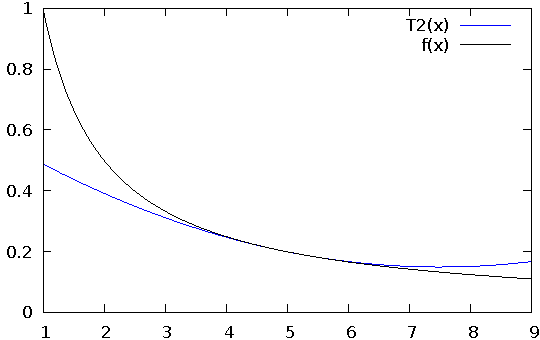
\includegraphics{figures/solns001}
\par\end{center}
\item [{\ref{exc:taylor5}:}] Mungkin pada awalnya mengejutkan, tetapi
kita tidak perlu mencari $T_{4}(x)$ untuk menjawab pertanyaan ini.
Persoalan galat sepenuhnya tercakup oleh suku sisa. Jadi, kita hanya
perlu menghitung $R_{4}(x)$. Namun, hal ini mengharuskan kita mencari
lima turunan pertama dari $f(x)$:
\begin{eqnarray*}
f(x) & = & e^{-x^{2}}\\
f'(x) & = & -2xe^{-x^{2}}\\
f''(x) & = & -2e^{-x^{2}}+(-2x)(-2xe^{-x^{2}})\\
 & = & 2(2x^{2}-1)e^{-x^{2}}\\
f'''(x) & = & 2[4xe^{-x^{2}}+(2x^{2}-1)(-2xe^{-x^{2}})]\\
 & = & -4(2x^{3}-3x)e^{-x^{2}}\\
f^{(4)}(x) & = & -4[(6x^{2}-3)e^{-x^{2}}+(2x^{3}-3x)(-2xe^{-x^{2}})]\\
 & = & -4(-4x^{4}+12x^{2}-3)e^{-x^{2}}\\
f^{(5)}(x) & = & -4[(-16x^{3}+24x)e^{-x^{2}}+(-4x^{4}+12x^{2}-3)(-2xe^{-x^{2}})]\\
 & = & -8(4x^{5}-20x^{3}+15x)e^{-x^{2}}
\end{eqnarray*}
Sekarang, $R_{4}(x)=\frac{f^{(5)}(\xi)}{5!}x^{5}=\frac{-8(4\xi^{5}-20\xi^{3}+15\xi)e^{-\xi^{2}}}{120}x^{5}=\frac{x^{5}}{15}\left(4\xi^{5}-20\xi^{3}+15\xi\right)e^{-\xi^{2}}$.
Untuk setiap nilai $x$, kita harus memaksimumkan nilai absolut dari
ekspresi ini untuk semua $\xi$ di antara 0 dan $x$. Kita dapat mengabaikan
faktor $\frac{x^{5}}{15}$ yang tidak bergantung pada $\xi$, dan
berfokus mencari ekstrem dari $\left(4\xi^{5}-20\xi^{3}+15\xi\right)e^{-\xi^{2}}$.
Kadang-kadang, pada tahap ini, ekspresi yang perlu dioptimalkan cukup
mudah untuk ditangani dengan teknik kalkulus standar---mencari titik
kritis dan mengevaluasinya. Namun, dalam kasus ini, hal itu akan melibatkan
pencarian akar-akar polinom berderajat enam. Ironisnya, teknik yang
akan kita pelajari nanti dalam mata kuliah ini akan berguna sekarang,
tetapi saat ini kita tidak memiliki cara untuk melakukannya secara
umum. Hal terbaik yang dapat kita lakukan adalah melihat grafik dan
berharap grafik tersebut membantu. Dengan menetapkan $g(\xi)=\left(4\xi^{5}-20\xi^{3}+15\xi\right)e^{-\xi^{2}}$,
kita melanjutkan dengan memplot $g(\xi)$:

\begin{center}
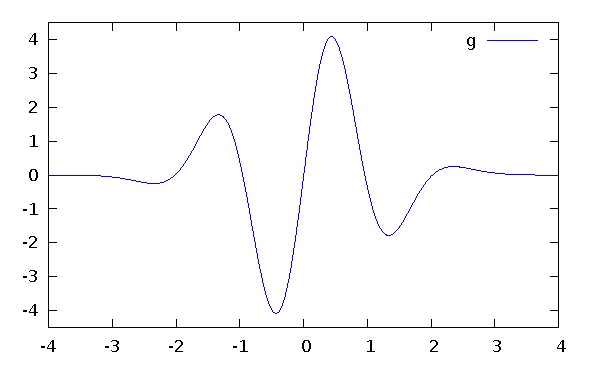
\includegraphics{figures/solns002}.
\par\end{center}

Dengan mengingat tujuan untuk memaksimumkan, masuk akal untuk memperhatikan
ekstrem-ekstrem relatif. Fungsi tersebut tampaknya memiliki 6 ekstrem
relatif dan mendekati nol ketika $\xi$ mendekati $\pm\infty$. Untuk
memastikan bahwa pengamatan ini benar, kita mulai dengan menghitung
$g'(\xi)=-(8\xi^{6}-60\xi^{4}+90\xi^{2}-15)%e^{-\xi^{2}}\ensuremath{}
$. Karena polinom derajat enam memiliki paling banyak 6 akar berbeda,
$g$ memiliki paling banyak 6 ekstrem relatif. Karena kita melihat
6 ekstrem relatif pada grafik, tidak ada yang lain. Selain itu, 
\[
\lim_{\xi\to\pm\infty}-(8\xi^{6}-60\xi^{4}+90\xi^{2}-15)%e^{-\xi^{2}}=0
\]
karena faktor eksponensial mendominasi faktor polinom. Kita mungkin
tidak terpikir untuk mempertimbangkan kedua fakta ini jika bukan karena
grafik tersebut. Namun, masih ada lagi. Grafik tersebut tampaknya
merupakan fungsi ganjil. Sekali lagi, kita dapat memverifikasi bahwa
memang demikian: 
\begin{eqnarray*}
g(-\xi) & = & \left(4(-\xi)^{5}-20(-\xi)^{3}+15(-\xi)\right)e^{-(-\xi)^{2}}\\
 & = & -(4\xi^{5}-20\xi^{3}+15\xi)e^{-\xi^{2}}\\
 & = & -g(\xi).
\end{eqnarray*}
Karena simetri ini, kita dapat berfokus mencari ekstrem untuk nilai
positif dari $\xi$. Dan karena pada akhirnya kita ingin memaksimumkan
$|g|$, sekarang tepat untuk mempertimbangkan grafik $|g(\xi)|$ pada
$\xi\in[0,4]$:

\begin{center}
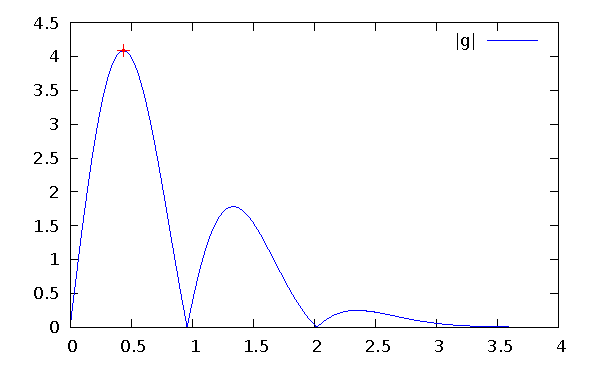
\includegraphics{figures/solns003}.
\par\end{center}

Akhirnya, kita dapat menangani pemaksimuman tersebut. Maksimum relatif
yang ditandai dengan tanda tambah merah akan menjadi kunci jawaban.
Misalkan koordinat titik ini adalah $(\hat{\xi},g(\hat{\xi}))$. Kemudian,
karena $|g(\xi)|$ meningkat pada interval dari 0 hingga $\hat{\xi}$,
kita dapat menyimpulkan bahwa
\[
\max_{\xi\in[0,x]}|g(\xi)|=|g(x)|=g(x)
\]
untuk semua $x$ di antara 0 dan $\hat{\xi}$. Selain itu, 
\[
\max_{\xi\in[0,x]}|g(\xi)|=|g(\hat{\xi})|=g(\hat{\xi})
\]
untuk semua $x\geq\hat{\xi}$. Berdasarkan simetri, kita dapat menyimpulkan
bahwa ${\displaystyle \max_{\xi\in[x,0]}|g(\xi)|}=g(x)$ untuk $x$
di antara $-\hat{\xi}$ dan 0, serta ${\displaystyle \max_{\xi\in[x,0]}|g(\xi)|}=g(\hat{\xi})$
berlaku untuk semua $x\leq-\hat{\xi}$ yang besar. Dengan menggabungkan
semuanya,
\[
|T_{4}(x)-f(x)|=|R_{4}(x)|\leq\begin{cases}
\frac{x^{5}}{15}g(x) & \mbox{ jika }|x|<\hat{\xi}\\
\frac{x^{5}}{15}g(\hat{\xi}) & \mbox{ jika }|x|\geq\hat{\xi}
\end{cases}.
\]
Harus diakui, kita tidak mengetahui nilai $\hat{\xi}$ atau $g(\hat{\xi})$,
tetapi kita dapat menghampirinya menggunakan kalkulator grafik: $(\hat{\xi},g(\hat{\xi}))\approx(.43607,4.0892)$
yang besar.
\end{description}

\section*{Bagian \ref{sec:Speed}}
\begin{description}
\item [{\ref{exc:convergence}:}] Kita perlu mencari $\alpha$ sedemikian
sehingga $\lim_{n\to\infty}\frac{1/3^{e^{n+1}}}{\left(1/3^{e^{n}}\right)^{\alpha}}=\lambda$
untuk suatu $\lambda\neq0$. Jadi, mengamati $\frac{1/3^{e^{n+1}}}{\left(1/3^{e^{n}}\right)^{\alpha}}$
dengan saksama seharusnya membantu:
\begin{eqnarray*}
\frac{1/3^{e^{n+1}}}{\left(1/3^{e^{n}}\right)^{\alpha}} & = & \frac{\left(3^{e^{n}}\right){}^{\alpha}}{3^{e^{n+1}}}\\
 & = & \frac{3^{\alpha e^{n}}}{3^{e^{n+1}}}\\
 & = & \frac{3^{\alpha e^{n}}}{3^{e\cdot e^{n}}}.
\end{eqnarray*}
Akibatnya, jika $\alpha=e$, maka $\frac{1/3^{e^{n+1}}}{\left(1/3^{e^{n}}\right)^{\alpha}}=1$,
sehingga diperoleh bahwa $\lim_{n\to\infty}\frac{1/3^{e^{n+1}}}{\left(1/3^{e^{n}}\right)^{\alpha}}=1$.
Oleh karena itu, orde kekonvergenannya adalah $\alpha=e$.
\item [{\ref{exc:convergence-1}:}] Kita perlu mencari $\alpha$ sedemikian
sehingga $\lim_{n\to\infty}\frac{\left|\frac{2^{2^{n+1}}-2}{2^{2^{n+1}}+3}-1\right|}{\left|\frac{2^{2^{n}}-2}{2^{2^{n}}+3}-1\right|^{\alpha}}=\lambda$
untuk suatu $\lambda\neq0$. Jadi, mengamati $\frac{\left|\frac{2^{2^{n+1}}-2}{2^{2^{n+1}}+3}-1\right|}{\left|\frac{2^{2^{n}}-2}{2^{2^{n}}+3}-1\right|^{\alpha}}$
dengan saksama seharusnya membantu:
\begin{eqnarray*}
\frac{\left|\frac{2^{2^{n+1}}-2}{2^{2^{n+1}}+3}-1\right|}{\left|\frac{2^{2^{n}}-2}{2^{2^{n}}+3}-1\right|^{\alpha}} & = & \frac{\left|\frac{2^{2^{n+1}}-2}{2^{2^{n+1}}+3}-\frac{2^{2^{n+1}}+3}{2^{2^{n+1}}+3}\right|}{\left|\frac{2^{2^{n}}-2}{2^{2^{n}}+3}-\frac{2^{2^{n}}+3}{2^{2^{n}}+3}\right|^{\alpha}}\\
 & = & \frac{\left|\frac{-5}{2^{2^{n+1}}+3}\right|}{\left|\frac{-5}{2^{2^{n}}+3}\right|^{\alpha}}\\
 & = & 5^{1-\alpha}\frac{\left(2^{2^{n}}+3\right)^{\alpha}}{2^{2^{n+1}}+3}.
\end{eqnarray*}
Jika $\alpha=2$, suku-suku utama pada pembilang dan penyebut pecahan
yang dihasilkan akan sama. Ini merupakan bukti kuat bahwa $\alpha=2$
adalah pilihan yang tepat. Mari kita coba:
\begin{eqnarray*}
5^{1-2}\frac{\left(2^{2^{n}}+3\right)^{2}}{2^{2^{n+1}}+3} & = & \frac{1}{5}\cdot\frac{2^{2\cdot2^{n}}+6\cdot2^{2^{n}}+3}{2^{2^{n+1}}+3}\\
 & = & \frac{1}{5}\cdot\frac{2^{2^{n+1}}+6\cdot2^{2^{n}}+3}{2^{2^{n+1}}+3}\\
 & = & \frac{1}{5}\cdot\frac{1+6\cdot2^{-2^{n}}+3\cdot2^{-2^{n+1}}}{1+3\cdot2^{-2^{n+1}}}.
\end{eqnarray*}
Pada langkah terakhir, kita telah membagi pembilang dan penyebut dengan
$2^{2^{n+1}}$ agar pengambilan limit saat $n$ mendekati $\infty$
menjadi mudah:
\begin{eqnarray*}
\lim_{n\to\infty}\frac{\left|\frac{2^{2^{n+1}}-2}{2^{2^{n+1}}+3}-1\right|}{\left|\frac{2^{2^{n}}-2}{2^{2^{n}}+3}-1\right|^{2}} & = & \lim_{n\to\infty}\frac{1}{5}\cdot\frac{1+6\cdot2^{-2^{n}}+3\cdot2^{-2^{n+1}}}{1+3\cdot2^{-2^{n+1}}}\\
 & = & \frac{1}{5}.
\end{eqnarray*}
Jadi, orde kekonvergenannya adalah $\alpha=2$.
\item [{\ref{exc:convergence-3}:}] Pertama, kita mencari fungsi berbentuk
$\frac{C}{n^{p}}$ atau berbentuk $\frac{K}{a^{n}}$ yang sekurang-kurangnya
sebesar $\left|\frac{\sin n}{\sqrt{n}}\right|$ untuk $n$ yang besar.
Namun, pada akhirnya kita menginginkan fungsi terkecil yang memenuhi
hal tersebut (hingga suatu konstanta). Kunci penyelesaiannya adalah
memperhatikan bahwa $|\sin n|\leq1$ untuk semua $n$:
\[
\left|\frac{\sin n}{\sqrt{n}}\right|=\frac{|\sin n|}{\sqrt{n}}\leq\frac{1}{\sqrt{n}}=\frac{1}{n^{1/2}}.
\]
Karena pertidaksamaan ini tidak berlaku untuk pangkat yang lebih tinggi
dari $n$, laju kekonvergenannya adalah $O\left(\frac{1}{n^{1/2}}\right)$.
\item [{\ref{exc:convergence-4}:}] Pertama, kita mencari fungsi berbentuk
$\frac{C}{n^{p}}$ atau berbentuk $\frac{K}{a^{n}}$ yang sekurang-kurangnya
sebesar $\left|\frac{4}{10^{n}+35n+9}\right|$ untuk $n$ yang besar.
Namun, pada akhirnya kita menginginkan fungsi terkecil yang memenuhi
hal tersebut (hingga suatu konstanta). Kunci penyelesaiannya adalah
memperhatikan bahwa $10^{n}+35n+9>10^{n}$ untuk semua $n$:
\[
\left|\frac{4}{10^{n}+35n+9}\right|=\frac{4}{10^{n}+35n+9}\leq\frac{4}{10^{n}}.
\]
Karena pertidaksamaan ini tidak berlaku untuk basis mana pun yang
lebih besar dari 10, laju kekonvergenannya adalah $O\left(\frac{1}{10^{n}}\right)$.
\item [{\ref{exc:convergence-5}:}] Pertama, kita mencari fungsi berbentuk
$\frac{C}{n^{p}}$ atau berbentuk $\frac{K}{a^{n}}$ yang sekurang-kurangnya
sebesar $\left|\frac{4}{10^{n}-35n-9}\right|$ untuk $n$ yang besar.
Namun, pada akhirnya kita menginginkan fungsi terkecil yang memenuhi
hal tersebut (hingga suatu konstanta). Kunci penyelesaiannya adalah
menangani fakta bahwa $10^{n}-35n-9<10^{n}$ untuk semua $n$:
\begin{eqnarray*}
\left|\frac{4}{10^{n}-35n-9}\right| & = & \frac{8}{2\cdot10^{n}-70n-18}\\
 & = & \frac{8}{10^{n}+(10^{n}-70n-18)}\\
 & \leq & \frac{8}{10^{n}}
\end{eqnarray*}
untuk $n$ yang cukup besar karena $10^{n}-70n-18\geq0$ untuk semua
$n$ yang besar. Karena tidak ada pertidaksamaan serupa yang berlaku
untuk basis mana pun yang lebih besar dari 10, laju kekonvergenannya
adalah $O\left(\frac{1}{10^{n}}\right)$. Perhatikan bahwa laju kekonvergenan
kita sama seperti dalam soal \ref{exc:convergence-4} meskipun kita
memperoleh konstanta yang lebih besar. Laju kekonvergenan tidak bergantung
pada konstanta yang diperlukan dalam pertidaksamaan tersebut.
\item [{\ref{exc:convergence-8}:}] Pertama, kita mencari fungsi berbentuk
$\frac{C}{n^{p}}$ atau berbentuk $\frac{K}{a^{n}}$ yang sekurang-kurangnya
sebesar $\left|\frac{n^{2}}{2^{n}}\right|$ untuk $n$ yang besar.
Namun, pada akhirnya kita menginginkan fungsi terkecil yang memenuhi
hal tersebut (hingga suatu konstanta). Misalkan $2>\varepsilon>0$
sebarang. Perhatikan bahwa $\frac{n^{2}}{2^{n}}\leq\frac{1}{(2-\varepsilon)^{n}}$
untuk $n$ yang besar dengan menyusun ulang pertidaksamaan sebagai
berikut: $\frac{n^{2}}{2^{n}}\leq\frac{1}{(2-\varepsilon)^{n}}$ jika
dan hanya jika $n^{2}\leq\frac{2^{n}}{(2-\varepsilon)^{n}}$ jika
dan hanya jika $n^{2}\leq\left(\frac{2}{2-\varepsilon}\right)^{n}$.
Kita tahu pertidaksamaan terakhir ini benar untuk $n$ yang cukup
besar karena $\frac{2}{2-\varepsilon}>1$, dan fungsi eksponensial
mendominasi fungsi polinom. Oleh karena itu, kita dapat menggunakan
laju kekonvergenan berbentuk $O\left(\frac{1}{(2-\varepsilon)^{n}}\right)$,
tetapi tidak ada fungsi terkecil semacam itu. Oleh karena itu, kita
cukup menggunakan $O\left(\frac{n^{2}}{2^{n}}\right)$ sebagai laju
kekonvergenan.
\item [{\ref{exc:convergence-10}:}] Salah satu berkas \texttt{.m} yang
mungkin adalah: \begin{verbatim}
for j=0:9
  disp(7^j)
end%for 
\end{verbatim}
\item [{\ref{exc:convergence-11}:}] Salah satu berkas \texttt{.m} yang
mungkin adalah: \begin{verbatim}
f=@(x) (2^(2^x)-2)/(2^(2^x)+3);
n=[0,1,2,4,6,10];
for i=1:6
  disp(f(n(i)))
end%for
\end{verbatim}
\item [{\ref{exc:convergence-12}:}] Untuk barisan dengan orde kekonvergenan
linear, kita tahu jumlah angka signifikan bertambah sekitar $-\log\lambda$
pada setiap iterasi, sehingga kita perlu mencari $k$ terkecil sedemikian
sehingga $1-k\log(0.5)\geq12$. Menyelesaikan persamaan $1-k\log(0.5)=12$
untuk $k$:
\begin{eqnarray*}
1-k\log(0.5) & = & 12\\
-k\log(0.5) & = & 11\\
k & = & \frac{11}{-\log(0.5)}\approx36.54.
\end{eqnarray*}
Oleh karena itu, menurut aturan praktis, diperlukan 37 iterasi. Ingat,
taksiran ini hanya baik selama $\frac{|p_{n+1}-p|}{|p_{n}-p|}\approx\lambda$.
Jadi, jika nilai sebenarnya dari rasio tersebut jauh berbeda dari
$\lambda$, taksiran 37 iterasi dapat meleset jauh.
\end{description}

\section*{Bagian \ref{sec:Recursion}}
\begin{description}
\item [{\ref{exc:recursion-1}:}] (a) \texttt{trominos.m} dapat diunduh
di \href{http://lqbrin.github.io/tea-time-numerical/ancillaries.html}{situs pendamping}.\begin{verbatim}
%%%%%%%%%%%%%%%%%%%%%%%%%%%%%%%%%%%%%%%%%%%%%%%%%%%%%%%%%
%  trominos() written by Leon Q. Brin 14 February 2013  %
%       is a recursively defined function for           %
%       calculating the number of trominos needed to    %
%       cover an n X n grid of squares, save one corner %
%  INPUT: nonnegative integer n.                        %
%  OUTPUT: T(n)                                         %
%%%%%%%%%%%%%%%%%%%%%%%%%%%%%%%%%%%%%%%%%%%%%%%%%%%%%%%%%
function ans = trominos(n)
  if (n==0)
    ans = 0;
  else
    ans = 1+4*trominos(n-1);
  end%if
end%function
\end{verbatim}(b) \begin{verbatim}
octave:1> trominos(10)
ans =  349525 
\end{verbatim}
\item [{\ref{exc:recursion-2}:}] (a) 7. Ikuti urutan gerakan berikut:

\begin{center}
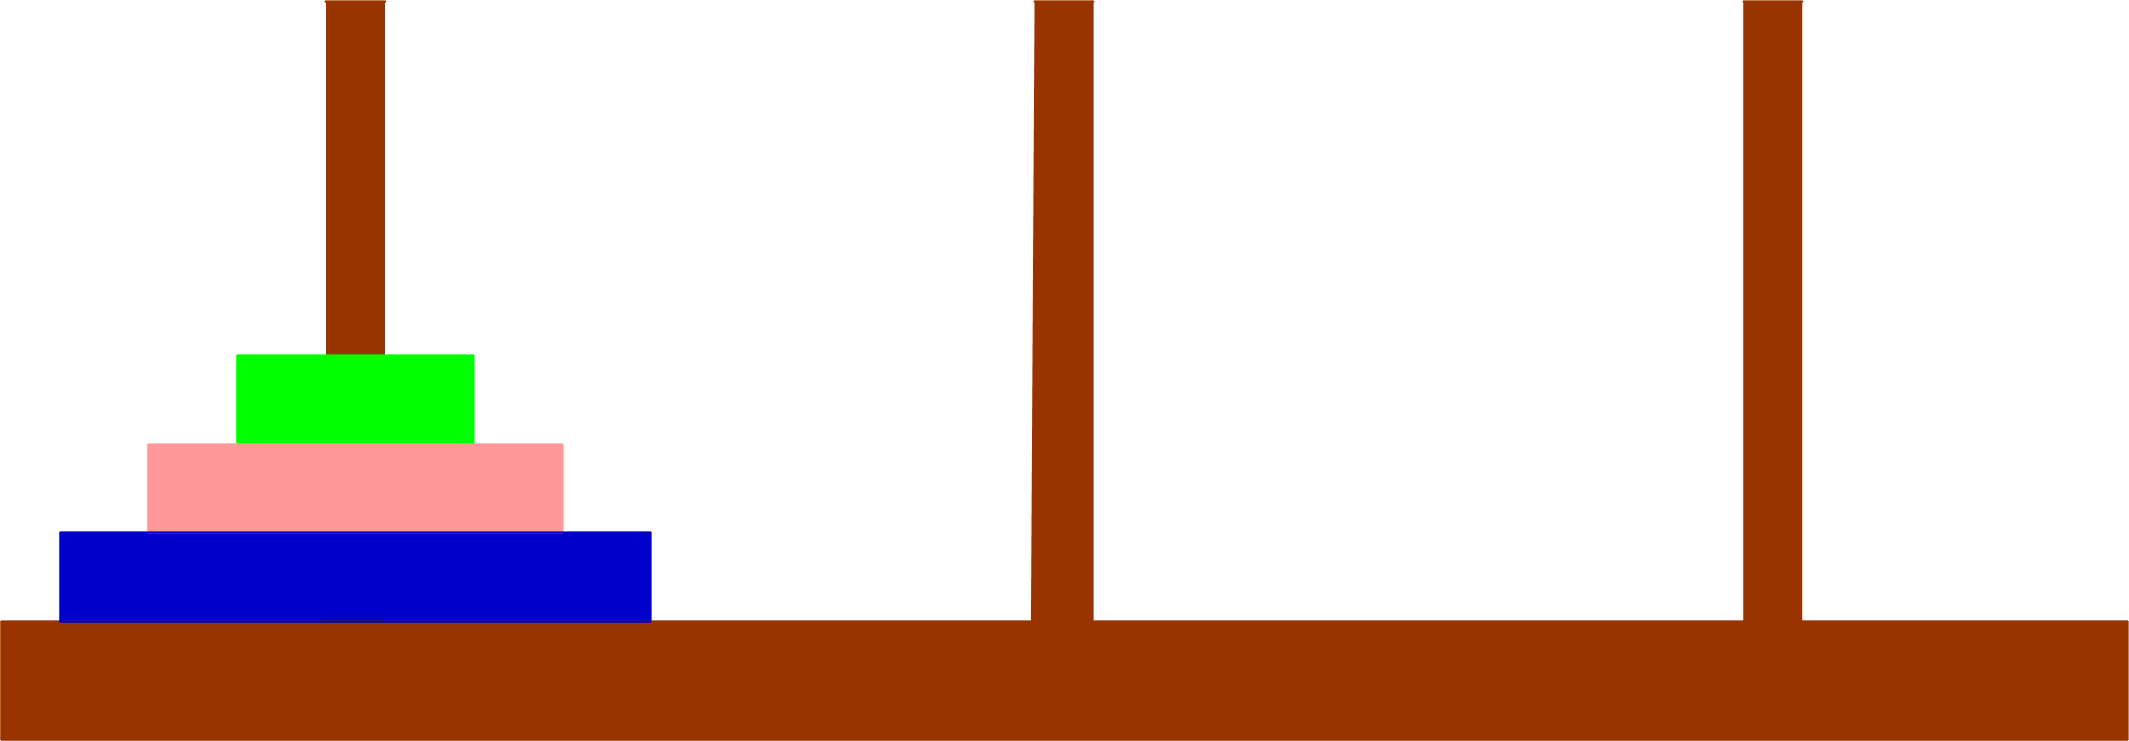
\includegraphics[scale=0.2]{figures/hanoi3disk-0} \hfill{} 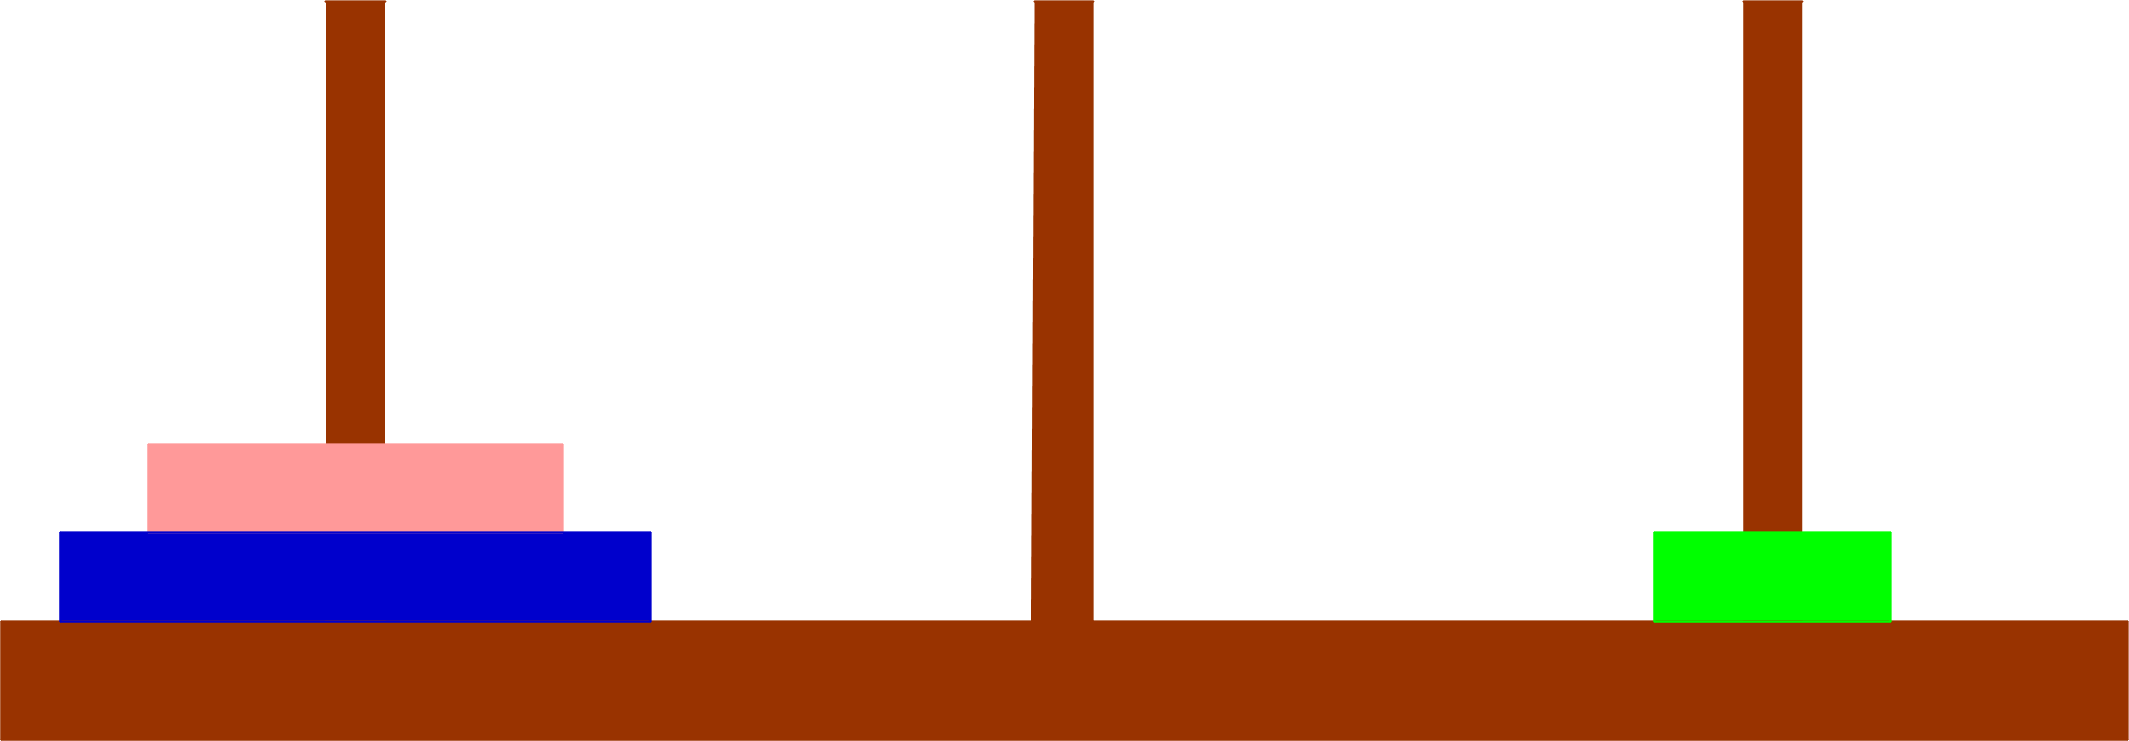
\includegraphics[scale=0.2]{figures/hanoi3disk-1}
\hfill{} 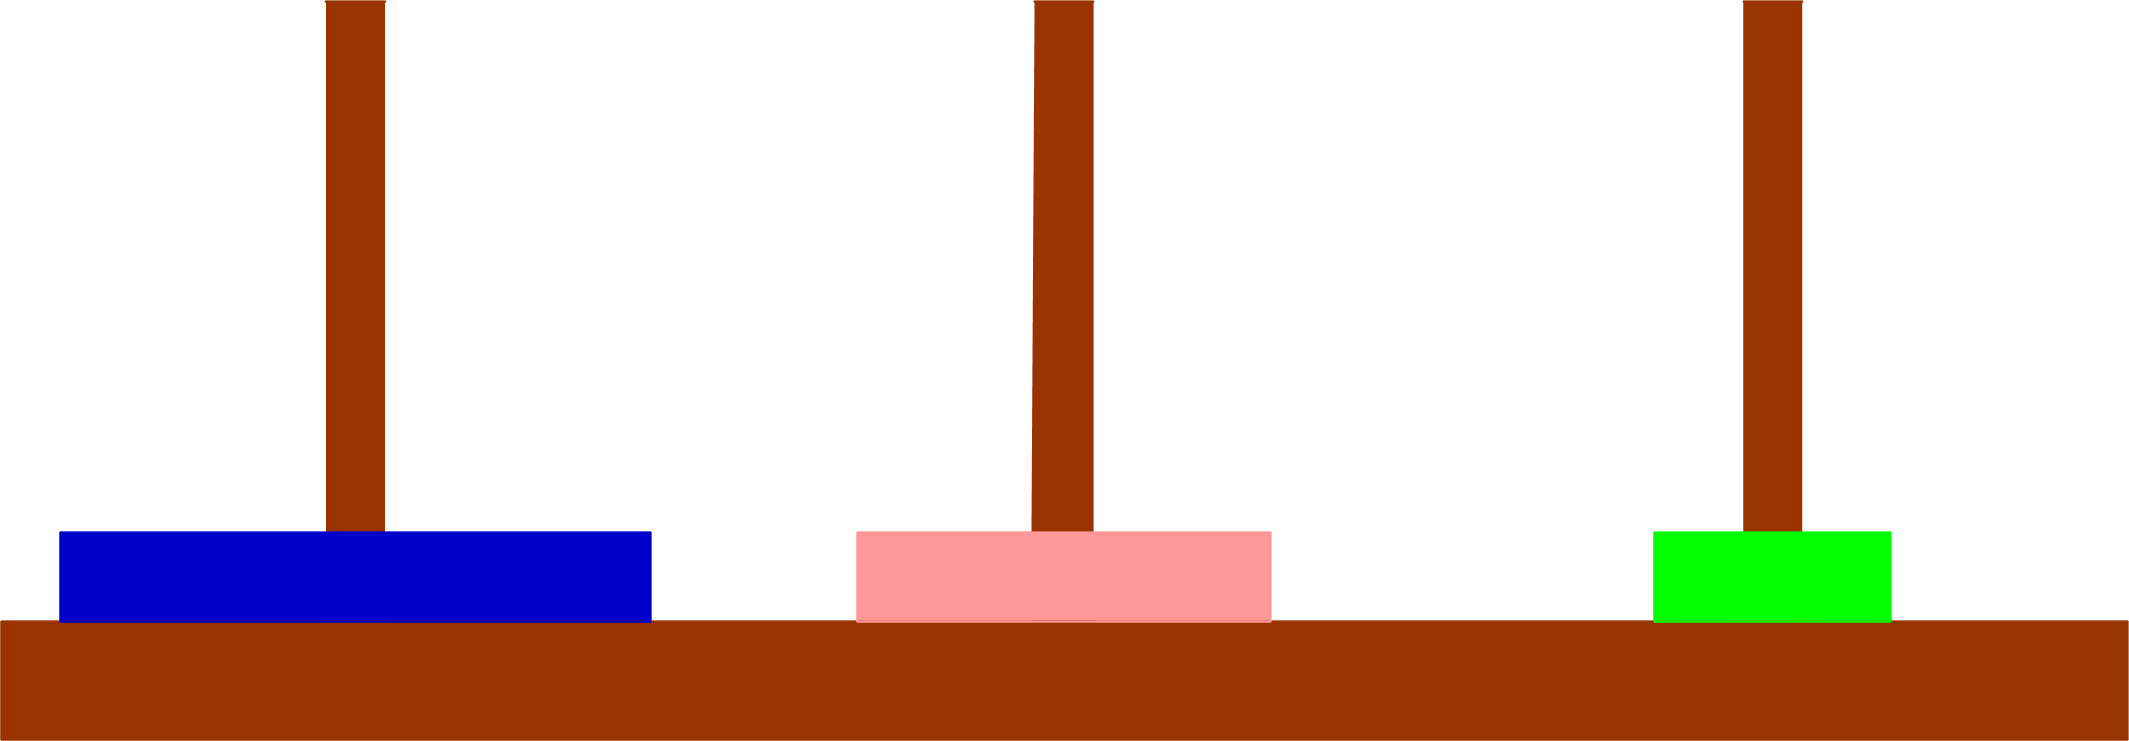
\includegraphics[scale=0.2]{figures/hanoi3disk-2}
\par\end{center}

\begin{center}
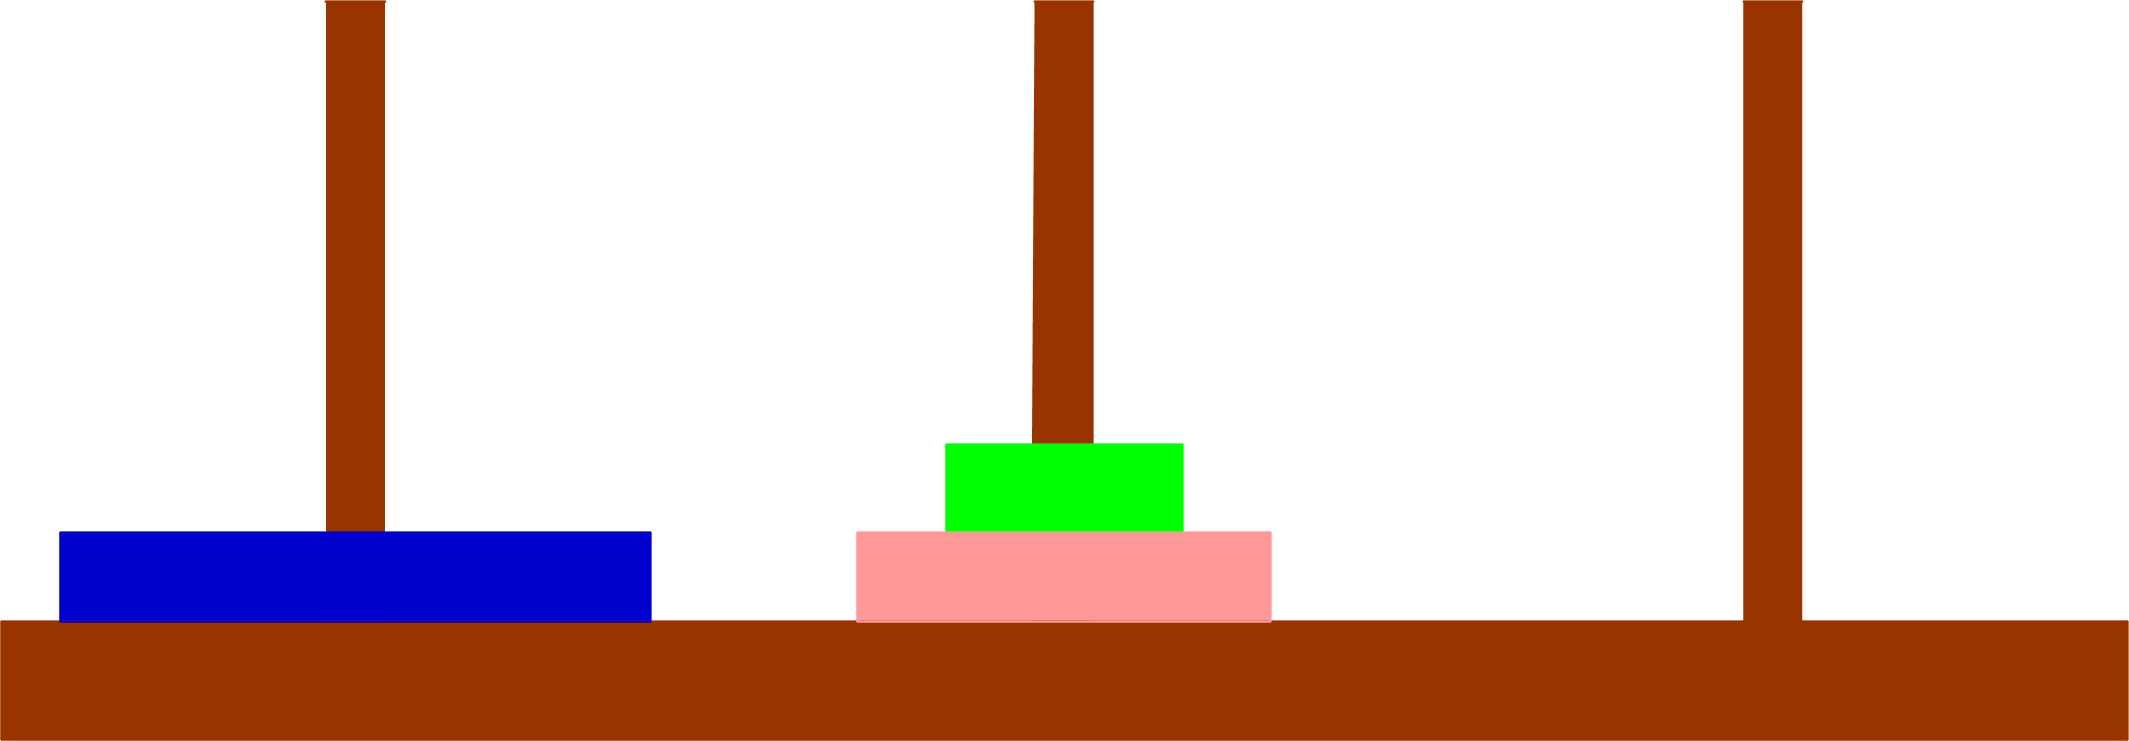
\includegraphics[scale=0.2]{figures/hanoi3disk-3} \hfill{} 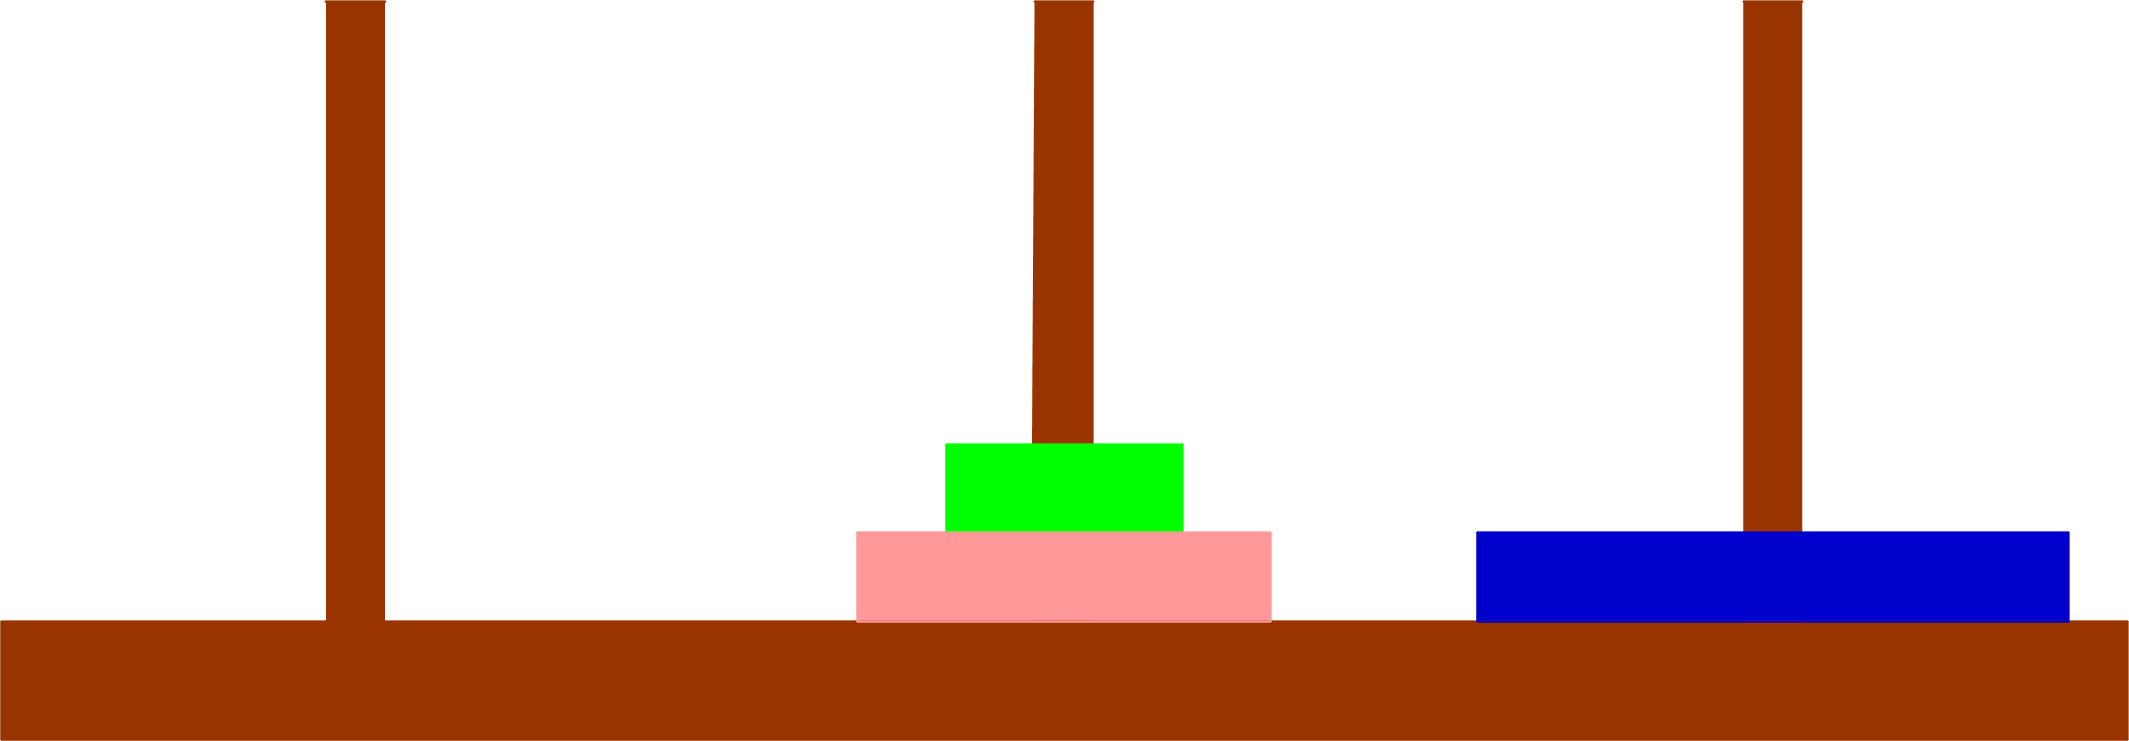
\includegraphics[scale=0.2]{figures/hanoi3disk-4}
\hfill{} 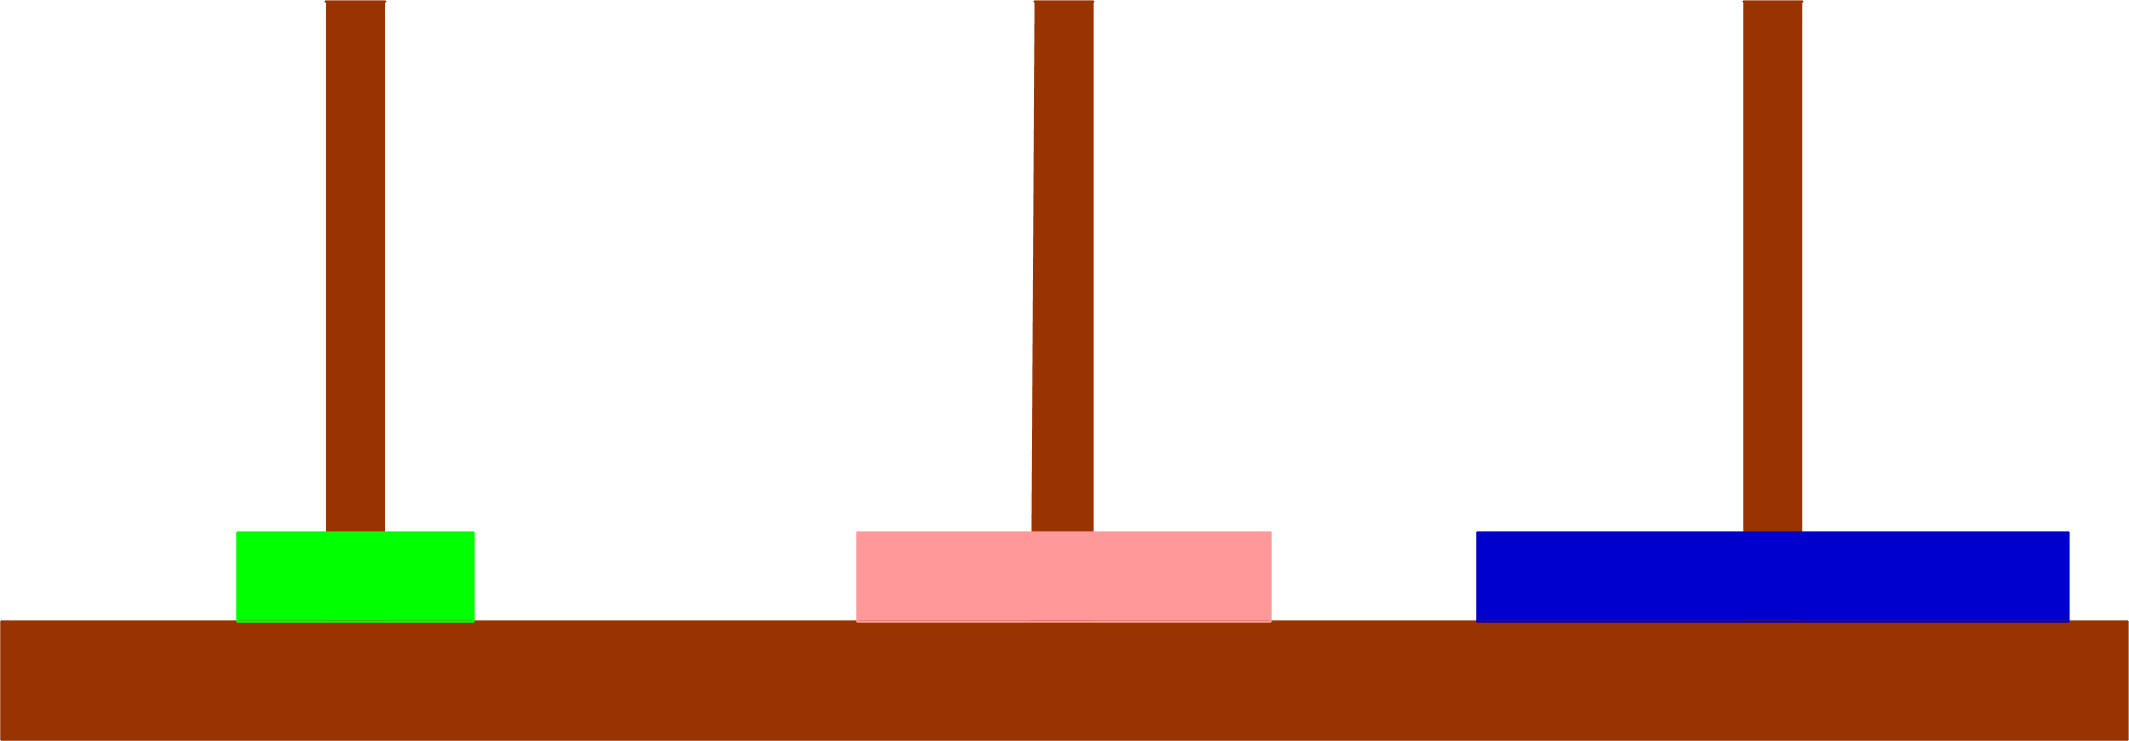
\includegraphics[scale=0.2]{figures/hanoi3disk-5}
\par\end{center}

\hfill{} 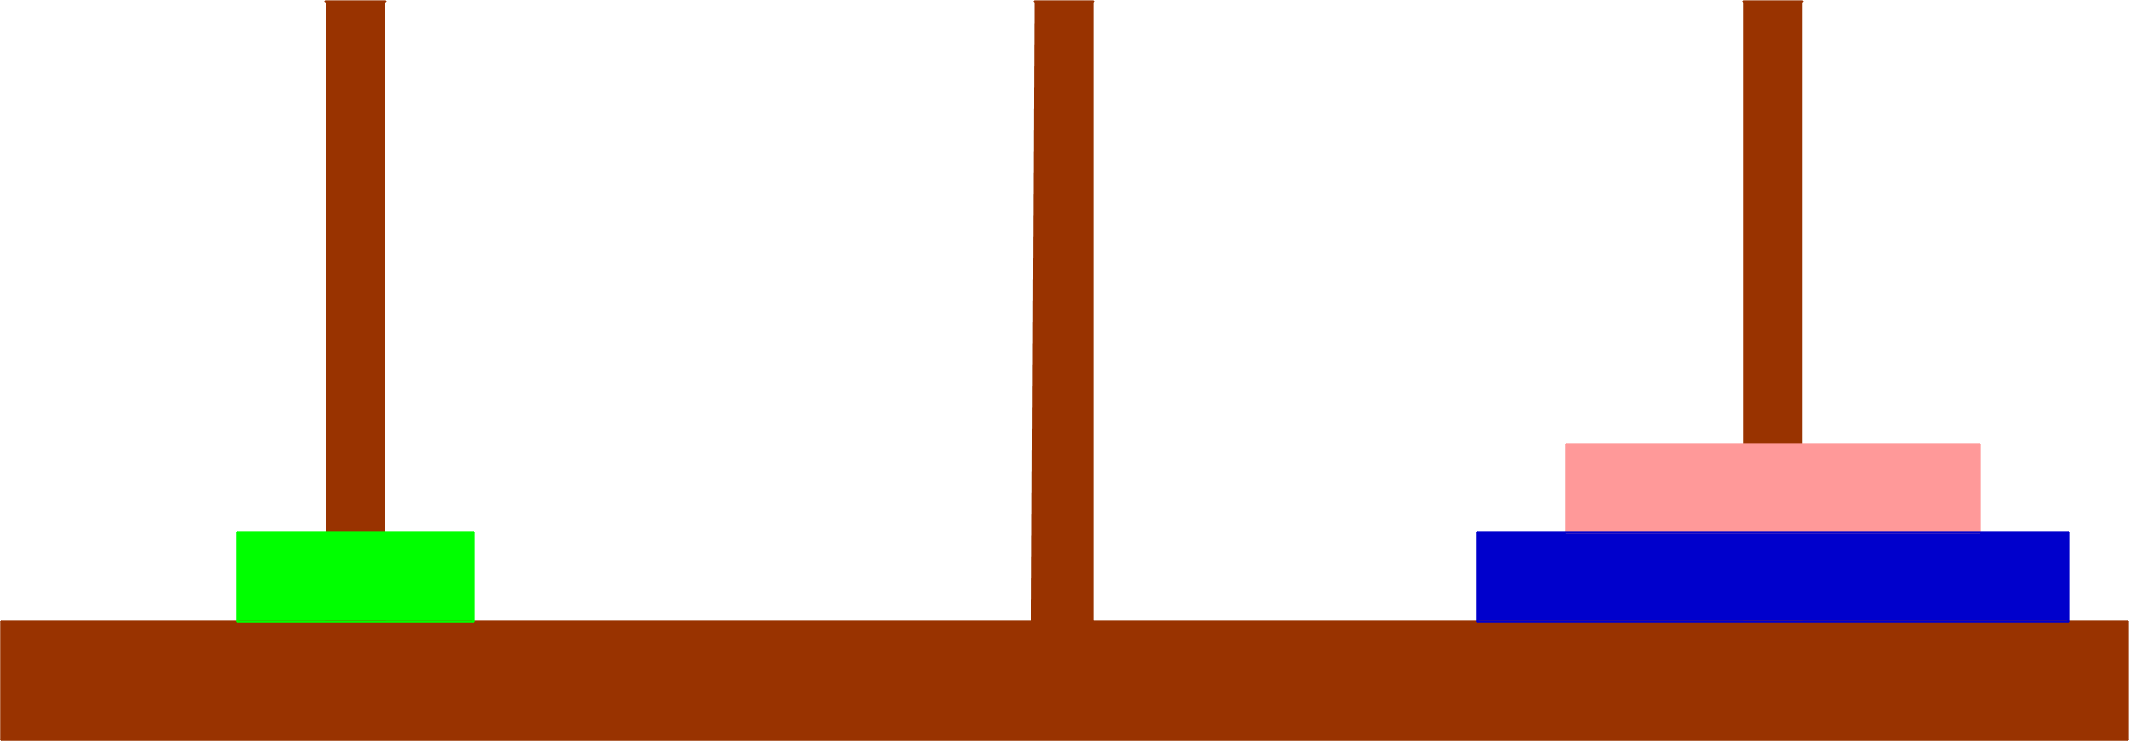
\includegraphics[scale=0.2]{figures/hanoi3disk-6} \hfill{}
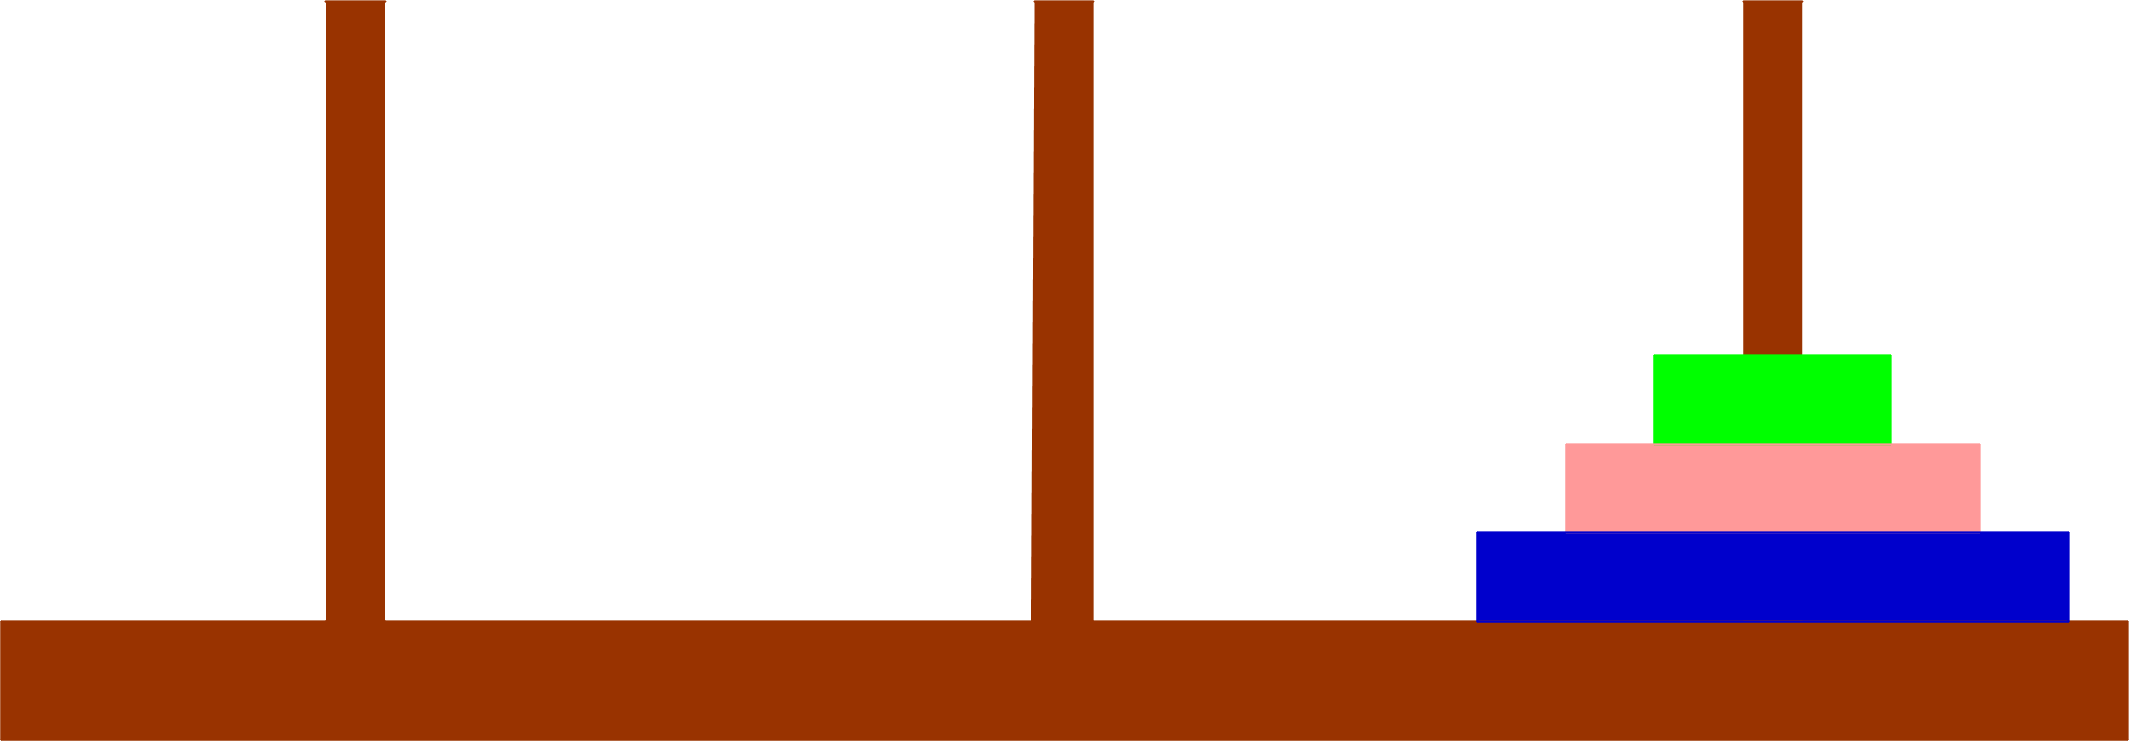
\includegraphics[scale=0.2]{figures/hanoi3disk-7} \hfill{}\\
(b) i. Perhatikan rangkaian gerakan berikut.

\begin{center}
\hfill{} 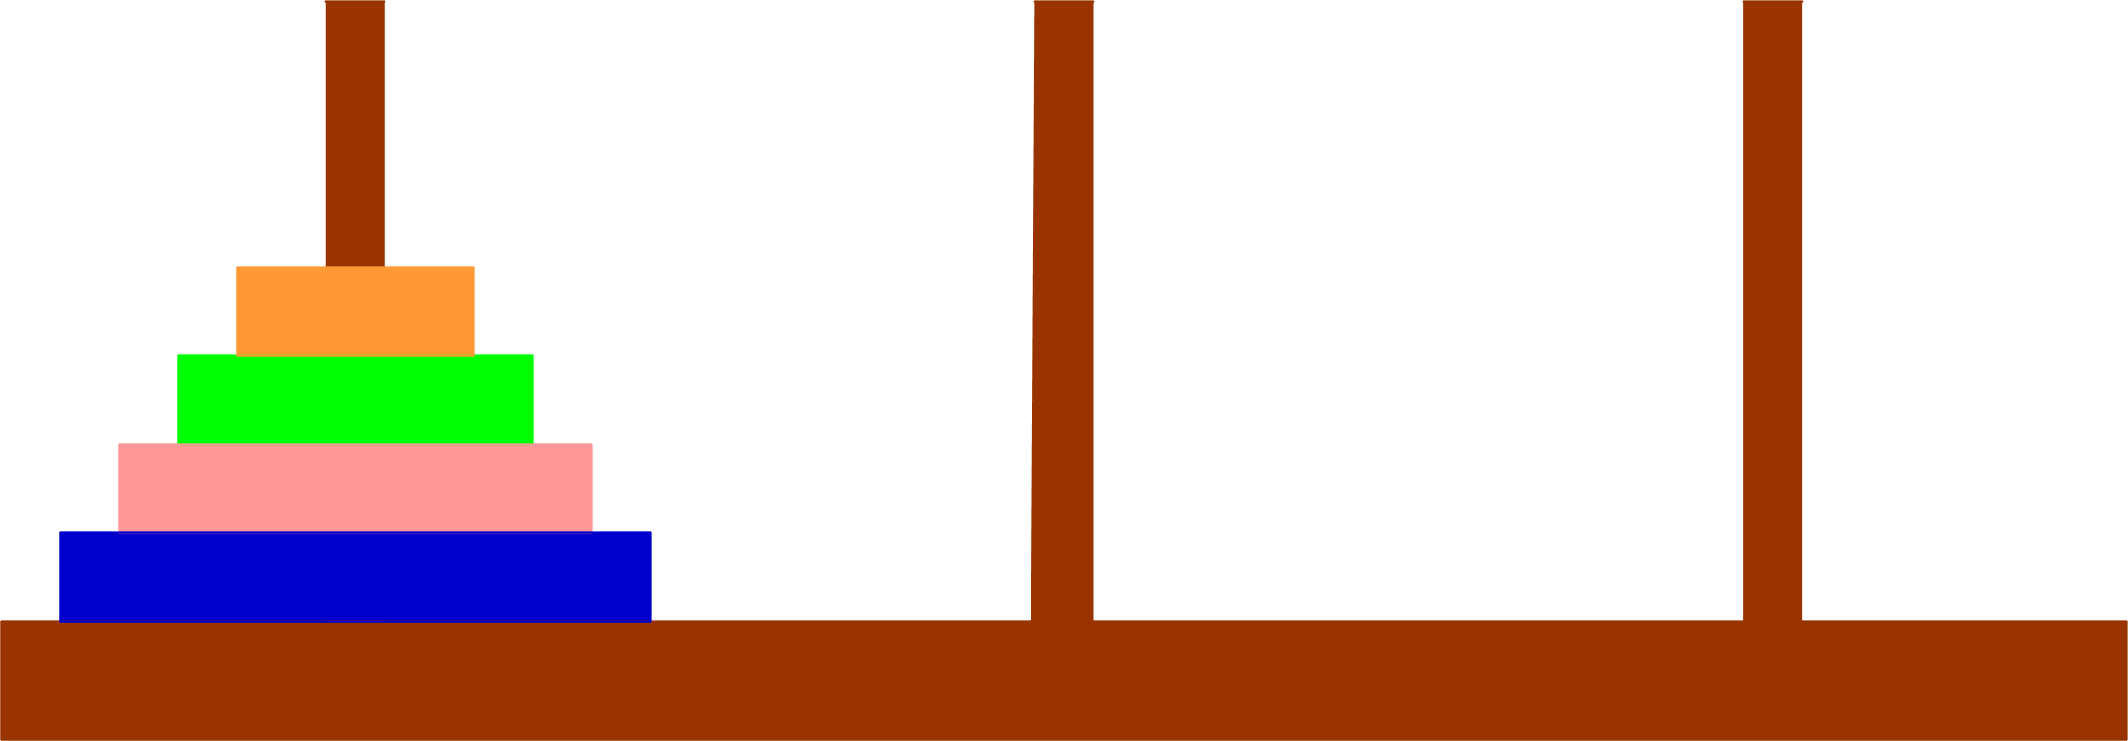
\includegraphics[scale=0.2]{figures/hanoi4disk-0} \hfill{}
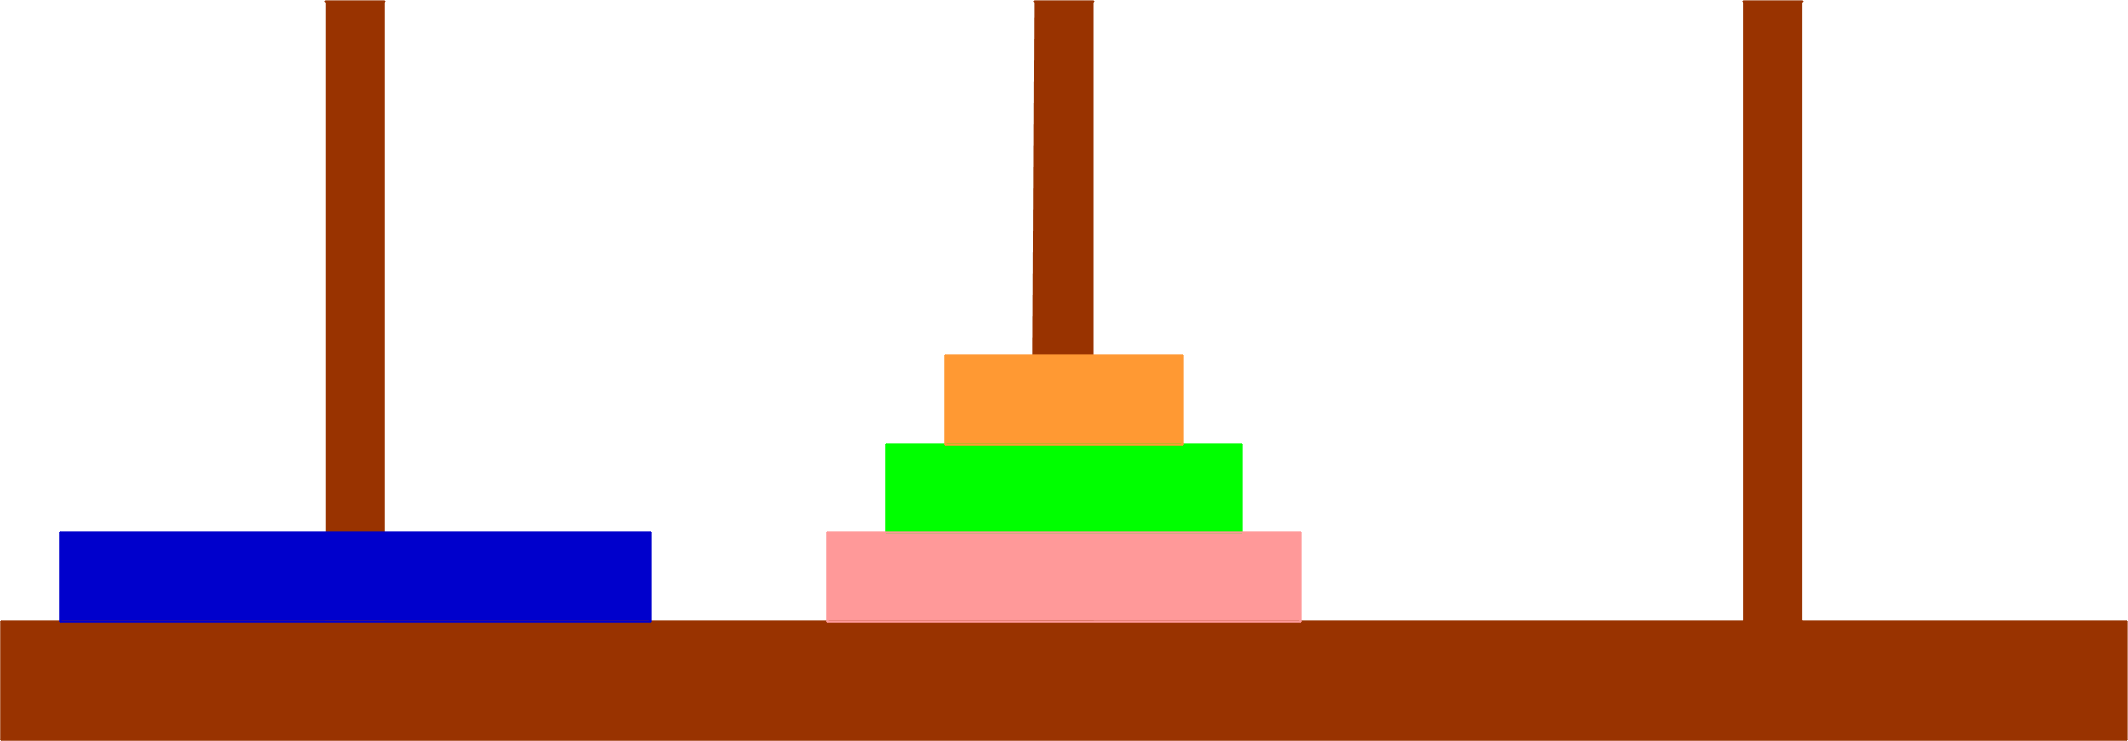
\includegraphics[scale=0.2]{figures/hanoi4disk-1} \hfill{}
\par\end{center}

\begin{center}
\hfill{} 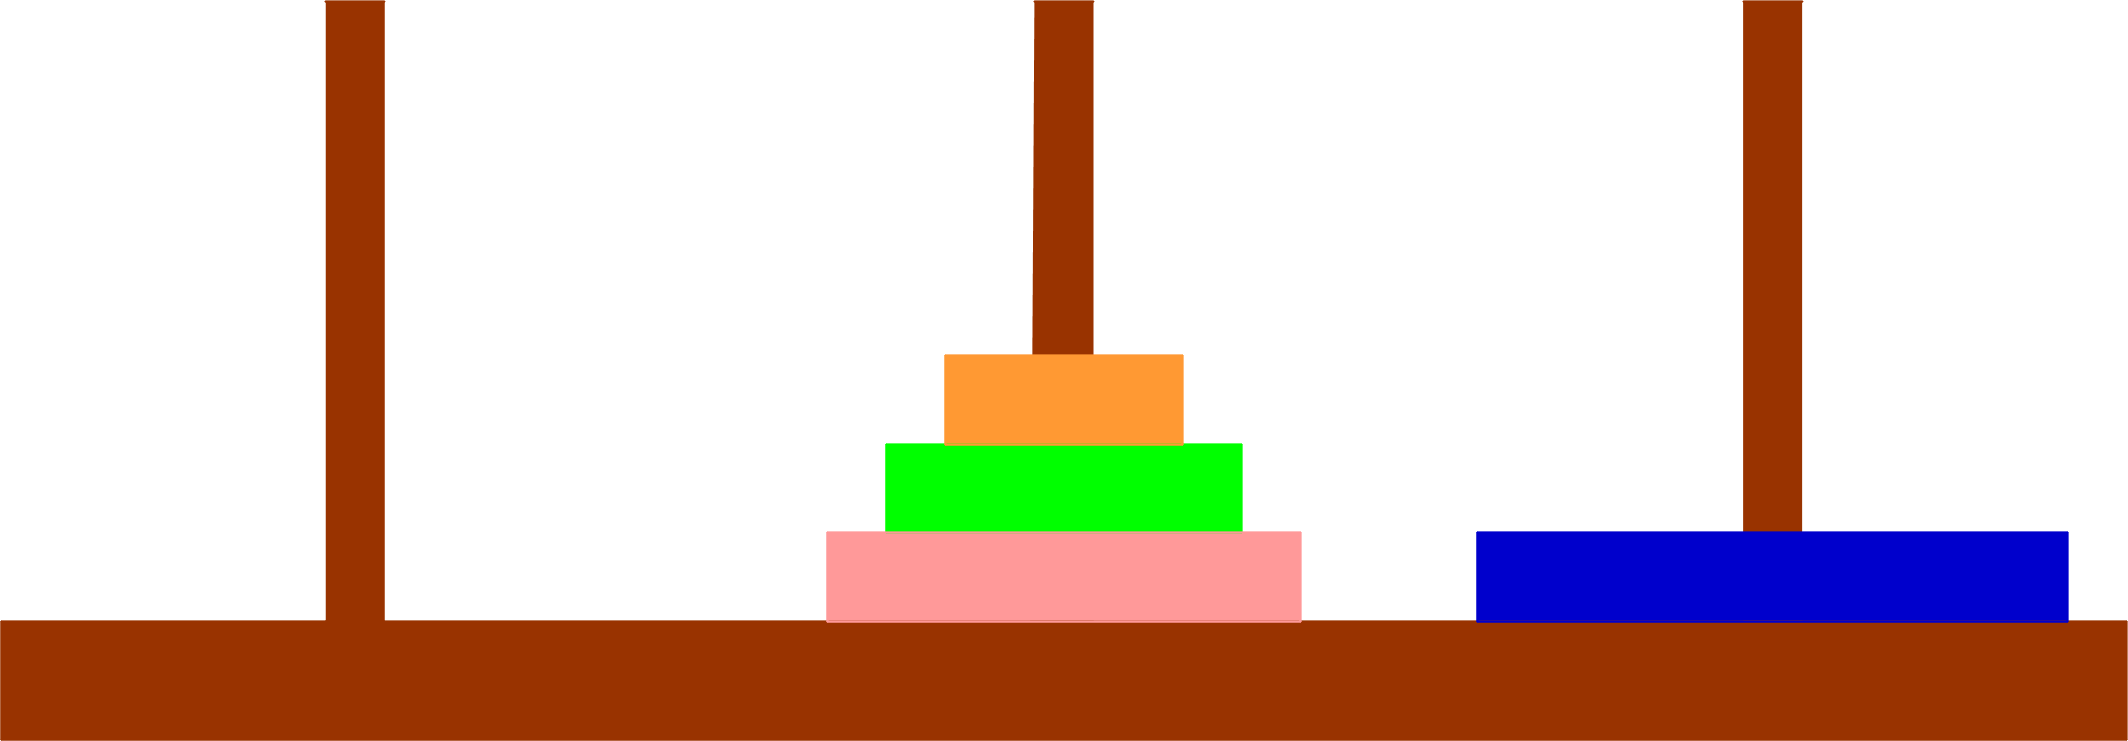
\includegraphics[scale=0.2]{figures/hanoi4disk-2} \hfill{}
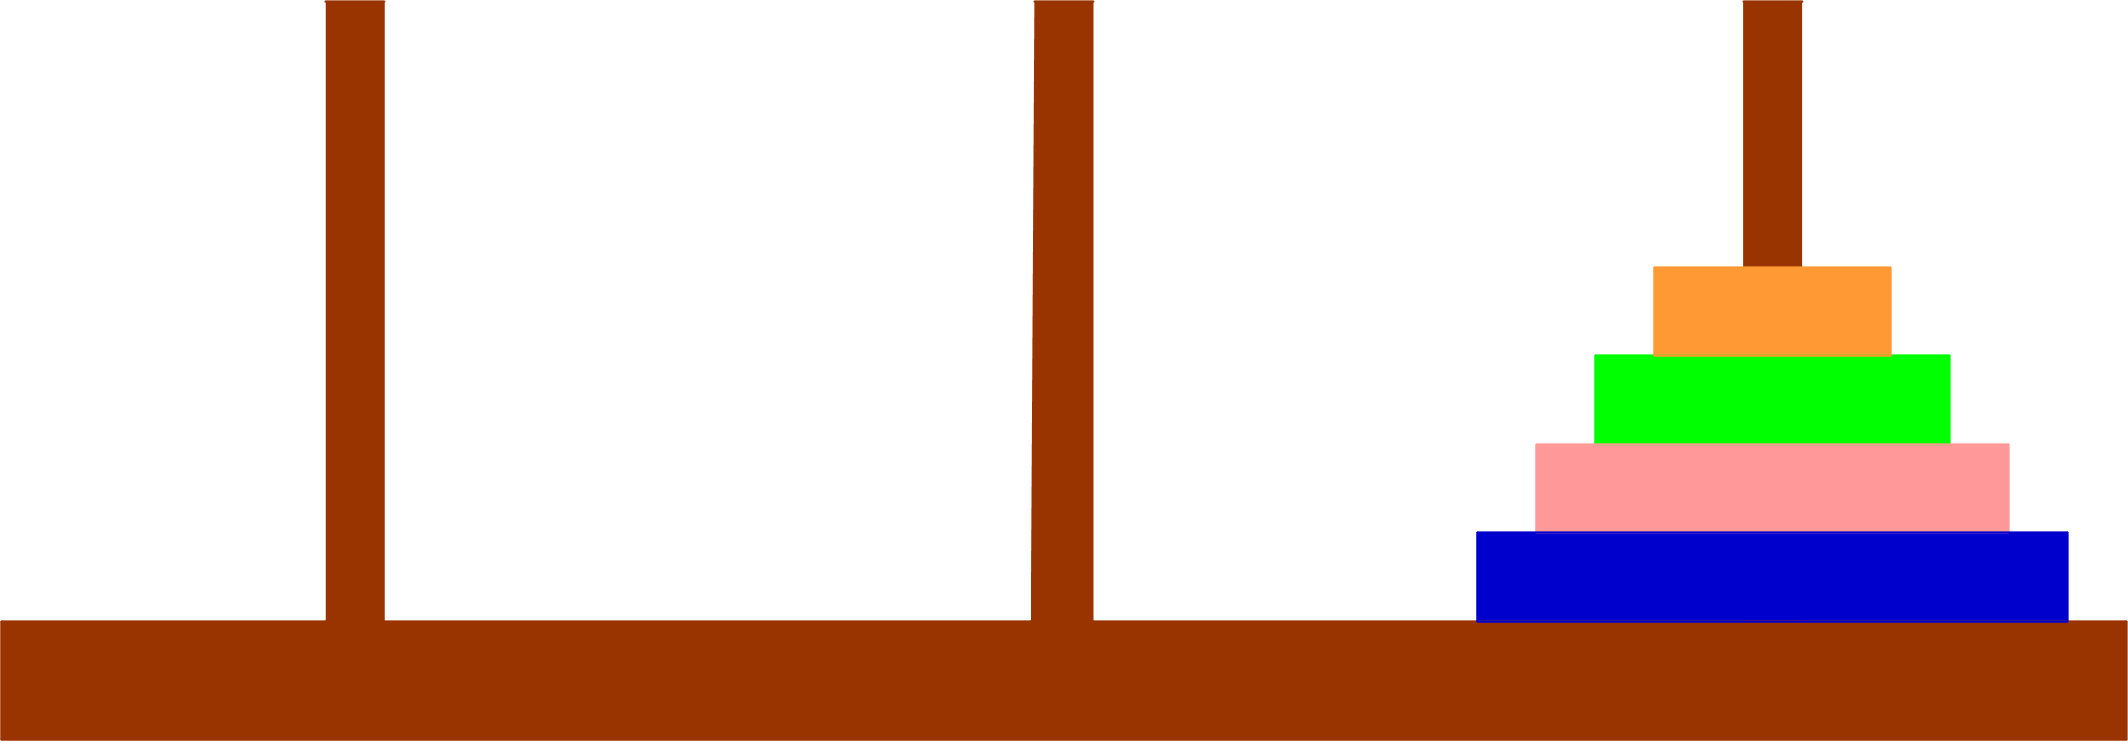
\includegraphics[scale=0.2]{figures/hanoi4disk-3} \hfill{} 
\par\end{center}

Ini menunjukkan bahwa permainan 4 cakram dapat diselesaikan dengan
menyelesaikan permainan 3 cakram dua kali (gerakan pertama dan terakhir)
ditambah satu gerakan tambahan (memindahkan cakram paling bawah).
Tidak ada cara yang lebih cepat karena 3 cakram teratas harus dipindahkan
dari cakram paling bawah sebelum cakram paling bawah dapat bergerak.
Kemudian cakram paling bawah harus dipindahkan dan memerlukan sekurang-kurangnya
satu gerakan. Setelah itu, ketiga cakram teratas harus diletakkan
kembali di atas cakram paling bawah. Karena kita sudah mengetahui
jumlah minimum gerakan untuk memindahkan tumpukan 3 cakram, diagram
ini menunjukkan jumlah minimum gerakan untuk menyelesaikan permainan
4 cakram.\\
ii. Diperlukan sedikitnya $2\cdot7+1$, atau 15, gerakan untuk menyelesaikan
permainan 4 cakram.
\item [{\ref{exc:recursion-3}:}] (a) Satu---cukup pindahkan cakram ke
pasak lain.\\
(b) \texttt{hanoi.m} dapat diunduh di \href{http://lqbrin.github.io/tea-time-numerical/ancillaries.html}{situs pendamping}.
\begin{verbatim}
%%%%%%%%%%%%%%%%%%%%%%%%%%%%%%%%%%%%%%%%%%%%%%%%%%%%%%%%%
%  hanoi() written by Leon Q. Brin 14 February 2013     %
%       is a recursively defined function for           %
%       calculating the number of moves needed to       %
%       complete the Tower of Hanoi with n disks.       %
%  INPUT: positive integer n.                           %
%  OUTPUT: H(n)                                         %
%%%%%%%%%%%%%%%%%%%%%%%%%%%%%%%%%%%%%%%%%%%%%%%%%%%%%%%%%
function ans = hanoi(n)
  if (n==1)
    ans = 1;
  else
    ans = 1+2*hanoi(n-1);
  end%if
end%function  
\end{verbatim}(c) \begin{verbatim}
octave:1> hanoi(10)
ans =  1023 
\end{verbatim}
\item [{\ref{exc:recursion-4}:}] Soal ini menanyakan banyaknya cara mempartisi
himpunan dengan 10 elemen menjadi satu subhimpunan tak kosong. Hanya
ada satu cara karena hanya satu subhimpunan yang diizinkan. Dengan
kata lain, ``partisi'' hanya memuat himpunan itu sendiri. Jadi,
$S(10,1)=1$.
\item [{\ref{exc:recursion-5}:}] Soal ini menanyakan banyaknya cara mempartisi
himpunan dengan 4 elemen menjadi dua subhimpunan tak kosong. Seperti
tersirat dalam soal, elemen-elemen sebenarnya dari himpunan tidak
berpengaruh, sehingga kita dapat menggunakan sembarang himpunan beranggotakan
empat elemen dan memperoleh jawaban yang benar. Perhatikan himpunan
$\{\alpha,\beta,\gamma,\delta\}$. Daftar semua partisi dapat dikategorikan
menjadi partisi dengan salah satu subhimpunan berisi 1 elemen, salah
satu subhimpunan berisi 2 elemen, atau salah satu subhimpunan berisi
3 elemen. Kita tidak memperoleh partisi menjadi subhimpunan tak kosong
jika salah satu subhimpunan memuat 0 atau 4 elemen. Berikut daftar
partisi dengan salah satu subhimpunan tepat satu elemen:
\[
\{\{\alpha\},\{\beta,\gamma,\delta\}\},\ \{\{\beta\},\{\alpha,\gamma,\delta\}\},\ \{\{\gamma\},\{\alpha,\beta,\delta\}\},\ \{\{\delta\},\{\alpha,\beta,\gamma\}\}
\]
Perhatikan bahwa ini juga merupakan daftar semua partisi dengan salah
satu subhimpunan tepat tiga elemen. Berikut daftar partisi dengan
salah satu subhimpunan tepat dua elemen (dan karena itu subhimpunan
lainnya juga memiliki dua elemen):
\[
\{\{\alpha,\beta\},\{\gamma,\delta\}\},\ \{\{\alpha,\gamma\},\{\beta,\delta\}\},\ \{\{\alpha,\delta\},\{\beta,\gamma\}\}
\]
Tidak ada partisi lain. Karena kita telah mencantumkan 7 partisi,
$S(4,2)=7$.
\item [{\ref{exc:recursion-6}:}] (a) $S(n,1)$ adalah banyaknya cara mempartisi
himpunan dengan $n$ elemen menjadi 1 subhimpunan tak kosong. Tentu
saja, nilainya adalah $1$. Satu-satunya partisi semacam itu memuat
himpunan itu sendiri.\\
(b) $S(n,n)$ adalah banyaknya cara mempartisi himpunan dengan $n$
elemen menjadi $n$ subhimpunan tak kosong. Karena himpunan tersebut
hanya memuat $n$ elemen dan kita perlu membaginya ke dalam $n$ subhimpunan,
setiap subhimpunan dalam partisi harus memuat tepat satu elemen, sehingga
membentuk partisi yang terdiri dari himpunan beranggota tunggal. Karena
urutan tidak penting dalam partisi, hanya ada satu cara untuk melakukannya.
Jadi, $S(n,n)=1$.
\item [{\ref{exc:recursion-8}:}] 987. Jika kita mengambil tumpukan setinggi
$n-1$ inci dan menambahkan balok setinggi $1$ inci, kita memperoleh
tumpukan setinggi $n$ inci dengan balok teratas setinggi 1 inci.
Jika kita mengambil tumpukan setinggi $n-2$ inci dan menambahkan
balok setinggi $2$ inci, kita memperoleh tumpukan setinggi $n$ inci
dengan balok teratas setinggi 2 inci. Setiap tumpukan yang dibuat
dengan menambahkan balok 1 inci ke tumpukan setinggi $n-1$ inci pasti
berbeda dari tumpukan yang dibuat dengan menambahkan balok 2 inci
ke tumpukan setinggi $n-2$ inci karena balok teratasnya berbeda.
Sekarang, jika kita mengambil semua tumpukan setinggi $n-1$ inci
dan menambahkan balok 1 inci, kita memperoleh semua tumpukan setinggi
$n$ inci dengan balok 1 inci di bagian atas. Jika kita mengambil
semua tumpukan setinggi $n-2$ inci dan menambahkan balok 2 inci,
kita memperoleh semua tumpukan setinggi $n$ inci dengan balok 2 inci
di bagian atas. Tidak ada tumpukan lain setinggi $n$ inci karena
setiap tumpukan semacam itu memiliki balok 1 inci atau balok 2 inci
di bagian atas. Oleh karena itu, banyaknya tumpukan setinggi $n$
inci hanyalah banyaknya tumpukan setinggi $(n-1)$ inci ditambah banyaknya
tumpukan setinggi $(n-2)$ inci. Tentu saja, hal ini tidak masuk akal
untuk $n=1$ atau $n=2$, sehingga kita perlu menetapkan bahwa tepat
ada $1$ cara membuat tumpukan balok setinggi $1$ inci (satu balok
1 inci), dan tepat ada dua cara membuat tumpukan balok setinggi $2$
inci (dua balok 1 inci atau satu balok 2 inci). Sekarang kita dapat
menggunakan jawaban rekursif untuk menentukan banyaknya cara membuat
tumpukan yang lebih tinggi. Banyaknya tumpukan setinggi $3$ inci
adalah banyaknya tumpukan 2 inci ditambah banyaknya tumpukan 1 inci,
yaitu $2+1=3$. Banyaknya tumpukan setinggi $4$ inci adalah banyaknya
tumpukan 3 inci ditambah banyaknya tumpukan 2 inci, yaitu $3+2=5$.
Banyaknya tumpukan setinggi $5$ inci adalah banyaknya tumpukan 4
inci ditambah banyaknya tumpukan 3 inci, yaitu $5+3=8$. Dengan melanjutkan
cara ini, diperoleh tabel berikut:

\begin{center}
\begin{tabular}{>{\centering}p{2.5cm}|cccccccccc}
$n$ & 6 & 7 & 8 & 9 & 10 & 11 & 12 & 13 & 14 & 15\tabularnewline
\hline 
banyaknya tumpukan setinggi $n$ inci & 13 & 21 & 34 & 55 & 89 & 144 & 233 & 377 & 610 & 987\tabularnewline
\end{tabular}
\par\end{center}
\end{description}

\section*{Bagian \ref{sec:Bisection}}
\begin{description}
\item [{\ref{exc:bisection1}:}] Karena $g$ adalah polinom, fungsi tersebut
kontinu pada $[0,0.9]$. $g(0)=2$ dan $g(0.9)=-.1897$ sehingga $g$
memiliki tanda yang berlawanan di kedua titik ujung $[0,0.9]$. Oleh
karena itu, teorema nilai antara menjamin adanya akar pada interval
$[0,0.9]$.
\item [{\ref{enu:failure2}:}] Titik-titik diskontinuitas $g$ berada di
$\pm1$ akibat faktor $(1-t^{2})$ pada penyebut dan di kelipatan
ganjil dari $\frac{\pi}{2}$ akibat faktor $(\tan t)$ pada pembilang.
Tidak satu pun diskontinuitas ini berada dalam interval $[21.5,22.5]$,
sehingga $g$ kontinu pada interval tersebut. $g(21.5)\approx1.6>0$
dan $g(22.5)\approx\text{\textminus}1.6<0$ sehingga $g$ memiliki
tanda yang berlawanan di kedua titik ujung $[21.5,22.5]$. Oleh karena
itu, teorema nilai antara menjamin adanya akar pada interval $[21.5,22.5]$.
Kebetulan, titik-titik diskontinuitas yang paling dekat dengan $[21.5,22.5]$
adalah $\frac{13\pi}{2}\approx20.42$ dan $\frac{15\pi}{2}\approx23.56$. 
\item [{\ref{exc:bisection2}:}] Tidak ada satu tabel tunggal yang benar
untuk menjalankan metode bagi dua. Tabel apa pun yang menunjukkan
pilihan interval berturut-turut beserta perhitungan terkait dapat
digunakan. 

Untuk $g(x)=3x^{4}-2x^{3}-3x+2$ pada $[0,0.9]$:

\begin{center}
\begin{tabular}{cccc|c|c}
$a$ & $g(a)$ & $b$ & $g(b)$ & $m$ & $g(m)$\tabularnewline
\hline 
$0$ & $2$ & $.9$ & $-.1897$ & $.45$ & $.5907$\tabularnewline
$.45$ &  & $.9$ &  & $.675$ & $-.01731$\tabularnewline
$.45$ &  & $.675$ &  & $.5625$ & \tabularnewline
\end{tabular}
\par\end{center}

Iterasi ketiga metode bagi dua adalah $0.5625$.

Untuk $g(t)=\frac{3t^{2}\tan t}{1-t^{2}}$ pada $[21.5,22.5]$:

\begin{center}
\begin{tabular}{cccc|c|c}
$a$ & $g(a)$ & $b$ & $g(b)$ & $m$ & $g(m)$\tabularnewline
\hline 
$21.5$ & $1.608$ & $22.5$ & $-1.676$ & $22$ & $-.02660$\tabularnewline
$21.5$ &  & $22$ &  & $21.75$ & $.7393$\tabularnewline
$21.75$ &  & $22$ &  & $21.875$ & \tabularnewline
\end{tabular}
\par\end{center}

Iterasi ketiga metode bagi dua adalah $21.875$.
\item [{\ref{exc:bisection-1}:}] Galatnya, $|m_{j}-p|\leq\frac{b-a}{2^{j}}$,
dan kita memerlukan besaran ini kurang dari atau sama dengan $10^{-3}$.
Jadi, kita perlu menyelesaikan pertidaksamaan $\frac{b-a}{2^{j}}\leq10^{-3}$
untuk $j$. $b-a=4-1=3$, sehingga kita perlu mencari $j$ sedemikian
sehingga $\frac{3}{2^{j}}\leq10^{-3}$:
\begin{eqnarray*}
\ln\left(\frac{3}{2^{j}}\right) & \leq & \ln(10^{-3})\\
\ln(3)-\ln(2^{j}) & \leq & -3\ln(10)\\
\ln(3)+3\ln(10) & \leq & j\ln(2)\\
\frac{\ln(3)+3\ln(10)}{\ln(2)} & \leq & j
\end{eqnarray*}
Jadi, kita memerlukan $j\geq\frac{\ln(3)+3\ln(10)}{\ln(2)}\approx11.55$.
Bilangan bulat terkecil yang memenuhi pertidaksamaan ini adalah 12.
Kita memerlukan 12 iterasi.
\item [{\ref{exc:bisection-4}:}] $\sin(4^{2})=\sin(16)<0$ dan $\sin(5^{2})=\sin(25)<0$
sehingga asumsi metode bagi dua tidak terpenuhi pada $[4,5]$ sebagaimana
dinyatakan. Namun, jika metode bagi dua tetap dijalankan, iterasi
pertama adalah $4.5$ dan $\sin(4.5^{2})>0$. Terlepas dari titik
ujung mana (kiri atau kanan) yang menjadi $4.5$, asumsi metode bagi
dua akan terpenuhi sejak titik ini. Metode akan bekerja sebagaimana
mestinya mulai iterasi kedua dan karena itu akan menghasilkan sebuah
akar.
\end{description}

\section*{Bagian \ref{sec:Fixedpt}}
\begin{description}
\item [{\ref{exc:fixedpt}:}] (i) $g$ memang memenuhi hipotesis teorema
nilai rata-rata pada $[0,0.9]$. Hipotesis teorema nilai rata-rata
mensyaratkan fungsi kontinu pada interval tertutup $[a,b]$ dan memiliki
turunan pada interval terbuka $(a,b).$ Dalam soal ini, $a=0$ dan
$b=0.9$. Karena $g$ adalah polinom, fungsi tersebut kontinu pada
seluruh bilangan riil. Oleh karena itu, $g$ kontinu pada $[0,0.9]=[a,b]$.
Selain itu, $g'$ adalah polinom dan terdefinisi pada seluruh bilangan
riil, sehingga $g$ memiliki turunan pada $(0,0.9)=(a,b)$. \textbf{Catatan:}
$g$ sebenarnya memenuhi hipotesis teorema nilai rata-rata pada setiap
interval tertutup, seperti halnya semua polinom.

(ii) Kita perlu mencari $c$ sedemikian sehingga $g'(c)=\frac{g(b)-g(a)}{b-a}$.
Pertama, $g'(x)=12x^{3}-6x^{2}-3$, $g(0)=2$, dan $g(0.9)=3(.9)^{4}-2(.9)^{3}-3(.9)+2=-.1897$.
Jadi, kita perlu menyelesaikan $12c^{3}-6c^{2}-3=\frac{-.1897-2}{.9-0}$
untuk $c$:
\begin{eqnarray*}
12c^{3}-6c^{2}-3 & = & \frac{-2433}{1000}\\
12c^{3}-6c^{2}-\frac{567}{1000} & = & 0.
\end{eqnarray*}
Kita tidak dapat menyelesaikan persamaan ini menggunakan teknik aljabar
dasar karena polinom kubiknya tidak dapat difaktorkan. Namun, kita
tahu solusinya berada di antara $0$ dan $0.9$, sehingga kita dapat
menerapkan metode bagi dua untuk memperoleh jawaban! Dengan Octave
dan toleransi $10^{-10}$, kita memperoleh

\begin{center}
\texttt{ans = 0.622093084518565.}
\par\end{center}
\item [{\ref{exc:fixedpt-1}:}] $g$ tidak memenuhi hipotesis teorema nilai
rata-rata pada $[20,23]$. Titik-titik diskontinuitas $g$ berada
di $\pm1$ akibat faktor $(1-t^{2})$ pada penyebut dan di kelipatan
ganjil dari $\frac{\pi}{2}$ akibat faktor $(\tan t)$ pada pembilang.
Diskontinuitas di $\frac{13\pi}{2}\approx20.42$ berada dalam interval
$[20,23]$, sehingga $g$ tidak kontinu pada interval yang diberikan.
\item [{\ref{exc:fixedpt-6}:}] Kita diminta mencari titik-titik tetap
dari $h$. Berdasarkan definisi, titik tetap dari $h$ memenuhi persamaan
$h(x)=x$, sehingga kita mencari semua nilai semacam itu. $h(x)=x-10+3^{x}+25\cdot3^{-x}$
sehingga kita perlu menyelesaikan $x-10+3^{x}+25\cdot3^{-x}=x$:
\begin{eqnarray*}
x-10+3^{x}+25\cdot3^{-x} & = & x\\
-10+3^{x}+25\cdot3^{-x} & = & 0\\
3^{x}-10+25\cdot3^{-x} & = & 0\\
3^{x}\cdot3^{x}-3^{x}\cdot10+3^{x}\cdot25\cdot3^{-x} & = & 0\\
(3^{x})^{2}-10\cdot3^{x}+25 & = & 0.
\end{eqnarray*}
$(3^{x})^{2}-10\cdot3^{x}+25$ berbentuk kuadratik dalam $3^{x}$
sehingga kita dapat mencoba memfaktorkannya. Polinom kuadrat ini memang
dapat difaktorkan:
\begin{eqnarray*}
(3^{x}-5)^{2} & = & 0\\
3^{x}-5 & = & 0\\
3^{x} & = & 5\\
\log_{3}3^{x} & = & \log_{3}5\\
x & = & \log_{3}5.
\end{eqnarray*}
Oleh karena itu, terdapat satu titik tetap dari $h$, $x=\log_{3}5\approx1.465$.
\item [{\ref{exc:fixedpt-8}:}] Kita mencari akar-akar dari $g(x)=x^{2}-e^{3x+4}$,
sehingga kita perlu menyelesaikan persamaan $x^{2}-e^{3x+4}=0$ untuk
$x$. Untuk melakukannya dengan metode titik tetap, kita perlu memanipulasi
persamaan ini menjadi bentuk $f(x)=x$ menggunakan aljabar. Cara paling
sederhana adalah menambahkan $x$ pada kedua ruas. Hal ini menghasilkan
$x+x^{2}-e^{3x+4}=x$, sehingga kita dapat mengambil $f_{1}(x)=x+x^{2}-e^{3x+4}$.
Cara lain untuk mengubah persamaan $x^{2}-e^{3x+4}=0$ adalah dengan
``menyelesaikan'' terhadap $x$ pada suku $x^{2}$. Dengan menambahkan
$e^{3x+4}$ pada kedua ruas, diperoleh $x^{2}=e^{3x+4}$ dan dengan
mengambil akar kuadrat pada kedua ruas, diperoleh $|x|=\sqrt{e^{3x+4}}$
atau $x=\pm e^{(3x+4)/2}$. Sekarang kita dapat menetapkan $f_{2}(x)=e^{(3x+4)/2}$
atau $f_{2}(x)=-e^{(3x+4)/2}$.

\begin{description}
\item [{Catatan:}] Kita juga dapat ``menyelesaikan'' terhadap $x$ pada
eksponen:
\begin{eqnarray*}
x^{2}-e^{3x+4} & = & 0\\
x^{2} & = & e^{3x+4}\\
\ln x^{2} & = & \ln(e^{3x+4})\\
2\ln x & = & 3x+4\\
2\ln x-4 & = & 3x\\
\frac{2\ln x-4}{3} & = & x.
\end{eqnarray*}
Hal ini memberi fungsi kandidat lain, $f_{3}(x)=\frac{2\ln x-4}{3}$. 
\item [{Catatan:}] Selalu ada tak hingga banyak cara untuk mengubah persamaan
$g(x)=0$ menjadi persamaan berbentuk $f(x)=x$. Kita dapat mengalikan
kedua ruas dengan sembarang bilangan riil tak nol, $c$, lalu menambahkan
$x$ pada kedua ruas. Hal ini menghasilkan tak hingga banyak kandidat
$f_{c}(x)=x+cg(x)$. 
\item [{Catatan:}] Lihat soal \ref{enu:fixedExp} untuk himpunan kandidat
tak hingga lainnya.
\end{description}
\item [{\ref{exc:fixedpt-10}:}] Kita diminta menghitung 5 iterasi pertama
metode iterasi titik tetap yang diterapkan pada $g(x)=10+x-\cosh(x)$
dimulai dengan (nilai awal) $x_{0}=-3$. Kita harus menerapkan $g$
pada $x_{0}$, lalu menerapkan $g$ pada hasil tersebut untuk memperoleh
hasil baru, lalu menerapkan $g$ pada hasil baru untuk memperoleh
hasil yang lebih baru, lalu menerapkan $g$ pada hasil yang lebih
baru untuk memperoleh hasil berikutnya, dan seterusnya, hingga kita
memiliki 5 hasil:
\begin{eqnarray*}
x_{0} & = & -3\\
x_{1}=g(x_{0}) & = & 10-3-\cosh(-3)\approx-3.067661995777765\\
x_{2}=g(x_{1}) & = & 10+x_{1}-\cosh(x_{1})\approx-3.836725126419593\\
x_{3}=g(x_{2}) & = & 10+x_{2}-\cosh(x_{2})\approx-17.03418648356706\\
x_{4}=g(x_{3}) & = & 10+x_{3}-\cosh(x_{3})\approx-12497508.54310043\\
x_{5}=g(x_{4}) & = & 10+x_{4}-\cosh(x_{4})\approx\mbox{'floating point overflow'}
\end{eqnarray*}
Jadi, 5 iterasi pertama (kira-kira) adalah $-3.067,\ -3.836,\ -17.03,\ -1.249(10)^{7},$
dan sebuah galat titik-mengambang. Tampaknya iterasi titik tetap tidak
konvergen ke titik tetap. Magnitudo nilainya semakin besar pada setiap
iterasi.

\begin{description}
\item [{Catatan:}] Kalkulator dan komputer yang menggunakan aritmetika
titik-mengambang standar tidak akan dapat menghitung $\cosh(-12497508.54310043)$
karena nilainya terlalu besar! Karena itu terjadi luapan. Hal ini
tidak berarti bahwa nilai tersebut tidak dapat dihitung. Nilainya
hanya terlalu besar untuk kalkulator titik-mengambang. Dengan menggunakan
sistem aljabar komputer yang mampu menangani bilangan semacam itu,
kita memperoleh bahwa 
\[
x_{5}\approx-4.97(10)^{5427598}.
\]
$x_{5}$ memiliki lebih dari 5 juta digit di sebelah kiri titik desimal!
Memang, magnitudo setiap iterasi lebih besar daripada iterasi sebelumnya.
\end{description}
\item [{\ref{enu:usingOctave}b:}] Dengan Octave dan fungsi iterasi titik
tetap yang diprogram dengan benar, diperoleh hasil berikut:\begin{verbatim}
fixedPointIteration(@(x) 10+x-cosh(x),-3,1e-10,100)
ans = Method failed---maximum number of iterations reached
\end{verbatim}Metode tidak konvergen dalam 100 iterasi.

\begin{description}
\item [{Catatan:}] Seperti akan kita ketahui pada soal \ref{exc:fixedpt-10},
iterasi ini menyebabkan luapan hanya dalam 5 iterasi.
\end{description}
\item [{\ref{enu:usingWeb}b:}] Diagram jaring akan tampak kurang lebih
seperti ini:

\begin{center}
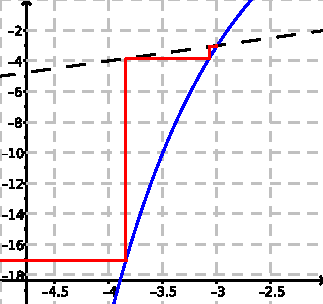
\includegraphics{figures/roots-fixedpt17}.
\par\end{center}
\begin{description}
\item [{Catatan:}] Garis $y=x$ tidak dibuat dengan sudut $45^{\circ}$
karena rasio aspek grafik bukan $1:1$. Sumbu $y$ mencakup panjang
20, dari $-20$ hingga $0$ sedangkan sumbu $x$ mencakup panjang
hanya 3, dari $-5$ hingga $-2$. 
\end{description}
\item [{\ref{exc:fixedpt-12}:}] (a) Untuk menetapkan bahwa $f$ memiliki
titik tetap tunggal pada $[-4,-.9]$, kita akan menunjukkan bahwa
$f$ kontinu pada $[-4,-.9]$, $f([-4,-.9])\subseteq[-4,-.9]$ dan
$|f'(x)|\leq1$ untuk semua $x\in(-4,-.9)$. Proposisi \ref{prop:uniquenessOfFixedPoint}
memberi kita hasil tersebut.

\begin{description}
\item [{(i)}] $f$ kontinu pada $[-4,-.9]$ karena satu-satunya diskontinuitasnya
berada di $x=-\frac{2}{3}$, tempat penyebut, $6x+4$, bernilai nol,
dan $-\frac{2}{3}\approx-.6666$ tidak berada dalam $[-4,-.9]$.
\item [{(ii)}] Kita mencari ekstrem absolut dari $f$ pada $[-4,-.9]$.
$f'(x)=\frac{18x^{2}+24x+6}{36x^{2}+48x+16}=\frac{3(x+1)(3x+1)}{2(3x+2)^{2}}$
memiliki nol di $x=-1$ dan $x=-\frac{1}{3}$ dan tidak terdefinisi
di $x=-\frac{2}{3}$. Satu-satunya nilai kritis yang relevan adalah
$-1$, sehingga kita memeriksa $f(-4)=-\frac{47}{20}=-2.35$, $f(-1)=-1$,
dan $f(-.9)=-\frac{143}{140}\approx-1.021$. Jadi, $f([-4,-.9])\subseteq[-2.35,-1]\subseteq[-4,-0.9]$.
\textbf{Catatan:} Untuk banyak fungsi, bukti visual sudah cukup memuaskan
atau setidaknya kita dapat menggunakan grafik untuk memverifikasi
kesimpulan. Dalam soal ini, grafik $f$ untuk nilai $x$ dan $y$
dari $-4$ hingga $-.9$ tampak seperti

\begin{center}
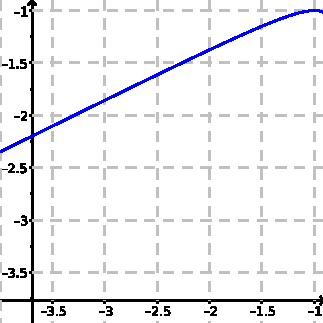
\includegraphics{figures/roots-fixedpt18}.
\par\end{center}

Grafik fungsi tidak keluar dari bidang tampilan melalui bagian atas
(tidak ada nilai yang lebih besar dari $-.9$) maupun bagian bawah
(tidak ada nilai yang kurang dari $-4$), sehingga $f([-4,-.9])\subseteq[-4,-.9]$.
\item [{(iii)}] Kita mencari ekstrem absolut dari $f'$ pada $[-4,-.9]$.
$f''(x)=\frac{3}{27x^{3}+54x^{2}+36x+8}=\frac{3}{(3x+2)^{3}}$ tidak
memiliki nol dan hanya tidak terdefinisi di $x=-\frac{2}{3}$. Tidak
ada nilai kritis yang relevan, sehingga kita memeriksa $f'(-4)=\frac{99}{200}=0.495$
dan $f'(-.9)=-\frac{51}{98}\approx-.5204$. Jadi, $-\frac{51}{98}\leq f'(x)\leq\frac{99}{200}$
untuk semua $x\in(-4,-.9)$, yang berarti $|f'(x)|\leq\frac{51}{98}<1$
untuk semua $x\in(-4,-.9)$. \textbf{Catatan:} Seperti pada pemeriksaan
(ii), bukti visual sudah cukup memuaskan atau setidaknya kita dapat
menggunakan grafik untuk memverifikasi kesimpulan. Dalam soal ini,
grafik $f'$ untuk $x\in[-4,-.9]$ dan $y\in[-1,1]$ tampak seperti

\begin{center}
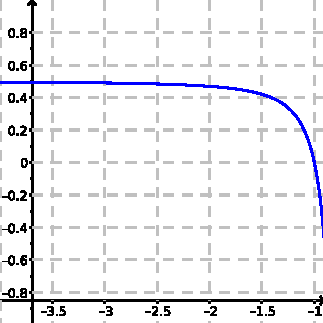
\includegraphics{figures/roots-fixedpt19}.
\par\end{center}

Grafik fungsi tidak keluar dari bidang tampilan melalui bagian atas
(tidak ada nilai yang lebih besar dari 1) maupun bagian bawah (tidak
ada nilai yang kurang dari $-1$), sehingga $|f'(x)|<1$ untuk semua
$x\in(-4,-.9)$.
\end{description}
(b) Dengan menggunakan metode iterasi titik tetap seperti dijelaskan
dalam teks dengan toleransi $10^{-2}$ dan $x_{0}=-4$, diperoleh
$x_{6}=-1.00000176319$, dan kita menganggap nilai ini akurat hingga
selisih $10^{-2}$ dari titik tetap sebenarnya. \textbf{Catatan:}
Karena kita tidak memiliki cara andal untuk menghitung galat, mungkin
saja jawaban akhir tidak berada dalam toleransi terhadap akar sebenarnya.
Namun, dalam kasus ini titik tetap sebenarnya adalah $-1$, sehingga
hasil kita berada jauh di dalam batas.
\item [{\ref{exc:fixedpt-13}:}] Pertama, $f(x)=\sqrt[3]{8-4x}=x\implies8-4x=x^{3}\implies x^{3}+4x-8=0$,
sehingga setiap titik tetap dari $f$ adalah akar dari $g$. Selanjutnya
perlu ditunjukkan bahwa metode iterasi titik tetap akan konvergen
ke titik tetap dari $f$ untuk setiap nilai awal $x_{0}\in[1.2,1.5]$.
Menurut teorema kekonvergenan titik tetap, kita perlu menetapkan bahwa
$[1.2,1.5]$ adalah lingkungan suatu titik tetap tempat magnitudo
turunannya kurang dari 1.

\begin{description}
\item [{(i)}] Untuk menetapkan bahwa terdapat titik tetap dalam $[1.2,1.5]$,
perhatikan bahwa $f$ kontinu serta bahwa $f(1.2)-1.2=\sqrt[3]{\frac{16}{5}}-1.2\approx.27>0$
dan $f(1.5)-1.5=\sqrt[3]{2}-1.5\approx-.24<0$. Teorema nilai antara
menjamin adanya nilai $c\in(1.2,1.5)$ sedemikian sehingga $f(c)-c=0$,
atau $f(c)=c$.
\item [{(ii)}] Kita perlu menetapkan bahwa magnitudo turunan $f$ kurang
dari 1 untuk semua $x\in(1.2,1.5)$. $f'(x)=-\frac{4}{3(8-4x)^{2/3}}$
dan $f''(x)=-\frac{32}{9(8-4x)^{5/3}}$. Karena $f''(x)<0$ untuk
semua $x\in(1.2,1.5)$, kita tahu bahwa $f'$ menurun pada interval
ini. Karena alasan ini dan fakta bahwa $f'(x)<0$ untuk semua $x\in(1.2,1.5)$,
kita tahu bahwa $|f'(x)|$ dibatasi oleh $|f'(1.5)|=\left|-\frac{2\sqrt[3]{2}}{3}\right|\approx.84<1$.
\end{description}
Hal ini menyelesaikan pembuktian.
\end{description}

\section*{Bagian \ref{sec:fixedptOrder}}
\begin{description}
\item [{\ref{exc:orderOfConvergence}:}] Karena tidak ada pola khusus untuk
nilai-nilai yang akan diambil oleh $n$, kita akan menyimpan keenam
nilai dalam larik. Kemudian kita akan mengiterasi larik untuk memperoleh
nilai-nilai $f$. 

\begin{verbatim}
n=[0,1,2,4,6,10];
f=@(x) (2^(2^x)-2)/(2^(2^x)+3);
i=1;
while (i<7)
  disp(f(n(i)));
  i=i+1;
end%while
\end{verbatim}

menghasilkan keluaran berikut:

\begin{verbatim}
0
 0.285714285714286
 0.736842105263158
 0.999923709546987
 1
NaN
\end{verbatim}
\begin{description}
\item [{Catatan:}] Kita dapat menghindari NaN, yang dibaca ``Bukan Angka'',
pada nilai keenam dengan menulis ulang fungsi ke bentuk yang ekuivalen
secara aljabar \texttt{f=@(x) (1-2{*}2\textasciicircum -(2\textasciicircum x))/(1+3{*}2\textasciicircum -(2\textasciicircum x));}.
Dengan satu perubahan pada program di atas, dihasilkan keluaran berikut:

\begin{verbatim}
0
 0.285714285714286
 0.736842105263158
 0.999923709546987
 1
 1
\end{verbatim}

Hal ini bekerja karena \texttt{2\textasciicircum (2\textasciicircum 10)},
yang sama dengan $2^{1024}$, menghasilkan luapan sedangkan \texttt{2\textasciicircum -(2\textasciicircum 10)},
yang sama dengan $2^{-1024}$, bernilai $0$. $2^{1024}\approx1.8(10)^{308}$
terlalu besar untuk direpresentasikan sebagai nilai titik-mengambang
standar.
\end{description}
\item [{\ref{exc:orderOfConvergence-3}:}]~

\begin{description}
\item [{(a)}] Dengan mengikuti proposisi \ref{prop:fixedPointErrorBound},
kita memerlukan galat awal dan batas magnitudo turunan dari $f$.

\begin{description}
\item [{(i)}] Yang kita ketahui tentang nilai awal, $x_{0}$, dan titik
tetap, $\hat{x}$, hanyalah keduanya berada dalam $[-4,-.9]$, sehingga
taksiran terbaik untuk galat awal adalah lebar interval. Jadi, kita
mengambil $|x_{0}-\hat{x}|=3.1$. 
\item [{(ii)}] Dalam \ref{exc:fixedpt-12} pada Bagian \ref{sec:Fixedpt},
kita telah menetapkan fakta bahwa $|f'(x)|\leq\frac{51}{98}<1$. Jadi,
kita memperoleh $M=\frac{51}{98}$.
\end{description}
Oleh karena itu, kita tahu bahwa $|x_{k}-\hat{x}|\leq3.1\cdot\left(\frac{51}{98}\right)^{k}$,
dan besaran ini harus kurang dari $10^{-11}$:
\begin{eqnarray*}
3.1\cdot\left(\frac{51}{98}\right)^{k} & < & 10^{-11}\\
\left(\frac{51}{98}\right)^{k} & < & \frac{1}{3.1(10)^{11}}\\
k\ln\left(\frac{51}{98}\right) & < & \ln\left(\frac{1}{3.1(10)^{11}}\right)\\
k & > & \frac{-\ln\left(3.1(10)^{11}\right)}{\ln\left(\frac{51}{98}\right)}\approx40.51.
\end{eqnarray*}
Jadi, 41 iterasi akan mencukupi untuk setiap nilai awal dalam $[-4,-.9]$.
\begin{description}
\item [{Catatan:}] Tanda pertidaksamaan harus berubah dari $<$ menjadi
$>$ pada langkah terakhir karena kita membagi dengan $\ln\left(\frac{51}{98}\right)$,
yang bernilai negatif. 
\end{description}
\item [{(b)}] $x_{0}=-4$,\\
$x_{1}=f(x_{0})=-2.35$,\\
$x_{2}=f(x_{1})\approx-1.541336633663366$,\\
$x_{3}=f(x_{2})\approx-1.167517670666227$,\\
$x_{4}=f(x_{3})\approx-1.028014489100897$,\\
$x_{5}=f(x_{4})\approx-1.001085950365354$,\\
$x_{6}=f(x_{5})\approx-1.00000176318809$, dan\\
$x_{7}=f(x_{6})\approx-1.000000000004663$.\\
Diperlukan 7 iterasi untuk memperoleh taksiran dalam jarak $10^{-11}$
dari titik tetap sebenarnya, $-1$.
\item [{(c)}] Batas teoretis adalah 41, sedangkan jumlah iterasi sebenarnya
adalah 7. Batas tersebut hampir enam kali nilai sebenarnya! Ini bukan
batas yang ketat.

\begin{description}
\item [{Catatan:}] Batas tersebut begitu longgar karena turunan di titik
tetap bernilai nol. Taksiran dalam proposisi \ref{prop:fixedPointErrorBound}
tidak memperhitungkan kasus ini, yang diketahui memiliki kekonvergenan
kuadratik atau lebih baik.
\end{description}
\end{description}
\item [{\ref{exc:orderOfConvergence-6}:}]~

\begin{center}
\begin{tabular}{c|cc}
$n$ & $p_{n}$ & $a_{n}$\tabularnewline
\hline 
0 & $0.5$ & $0.2586844276$\tabularnewline
1 & $0.2004262431$ & $0.2576132107$\tabularnewline
2 & $0.2727490651$ & $0.2575358323$\tabularnewline
3 & $0.2536071566$ & $0.2575306600$\tabularnewline
4 & $0.2585503763$ & $0.2575303107$\tabularnewline
5 & $0.2572656363$ & \tabularnewline
6 & $0.2575989852$ & \tabularnewline
\end{tabular}
\par\end{center}
\item [{\ref{exc:orderOfConvergence-8}:}] Iterasi kesepuluh metode Steffensen
adalah $0.01462973293$ sedangkan iterasi kesebelas adalah $0.009752946539$,
sehingga hanya diperlukan 11 iterasi untuk mencapai bilangan di bawah
$0.01$. Percepatan kekonvergenan ini luar biasa---dari $29,992$
iterasi menjadi 11. 
\end{description}

\section*{Bagian \ref{sec:newtonsMethod}}
\begin{description}
\item [{\ref{exc:newton-2}:}] Metode Newton (iterasi titik tetap) memerlukan
iterasi fungsi $f(x)=x-\frac{g(x)}{g'(x)}$, sehingga kita perlu mengetahui
$g'(x)$. Turunan dari $g$ adalah
\[
g'(x)=\text{\textminus}\frac{200\sin\left(\frac{10}{x}\right)}{x^{3}}\text{\textminus}\frac{1000\cos\left(\frac{10}{x}\right)}{x^{4}}.
\]
Oleh karena itu,
\[
x_{1}=1.25-\frac{g(1.25)}{g'(1.25)}=\frac{\frac{100}{1.25^{2}}\sin\left(\frac{10}{1.25}\right)}{\text{\textminus}\frac{200\sin\left(\frac{10}{1.25}\right)}{1.25^{3}}\text{\textminus}\frac{1000\cos\left(\frac{10}{1.25}\right)}{1.25^{4}}}\approx2.76794916279264
\]
 dan 
\[
x_{2}=x_{1}-\frac{g(x_{1})}{g'(x_{1})}=\frac{\frac{100}{x_{1}^{2}}\sin\left(\frac{10}{x_{1}}\right)}{\text{\textminus}\frac{200\sin\left(\frac{10}{x_{1}}\right)}{x_{1}^{3}}\text{\textminus}\frac{1000\cos\left(\frac{10}{x_{1}}\right)}{x_{1}^{4}}}\approx3.07240930016243.
\]

\begin{description}
\item [{Catatan:}] Meskipun tidak mutlak diperlukan dalam bentuk yang disederhanakan,
\[
f(x)=x-\frac{g(x)}{g'(x)}=\frac{3x^{2}\sin\left(\frac{10}{x}\right)+10x\cos\left(\frac{10}{x}\right)}{2x\sin\left(\frac{10}{x}\right)+10\cos\left(\frac{10}{x}\right)}.
\]
Oleh karena itu, $x_{1}=\frac{3\cdot1.25^{2}\sin\left(\frac{10}{1.25}\right)+10(1.25)\cos\left(\frac{10}{1.25}\right)}{2(1.25)\sin\left(\frac{10}{1.25}\right)+10\cos\left(\frac{10}{1.25}\right)}\approx2.76794916279264$,
dan $x_{2}$ juga dapat dihitung menggunakan ekspresi ini.
\end{description}
\item [{\ref{exc:newton-3}:}] Rumus metode sekan adalah
\[
x_{n+1}=x_{n}-g(x_{n})\frac{x_{n}-x_{n-1}}{g(x_{n})-g(x_{n-1})}.
\]
 Ketika $n=1$, diperoleh $x_{2}=x_{1}-g(x_{1})\frac{x_{1}-x_{0}}{g(x_{1})-g(x_{0})}$,
sehingga dalam contoh ini, 
\[
x_{2}=6-g(6)\frac{6-5}{g(6)-g(5)}\approx10.15086029699136.
\]
Ketika $n=2$, diperoleh $x_{3}=x_{2}-g(x_{2})\frac{x_{2}-x_{1}}{g(x_{2})-g(x_{1})}$,
sehingga dalam contoh ini,
\[
x_{3}=x_{2}-g(x_{2})\frac{x_{2}-6}{g(x_{2})-g(6)}\approx8.43462052844703.
\]
\item [{\ref{exc:newton-6}:}] Karena metode Newton merupakan metode iterasi
titik tetap, kita dapat menggunakan teorema kekonvergenan titik tetap
untuk mencari interval semacam itu. Seperti ditunjukkan dalam latihan
\ref{enu:convergenceStrengthened} \vpageref{enu:convergenceStrengthened},
kita dijamin memperoleh kekonvergenan pada setiap lingkungan akar
tempat fungsi yang diiterasikan $f$ memiliki turunan dengan magnitudo
kurang dari $1$. Untuk itu, $f(x)=x-\frac{g(x)}{g'(x)}=x-\frac{x^{4}+2x^{3}-x-3}{4x^{3}+6x^{2}-1}$.
Jadi,
\begin{eqnarray*}
f'(x) & = & 1-\frac{(4x^{3}+6x^{2}-1)^{2}-(12x^{2}+12x)(x^{4}+2x^{3}-x-3)}{(4x^{3}+6x^{2}-1)^{2}}\\
 & = & \frac{(12x^{2}+12x)(x^{4}+2x^{3}-x-3)}{(4x^{3}+6x^{2}-1)^{2}}.
\end{eqnarray*}
Grafik $f'$ di sekitar $1.097740792$,

\begin{center}
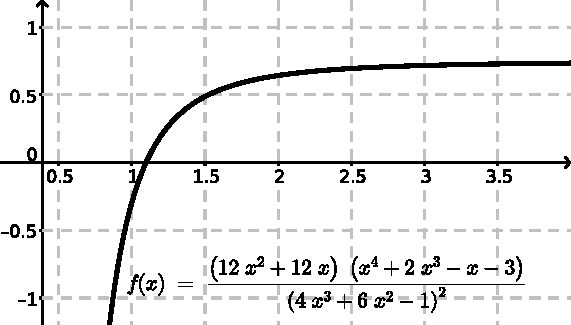
\includegraphics{figures/roots-newton5},
\par\end{center}

\noindent tampaknya menunjukkan bahwa $|f'(x)|<1$ untuk semua $x$
dari kira-kira $0.9$ hingga $\infty$. Ini jawaban yang dapat diterima,
tetapi jika kita menginginkan batas bawah yang lebih tepat dan ingin
membuktikan pernyataan tersebut, masih banyak pekerjaan yang harus
dilakukan. Pertama, akar-akar $4x^{3}+6x^{2}-1$ kira-kira adalah
$-1.4$, $-0.5$, dan $0.4$, sehingga tidak ada asimtot pada interval
yang ditinjau. $f'$ kontinu di sana. Untuk menemukan ujung bawah
interval ini, kita menyelesaikan persamaan $f'(x)=-1$:
\begin{eqnarray*}
\frac{(12x^{2}+12x)(x^{4}+2x^{3}-x-3)}{(4x^{3}+6x^{2}-1)^{2}} & = & -1\\
(12x^{2}+12x)(x^{4}+2x^{3}-x-3) & = & -(4x^{3}+6x^{2}-1)^{2}\\
12\,x^{6}+36x^{5}+24x^{4}-12x^{3}-48x^{2}-36x & = & -16x^{6}-48x^{5}-36x^{4}+8x^{3}+12x^{2}-1\\
28x^{6}+84x^{5}+60x^{4}-20x^{3}-60x^{2}-36x+1 & = & 0.
\end{eqnarray*}
Solusi riil persamaan ini, dalam urutan menurun, kira-kira adalah
$0.871748$, $0.026590$, $-1.026590$, dan $-1.871748$. Grafik $28x^{6}+84x^{5}+60x^{4}-20x^{3}-60x^{2}-36x+1$
akan memberi petunjuk yang tepat, dan metode Newton dapat digunakan
untuk mencari akar-akar tersebut. Akar yang kita cari adalah $0.871748$.
Nilai ini menandai ujung bawah interval yang diinginkan. Untuk memverifikasi
bahwa interval tersebut tak berbatas di atas, kita menyelesaikan $f'(x)=1$:
\begin{eqnarray*}
\frac{(12x^{2}+12x)(x^{4}+2x^{3}-x-3)}{(4x^{3}+6x^{2}-1)^{2}} & = & 1\\
(12x^{2}+12x)(x^{4}+2x^{3}-x-3) & = & (4x^{3}+6x^{2}-1)^{2}\\
12\,x^{6}+36x^{5}+24x^{4}-12x^{3}-48x^{2}-36x & = & 16x^{6}+48x^{5}+36x^{4}-8x^{3}-12x^{2}+1\\
0 & = & 4x^{6}+12x^{5}+12x^{4}+4x^{3}+36x^{2}+36x+1.
\end{eqnarray*}
 Solusi riil persamaan ini, dalam urutan menurun, kira-kira adalah
$-0.028593$ dan $-0.971407$. Sekali lagi, grafik akan memberi petunjuk
yang tepat, dan metode Newton dapat digunakan untuk mencari akar-akar
tersebut. Tidak ada solusi $f'(x)=\pm1$ yang lebih besar daripada
akar $1.097740792$. Kita menyimpulkan bahwa $|f'(x)|<1$ untuk semua
$x\in(0.87175,\infty)$, sehingga metode Newton akan konvergen ke
$\hat{x}\approx1.097740792$ untuk setiap nilai awal dalam $(0.87175,\infty)$.
Akhirnya, dengan melihat grafik $f(x)$,

\begin{center}
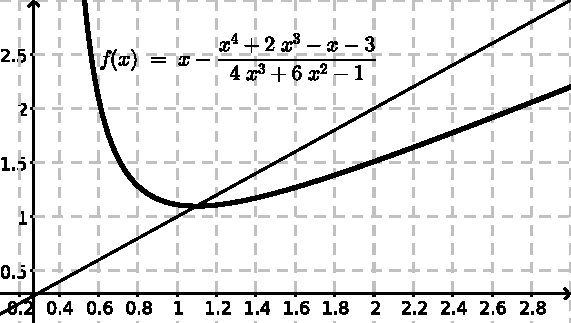
\includegraphics{figures/roots-newton6},
\par\end{center}

\noindent kita melihat bahwa interval dari asimtot di sekitar $0.4$
hingga akar dipetakan ke interval dari akar hingga tak hingga. Oleh
karena itu, metode Newton konvergen ke $1.097740792$ untuk semua
nilai awal di antara asimtot di dekat $0.4$ dan $0.87175$ juga.
Akhirnya, kita menggunakan metode Newton untuk memperoleh nilai asimtot
yang lebih akurat di dekat $0.4$. Nilainya ternyata $0.366025403784439$,
sehingga kita menyimpulkan bahwa metode Newton akan konvergen ke akar
$\hat{x}\approx1.097740792$ untuk setiap nilai awal dalam $(0.36602540378444,\infty)$.
\begin{description}
\item [{Catatan:}] Bergantung pada seberapa ketat pembuktian jawaban yang
Anda inginkan, Anda dapat memulai dengan grafik $f$ seperti di atas,
menghampiri asimtot di dekat $0.4$, lalu langsung menuju jawaban
akhir. Kesimpulan ini dapat dibenarkan secara grafis dengan mengasumsikan
bahwa grafik dari $f$ kurang lebih linear di sebelah kanan bagian
yang ditampilkan dan membayangkan diagram jaring untuk sembarang nilai
dalam interval ini. Untuk membuat argumen ini sedikit lebih ketat,
perhatikan bahwa $f$ memiliki asimtot miring, $y=\frac{3}{4}x$,
ketika $x$ mendekati $\infty$, sehingga asumsi bahwa grafik $f$
kurang lebih berupa garis lurus di sebelah kanan bagian yang ditampilkan
memang sah.
\end{description}
\item [{\ref{exc:newton-8}:}]~

\begin{center}
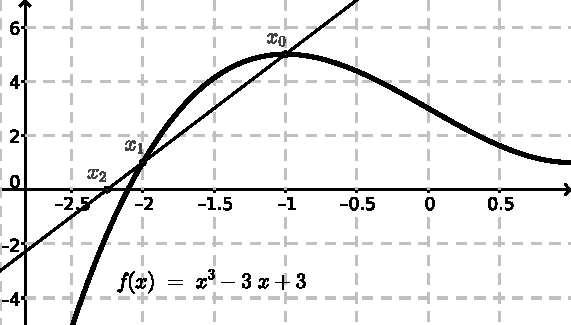
\includegraphics{figures/roots-newton7}
\par\end{center}
\item [{\ref{exc:newton-11}:}] Jumlah dua bilangan, sebutlah $x$ dan
$y$, adalah 20, sehingga $x+y=20$. Jika setiap bilangan dijumlahkan
dengan akar kuadratnya, hasil kali kedua jumlah adalah $172.2$, sehingga
$(x+\sqrt{x})(y+\sqrt{y})=172.2$. Jadi, kita perlu menyelesaikan
sistem
\begin{eqnarray*}
x+y & = & 20\\
(x+\sqrt{x})(y+\sqrt{y}) & = & 172.2
\end{eqnarray*}
dua persamaan dengan dua peubah. Karena sistem ini tidak linear, harapan
terbaik kita adalah menggunakan substitusi. Persamaan pertama memberi
kita $y=20-x$. Dengan menyubstitusikan nilai $y$ ini ke persamaan
kedua, diperoleh
\[
(x+\sqrt{x})(20-x+\sqrt{20-x})=172.2
\]
atau $(x+\sqrt{x})(20-x+\sqrt{20-x})-172.2=0$. Kita mencari solusi
persamaan terakhir ini. Tanpa gambaran mengenai akar-akarnya selain
asumsi wajar bahwa akar-akar tersebut berada di antara 0 dan 20, tidak
jelas nilai awal mana yang harus digunakan. Dengan beberapa percobaan
berbeda, kemungkinan Anda menemukan nilai yang berhasil. Sebagai contoh,
menerapkan metode sekan pada $g(x)=(x+\sqrt{x})(20-x+\sqrt{20-x})-172.2$
dengan $x_{0}=9$ dan $x_{1}=10$ menghasilkan $9.149620618$, yang
akurat hingga semua digit yang ditampilkan, hanya dalam 9 iterasi.
Bilangan lainnya adalah $20-9.149620618=10.850379382$. Kita dapat
memverifikasi bahwa ini solusi dengan menghitung
\[
(9.149620618+\sqrt{9.149620618})(10.850379382+\sqrt{10.850379382})
\]
yang sangat dekat dengan $172.2$.
\item [{\ref{exc:newton-12}:}] Metode Newton akan gagal menemukan akar
dari $g$ pada iterasi kedua jika $g'(x_{1})=0$. Sebagai contoh,
misalkan $g(x)=x^{3}-3x+3$. Kemudian $g'(x)=3x^{2}-3$ memiliki nol
ketika $x=\pm1$. Jadi, kita memerlukan nilai $x_{0}$ sedemikian
sehingga $x_{1}=1$ atau $x_{1}=-1$. Kita perlu mencari sembarang
solusi dari $x_{1}=x_{0}-\frac{g(x_{0})}{g'(x_{0})}=x-\frac{x^{3}-3x+3}{3x^{2}-3}=\pm1$.
Salah satu solusi tersebut adalah sebagai berikut. 
\begin{eqnarray*}
x-\frac{x^{3}-3x+3}{3x^{2}-3} & = & 1\\
\frac{2x^{3}-3}{3x^{2}-3} & = & 1\\
2x^{3}-3 & = & 3x^{2}-3\\
2x^{3}-3x^{2} & = & 0\\
x^{2}(2x-3) & = & 0
\end{eqnarray*}
sehingga salah satu nilai awal $x_{0}=0$ atau $x_{0}=\frac{3}{2}$
akan memberikan hasil yang diinginkan.

\begin{description}
\item [{Catatan:}] Persamaan $x-\frac{x^{3}-3x+3}{3x^{2}-3}=-1$ hanya
memiliki satu solusi riil, tetapi solusi tersebut irasional. Hingga
20 angka signifikan, nilainya adalah $1.0786168885087585968$. Menetapkan
$x_{0}=1.078616888508759$ seperti dalam kode Octave berikut ternyata
tidak menyebabkan kegagalan! Terdapat cukup banyak galat pembulatan
sehingga $x_{1}$ tidak persis sama dengan $-1$ dan $g'(x_{1})$
tidak persis nol, sehingga metode tetap berjalan dan menemukan hasilnya.
Diperlukan 99 iterasi untuk mendekati solusi secara stabil, tetapi
akhirnya tercapai. $x_{1}$ ditampilkan sebagai \texttt{-0.999999999999999}
dan $x_{2}$ ditampilkan sebagai \texttt{7.50599937895082e+14}.
\end{description}
\begin{verbatim}
format('long')
f=@(x) x^3-3*x+3
fp=@(x) 3*x^2-3
x0=1.0786168885087585968
c=1;
for i=1:120
  x=x0-f(x0)/fp(x0)
  if (abs(x-x0)<1e-15)
    c
    return
  end%if
  x0=x;
  c=c+1;
end%for
\end{verbatim}
\end{description}

\section*{Bagian \ref{sec:moreConvergenceDiagrams}}
\begin{description}
\item [{\ref{exc:more}:}] Sebelum mencocokkan fungsi dengan diagramnya,
kita periksa fungsi-fungsi yang tersedia. $f$ dan $h$ adalah polinom
derajat 5 dan karena itu memiliki paling banyak 5 akar berbeda. $l$
adalah hasil kali logaritma alami dengan polinom derajat tiga. Polinom
tersebut memiliki tiga akar dan logaritmanya memiliki satu akar yang
berbeda dari akar-akar polinom, sehingga $l$ memiliki empat akar.
Sekarang, dengan melihat diagram, kita dapat mencocokkan dua fungsi
dengan diagramnya. Diagram (d) memiliki bidang dengan sembilan warna
berbeda, yang menunjukkan sembilan akar dalam daerah yang ditampilkan.
Karena fungsi $f$, $h$, dan $l$ memiliki kurang dari 9 akar, fungsi
$g$ pasti cocok dengan diagram (d). Dengan penalaran serupa, diagram
(a) dan (b) sama-sama menunjukkan 5 akar, sehingga $l$ tidak dapat
cocok dengan salah satunya. $l$ hanya memiliki empat akar. Dengan
proses eliminasi, fungsi $l$ cocok dengan diagram (c). Dengan demikian,
diagram (a) dan (b) tersisa untuk dicocokkan dengan $f$ dan $h$.
Kedua diagram menunjukkan 5 akar, tetapi terdapat perbedaan mendasar
di antara keduanya. Sumbu riil melintas secara horizontal melalui
pusat setiap diagram. Diagram (a) memiliki satu bidang yang menutupi
seluruh sumbu riil, yang menunjukkan hanya satu akar riil, sedangkan
diagram (b) memiliki tiga bidang yang menutupi sumbu riil, yang menunjukkan
tiga akar riil. Grafik $f$,

\begin{center}
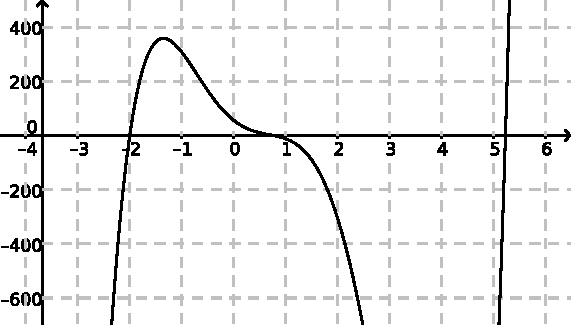
\includegraphics{figures/roots-more3},
\par\end{center}

dengan jelas menunjukkan bahwa $f$ memiliki tiga akar, sehingga $f$
cocok dengan (b) dan $h$ cocok dengan (a). Ringkasnya,
\begin{eqnarray*}
f & \leftrightarrow & \mbox{(b)}\\
g & \leftrightarrow & \mbox{(d)}\\
h & \leftrightarrow & \mbox{(a)}\\
l & \leftrightarrow & \mbox{(c)}.
\end{eqnarray*}

\item [{\ref{exc:more-2}:}] Untuk setiap akar $r$, polinom harus memiliki
faktor $(x-r)$ dan tidak memiliki faktor lain. Polinom ini harus
memiliki faktor $(x-(-4))$, $(x-(-1))$, $(x-2)$, $(x-2i)$, dan
$(-(-2i))$, sehingga $p(x)=(x+4)(x+1)(x-2)(x-2i)(x+2i)$ merupakan
salah satu solusi.

\begin{description}
\item [{Catatan:}] $q(x)=a(x+4)(x+1)(x-2)(x-2i)(x+2i)$ dengan $a$ berupa
sembarang bilangan kompleks tak nol juga merupakan solusi.
\item [{Catatan:}] Meskipun faktor-faktornya tidak perlu dikalikan, $p(x)=x^{5}+3x^{4}\text{\textminus}2x^{3}+4x^{2}\text{\textminus}24x\text{\textminus}32$.
\end{description}
\item [{\ref{exc:more-4}:}] Untuk setiap akar $r$, polinom harus memiliki
faktor $(x-r)$ dan tidak memiliki faktor lain. Polinom ini harus
memiliki faktor $(x-(-4))$, $(x-(-1))$, $(x-2)$, dan $(x-2i)$,
sehingga $p(x)=(x+4)(x+1)(x-2)(x-2i)$ merupakan salah satu solusi.

\begin{description}
\item [{Catatan:}] $q(x)=a(x+4)(x+1)(x-2)(x-2i)$ dengan $a$ berupa sembarang
bilangan kompleks tak nol juga merupakan solusi.
\item [{Catatan:}] Meskipun faktor-faktornya tidak perlu dikalikan, $p(x)=x^{4}+(3-2i)x^{3}-(6+6i)x^{2}-(8-12i)x+16i$.
Perhatikan bahwa tidak semua koefisiennya merupakan bilangan riil.
Hal ini konsisten dengan teorema akar konjugat yang menyatakan bahwa
jika polinom dengan koefisien riil memiliki akar kompleks, akar-akar
tersebut harus muncul dalam pasangan konjugat.
\end{description}
\item [{\ref{exc:more-3}:}] $f$ bersifat periodik dan memiliki tak hingga
banyak akar yang tersebar teratur di sepanjang sumbu riil. Satu-satunya
diagram yang menunjukkan akar semacam ini adalah (a), sehingga $f$
cocok dengan (a). $g$ dan $f$ hanya berbeda sedikit untuk nilai
riil yang besar, sehingga kita mengharapkan tak hingga banyak akar
yang kurang lebih berjarak teratur pada sumbu riil positif. Satu-satunya
diagram dengan akar semacam ini adalah (d), sehingga $g$ cocok dengan
(d). $l$ adalah polinom derajat lima, sehingga memiliki paling banyak
5 akar. Diagram (b) menunjukkan 8 warna, sehingga terdapat 8 akar.
Oleh karena itu, $h$ cocok dengan (b) dan $l$ cocok dengan (c).
Ringkasnya,
\begin{eqnarray*}
f & \leftrightarrow & \mbox{(a)}\\
g & \leftrightarrow & \mbox{(d)}\\
h & \leftrightarrow & \mbox{(b)}\\
l & \leftrightarrow & \mbox{(c)}.
\end{eqnarray*}
\end{description}

\section*{Bagian \ref{sec:RootsOfPolynomials}}
\begin{description}
\item [{\ref{exc:polynomials-6}:}] $g(2)=38$ dan $g'(2)=71$:

\begin{center}
\begin{tabular}{ccccc}
\multicolumn{1}{c|}{$2$} & $3$ & $12$ & $-13$ & $-8$\tabularnewline
\cline{1-1}
 &  & $6$ & $36$ & $46$\tabularnewline
\cline{2-5}
\multicolumn{1}{c|}{$2$} & $3$ & $18$ & \multicolumn{1}{c|}{$23$} & \multicolumn{1}{c|}{$38$}\tabularnewline
\cline{1-1}\cline{5-5}
 &  & $6$ & $48$ & \tabularnewline
\cline{2-5}
 & $3$ & \multicolumn{1}{c|}{$24$} & \multicolumn{1}{c|}{$71$} & \tabularnewline
\cline{4-4}
\end{tabular}
\par\end{center}
\item [{\ref{exc:polynomials-10}a:}] Dari \ref{exc:polynomials-6}, $g(2)=38$
dan $g'(2)=71$, sehingga $x_{1}=2-\frac{38}{71}=\frac{104}{71}$.
$g(\frac{104}{71})=\frac{2911104}{357911}$ dan $g'(\frac{104}{71})=\frac{209027}{5041}$:

\begin{center}
\setlength{\extrarowheight}{5pt}%
\begin{tabular}{ccccc}
\multicolumn{1}{c|}{$\frac{104}{71}$} & $3$ & $12$ & $-13$ & $-8$\tabularnewline
\cline{1-1}
 &  & $\frac{312}{71}$ & $\frac{121056}{5041}$ & $\frac{5774392}{357911}$\tabularnewline
\cline{2-5}
\multicolumn{1}{c|}{$\frac{104}{71}$} & $3$ & $\frac{1164}{71}$ & \multicolumn{1}{c|}{$\frac{55523}{5041}$} & \multicolumn{1}{c|}{$\frac{2911104}{357911}$}\tabularnewline
\cline{1-1}\cline{5-5}
 &  & $\frac{312}{71}$ & $\frac{153504}{5041}$ & \tabularnewline
\cline{2-5}
 & $3$ & \multicolumn{1}{c|}{$\frac{1476}{71}$} & \multicolumn{1}{c|}{$\frac{209027}{5041}$} & \tabularnewline
\cline{4-4}
\end{tabular}
\par\end{center}

sehingga $x_{2}=\frac{104}{71}-\frac{2911104/357911}{209027/5041}=\frac{2689672}{2120131}\approx1.268634815490175$.
\item [{\ref{exc:polynomials-5}:}] \texttt{newtonhorner({[}-144,144,-59,6,1{]},1,1e-5,100)}
mengembalikan \texttt{ans = 3}.

\begin{center}
\begin{tabular}{cccccc}
\multicolumn{1}{c|}{$3$} & $1$ & $6$ & $-59$ & $144$ & $-144$\tabularnewline
\cline{1-1}
 &  & $3$ & $27$ & $-96$ & $144$\tabularnewline
\cline{2-6}
 & $1$ & $9$ & $-32$ & \multicolumn{1}{c|}{$48$} & \multicolumn{1}{c|}{$0$}\tabularnewline
\cline{6-6}
\end{tabular}
\par\end{center}

sehingga polinom hasil deflasi adalah $x^{3}+9x^{2}-32x+48$. \texttt{newtonhorner({[}48,-32,9,1{]},3,1e-5,100)}
mengembalikan \texttt{ans = -12}.

\begin{center}
\begin{tabular}{ccccc}
\multicolumn{1}{c|}{$-12$} & $1$ & $9$ & $-32$ & $48$\tabularnewline
\cline{1-1}
 &  & $-12$ & $36$ & $-48$\tabularnewline
\cline{2-5}
 & $1$ & $-3$ & \multicolumn{1}{c|}{$4$} & \multicolumn{1}{c|}{$0$}\tabularnewline
\cline{5-5}
\end{tabular}
\par\end{center}

sehingga polinom hasil deflasi adalah $x^{2}-3x+4$ yang merupakan
polinom kuadrat. Rumus kuadrat menghasilkan akar-akar lainnya, $\frac{3\pm\sqrt{9-4(4)}}{2}=\frac{3+i\sqrt{7}}{2}$
dan $\frac{3-i\sqrt{7}}{2}$. Ringkasnya, keempat akar tersebut adalah
$3,-12,\frac{3+i\sqrt{7}}{2},\frac{3-i\sqrt{7}}{2}$.
\item [{\ref{exc:polynomials-16}:}] \texttt{format('long'); c={[}-40,16,-12,-2,1{]};
newtonhorner(c,1,1e-5,100)} mengembalikan 

\begin{center}
\texttt{ans = -3.54823289798023}
\par\end{center}

sehingga $-3.54823289798023$ adalah salah satu akar. \texttt{c=deflate(c,ans)}
mengembalikan \begin{verbatim}
c =

  -11.27321716194279   7.68642249426964  -5.54823289798023   1.00000000000000
\end{verbatim} sehingga polinom hasil deflasi kira-kira adalah $x^{3}-5.5482x^{2}+7.6864x-11.2732$
dan koefisien polinom ini kini tersimpan dalam larik \texttt{c}. \texttt{newtonhorner(c,-3.5,1e-5,100)}
mengembalikan \texttt{ans = 4.38111344099655} sehingga $4.38111344099655$
adalah akar lainnya. \texttt{c=deflate(c,ans)} mengembalikan \begin{verbatim}
c =

   2.57313975402986  -1.16711945698368   1.00000000000000
\end{verbatim} sehingga polinom hasil deflasi kira-kira adalah $x^{2}-1.1671x+2.5731$
dan koefisien polinom ini kini tersimpan dalam larik \texttt{c}. Karena
polinom telah dideflasi menjadi polinom kuadrat, kita mencari dua
akar terakhir dengan rumus kuadrat. \texttt{{[}s,t{]}=quadraticRoots(c(3),c(2),c(1))}
mengembalikan \begin{verbatim}
s =  0.583559728491838 + 1.494188006012761i
t =  0.583559728491838 - 1.494188006012761i.
\end{verbatim} Ringkasnya, akar-akarnya adalah 
\[
\begin{gathered}-3.54823289798023\\
4.38111344099655\\
0.583559728491838+1.494188006012761i\\
0.583559728491838-1.494188006012761i.
\end{gathered}
\]

\item [{\ref{exc:polynomials-18}a:}] \texttt{c={[}-40,16,-12,-2,1{]};
newtonhorner(c,-3.54823289798023,1e-5,100)}

\begin{center}
mengembalikan 
\par\end{center}

\texttt{ans = -3.54823289797970}.

\texttt{c={[}-40,16,-12,-2,1{]}; newtonhorner(c,4.38111344099655,1e-5,100)}

\begin{center}
mengembalikan 
\par\end{center}

\texttt{ans = 4.38111344099594}.

\texttt{c={[}-40,16,-12,-2,1{]}; newtonhorner(c,0.583559728491838+1.494188006012761i,1e-5,100)}

\begin{center}
mengembalikan 
\par\end{center}

\texttt{ans = 0.583559728491879 + 1.494188006011256i}.

\texttt{c={[}-40,16,-12,-2,1{]}; newtonhorner(c,0.583559728491838-1.494188006012761i,1e-5,100)}

\begin{center}
mengembalikan 
\par\end{center}

\texttt{ans = 0.583559728491879 - 1.494188006011256i}.

Setiap upaya menyempurnakan akar menghasilkan jawaban yang sedikit
berbeda, tetapi tidak ada yang berubah pada lima angka desimal pertama.
Semua akar hampiran dari polinom hasil deflasi hampiran berada dalam
jarak paling jauh $10^{-5}$ dari akar eksak polinom asli tanpa penyempurnaan.
\item [{\ref{exc:polynomials-8}:}] (i) \texttt{format('long'); horner(sqrt(3),{[}-40,16,-12,-2,1{]})}
mengembalikan \texttt{ans = -49.6794919243112}. Perhatikan bahwa kita
hanya memperoleh nilai polinom, yaitu entri pertama dari larik nilai
kembalian. Ini merupakan perilaku bawaan jika fungsi tidak disetarakan
dengan sebuah larik.

(ii) \texttt{p=@(x) x\textasciicircum 4-2{*}x\textasciicircum 3-12{*}x\textasciicircum 2+16{*}x-40;
p(sqrt(3))} mengembalikan \texttt{ans = -49.6794919243112} sehingga
keduanya tampak mengembalikan nilai yang sama.

(iii) \texttt{horner(sqrt(3),{[}-40,16,-12,-2,1{]}) == p(sqrt(3))}
mengembalikan \texttt{ans = 0}, tetapi secara internal hasilnya ternyata
tidak persis sama! Kita dapat menyimpulkan bahwa penghitungan nilai
fungsi anonim tidak dilakukan dengan penyarangan (pembagian sintetis).
\begin{description}
\item [{Catatan:}] \texttt{horner(3,{[}-40,16,-12,-2,1{]}) == p(3)} mengembalikan
\texttt{ans = 1}, jadi untuk masukan bilangan bulat 3, kedua metode
memang menghasilkan nilai yang persis sama.
\end{description}
\end{description}

\section*{Bagian \ref{sec:RootsBracketing}}
\begin{description}
\item [{\ref{exc:bracketing}:}] (c) $g(a)=g(0)=2$ dan $g(b)=g(.9)=-.1897$
sehingga selang pengurungnya sah. Selain itu, kini kita tahu bahwa
jika nilai fungsi positif pada suatu iterasi, iterasi tersebut menjadi
titik ujung kiri. Jika tidak, iterasi tersebut menjadi titik ujung
kanan. Ingat, metode sekan yang diterapkan pada selang pengurung yang
sah selalu menghasilkan iterasi di dalam selang pengurung, sehingga
metode bagi dua tidak pernah diperlukan.

\begin{center}
\begin{tabular}{cccccc}
$a$ & $b$ & kandidat $x$ & $x$ & $g(x)$ & $x$ menjadi\tabularnewline
\hline 
$0$ & $0.9$ & $0.82203$ & $0.82203$ & $-0.207$ & $b$\tabularnewline
$0$ & $0.82203$ & $0.74486$ & $0.74486$ & $-0.137$ & $b$\tabularnewline
$0$ & $0.74486$ & $0.69690$ & $0.69690$ & $-0.060$ & $b$\tabularnewline
$0$ & $0.69690$ & $0.67660$ & $0.67660$ & $-0.020$ & $b$\tabularnewline
$0$ & $0.67660$ & $0.66971$ &  &  & \tabularnewline
\end{tabular}
\par\end{center}

$|.66971-.67660|=.00689<.01$ sehingga kita berhenti pada $x_{5}=.66971$.

(h) $f(a)=f(-20)\approx20$ dan $f(b)=f(20)\approx-17$ sehingga selang
pengurungnya sah. Selain itu, kini kita tahu bahwa jika nilai fungsi
positif pada suatu iterasi, iterasi tersebut menjadi titik ujung kiri.
Jika tidak, iterasi tersebut menjadi titik ujung kanan. Ingat, metode
sekan yang diterapkan pada selang pengurung yang sah selalu menghasilkan
iterasi di dalam selang pengurung, sehingga metode bagi dua tidak
pernah diperlukan.

\begin{center}
\begin{tabular}{cccccc}
$a$ & $b$ & kandidat $x$ & $x$ & $g(x)$ & $x$ menjadi\tabularnewline
\hline 
$20$ & $-20$ & $1.5262$ & $1.5262$ & $1.18$ & $a$\tabularnewline
$1.5262$ & $-20$ & $2.7013$ & $2.7013$ & $-1.16$ & $b$\tabularnewline
$1.5262$ & $2.7013$ & $2.1186$ & $2.1186$ & $0.229$ & $a$\tabularnewline
$2.1186$ & $2.7013$ & $2.2142$ & $2.2142$ & $0.011$ & $a$\tabularnewline
$2.2142$ & $2.7013$ & $2.2189$ &  &  & \tabularnewline
\end{tabular}
\par\end{center}

$|2.2189-2.2142|=.0047<.01$ sehingga kita berhenti pada $x_{5}=2.2189$.
\item [{\ref{exc:bracketing-1}:}] (c) $g(a)=g(0)=2$ dan $g(b)=g(.9)=-.1897$
sehingga selang pengurungnya sah. Selain itu, kini kita tahu bahwa
jika nilai fungsi positif pada suatu iterasi, iterasi tersebut menjadi
titik ujung kiri. Jika tidak, iterasi tersebut menjadi titik ujung
kanan. Tanda $^{*}$ menunjukkan bahwa metode bagi dua digunakan karena
kandidat jatuh di luar selang pengurung.

\begin{center}
\begin{tabular}{cccccc}
$a$ & $b$ & kandidat $x$ & $x$ & $g(x)$ & $x$ menjadi\tabularnewline
\hline 
$0$ & $0.9$ & $1.1136$ & $0.45^{*}$ & $0.59$ & $a$\tabularnewline
$0.45$ & $0.9$ & $0.63925$ & $0.63925$ & $0.060$ & $a$\tabularnewline
$0.63925$ & $0.9$ & $0.66547$ & $0.66547$ & $0.0025$ & $a$\tabularnewline
$0.66547$ & $0.9$ & $0.66666$ &  &  & \tabularnewline
\end{tabular}
\par\end{center}

$|.66666-.66547|=.00119<.01$ sehingga kita berhenti pada $x_{4}=.66666$.

(h) $f(a)=f(-20)\approx20$ dan $f(b)=f(20)\approx-17$ sehingga selang
pengurungnya sah. Selain itu, kini kita tahu bahwa jika nilai fungsi
positif pada suatu iterasi, iterasi tersebut menjadi titik ujung kiri.
Jika tidak, iterasi tersebut menjadi titik ujung kanan. Tanda $^{*}$
menunjukkan bahwa metode bagi dua digunakan karena kandidat jatuh
di luar selang pengurung.

\begin{center}
\begin{tabular}{cccccc}
$a$ & $b$ & kandidat $x$ & $x$ & $g(x)$ & $x$ menjadi\tabularnewline
\hline 
$20$ & $-20$ & $1062.3$ & $0^{*}$ & $1$ & $a$\tabularnewline
$0$ & $-20$ & $undefined$ &  &  & \tabularnewline
\end{tabular}
\par\end{center}

Metode tersebut tak terdefinisi setelah titik ini akibat pembagian
dengan nol. Metode tersebut gagal.
\begin{description}
\item [{CATATAN:}] Kelak kita akan melihat (soal \ref{exc:bracketing-5}h)
bahwa Octave mampu menangani pembagian dengan nol dengan cukup baik
sehingga metode tersebut \textit{tetap} berlanjut dan akhirnya mencapai
solusi!
\end{description}
\item [{\ref{exc:bracketing-2}:}] (c) Metode sekan menghasilkan barisan
hampiran
\[
\begin{gathered}0,\ .9,\ .82203,\ 1.7456,\ .83551,\ .84905,\ -1.6288,\ .83478,\\
.82068,,\ .14336,\ .74168,\ .69475,\ .66071,\ .66700
\end{gathered}
\]
dan berhenti pada titik tersebut karena $|.66700-.66071|=.00629<.01$.
Metode sekan (murni) memerlukan waktu jauh lebih lama untuk konvergen
daripada versi terkurungnya. Hal ini terutama karena pada metode sekan,
iterasi ketiga berasal dari metode sekan yang diterapkan pada $.9$
dan $.82203$, yakni dua iterasi terakhir (yang tidak membentuk selang
pengurung yang sah), sedangkan iterasi ketiga pada metode posisi palsu
berasal dari metode sekan yang diterapkan pada $0$ dan $.82203$
(suatu selang pengurung yang sah).

(h) Metode sekan menghasilkan barisan hampiran
\[
-20,\ 20,\ 1.5262,\ 2.7013,\ 2.1186,\ 2.2142,\ 2.2192
\]
dan berhenti pada titik tersebut karena $|2.2192-2.2142|=.005<.01$.
Metode sekan (murni) dan versi terkurungnya menghasilkan barisan iterasi
yang persis sama. Kebetulan, pada setiap langkah, metode sekan menghasilkan
suatu hampiran, yang jika dipasangkan dengan iterasi sebelumnya membentuk
selang pengurung yang sah!
\item [{\ref{exc:bracketing-3}:}] (c) Metode Newton menghasilkan barisan
hampiran
\[
.9,\ 1.1136,\ 1.0302,\ 1.0030,\ 1.0000
\]
dan berhenti pada titik tersebut karena $|1-1.003|=.003<.01$. Metode
Newton (murni) konvergen ke akar lain, yaitu akar di luar selang pengurung!
Metode ini cepat, tetapi gagal menghasilkan akar di antara $0$ dan
$.9$, hal yang tidak mengherankan dari metode tak berpengaman.

(h) Metode Newton menghasilkan barisan hampiran
\[
\begin{gathered}20,\ 1062.3,\ 3803.0,\ 971.14,\ 377.14,\ 2880.5,\ 1606.3,\ 330.83,\ 66.635,\ 20.301,\\
-5.5823,\ -21.983,\ -10.454,\ -4.6688,\ 1.9357,\ 2.2550,\ 2.2193,\ 2.2191
\end{gathered}
\]
dan berhenti pada titik tersebut karena $|2.2191-2.2193|=.0002<.01$.
Metode Newton (murni) memerlukan waktu jauh lebih lama untuk konvergen
daripada versi terkurungnya! Metode Newton dibiarkan berkelana dengan
pola yang tampaknya acak sebelum cukup dekat dengan akar untuk berkonvergensi.
Pengurungan memaksa iterasi mendekati interval tempat metode Newton
akan konvergen dengan jauh lebih cepat.
\end{description}
\begin{enumerate}
\item \label{exc:bracketing-12}Gunakan metode sekan terkurung (posisi palsu)
untuk mencari akar dalam interval yang ditunjukkan, akurat hingga
$10^{-2}$.

\begin{enumerate}
\item $f(x)=3-x-\sin x$; $[2,3]$ \hasananswer 
\item $g(x)=3x^{4}-2x^{3}-3x+2$; $[0,1]$
\item $g(x)=3x^{4}-2x^{3}-3x+2$; $[0,0.9]$ \hasasolution 
\item $h(x)=10-\cosh(x)$; $[-3,-2]$
\item $f(t)=\sqrt{4+5\sin t}-2.5$; $[-600,-500]$ \hasananswer 
\item $g(t)=\frac{3t^{2}\tan t}{1-t^{2}}$; $[3490,3491]$
\item $h(t)=\ln(3\sin t)-\frac{3t}{5}$; $[1,2]$
\item $f(r)=e^{\sin r}-r$; $[-20,20]$ \hasasolution 
\item $g(r)=\sin(e^{r})+r$; $[-3,3]$
\item $h(r)=2^{\sin r}-3^{\cos r}$; $[1,3]$ \hasananswer 
\end{enumerate}
\end{enumerate}
\begin{description}
\item [{\ref{exc:bracketing-4}:}] (c) \begin{verbatim}
>> f2=@(x) 3*x^4-2*x^3-3*x+2;
>> [res,i]=falsePosition(f2,0,.9,10^-6,100)
b =  0.900000000000000
b =  0.822030415125360
b =  0.744866113620209
b =  0.696903242045358
b =  0.676602659540989
b =  0.669712929388636
b =  0.667578776723430
b =  0.666937771712738
b =  0.666747069128180
b =  0.666690496216585
b =  0.666673727853602
b =  0.666668758921090
b =  0.666667286598371

res =  0.666666850350527
i =  13
\end{verbatim}sehingga $x_{13}=0.666666850350527$ diperkirakan berjarak paling
jauh $10^{-6}$ dari akar sebenarnya.

(h) \begin{verbatim}
>> f7=@(r) exp(sin(r))-r;
>> [res,i]=falsePosition(f7,-20,20,10^-6,100)
b =  20
b =  1.52625394347853
b =  2.70134274226916
b =  2.11862078217644
b =  2.21421804475756
b =  2.21893051185485
b =  2.21910087293432
b =  2.21910692606145

res =  2.21910714100071
i =  8
\end{verbatim}sehingga $x_{8}=2.21910714100071$ diperkirakan berjarak paling jauh
$10^{-6}$ dari akar sebenarnya.
\item [{\ref{exc:bracketing-5}:}] (c) \begin{verbatim}
>> f2=@(x) 3*x^4-2*x^3-3*x+2;
>> f2p=@(x) 12*x^3-6*x^2-3;
>> [res,i]=bracketedNewton(f2,f2p,0,.9,10^-6,100)
b =  0.900000000000000
b =  0.450000000000000
b =  0.639257968925196
b =  0.665474256136936
b =  0.666663994320019
b =  0.666666666653136

res =  0.666666666666667
i =  6
\end{verbatim}sehingga $x_{6}=0.666666666666667$ diperkirakan berjarak paling jauh
$10^{-6}$ dari akar sebenarnya.

(h) \begin{verbatim}
>> f7=@(r) exp(sin(r))-r;
>> f7p=@(r) exp(sin(r))*cos(r)-1;
>> [res,i]=bracketedNewton(f7,f7p,-20,20,10^-6,100)
b =  20
b = 0
warning: division by zero
b =  10
b =  3.66539525575696
b =  1.65966535497164
b =  2.50454805267468
b =  2.22298743934113
b =  2.21911019802387
b =  2.21910714891565

res =  2.21910714891375
i =  9
\end{verbatim}sehingga $x_{9}=2.21910714891375$ diperkirakan berjarak paling jauh
$10^{-6}$ dari akar sebenarnya.
\begin{description}
\item [{CATATAN:}] Ketika kita mencoba menghitung solusi ini secara manual
(soal \ref{exc:bracketing-1}h), kita berhenti setelah iterasi pertama
akibat pembagian dengan nol. Namun, Octave melanjutkan dengan memperlakukan
taksiran yang tak terdefinisi sebagai taksiran yang jatuh di luar
selang pengurung. Dengan demikian, iterasi kedua adalah $10$ (metode
bagi dua yang diterapkan pada $[0,20]$).
\end{description}
\item [{\ref{exc:bracketing-6}:}] (c) \begin{verbatim}
>> f2=@(x) 3*x^4-2*x^3-3*x+2;
>> [res,i]=bracketedInverseQuadratic(f2,0,.9,10^-6,100)
b =  0.900000000000000
b =  0.822030415125360
b =  0.411015207562680
b =  0.729556813485380
b =  0.629464108906733
b =  0.671561434924253
b =  0.666977335665865
b =  0.666666168461076

res =  0.666666666960237
i =  8
\end{verbatim}sehingga $x_{8}=0.666666666960237$ diperkirakan berjarak paling jauh
$10^{-6}$ dari akar sebenarnya.

(h) \begin{verbatim}
>> f7=@(r) exp(sin(r))-r;
>> [res,i]=bracketedInverseQuadratic(f7,-20,20,10^-6,100)
b =  20
b =  1.52625394347854
b =  2.70134274226916
b =  2.11862078217644
b =  2.21421804475756
b =  2.21917736990638
b =  2.21910707796098

res =  2.21910714891272
i =  7
\end{verbatim}sehingga $x_{7}=2.21910714891272$ diperkirakan berjarak paling jauh
$10^{-6}$ dari akar sebenarnya.
\item [{\ref{exc:bracketing-9}:}] (c) \begin{verbatim}
>> f2=@(x) 3*x^4-2*x^3-3*x+2;
>> g2=@(x) f2(x)+x;
>> [res,i]=bracketedSteffensens(g2,0,.9,10^-6,100)
b =  0.900000000000000
b =  0.559577120523157
b =  0.707986331365555
b =  0.669737865924576
b =  0.666686284030401
b =  0.666666667476795

res =  0.666666667666825
i =  6
\end{verbatim}sehingga $x_{6}=0.666666667666825$ diperkirakan berjarak paling jauh
$10^{-6}$ dari akar sebenarnya.

(h) \begin{verbatim}
>> f7=@(r) exp(sin(r))-r;
>> g7=@(x) f7(x)+x;
>> [res,i]=bracketedSteffensens(g7,-20,20,10^-6,100)
b =  20
b =  1.80564417969925
b =  2.18151287547235
b =  2.21873144340028
b =  2.21910711013891

res =  2.21910707929096
i =  5
\end{verbatim}sehingga $x_{5}=2.21910707929096$ diperkirakan berjarak paling jauh
$10^{-6}$ dari akar sebenarnya.
\item [{\ref{exc:bracketing-11}:}] (c) \begin{verbatim}
>> f2=@(x) 3*x^4-2*x^3-3*x+2;
>> [res,i]=bracketedInverseQuadraticRE(f2,0,.9,10^-6,100)
b =  0.900000000000000
b =  0.822030415125360
b =  0.411015207562680
b =  0.729556813485380
b =  0.629464108906733
b =  0.671561434924253
b =  0.666977335665865
b =  0.666666168461076

res =  0.666666666960237
i =  8
\end{verbatim}sehingga $x_{8}=0.666666666960237$ diperkirakan berjarak paling jauh
$10^{-6}$ dari akar sebenarnya.

(h) \begin{verbatim}
>> f7=@(r) exp(sin(r))-r;
>> [res,i]=bracketedInverseQuadraticRE(f7,-20,20,10^-6,100)
b =  20
b =  1.52625394347854
b =  2.70134274226916
b =  2.11862078217644
b =  2.21421804475756
b =  2.21917736990638
b =  2.21910707796098

res =  2.21910714891272
i =  7
\end{verbatim}sehingga $x_{7}=2.21910714891272$ diperkirakan berjarak paling jauh
$10^{-6}$ dari akar sebenarnya.
\end{description}

\section*{Bagian \ref{sec:polynomialLagrange}}
\begin{description}
\item [{\ref{exc:interpolation-lagrange-8}:}] Kita mulai dengan membentuk
tiga polinom---polinom pertama berakar pada dua titik data terakhir
dan bernilai $1$ pada titik pertama, polinom kedua berakar pada titik
data pertama dan ketiga serta bernilai $1$ pada titik kedua, dan
polinom ketiga berakar pada titik data pertama dan kedua serta bernilai
$1$ pada titik ketiga. Polinom-polinom tersebut adalah
\begin{eqnarray*}
l_{1}(x) & = & \frac{(x-20)(x-1019)}{(-10-20)(-10-1019)}\\
l_{2}(x) & = & \frac{(x+10)(x-1029)}{(20+10)(20-1029)}\\
l_{3}(x) & = & \frac{(x+10)(x-20)}{(1019+10)(1019-20)}.
\end{eqnarray*}
Kemudian kita mengalikan $l_{i}$ dengan $y_{i}$ dan menjumlahkan
hasil kalinya:
\begin{eqnarray*}
P_{2}(x) & = & \frac{(x-20)(x-1019)}{(-10-20)(-10-1019)}(10)+\frac{(x+10)(x-1019)}{(20+10)(20-1019)}(58)\\
 &  & \qquad+\frac{(x+10)(x-20)}{(1019+10)(1019-20)}(-32).
\end{eqnarray*}
\item [{\ref{exc:interpolation-lagrange-7}c:}] Menaksir (atau menghampiri)
nilai suatu fungsi $f$ menggunakan polinom interpolasi berarti mengevaluasi
polinom tersebut di titik itu sebagai gantinya. 
\begin{eqnarray*}
f(1.3) & \approx & P_{2}(1.3)=\frac{(1.3-20)(1.3-1019)}{(-10-20)(-10-1019)}(10)+\frac{(1.3+10)(1.3-1019)}{(20+10)(20-1019)}(58)\\
 &  & \qquad+\frac{(1.3+10)(1.3-20)}{(1019+10)(1019-20)}(-32)\\
 & \approx & 28.427
\end{eqnarray*}
\item [{\ref{exc:interpolation-lagrange-2}c:}] Metode Neville paling baik
dijalankan pada komputer atau dalam format tabel. $f(1.3)\approx P_{0,2}(1.3)$.
Format tabelnya ditunjukkan di sini:

\begin{center}
\begin{tabular}{c|ccc}
$x_{i}$ & $P_{i,0}=y_{i}$ & $P_{i,1}$ & $P_{i,2}$\tabularnewline
\hline 
$-10$ & $10$ & $28.08$ & $28.427$\tabularnewline
$20$ & $58$ & $59.\overline{684}$ & \tabularnewline
$1019$ & $-32$ &  & \tabularnewline
\end{tabular}
\begin{eqnarray*}
P_{0,1} & = & \frac{(1.3-20)(10)-(1.3+10)(58)}{(-10-20)}=28.08\\
P_{1,1} & = & \frac{(1.3-1019)(58)-(1.3-20)(-32)}{(20-1019)}=59.\overline{684}\\
P_{0,2} & = & \frac{(1.3-1019)P_{0,1}-(1.3+10)P_{1,1}}{(-10-1019)}\approx28.427
\end{eqnarray*}
\par\end{center}
\item [{\ref{exc:interpolation-lagrange-9}:}] Karena suku galat polinom
interpolasi memuat hasil kali $(x-x_{0})(x-x_{1})\cdots(x-x_{n})$kita
harus memilih data di dekat titik penaksiran $x$. Dengan demikian,
hasil kali tersebut diminimalkan dan kita memperoleh apa yang kemungkinan
merupakan hampiran terbaik yang mungkin dengan data yang diberikan.
Hal ini tidak selalu berlaku demikian (barangkali akan menjadi latihan
yang baik untuk mencari contoh ketika penggunaan data yang paling
dekat dengan titik penaksiran tidak memberikan taksiran terbaik),
tetapi cara ini memberi peluang terbesar untuk memperoleh hasil yang
baik. Untuk polinom berderajat paling tinggi 1, kita akan menggunakan
data pada $2$ dan $3.5$ karena keduanya merupakan dua absis yang
paling dekat dengan $3$. Untuk polinom berderajat paling tinggi 2,
kita akan menggunakan data pada $2$, $3.5$ dan $4$ karena ketiganya
merupakan tiga absis yang paling dekat dengan $3$. Untuk polinom
berderajat paling tinggi 3, kita tidak punya pilihan selain menggunakan
semua data. Di sinilah metode Neville sangat berguna! Taksiran pertama
menggunakan dua titik data pertama. Taksiran kedua menggunakan dua
titik yang sama ditambah titik ketiga. Taksiran terakhir menggunakan
ketiga titik tersebut ditambah titik keempat. Kita dapat menggunakan
kembali masing-masing dari dua perhitungan pertama pada perhitungan
berikutnya dengan membuat satu tabel metode Neville. Dengan data di
dalam tabel yang diurutkan sesuai urutan penggunaannya, kita memperoleh

\begin{center}
\begin{tabular}{c|cccc}
$x_{i}$ & $P_{i,0}=y_{i}$ & $P_{i,1}$ & $P_{i,2}$ & $P_{i,3}$\tabularnewline
\hline 
$2$ & $.8$ & $.7\overline{3}$ & $.691\overline{6}$ & $.63\overline{8}$\tabularnewline
$3.5$ & $.7$ & $.65$ & $.5\overline{3}$ & \tabularnewline
$4$ & $.75$ & $1$ &  & \tabularnewline
$5$ & $.5$ &  &  & \tabularnewline
\end{tabular}
\par\end{center}

$P_{0,1}$ memberikan taksiran berderajat paling tinggi 1. $P_{0,2}$
memberikan taksiran berderajat paling tinggi 2, dan $P_{0,3}$ memberikan
taksiran berderajat paling tinggi 3.

(a) $P_{0,1}(3)=\frac{(3-3.5)(.8)-(3-2)(.7)}{2-3.5}=0.7\overline{3}$.\\
(b) $P_{1,1}(3)=\frac{(3-4)(.7)-(3-3.5)(.75)}{3.5-4}=0.65$; $P_{0,2}(3)=\frac{(3-4)(.7\overline{3})-(3-2)(.65)}{2-4}=.691\overline{6}$\\
(c) $P_{2,1}(3)=\frac{(3-5)(.75)-(3-4)(.5)}{4-5}=1$; $P_{1,2}(3)=\frac{(3-5)(.65)-(3-3.5)(1)}{3.5-5}=.5\overline{3}$;
$P_{0,3}(3)=\frac{(3-5)(.691\overline{6})-(3-2)(.5\overline{3})}{2-5}=.63\overline{8}$
\item [{\ref{exc:interpolation-lagrange-10}:}] Karena suku galat polinom
interpolasi memuat hasil kali $(x-x_{0})(x-x_{1})\cdots(x-x_{n})$kita
harus memilih data di dekat titik penaksiran $x$. Dengan demikian,
hasil kali tersebut diminimalkan dan kita memperoleh apa yang kemungkinan
merupakan hampiran terbaik yang mungkin dengan data yang diberikan.
Hal ini tidak selalu berlaku demikian (barangkali akan menjadi latihan
yang baik untuk mencari contoh ketika penggunaan data yang paling
dekat dengan titik penaksiran tidak memberikan taksiran terbaik),
tetapi cara ini memberi peluang terbesar untuk memperoleh hasil yang
baik. Untuk polinom berderajat paling tinggi 1, kita akan menggunakan
data pada $.1$ dan $.2$ karena keduanya merupakan dua absis yang
paling dekat dengan $.18$. Untuk polinom berderajat paling tinggi
2, kita akan menggunakan data pada $.1$, $.2$ dan $.3$ karena ketiganya
merupakan tiga absis yang paling dekat dengan $.18$. Untuk polinom
berderajat paling tinggi 3, kita tidak punya pilihan selain menggunakan
semua data. Di sinilah metode Neville sangat berguna! Taksiran pertama
menggunakan dua titik data pertama. Taksiran kedua menggunakan dua
titik yang sama ditambah titik ketiga. Taksiran terakhir menggunakan
ketiga titik tersebut ditambah titik keempat. Kita dapat menggunakan
kembali masing-masing dari dua perhitungan pertama pada perhitungan
berikutnya dengan membuat satu tabel metode Neville. Dengan data yang
dicantumkan dalam fungsi Octave sesuai urutan yang ingin kita gunakan,
kita memperoleh \begin{verbatim}
>> nevilles(.18,[.1,.2,.3,.4],[-.29004986,-.56079734,-.81401972,-1.0526302])
ans =

  -0.290049860000000  -0.506647844000000  -0.508049852000000  -0.508143074400000
  -0.560797340000000  -0.510152864000000  -0.508399436000000   0.000000000000000
  -0.814019720000000  -0.527687144000000   0.000000000000000   0.000000000000000
  -1.052630200000000   0.000000000000000   0.000000000000000   0.000000000000000
\end{verbatim} Untuk polinom interpolasi berderajat paling tinggi satu, $f(.18)\approx P_{0,1}(.18)=-.506647844$.
Untuk polinom interpolasi berderajat paling tinggi dua, $f(.18)\approx P_{0,2}(.18)=-.508049852$.
Untuk polinom interpolasi berderajat paling tinggi tiga, $f(.18)\approx P_{0,3}(.18)=-.5081430744$.
\item [{\ref{exc:interpolation-lagrange-11}:}] Karena suku galat polinom
interpolasi memuat hasil kali $(x-x_{0})(x-x_{1})\cdots(x-x_{n})$kita
harus memilih data di dekat titik penaksiran $x$. Dengan demikian,
hasil kali tersebut diminimalkan dan kita memperoleh apa yang kemungkinan
merupakan hampiran terbaik yang mungkin dengan data yang diberikan.
Hal ini tidak selalu berlaku demikian (barangkali akan menjadi latihan
yang baik untuk mencari contoh ketika penggunaan data yang paling
dekat dengan titik penaksiran tidak memberikan taksiran terbaik),
tetapi cara ini memberi peluang terbesar untuk memperoleh hasil yang
baik. Untuk polinom berderajat paling tinggi 1, kita akan menggunakan
data pada $2$ dan $2.5$ karena keduanya merupakan dua absis yang
paling dekat dengan $2.26$. Untuk polinom berderajat paling tinggi
2, kita akan menggunakan data pada $2$, $2.5$ dan $1.5$ karena
ketiganya merupakan tiga absis yang paling dekat dengan $2.26$. Untuk
polinom berderajat paling tinggi 3, kita tidak punya pilihan selain
menggunakan semua data. Di sinilah metode Neville sangat berguna!
Taksiran pertama menggunakan dua titik data terakhir. Taksiran kedua
menggunakan dua titik yang sama ditambah titik ketiga. Taksiran terakhir
menggunakan ketiga titik tersebut ditambah titik keempat. Kita dapat
menggunakan kembali masing-masing dari dua perhitungan pertama pada
perhitungan berikutnya dengan membuat satu tabel metode Neville. Dengan
data yang dicantumkan dalam fungsi Octave sesuai urutan yang ingin
kita gunakan, kita memperoleh \begin{verbatim}
>> nevilles(2.26,[2,2.5,1.5,1],[-1.329,1.776,-2.569,1.654])
ans =

  -1.32900   0.28560   0.05285   0.28036
   1.77600   0.73320  -0.82219   0.00000
  -2.56900  -8.98796   0.00000   0.00000
   1.65400   0.00000   0.00000   0.00000
\end{verbatim} Untuk polinom interpolasi berderajat paling tinggi satu, $f(2.26)\approx P_{0,1}(2.26)=-.28560$.
Untuk polinom interpolasi berderajat paling tinggi dua, $f(2.26)\approx P_{0,2}(2.26)=.05285$.
Untuk polinom interpolasi berderajat paling tinggi tiga, $f(2.26)\approx P_{0,3}(2.26)=.28036$.
\item [{\ref{exc:interpolation-lagrange-12}:}] Karena suku galat polinom
interpolasi memuat hasil kali $(x-x_{0})(x-x_{1})\cdots(x-x_{n})$kita
harus memilih data di dekat titik penaksiran $x$. Dengan demikian,
hasil kali tersebut diminimalkan dan kita memperoleh apa yang kemungkinan
merupakan hampiran terbaik yang mungkin dengan data yang diberikan.
Hal ini tidak selalu berlaku demikian (barangkali akan menjadi latihan
yang baik untuk mencari contoh ketika penggunaan data yang paling
dekat dengan titik penaksiran tidak memberikan taksiran terbaik),
tetapi cara ini memberi peluang terbesar untuk memperoleh hasil yang
baik. Untuk polinom berderajat paling tinggi 1, kita akan menggunakan
data pada $1.25$ dan $1.6$ karena keduanya merupakan dua absis yang
paling dekat dengan $1.4$. Untuk polinom berderajat paling tinggi
2, kita tidak punya pilihan selain menggunakan semua data. Dalam hal
ini kita dapat menggunakan metode Neville atau bentuk Lagrange. Tidak
satu pun dari kedua metode tersebut memiliki keunggulan yang jelas
atas yang lain. Sebagai permulaan, $f(1)=\sin\pi=0$; $f(1.25)=\sin1.25\pi\approx-.70711$;
$f(1.6)=\sin(1.6\pi)\approx-.95106$.

\begin{description}
\item [{Bentuk}] Lagrange~: (derajat paling tinggi $1$) $L_{1}(x)=\frac{x-1.6}{1.25-1.6}(-.70711)+\frac{x-1.25}{1.6-1.25}(-.95106)$
sehingga $f(1.4)\approx L_{1}(1.4)=\frac{1.4-1.6}{1.25-1.6}(-.70711)+\frac{1.4-1.25}{1.6-1.25}(-.95106)=-.81166$.\\
(derajat paling tinggi 2) $L_{2}(x)=\frac{(x-1.25)(x-1.6)}{(1-1.25)(1-1.6)}(0)+\frac{(x-1)(x-1.6)}{(1.25-1)(1.25-1.6)}(-.70711)+\frac{(x-1)(x-1.25)}{(1.6-1)(1.6-1.25)}(-.95106)$
sehingga $f(1.4)\approx L_{2}(1.4)=\frac{(1.4-1)(1.4-1.6)}{(1.25-1)(1.25-1.6)}(-.70711)+\frac{(1.4-1)(1.4-1.25)}{(1.6-1)(1.6-1.25)}(-.95106)=-.918232$.
\item [{Metode}] Neville~: Kita menggunakan tabel yang sama untuk polinom
berderajat paling tinggi 1 dan polinom berderajat paling tinggi 2:
\end{description}
\begin{center}
\begin{tabular}{c|ccc}
$x_{i}$ & $P_{i,0}=y_{i}$ & $P_{i,1}$ & $P_{i,2}$\tabularnewline
\hline 
$1.25$ & $-.70711$ & $.16414-.697x$ & $3.5524x^{2}-10.82134x+7.26894$\tabularnewline
$1.6$ & $-.95106$ & $1.5851-1.5851x$ & \tabularnewline
$1$ & $0$ &  & \tabularnewline
\end{tabular}
\par\end{center}

\begin{eqnarray*}
P_{0,1}(x) & = & \frac{(x-1.6)(-.70711)-(x-1.25)(-.95106)}{1.25-1.6}=.16414-.697x\\
P_{1,1}(x) & = & \frac{(x-1)(-.95106)}{1.6-1}=1.5851-1.5851x\\
P_{0,2}(x) & = & \frac{(x-1)P_{0,1}(x)-(x-1.25)P_{1,1}(x)}{1.25-1}=3.5524x^{2}-10.82134x+7.26894
\end{eqnarray*}
(derajat paling tinggi 1) $P_{0,1}(1.4)=.16414-.697(1.4)=-.8166$\\
(derajat paling tinggi 2) $P_{0,2}(1.4)=3.5524(1.4)^{2}-10.82134(1.4)+7.26894=-.918232$
\item [{\ref{exc:interpolation-lagrange-13}a:}] (derajat paling tinggi
1) $f(1.4)-P_{1}(1.4)=\frac{f^{(2)}(\xi_{1.4})}{2!}(1.4-1.25)(1.4-1.6)$
sehingga batas kita adalah 
\begin{eqnarray*}
|f(1.4)-P_{1}(1.4)| & \leq & .015\max_{x\in[1.25,1.6]}|\pi^{2}\sin\pi x|\\
 & = & .015\pi^{2}\left|\sin(1.5\pi)\right|\\
 & < & .149
\end{eqnarray*}
Galat absolut sebenarnya adalah $|f(1.4)-P_{1}(1.4)|=|\sin(1.4\pi)+.8166|\approx.134$,
yang cukup dekat dengan batas tersebut.\\
(derajat paling tinggi 2) $f(1.4)-P_{2}(1.4)=\frac{f^{(3)}(\xi_{1.4})}{3!}(1.4-1.25)(1.4-1.6)(1.4-1)$
sehingga batas kita adalah
\begin{eqnarray*}
|f(1.4)-P_{2}(1.4)| & \leq & .002\max_{x\in[1,1.6]}|\pi^{3}\cos\pi x|\\
 & = & .002\pi^{3}\\
 & < & .0620
\end{eqnarray*}
Galat absolut sebenarnya adalah $|f(1.4)-P_{2}(1.4)|=|\sin(1.4\pi)+.918232|\approx.0328$,
yang memiliki orde magnitudo yang sama dengan batas tersebut.
\end{description}

\section*{Bagian \ref{sec:polynomialNewton}}
\begin{description}
\item [{\ref{exc:interpolation-newton-4}:}] Bentuk Newton dari polinom
interpolasi diperoleh dari tabel beda terbagi. Rekursi \ref{eq:newtonRecursion}
digunakan untuk menghitung entri dalam tabel, seperti pada Tabel \ref{tab:NewtonPolyExample}.
Jawaban akan bergantung pada urutan data yang dicantumkan dalam tabel
dan pada cara data dibaca dari tabel. Dengan menempatkan data di dalam
tabel sesuai urutan pada soal, kita memperoleh:

\begin{center}
\begin{tabular}{ccccc}
$x_{i}$ & $f_{i,0}=f(x_{i})$ & $f_{i,1}$ & $f_{i,2}$ & $f_{i,3}$\tabularnewline
\hline 
$1$ & $2$ & $0$ & $-1$ & $2/3$\tabularnewline
$2$ & $2$ & $-2$ & $1$ & \tabularnewline
$3$ & $0$ & $0$ &  & \tabularnewline
$4$ & $0$ &  &  & \tabularnewline
\end{tabular}
\par\end{center}

Dengan membaca koefisien sepanjang baris pertama, kita menggunakan
$f_{0,0}$, $f_{0,1}$, $f_{0,2}$, dan $f_{0,3}$. Ini merupakan
barisan pembacaan dari tabel yang sah karena setiap koefisien bergantung
pada data yang sama dengan koefisien sebelumnya ditambah satu titik.
$f_{0,0}$ bergantung pada $x_{0}$; $f_{0,1}$ bergantung pada $x_{0}$
dan $x_{1}$; $f_{0,2}$ bergantung pada $x_{0},x_{1}$, dan $x_{2}$;
dan $f_{0,3}$ bergantung pada $x_{0},x_{1},x_{2}$, dan $x_{3}$.
Oleh karena itu, salah satu jawabannya adalah
\begin{eqnarray*}
P_{0,3}(x) & = & 2+0(x-1)-1(x-1)(x-2)+\frac{2}{3}(x-1)(x-2)(x-3)\\
 & = & 2-(x-1)(x-2)+\frac{2}{3}(x-1)(x-2)(x-3).
\end{eqnarray*}
Barisan koefisien $f_{1,0}$, $f_{2,1}$, $f_{1,2}$ bukan barisan
yang sah untuk dipilih.$f_{0,3}$ bukan barisan yang sah untuk dipilih.
$f_{1,0}$ bergantung pada $x_{1}$ tetapi $f_{2,1}$ bergantung pada
$x_{2}$ dan $x_{3}$, dua nilai data yang sama sekali berbeda dari
nilai pertama. Setelah mengkajinya, Anda mungkin dapat menarik kesimpulan,
dan bahkan mungkin membuktikan, bahwa setiap barisan koefisien yang
dimulai pada kolom pertama dan bergerak ke kanan satu kolom setiap
kali, lalu naik satu baris atau tetap pada baris yang sama setiap
kali berpindah kolom, membentuk barisan yang sah. Sebagai contoh,
kita dapat menggunakan koefisien $f_{2,0}$, $f_{1,1}$, $f_{1,2}$,
$f_{0,3}$ karena $f_{2,0}$ bergantung pada $x_{2}$; $f_{1,1}$
bergantung pada $x_{2}$ dan $x_{1}$; $f_{1,2}$ bergantung pada
$x_{2},x_{1},$ dan $x_{3}$; dan $f_{0,3}$ bergantung pada $x_{2},x_{1},x_{3}$,
dan $x_{0}$. Urutan ditemukannya dependensi baru juga penting. Monomial
$(x-x_{i})$ harus muncul dalam urutan yang sama. Oleh karena itu,
jawaban lainnya adalah
\begin{eqnarray*}
P_{0,3}(x) & = & 0-2(x-3)+1(x-3)(x-2)+\frac{2}{3}(x-3)(x-2)(x-4)\\
 & = & -2(x-3)+(x-3)(x-2)+\frac{2}{3}(x-3)(x-2)(x-4).
\end{eqnarray*}
Jawaban lain yang mungkin diperoleh dari tabel beda terbagi yang sama
ini adalah
\begin{eqnarray*}
P_{0,3}(x) & = & (x-4)(x-3)+\frac{2}{3}(x-4)(x-3)(x-2)\\
P_{0,3}(x) & = & -2(x-3)-(x-3)(x-2)+\frac{2}{3}(x-3)(x-2)(x-1).
\end{eqnarray*}
Dengan sedikit aljabar dan kesabaran, masing-masing dari keempat bentuk
di atas dapat disederhanakan menjadi
\[
P_{0,3}(x)=\frac{2}{3}x^{3}-5x^{2}+\frac{31}{3}x-4.
\]

\item [{\ref{exc:interpolation-newton}:}] Rekursi \ref{eq:newtonRecursion}
digunakan untuk menghitung entri dalam tabel, seperti pada Tabel \ref{tab:NewtonPolyExample}.
Jawaban akan bergantung pada urutan data yang dicantumkan dalam tabel
dan pada cara data dibaca dari tabel. Dengan menempatkan data di dalam
tabel sesuai urutan pada soal, kita memperoleh 

\begin{center}
\begin{tabular}{cccc}
$x_{i}$ & $f_{i,0}=f(x_{i})$ & $f_{i,1}$ & $f_{i,2}$\tabularnewline
\hline 
$1$ & $.987$ & $-.925$ & $.809375$\tabularnewline
$2.2$ & $-.123$ & $.69375$ & \tabularnewline
$3$ & $.432$ &  & \tabularnewline
\end{tabular}
\par\end{center}

Dengan membaca koefisien sepanjang baris pertama, kita menggunakan
$f_{0,0}$, $f_{0,1}$, dan $f_{0,2}$. Ini merupakan barisan pembacaan
dari tabel yang sah karena setiap koefisien bergantung pada data yang
sama dengan koefisien sebelumnya, ditambah satu titik. $f_{0,0}$
bergantung pada $x_{0}$; $f_{0,1}$ bergantung pada $x_{0}$ dan
$x_{1}$; dan $f_{0,2}$ bergantung pada $x_{0},x_{1}$, dan $x_{2}$.
Oleh karena itu, salah satu jawabannya adalah
\begin{eqnarray*}
P_{0,2}(x) & = & .987-.925(x-1)+.809375(x-1)(x-2.2).
\end{eqnarray*}
Barisan koefisien $f_{0,0}$, $f_{1,1}$, $f_{1,2}$ bukan barisan
yang sah untuk dipilih. $f_{0,0}$ bergantung pada $x_{0}$ tetapi
$f_{1,1}$ bergantung pada $x_{1}$ dan $x_{2}$, dua nilai data yang
sama sekali berbeda dari nilai pertama. Belum lagi $f_{1,2}$, yang
bahkan bukan bagian dari tabel. Setelah mengkajinya, Anda mungkin
dapat menarik kesimpulan, dan bahkan mungkin membuktikan, bahwa setiap
barisan koefisien yang dimulai pada kolom pertama dan bergerak ke
kanan satu kolom setiap kali, lalu naik satu baris atau tetap pada
baris yang sama setiap kali berpindah kolom, membentuk barisan yang
sah. Sebagai contoh, kita dapat menggunakan koefisien $f_{1,0}$,
$f_{0,1}$, $f_{0,2}$ karena $f_{1,0}$ bergantung pada $x_{1}$;
$f_{1,1}$ bergantung pada $x_{1}$ dan $x_{2}$; dan $f_{0,2}$ bergantung
pada $x_{1},x_{2},$ dan $x_{0}$. Urutan ditemukannya dependensi
baru juga penting. Monomial $(x-x_{i})$ harus muncul dalam urutan
yang sama. Oleh karena itu, jawaban lainnya adalah
\begin{eqnarray*}
P_{0,2}(x) & = & -.123-.925(x-2.2)+.809375(x-2.2)(x-1)
\end{eqnarray*}
Dua jawaban lain yang mungkin diperoleh dari tabel beda terbagi yang
sama adalah
\begin{eqnarray*}
P_{0,2}(x) & = & -.123+.69375(x-2.2)+.809375(x-2.2)(x-3)\\
P_{0,2}(x) & = & .432+.69375(x-3)+.809375(x-3)(x-2.2).
\end{eqnarray*}
Dengan sedikit aljabar dan kesabaran, masing-masing dari keempat bentuk
di atas dapat disederhanakan menjadi
\[
P_{0,2}(x)=.809375x^{2}-3.515x+3.692625.
\]

\item [{\ref{exc:interpolation-newton-7}:}] Jawaban akan bergantung pada
urutan data yang dicantumkan dalam pemanggilan Octave dan pada cara
data dibaca dari tabel. Dengan menempatkan data dalam perintah Octave
sesuai urutan pencantumannya pada soal, kode Octave Anda seharusnya
menghasilkan sesuatu seperti \begin{verbatim}
dividedDiffs([0,.1,.3,.6,1],[-6,-5.89483,-5.65014,-5.17788,-4.28172])
ans =

  -6.00000   1.05170   0.57250   0.21500   0.06302
  -5.89483   1.22345   0.70150   0.27802   0.00000
  -5.65014   1.57420   0.95171   0.00000   0.00000
  -5.17788   2.24040   0.00000   0.00000   0.00000
  -4.28172   0.00000   0.00000   0.00000   0.00000
\end{verbatim}Salah satu kemungkinan polinom interpolasi berderajat (paling tinggi)
empat adalah
\begin{eqnarray*}
P_{0,4}(x) & = & -6+1.05170x+.5725x(x-.1)+.215x(x-.1)(x-.3)\\
 &  & \qquad+.06302x(x-.1)(x-.3)(x-.6).
\end{eqnarray*}
Lihat pembahasan soal \ref{exc:interpolation-newton-4} di atas untuk
kemungkinan lainnya. Dengan menambahkan titik $(1.1,-3.9958)$ ke
tabel, kita memperoleh (akurat hingga 5 tempat desimal)
\begin{eqnarray*}
f_{5,0} & = & -3.9958\\
f_{4,1} & = & \frac{-4.28172+3.9958}{1-1.1}=2.8592\\
f_{3,2} & = & \frac{2.2404-2.8592}{.6-1.1}=1.2376\\
f_{2,3} & = & \frac{.95171-1.2376}{.3-1.1}=.35736\\
f_{1,4} & = & \frac{.27802-.35736}{.1-1.1}=.07934\\
f_{0,5} & = & \frac{.06302-.07934}{0-1.1}=.01484.
\end{eqnarray*}
Sekarang kita dapat menambahkan satu suku lagi ke $P_{0,4}$ untuk
memperoleh (salah satu representasi yang mungkin dari) $P_{0,5}$:
\begin{eqnarray*}
P_{0,5}(x) & = & -6+1.05170x+.5725x(x-.1)+.215x(x-.1)(x-.3)\\
 &  & \qquad+.06302x(x-.1)(x-.3)(x-.6)+.01484x(x-.1)(x-.3)(x-.6)(x-1).
\end{eqnarray*}
\item [{\ref{exc:interpolation-newton-8}:}] Karena $N_{n}$, $L_{n}$,
$P_{0,n}$, dan $P_{n}$ semuanya merupakan polinom yang sama, kecuali
mungkin bentuk penulisannya, suku galat untuk polinom Newton sama
dengan suku galat untuk polinom Lagrange:
\[
f(x)-P_{n}(x)=\frac{f^{(n+1)}(\xi_{x})}{(n+1)!}(x-x_{0})(x-x_{1})\cdots(x-x_{n}).
\]
Dalam kasus khusus ini, kita memperoleh
\begin{eqnarray*}
f(x)-P_{n}(x) & = & \frac{f^{(3)}(\xi_{2})}{3!}(2-1)(2-2.2)(2-3)\\
 & = & \frac{1}{30}f^{(3)}(\xi_{2}).
\end{eqnarray*}
Karena semua turunan dibatasi antara $-2$ dan $1$ pada interval
$[1,3]$, $|f^{(3)}(\xi_{2})|\leq2$ dan, oleh karena itu, galatnya
memiliki batas
\[
|f(x)-P_{n}(x)|\leq\frac{2}{30}=\frac{1}{15}=.0\overline{6}.
\]
\item [{\ref{exc:interpolation-newton-11}:}] Karena $0.75$ merupakan
salah satu simpul (yaitu $x_{3}$), $N_{3}$ dan $f$ bernilai sama
di sana. Itulah arti $N_{3}$ menginterpolasi data pada $x_{0},x_{1},x_{2},x_{3}$.
Oleh karena itu,
\begin{eqnarray*}
f(.75) & = & N_{3}(.75)\\
 & = & 1+4(.75)+4(.75)(.75-.25)+\frac{16}{3}(.75)(.75-.25)(.75-.5)\\
 & = & 6.
\end{eqnarray*}
\item [{\ref{exc:interpolation-newton-12}:}] $f$ bersifat periodik dan
memiliki akar dalam jumlah tak hingga yang tersebar teratur di sepanjang
sumbu riil. Satu-satunya diagram yang menunjukkan akar seperti ini
adalah (d), sehingga $f$ berpadanan dengan (d). $g$ dan $f$ hanya
berbeda sedikit untuk nilai riil yang besar, sehingga kita dapat memperkirakan
adanya akar dalam jumlah tak hingga yang berjarak kurang lebih teratur
pada sumbu riil positif. Satu-satunya diagram dengan akar seperti
ini adalah (a), sehingga $g$ berpadanan dengan (a). $l$ adalah polinom
berderajat lima sehingga memiliki paling banyak 5 akar. Diagram (b)
menampilkan 8 warna, jadi 8 akar. Oleh karena itu, $h$ berpadanan
dengan (b) dan $l$ berpadanan dengan (c). Ringkasnya,
\begin{eqnarray*}
f & \leftrightarrow & \mbox{(d)}\\
g & \leftrightarrow & \mbox{(a)}\\
h & \leftrightarrow & \mbox{(b)}\\
l & \leftrightarrow & \mbox{(c)}.
\end{eqnarray*}
\end{description}

\section*{Bagian \ref{sec:NumericalRudiments}}
\begin{description}
\item [{\ref{exc:rudiments-29}:}] Ruas kiri hampiran, $\int_{x_{0}}^{x_{0}+2h}f(x)dx$,
memberikan interval integrasi, $[x_{0},x_{0}+2h]$, sehingga titik-titik
tersebut harus berada pada stensil dan ditandai dengan kurung siku.
Ruas kanan hampiran 
\[
\frac{2h}{3}\left[f\left(x_{0}+\frac{1}{3}h\right)+2f\left(x_{0}+\frac{4}{3}h\right)\right]
\]
 memberikan letak simpul. Simpul-simpulnya adalah $x_{0}+\frac{1}{3}h$
dan $x_{0}+\frac{4}{3}h$ dan harus ditandai dengan titik penuh pada
stensil. Dengan demikian, stensilnya adalah
\begin{center}
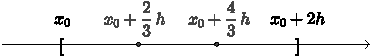
\includegraphics[width=3in]{figures/calculus-rudiments22}
\par\end{center}
\item [{\ref{exc:rudiments-30}:}] Ruas kiri hampiran, $f''\left(x_{0}+\frac{1}{2}h\right)$,
memberikan titik evaluasi untuk turunan, $x_{0}+\frac{1}{2}h$, sehingga
titik ini harus berada pada stensil dan ditandai dengan lingkaran
kosong. Ruas kanan hampiran 
\[
\frac{2f(x_{0})-8f(x_{0}+h)+8f(x_{0}+\frac{3}{2}h)-2f(x_{0}+2h)}{h^{2}}
\]
 memberikan letak simpul. Simpul-simpulnya adalah $x_{0}$, $x_{0}+h$,
$x_{0}+\frac{3}{2}h$, dan $x_{0}+2h$ dan harus ditandai dengan titik
penuh pada stensil. Dengan demikian, stensilnya adalah
\begin{center}
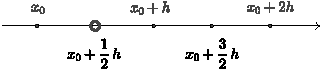
\includegraphics[width=3in]{figures/calculus-rudiments23}
\par\end{center}
\item [{\ref{exc:rudiments-31}:}] Karena simpul-simpul $0,1,2,3,$ berjarak
seragam sebesar 1, masuk akal untuk membayangkan $h=1$. Selain itu,
karena titik evaluasi $1$, kebetulan merupakan salah satu simpul,
masuk akal untuk memberi label simpul tersebut sebagai $x_{0}$. Dengan
demikian, simpul 0 seharusnya diberi label $x_{0}-h$ karena $0=1-1h$,
simpul 3 seharusnya diberi label $x_{0}+2h$ karena $3=1+2h$, dan
demikian pula simpul 2. Penetapan ini menyarankan agar kita mencari
(atau menurunkan rumus dari) stensil yang tampak seperti
\begin{center}
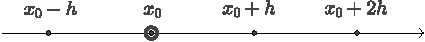
\includegraphics[width=3in]{figures/calculus-rudiments24}
\par\end{center}

Namun, pilihan $x_{0}$ dan $h$ cukup arbitrer. Kita juga dapat mencari
(atau menurunkan rumus dari) stensil yang simpul paling kirinya diberi
label $x_{0}$, seperti pada
\begin{center}
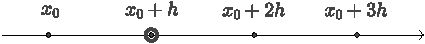
\includegraphics[width=3in]{figures/calculus-rudiments25}
\par\end{center}

Yang tidak berubah adalah bahwa kita memiliki 4 titik (simpul) berjarak
seragam dengan titik kedua dari kiri dilingkari. Posisi relatif simpul
dan titik evaluasi (geometri) adalah satu-satunya hal yang penting!
Label bersifat sekunder dan hanya penting untuk tujuan penurunan atau
penerapan rumus tertentu. Rumus yang didasarkan pada salah satu dari
kedua stensil ini, maupun berbagai stensil lain, dapat diterima sepenuhnya.
\item [{\ref{exc:rudiments-32}:}] Karena simpul-simpul $0,1.5,3,$ berjarak
seragam sebesar $1.5$, masuk akal untuk membayangkan $h=1.5$. Selain
itu, karena titik evaluasi $1$, kebetulan berada di antara simpul
paling kiri dan simpul tengah, masuk akal untuk memberi label salah
satunya sebagai $x_{0}$. Misalkan $1.5$ akan diberi label $x_{0}$.
Dengan demikian, simpul 0 seharusnya diberi label $x_{0}-h$ karena
$0=1.5-1h$ dan simpul 3 seharusnya diberi label $x_{0}+h$ karena
$3=1.5+1h$. Titik evaluasi, $1$, kemudian akan diberi label $x_{0}-\frac{1}{3}h$
karena $1=1.5-\frac{1}{3}h$. Penetapan ini menyarankan agar kita
mencari (atau menurunkan rumus dari) stensil yang tampak seperti
\begin{center}
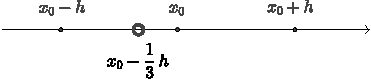
\includegraphics[width=3in]{figures/calculus-rudiments26}
\par\end{center}

Namun, pilihan $x_{0}$ dan $h$ cukup arbitrer. Kita juga dapat mencari
(atau menurunkan rumus dari) stensil yang simpul paling kirinya diberi
label $x_{0}$, seperti pada
\begin{center}
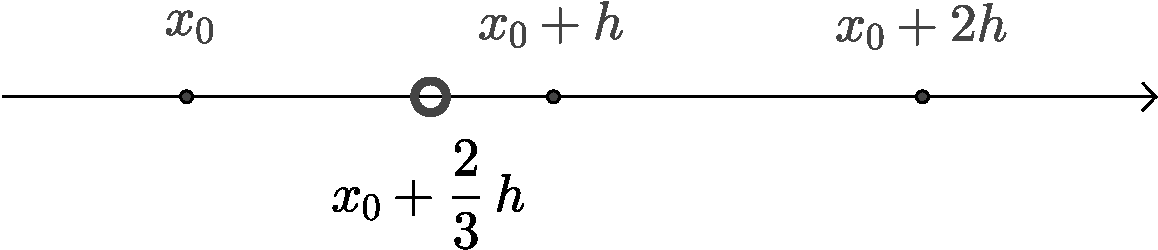
\includegraphics[width=3in]{figures/calculus-rudiments27}
\par\end{center}

Yang tidak berubah adalah bahwa kita memiliki 3 titik (simpul) berjarak
seragam dengan lingkaran (titik evaluasi) berada pada dua pertiga
jarak dari simpul paling kiri menuju simpul di sebelahnya. Posisi
relatif simpul dan titik evaluasi (geometri) adalah satu-satunya hal
yang penting! Label bersifat sekunder dan hanya penting untuk tujuan
penurunan atau penerapan rumus tertentu. Rumus yang didasarkan pada
salah satu dari kedua stensil ini, maupun berbagai stensil lain, dapat
diterima sepenuhnya.
\item [{\ref{exc:rudiments-33}:}] Karena interval integrasinya adalah
$[1,5]$, dengan lebar 4, masuk akal untuk membayangkan $h=1$, sehingga
panjang intervalnya menjadi $4h$. Dengan memberi titik ujung kiri
integrasi label $x_{0}$, simpul $1.5$ seharusnya diberi label $x_{0}+\frac{1}{2}h$
karena $1.5=1+\frac{1}{2}h$, simpul $2.5$ seharusnya diberi label
$x_{0}+\frac{3}{2}h$ karena $2.5=1+\frac{3}{2}h$, dan seterusnya.
Penetapan ini menyarankan agar kita mencari (atau menurunkan rumus
dari) stensil yang tampak seperti
\begin{center}
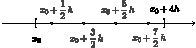
\includegraphics[width=3in]{figures/calculus-rudiments28}
\par\end{center}

Namun, pilihan $x_{0}$ dan $h$ cukup arbitrer. Umumnya kita akan
tetap menggunakan $x_{0}$ untuk titik ujung kiri interval integrasi,
tetapi $h$ dapat bervariasi. Sebagai contoh, kita juga dapat mencari
(atau menurunkan rumus dari) stensil dengan $h=\frac{1}{2}$, seperti
pada
\begin{center}
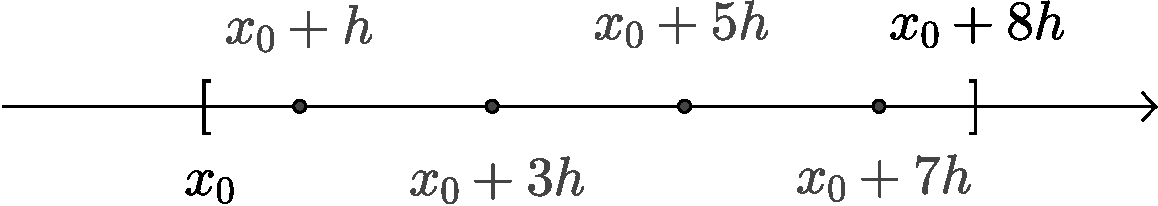
\includegraphics[width=3in]{figures/calculus-rudiments29}
\par\end{center}

Yang tidak berubah adalah bahwa kita memiliki 4 titik (simpul) berjarak
seragam di antara kedua titik ujung; titik pertama dan terakhir masing-masing
berjarak setengah jarak simpul terdekat dari titik ujung terdekat.
Posisi relatif simpul dan titik ujung (geometri) adalah satu-satunya
hal yang penting! Label bersifat sekunder dan hanya penting untuk
tujuan penurunan atau penerapan rumus tertentu. Rumus yang didasarkan
pada salah satu dari kedua stensil ini, maupun berbagai stensil lain,
dapat diterima sepenuhnya.
\item [{\ref{exc:rudiments-34}:}] Karena interval integrasinya adalah
$[1,5]$, dengan lebar 4, masuk akal untuk membayangkan $h=1$, sehingga
panjang intervalnya menjadi $4h$. Dengan memberi titik ujung kiri
integrasi label $x_{0}$, simpul $1.2$ seharusnya diberi label $x_{0}+\frac{1}{5}h$
karena $1.2=1+\frac{1}{5}h$, simpul $2.4$ seharusnya diberi label
$x_{0}+\frac{7}{5}h$ karena $2.4=1+\frac{7}{5}h$, dan seterusnya.
Penetapan ini menyarankan agar kita mencari (atau menurunkan rumus
dari) stensil yang tampak seperti
\begin{center}
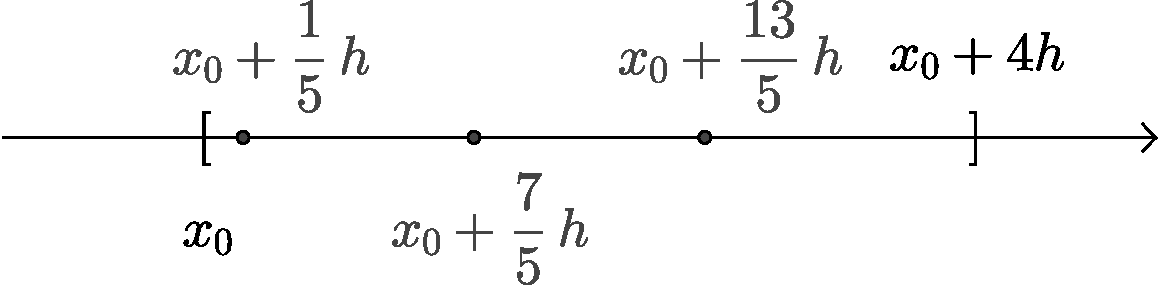
\includegraphics[width=3in]{figures/calculus-rudiments30}
\par\end{center}

Namun, pilihan $x_{0}$ dan $h$ cukup arbitrer. Umumnya kita akan
tetap menggunakan $x_{0}$ untuk titik ujung kiri interval integrasi,
tetapi $h$ dapat bervariasi. Sebagai contoh, kita juga dapat mencari
(atau menurunkan rumus dari) stensil dengan $h=\frac{1}{5}$, seperti
pada
\begin{center}
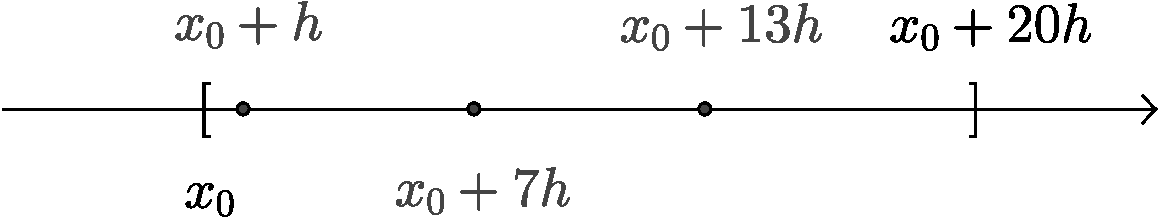
\includegraphics[width=3in]{figures/calculus-rudiments31}
\par\end{center}

Yang tidak berubah adalah bahwa kita memiliki 3 titik (simpul) berjarak
seragam di antara kedua titik ujung; titik paling kiri berjarak seperlima
jarak simpul terdekat dari titik ujung terdekat, sedangkan titik paling
kanan berjarak tujuh perlima jarak simpul terdekat dari titik ujung
terdekat. Posisi relatif simpul dan titik ujung (geometri) adalah
satu-satunya hal yang penting! Label bersifat sekunder dan hanya penting
untuk tujuan penurunan atau penerapan rumus tertentu. Rumus yang didasarkan
pada salah satu dari kedua stensil ini, maupun berbagai stensil lain,
dapat diterima sepenuhnya.
\item [{\ref{exc:rudiments}:}] (a) ${\displaystyle L_{1}(x)=\frac{x-x_{1}}{x_{0}-x_{1}}f(x_{0})+\frac{x-x_{0}}{x_{1}-x_{0}}f(x_{1})}$
(b) ${\displaystyle L_{1}'(x)=\frac{f(x_{0})}{x_{0}-x_{1}}+\frac{f(x_{1})}{x_{1}-x_{0}}=\frac{f(x_{1})-f(x_{0})}{x_{1}-x_{0}}}$
(c) $L'(x_{0}+\frac{h}{2})=\frac{f(x_{0}+h)-f(x_{0})}{x_{0}+h-x_{0}}=\frac{f(x_{0}+h)-f(x_{0})}{h}$
sehingga
\[
f'\left(x_{0}+\frac{h}{2}\right)\approx\frac{f(x_{0}+h)-f(x_{0})}{h}.
\]
\item [{\ref{exc:rudiments-6}:}] (a) Bentuk Newton dari polinom interpolasi
diperoleh dari tabel beda terbagi, baik untuk satu nilai maupun rumus
bagi kasus umum. Tabel beda terbagi untuk kasus ini adalah

\begin{center}
\begin{tabular}{c|ccc}
$x_{0}$ & $f(x_{0})$ & $\frac{f(x_{0}+h)-f(x_{0})}{h}$ & $\frac{f(x_{0}+2h)-2f(x_{0}+h)+f(x_{0})}{2h^{2}}$\tabularnewline
$x_{0}+h$ & $f(x_{0}+h)$ & $\frac{f(x_{0}+2h)-f(x_{0}+h)}{h}$ & \tabularnewline
$x_{0}+2h$ & $f(x_{0}+2h)$ &  & \tabularnewline
\end{tabular}
\begin{eqnarray*}
f_{0,1} & = & \frac{f(x_{0}+h)-f(x_{0})}{(x_{0}+h)-x_{0}}=\frac{f(x_{0}+h)-f(x_{0})}{h}\\
f_{1,1} & = & \frac{f(x_{0}+2h)-f(x_{0}+h)}{(x_{0}+2h)-(x_{0}+h)}=\frac{f(x_{0}+2h)-f(x_{0}+h)}{h}\\
f_{0,2} & = & \frac{f_{1,1}-f_{0,1}}{(x_{0}+2h)-x_{0}}=\frac{\frac{f(x_{0}+2h)-f(x_{0}+h)}{h}-\frac{f(x_{0}+h)-f(x_{0})}{h}}{2h}\\
 & = & \frac{f(x_{0}+2h)-2f(x_{0}+h)+f(x_{0})}{2h^{2}}
\end{eqnarray*}
\par\end{center}

\noindent\begin{flushleft}
Oleh karena itu, salah satu kemungkinan bentuk Newton adalah
\[
N_{2}(x)=f(x_{0})+\frac{f(x_{0}+h)-f(x_{0})}{h}(x-x_{0})+\frac{f(x_{0}+2h)-2f(x_{0}+h)+f(x_{0})}{2h^{2}}(x-x_{0})(x-(x_{0}+h)).
\]
Dengan melakukan substitusi $x_{0}+\theta h$ untuk $x$,
\[
N_{2}(x_{0}+\theta h)=f(x_{0})+\left[f(x_{0}+h)-f(x_{0})\right]\theta+\left[\frac{f(x_{0}+2h)-2f(x_{0}+h)+f(x_{0})}{2}\right](\theta)(\theta-1).
\]
(b) $\frac{dx}{d\theta}=h$ dan $\frac{d}{d\theta}N_{2}(x(\theta))=\frac{d}{dx}N_{2}(x)\cdot\frac{dx}{d\theta}$
sehingga ${\displaystyle \frac{d}{dx}N_{2}(x)=\frac{d}{d\theta}N_{2}(x(\theta))\div\frac{dx}{d\theta}=\frac{\frac{d}{d\theta}N_{2}(x(\theta))}{h}}$.
Demikian pula, kita memperoleh ${\displaystyle \frac{d^{2}}{dx^{2}}N_{2}(x)=\frac{\frac{d^{2}}{d\theta^{2}}N_{2}(x(\theta))}{h^{2}}}$:
\begin{eqnarray*}
\frac{d}{dx}N_{2}(x) & = & \frac{\left[f(x_{0}+h)-f(x_{0})\right]+\frac{f(x_{0}+2h)-2f(x_{0}+h)+f(x_{0})}{2}(2\theta-1)}{h}\\
\frac{d^{2}}{dx^{2}}N_{2}(x) & = & \frac{\frac{f(x_{0}+2h)-2f(x_{0}+h)+f(x_{0})}{2}(2)}{h\cdot h}\\
 & = & \frac{f(x_{0}+2h)-2f(x_{0}+h)+f(x_{0})}{h^{2}}.
\end{eqnarray*}
(c) $N_{2}''(x_{0}+\frac{1}{2}h)=\frac{f(x_{0}+2h)-2f(x_{0}+h)+f(x_{0})}{h^{2}}$
sehingga
\[
f''\left(x_{0}+\frac{1}{2}h\right)\approx\frac{f(x_{0}+2h)-2f(x_{0}+h)+f(x_{0})}{h^{2}}.
\]
\par\end{flushleft}
\item [{\ref{exc:rudiments-8}:}] Untuk menggunakan rumus ini, kita memerlukan
$x_{0}-h=10$ dan $x_{0}+6h=17$, suatu sistem dua persamaan dengan
dua variabel tak diketahui yang solusinya adalah $x_{0}=11$ dan $h=1$.
Dengan memasukkan nilai-nilai ini ke rumus \ref{eq:integral7dumb}:
\begin{eqnarray*}
\int_{10}^{17}\frac{1}{x-5}dx & \approx & \frac{1}{8640}\left[5257f(17)-5880f(16)+59829f(15)\right.\\
 &  & \quad\left.-81536f(14)+102459f(13)-50568f(12)+30919f(11)\right]\\
 & = & \frac{1}{8640}\left[5257\cdot\frac{1}{12}-5880\cdot\frac{1}{11}+59829\cdot\frac{1}{10}\right.\\
 &  & \quad\left.-81536\cdot\frac{1}{9}+102459\cdot\frac{1}{8}-50568\cdot\frac{1}{7}+30919\cdot\frac{1}{6}\right]\\
 & \approx & 0.8753962951271979.
\end{eqnarray*}
\item [{\ref{exc:rudiments-11}c:}] (i) $\int_{10}^{17}\frac{1}{x-5}dx=\left.\ln|x-5|\right|_{10}^{17}=\ln(12)-\ln(5)=\ln\frac{12}{5}\approx0.8754687373539001$
(ii) Galat absolut adalah nilai mutlak selisih antara hampiran dan
nilai eksak: $|\ln\frac{12}{5}-0.8753962951271979|\approx7.24(10)^{-5}$.
\item [{\ref{exc:rudiments-15}:}] Untuk menghampiri suatu besaran yang
berkaitan dengan fungsi nonpolinomial, kita cukup mengevaluasi besaran
yang bersesuaian untuk polinom interpolasi. Ini berarti bahwa dalam
kasus ini, $f'(2)\approx p'(2)$. Namun, $p'(x)=12x^{3}-4x+1$ sehingga
$f'(2)\approx12\cdot2^{3}-4\cdot2+1=89$.
\item [{\ref{exc:rudiments-19}:}] Untuk menghampiri suatu besaran yang
berkaitan dengan fungsi nonpolinomial, kita cukup mengevaluasi besaran
yang bersesuaian untuk polinom interpolasi. Ini berarti bahwa dalam
kasus ini, $\int_{0}^{1}g(x)dx\approx\int_{0}^{1}q(x)dx$:
\begin{eqnarray*}
\int_{0}^{1}g(x)dx & \approx & \int_{0}^{1}(-7x^{4}+3x^{2}-x+4)dx\\
 & = & \left[-\frac{7}{5}x^{5}+x^{3}-\frac{1}{2}x^{2}+4x\right]_{0}^{1}\\
 & = & -\frac{7}{5}+1-\frac{1}{2}+4\\
 & = & \frac{31}{10}=3.1
\end{eqnarray*}
\item [{\ref{exc:rudiments-21}:}] Untuk menggunakan rumus ini, kita hanya
perlu menyubstitusikan nilai yang tepat untuk $\theta$ dan $\theta_{i}$.
$\theta$ haruslah $0$ karena titik evaluasinya berada di $x_{0}$
(yang sama dengan $x_{0}+0h$). Tidak menjadi soal titik stensil mana
yang memberikan $\theta_{i}$ yang mana, tetapi $\theta_{i}$ berasal
dari kenyataan bahwa simpul-simpulnya adalah $x_{0}-h$, $x_{0}+2h$,
dan $x_{0}+3h$. Dengan demikian, kita memperoleh $-1,2$, dan $3$
untuk $\theta_{i}$. Dengan menetapkan $\theta_{0}=-1$, $\theta_{1}=2$,
dan $\theta_{2}=3$: 
\begin{eqnarray*}
f'(x_{0}) & \approx & P_{2}'(x)\\
 & = & \frac{(0-2)+(0-3)}{h(-1-2)(-1-3)}f(x_{0}-h)\\
 &  & +\frac{(0-(-1))+(0-3)}{h(2-(-1))(2-3)}f(x_{0}+2h)\\
 &  & +\frac{(0-(-1))+(0-2)}{h(3-(-1))(3-2)}f(x_{0}+3h)\\
 & = & -\frac{5}{12h}f(x_{0}-h)+\frac{2}{3h}f(x_{0}+2h)+\frac{-1}{4h}f(x_{0}+3h)\\
 & = & \frac{-5f(x_{0}-h)+8f(x_{0}+2h)-3f(x_{0}+3h)}{12h}.
\end{eqnarray*}
\item [{\ref{exc:rudiments-26}:}] Integral pada stensil ini membentang
dari $x_{0}$ hingga $x_{0}+2h$ sehingga $\theta_{0}=0$ dan $\theta_{1}=2$.
Simpul-simpulnya adalah $x_{0}+\frac{1}{3}h$ dan $x_{0}+\frac{4}{3}h$
sehingga $\theta_{2}$ dan $\theta_{3}$ adalah $\frac{1}{3}$ dan
$\frac{4}{3}$. Tidak menjadi soal yang mana bersesuaian dengan yang
mana. Dengan menetapkan $\theta_{2}=\frac{1}{3}$ dan $\theta_{3}=\frac{4}{3}$,
rumus dari soal \ref{exc:rudiments-24} menjadi $-\frac{h}{2}\cdot\frac{2-0}{\frac{4}{3}-\frac{1}{3}}\left((2\cdot\frac{1}{3}-2-0)f(x_{0}+\frac{4}{3}h)-(2\cdot\frac{4}{3}-2-0)f(x_{0}+\frac{1}{3}h)\right)$,
yang disederhanakan menjadi
\[
\int_{x_{0}}^{x_{0}+2h}f(x)dx\approx\frac{2h}{3}\left[f\left(x_{0}+\frac{1}{3}h\right)+2f\left(x_{0}+\frac{4}{3}h\right)\right]
\]
\end{description}

\section*{Bagian \ref{sec:UndeterminedCoefficients}}
\begin{description}
\item [{\ref{exc:undetermined}d:}] Kita hendak mencari koefisien tak tentu
$a_{i}$ pada rumus \ref{eq:derivApprox}. Kita menyelesaikan sistem
\ref{eq:systemGenericDerivative} untuk melakukannya. Stensil pada
soal ini memiliki 2 simpul, $x_{0}$ dan $x_{0}+h$, serta titik evaluasi
$x_{0}+\frac{3}{4}h$, sehingga dalam sistem \ref{eq:systemGenericDerivative}
kita memiliki $n=1$, $\theta_{0}=0$ dan $\theta_{1}=1$, serta $\theta=\frac{3}{4}$.
Karena kita sedang menurunkan rumus turunan pertama, kita juga memiliki
$k=1$. Oleh karena itu, sistem yang perlu kita selesaikan adalah
\begin{eqnarray*}
p_{0}'\left(x_{0}+\frac{3}{4}h\right) & = & a_{0}p_{0}(x_{0})+a_{1}p_{0}(x_{0}+h)\\
p_{1}'\left(x_{0}+\frac{3}{4}h\right) & = & a_{0}p_{1}(x_{0})+a_{1}p_{1}(x_{0}+h).
\end{eqnarray*}
Sekarang, $p_{0}(x)=1$ sehingga $p_{0}'(x_{0}+\frac{3}{4}h)=0;$
dan $p_{1}(x)=x-x_{0}$ sehingga $p_{1}'(x_{0}+\frac{3}{4}h)=1$.
Dengan menyubstitusikan informasi ini ke dalam sistem,
\begin{eqnarray*}
0 & = & a_{0}+a_{1}\\
1 & = & a_{1}h.
\end{eqnarray*}
Dari persamaan kedua, $a_{1}=\frac{1}{h}$. Dengan menyubstitusikannya
ke persamaan pertama, $0=a_{0}+\frac{1}{h}$ sehingga $a_{0}=-\frac{1}{h}$.
Hampiran kita, yaitu rumus \ref{eq:derivApprox}, menjadi
\begin{eqnarray*}
f'\left(x_{0}+\frac{3}{4}h\right) & \approx & -\frac{1}{h}f(x_{0})+\frac{1}{h}f(x_{0}+h)\\
 & = & \frac{f(x_{0}+h)-f(x_{0})}{h}.
\end{eqnarray*}
Rumus itu seharusnya tampak familier!
\item [{\ref{exc:undetermined}j:}] Kita hendak mencari koefisien tak tentu
$a_{i}$ pada rumus \ref{eq:derivApprox}. Kita menyelesaikan sistem
\ref{eq:systemGenericDerivative} untuk melakukannya. Stensil pada
soal ini memiliki 4 simpul, $x_{0}$, $x_{0}+h$, $x_{0}+\frac{3}{2}h$,
dan $x_{0}+2h$ dengan titik evaluasi $x_{0}+\frac{1}{2}h$, sehingga
dalam sistem \ref{eq:systemGenericDerivative} kita memiliki $n=3$,
$\theta_{0}=0$, $\theta_{1}=1$, $\theta_{2}=\frac{3}{2}$, $\theta_{3}=2$,
dan $\theta=\frac{1}{2}$. Karena kita sedang menurunkan rumus turunan
pertama, kita juga memiliki $k=1$. Oleh karena itu, sistem yang perlu
kita selesaikan adalah 
\begin{eqnarray*}
p_{0}'\left(x_{0}+\frac{1}{2}h\right) & = & a_{0}p_{0}(x_{0})+a_{1}p_{0}(x_{0}+h)+a_{2}p_{0}(x_{0}+\frac{3}{2}h)+a_{3}p_{0}(x_{0}+2h)\\
p_{1}'\left(x_{0}+\frac{1}{2}h\right) & = & a_{0}p_{1}(x_{0})+a_{1}p_{1}(x_{0}+h)+a_{2}p_{1}(x_{0}+\frac{3}{2}h)+a_{3}p_{1}(x_{0}+2h)\\
p_{2}'\left(x_{0}+\frac{1}{2}h\right) & = & a_{0}p_{2}(x_{0})+a_{1}p_{2}(x_{0}+h)+a_{2}p_{2}(x_{0}+\frac{3}{2}h)+a_{3}p_{2}(x_{0}+2h)\\
p_{3}'\left(x_{0}+\frac{1}{2}h\right) & = & a_{0}p_{2}(x_{0})+a_{1}p_{2}(x_{0}+h)+a_{2}p_{2}(x_{0}+\frac{3}{2}h)+a_{3}p_{2}(x_{0}+2h)
\end{eqnarray*}
Sekarang, $p_{0}(x)=1$ sehingga $p_{0}'(x_{0}+\frac{1}{2}h)=0;$
$p_{1}(x)=x-x_{0}$ sehingga $p_{1}'(x_{0}+\frac{1}{2}h)=1$; $p_{2}(x)=(x-x_{0})^{2}$
sehingga $p_{2}'(x_{0}+\frac{1}{2}h)=h$; dan $p_{3}(x)=(x-x_{0})^{3}$
sehingga $p_{3}'(x_{0}+\frac{1}{2}h)=\frac{3}{4}h^{2}$. Dengan menyubstitusikan
informasi ini ke dalam sistem,
\begin{eqnarray*}
0 & = & a_{0}+a_{1}+a_{2}+a_{3}\\
1 & = & a_{1}h+a_{2}\cdot\frac{3}{2}h+a_{3}\cdot2h\\
h & = & a_{1}h^{2}+a_{2}\cdot\frac{9}{4}h^{2}+a_{3}\cdot4h\\
\frac{3}{4}h^{2} & = & a_{1}h^{3}+a_{2}\cdot\frac{27}{8}h^{3}+a_{3}\cdot8h.
\end{eqnarray*}
Persamaan pertama adalah satu-satunya persamaan yang memuat $a_{0}$,
sehingga kita berfokus menyelesaikan tiga persamaan terakhir, yang
dapat disederhanakan menjadi:
\begin{eqnarray*}
\frac{2}{h} & = & 2a_{1}+3a_{2}+4a_{3}\\
\frac{4}{h} & = & 4a_{1}+9a_{2}+16a_{3}\\
\frac{6}{h} & = & 8a_{1}+27a_{2}+64a_{3}.
\end{eqnarray*}
Dari persamaan pertama, $2a_{1}=\frac{2}{h}-3a_{2}-4a_{3}$ sehingga
$4a_{1}=\frac{4}{h}-6a_{2}-8a_{3}$ dan $8a_{1}=\frac{8}{h}-12a_{2}-16a_{3}$.
Dengan menyubstitusikannya masing-masing ke persamaan kedua dan ketiga,
\begin{eqnarray*}
\frac{4}{h} & = & \frac{4}{h}-6a_{2}-8a_{3}+9a_{2}+16a_{3}\\
\frac{6}{h} & = & \frac{8}{h}-12a_{2}-16a_{3}+27a_{2}+64a_{3}
\end{eqnarray*}
yang dapat disederhanakan menjadi
\begin{eqnarray*}
0 & = & 3a_{2}+8a_{3}\\
-\frac{2}{h} & = & 15a_{2}+48a_{3}.
\end{eqnarray*}
Dari persamaan pertama, $a_{3}=-\frac{3}{8}a_{2}$. Dengan menyubstitusikannya
ke persamaan terakhir, $-\frac{2}{h}=15a_{2}+48(-\frac{3}{8}a_{2})$,
yang dapat disederhanakan menjadi $-\frac{2}{h}=-3a_{2}$ sehingga
\[
a_{2}=\frac{2}{3h}.
\]
Dengan substitusi balik, $a_{3}=-\frac{3}{8}a_{2}=-\frac{3}{8}(\frac{2}{3h})$
sehingga
\[
a_{3}=-\frac{1}{4h}.
\]
Dengan melanjutkan substitusi balik, $2a_{1}=\frac{2}{h}-3a_{2}-4a_{3}=\frac{2}{h}-3(\frac{2}{3h})-4(-\frac{1}{4h})$,
yang dapat disederhanakan menjadi $2a_{1}=\frac{1}{h}$ sehingga
\[
a_{1}=\frac{1}{2h}.
\]
Terakhir, $a_{0}=-a_{1}-a_{2}-a_{3}=-\frac{1}{2h}-\frac{2}{3h}+\frac{1}{4h}$
sehingga
\[
a_{0}=-\frac{11}{12h}.
\]
Dengan demikian, hampiran kita, yaitu rumus \ref{eq:derivApprox},
menjadi
\begin{eqnarray*}
f'\left(x_{0}+\frac{1}{2}h\right) & \approx & \frac{11}{12h}f(x_{0})+\frac{1}{2h}f(x_{0}+h)+\frac{2}{3h}f(x_{0}+\frac{3}{2}h)-\frac{1}{4h}f(x_{0}+2h)\\
 & = & \frac{-11f(x_{0})+6f(x_{0}+h)+8f(x_{0}+\frac{3}{2}h)-3f(x_{0}+2h)}{12h}.
\end{eqnarray*}
\item [{\ref{exc:undetermined-1}f:}] Kita hendak mencari koefisien tak
tentu $a_{i}$ pada rumus \ref{eq:derivApprox}. Kita menyelesaikan
sistem \ref{eq:systemGenericDerivative} untuk melakukannya. Stensil
pada soal ini memiliki 4 simpul, $x_{0}$, $x_{0}+h$, $x_{0}+\frac{3}{2}h$,
dan $x_{0}+2h$ dengan titik evaluasi $x_{0}+\frac{1}{2}h$, sehingga
dalam sistem \ref{eq:systemGenericDerivative} kita memiliki $n=3$,
$\theta_{0}=0$, $\theta_{1}=1$, $\theta_{2}=\frac{3}{2}$, $\theta_{3}=2$,
dan $\theta=\frac{1}{2}$. Karena kita sedang menurunkan rumus turunan
pertama, kita juga memiliki $k=1$. Oleh karena itu, sistem yang perlu
kita selesaikan adalah 
\begin{eqnarray*}
p_{0}''\left(x_{0}+\frac{1}{2}h\right) & = & a_{0}p_{0}(x_{0})+a_{1}p_{0}(x_{0}+h)+a_{2}p_{0}(x_{0}+\frac{3}{2}h)+a_{3}p_{0}(x_{0}+2h)\\
p_{1}''\left(x_{0}+\frac{1}{2}h\right) & = & a_{0}p_{1}(x_{0})+a_{1}p_{1}(x_{0}+h)+a_{2}p_{1}(x_{0}+\frac{3}{2}h)+a_{3}p_{1}(x_{0}+2h)\\
p_{2}''\left(x_{0}+\frac{1}{2}h\right) & = & a_{0}p_{2}(x_{0})+a_{1}p_{2}(x_{0}+h)+a_{2}p_{2}(x_{0}+\frac{3}{2}h)+a_{3}p_{2}(x_{0}+2h)\\
p_{3}''\left(x_{0}+\frac{1}{2}h\right) & = & a_{0}p_{2}(x_{0})+a_{1}p_{2}(x_{0}+h)+a_{2}p_{2}(x_{0}+\frac{3}{2}h)+a_{3}p_{2}(x_{0}+2h)
\end{eqnarray*}
Sekarang, $p_{0}(x)=1$ sehingga $p_{0}''(x_{0}+\frac{1}{2}h)=0;$
$p_{1}(x)=x-x_{0}$ sehingga $p_{1}''(x_{0}+\frac{1}{2}h)=0$; $p_{2}(x)=(x-x_{0})^{2}$
sehingga $p_{2}''(x_{0}+\frac{1}{2}h)=2$; dan $p_{3}(x)=(x-x_{0})^{3}$
sehingga $p_{3}''(x_{0}+\frac{1}{2}h)=3h$. Dengan menyubstitusikan
informasi ini ke dalam sistem,
\begin{eqnarray*}
0 & = & a_{0}+a_{1}+a_{2}+a_{3}\\
0 & = & a_{1}h+a_{2}\cdot\frac{3}{2}h+a_{3}\cdot2h\\
2 & = & a_{1}h^{2}+a_{2}\cdot\frac{9}{4}h^{2}+a_{3}\cdot4h\\
3h & = & a_{1}h^{3}+a_{2}\cdot\frac{27}{8}h^{3}+a_{3}\cdot8h.
\end{eqnarray*}
Persamaan pertama adalah satu-satunya persamaan yang memuat $a_{0}$,
sehingga kita berfokus menyelesaikan tiga persamaan terakhir, yang
dapat disederhanakan menjadi:
\begin{eqnarray*}
0 & = & 2a_{1}+3a_{2}+4a_{3}\\
\frac{8}{h^{2}} & = & 4a_{1}+9a_{2}+16a_{3}\\
\frac{24}{h^{2}} & = & 8a_{1}+27a_{2}+64a_{3}.
\end{eqnarray*}
Dari persamaan pertama, $2a_{1}=-3a_{2}-4a_{3}$ sehingga $4a_{1}=-6a_{2}-8a_{3}$
dan $8a_{1}=-12a_{2}-16a_{3}$. Dengan menyubstitusikannya masing-masing
ke persamaan kedua dan ketiga,
\begin{eqnarray*}
\frac{8}{h^{2}} & = & -6a_{2}-8a_{3}+9a_{2}+16a_{3}\\
\frac{24}{h^{2}} & = & -12a_{2}-16a_{3}+27a_{2}+64a_{3}
\end{eqnarray*}
yang dapat disederhanakan menjadi
\begin{eqnarray*}
\frac{8}{h^{2}} & = & 3a_{2}+8a_{3}\\
\frac{24}{h^{2}} & = & 15a_{2}+48a_{3}.
\end{eqnarray*}
Lima kali persamaan pertama dikurangi persamaan kedua menghasilkan
$\frac{16}{h^{2}}=-8a_{3}$ sehingga 
\[
a_{3}=-\frac{2}{h^{2}}.
\]
Dengan substitusi balik, $\frac{8}{h^{2}}=3a_{2}+8a_{3}=3a_{2}+8(-\frac{2}{h^{2}})$
sehingga
\[
a_{2}=\frac{8}{h^{2}}.
\]
Dengan melanjutkan substitusi balik, $2a_{1}=-3a_{2}-4a_{3}=-3(\frac{8}{h^{2}})-4(-\frac{2}{h^{2}})$,
yang dapat disederhanakan menjadi $2a_{1}=-\frac{16}{h^{2}}$ sehingga
\[
a_{1}=-\frac{8}{h^{2}}.
\]
Terakhir, $a_{0}=-a_{1}-a_{2}-a_{3}=\frac{8}{h^{2}}-\frac{8}{h^{2}}+\frac{2}{h^{2}}$
sehingga
\[
a_{0}=\frac{2}{h^{2}}.
\]
Dengan demikian, hampiran kita, yaitu rumus \ref{eq:derivApprox},
menjadi
\begin{eqnarray*}
f''\left(x_{0}+\frac{1}{2}h\right) & \approx & \frac{2}{h^{2}}f(x_{0})-\frac{8}{h^{2}}f(x_{0}+h)+\frac{8}{h^{2}}f(x_{0}+\frac{3}{2}h)-\frac{2}{h^{2}}f(x_{0}+2h)\\
 & = & \frac{2f(x_{0})-8f(x_{0}+h)+8f(x_{0}+\frac{3}{2}h)-2f(x_{0}+2h)}{h^{2}}.
\end{eqnarray*}
\item [{\ref{exc:undetermined-2}b:}] Kita hendak mencari koefisien tak
tentu $a_{i}$ pada rumus \ref{eq:integralApprox}. Kita menyelesaikan
sistem \ref{eq:systemGenericIntegral} untuk melakukannya. Stensil
pada soal ini memiliki 1 simpul, $x_{0}+\frac{2}{3}h$ serta titik-titik
ujung integrasi $x_{0}$ dan $x_{0}+2h$, sehingga dalam sistem \ref{eq:systemGenericIntegral}
kita memiliki $n=0$, $a=x_{0}$ dan $b=x_{0}+2h$. Oleh karena itu,
``sistem'' yang perlu kita selesaikan adalah 
\[
\int_{x_{0}}^{x_{0}+2h}p_{0}(x)dx=a_{0}p_{0}(x_{0}).
\]
Sekarang, $p_{0}(x)=1$ sehingga $\int_{x_{0}}^{x_{0}+2h}p_{0}(x)dx=\int_{x_{0}}^{x_{0}+2h}dx=2h$.
Dengan menyubstitusikan informasi ini ke dalam sistem,
\[
2h=a_{0}.
\]
Hampiran kita, yaitu rumus \ref{eq:integralApprox}, menjadi
\[
\int_{x_{0}}^{x_{0}+2h}f(x)dx\approx2hf\left(x_{0}+\frac{2}{3}h\right).
\]
\item [{\ref{exc:undetermined-2}l:}] Kita hendak mencari koefisien tak
tentu $a_{i}$ pada rumus \ref{eq:integralApprox}. Kita menyelesaikan
sistem \ref{eq:systemGenericIntegral} untuk melakukannya. Stensil
pada soal ini memiliki 3 simpul, $x_{0}$, $x_{0}+h$, dan $x_{0}+2h$
dengan titik-titik ujung integrasi $x_{0}$ dan $x_{0}+2h$, sehingga
dalam sistem \ref{eq:systemGenericIntegral} kita memiliki $n=2$,
$a=x_{0}$ dan $b=x_{0}+2h$. Oleh karena itu, sistem yang perlu kita
selesaikan adalah 
\begin{eqnarray*}
\int_{x_{0}}^{x_{0}+2h}p_{0}(x)dx & = & a_{0}p_{0}(x_{0})+a_{1}p_{0}(x_{0}+h)+a_{2}p_{0}(x_{0}+2h)\\
\int_{x_{0}}^{x_{0}+2h}p_{1}(x)dx & = & a_{0}p_{1}(x_{0})+a_{1}p_{1}(x_{0}+h)+a_{2}p_{1}(x_{0}+2h)\\
\int_{x_{0}}^{x_{0}+2h}p_{2}(x)dx & = & a_{0}p_{2}(x_{0})+a_{1}p_{2}(x_{0}+h)+a_{2}p_{2}(x_{0}+2h)
\end{eqnarray*}
Sekarang, $p_{0}(x)=1$ sehingga $\int_{x_{0}}^{x_{0}+2h}p_{0}(x)dx=\int_{x_{0}}^{x_{0}+2h}dx=2h$;
$p_{1}(x)=x-x_{0}$ sehingga $\int_{x_{0}}^{x_{0}+2h}p_{1}(x)dx=\int_{x_{0}}^{x_{0}+2h}(x-x_{0})dx=\left.\frac{1}{2}(x-x_{0})^{2}\right|_{x_{0}}^{x_{0}+2h}=2h^{2}$;
dan $p_{2}(x)=(x-x_{0})^{2}$ sehingga $\int_{x_{0}}^{x_{0}+2h}p_{2}(x)dx=\int_{x_{0}}^{x_{0}+2h}(x-x_{0})^{2}dx=\left.\frac{1}{3}(x-x_{0})^{3}\right|_{x_{0}}^{x_{0}+2h}=\frac{8}{3}h^{3}$.
Dengan menyubstitusikan informasi ini ke dalam sistem,
\begin{eqnarray*}
2h & = & a_{0}+a_{1}+a_{2}\\
2h^{2} & = & a_{1}h+a_{2}(2h)\\
\frac{8}{3}h^{3} & = & a_{1}h^{2}+a_{2}(4h^{2}).
\end{eqnarray*}
Persamaan pertama adalah satu-satunya persamaan yang memuat $a_{0}$,
sehingga kita berfokus pada dua persamaan terakhir, yang dapat disederhanakan
menjadi:
\begin{eqnarray*}
2h & = & a_{1}+2a_{2}\\
\frac{8}{3}h & = & a_{1}+4a_{2}.
\end{eqnarray*}
Dari persamaan pertama, $a_{1}=2h-2a_{2}$. Dengan menyubstitusikannya
ke persamaan kedua, $\frac{8}{3}h=2h-2a_{2}+4a_{2}$, yang dapat disederhanakan
menjadi $\frac{2}{3}h=2a_{2}$, sehingga
\[
a_{2}=\frac{1}{3}h.
\]
Dengan substitusi balik, $a_{1}=2h-2a_{2}=2h-2(\frac{1}{3}h)$ sehingga
\[
a_{1}=\frac{4}{3}h.
\]
Terakhir, $a_{0}=2h-a_{1}-a_{2}=2h-\frac{4}{3}h-\frac{1}{3}h$ sehingga
\[
a_{0}=\frac{1}{3}h.
\]
Dengan demikian, hampiran kita, yaitu rumus \ref{eq:integralApprox},
menjadi
\begin{eqnarray*}
\int_{x_{0}}^{x_{0}+2h}f(x)dx & \approx & \frac{1}{3}hf(x_{0})+\frac{4}{3}hf(x_{0}+h)+\frac{1}{3}f(x_{0}+2h)\\
 & = & \frac{h}{3}\left[f(x_{0})+4f(x_{0}+h)+f(x_{0}+2h)\right].
\end{eqnarray*}
Anda mungkin mengenali rumus ini sebagai Aturan Simpson!
\end{description}

\section*{Bagian \ref{sec:calculusErrorAnalysis}}
\begin{description}
\item [{\ref{exc:calculusErrors-5}:}] Aturan Simpson untuk hampiran integral
adalah ${\displaystyle \int_{x_{0}}^{x_{0}+2h}f(x)dx=\frac{h}{3}\left[f(x_{0})+4f(x_{0}+h)+f(x_{0}+2h)\right]}$.
Untuk menerapkannya pada integral ${\displaystyle \int_{-0.5}^{0}x\ln(x+1)dx}$
kita perlu menentukan $f$, $x_{0}$, dan $h$. Dalam rumus tersebut,
$x_{0}$ adalah batas bawah integrasi, sehingga pada soal ini kita
memiliki $x_{0}=-0.5$. Dalam rumus tersebut, panjang interval integrasi
adalah $2h$, sehingga pada soal ini kita memiliki $2h=0.5$, atau
$h=0.25$. Dalam rumus tersebut, $f$ adalah integran, sehingga kita
memiliki $f(x)=x\ln(x+1)$. Setelah parameternya ditentukan, kita
memasukkannya ke ruas kanan Aturan Simpson dan memperoleh taksiran:
\begin{eqnarray*}
{\displaystyle \int_{-0.5}^{0}x\ln(x+1)dx} & \approx & \frac{.25}{3}\left[-0.5\ln(0.5)+4(-0.25)\ln(.75)+0\ln(1)\right]\\
 & \approx & 0.05285463856097945.
\end{eqnarray*}
\item [{\ref{exc:calculusErrors-1}a:}] Aturan Trapesium untuk hampiran
integral adalah ${\displaystyle \int_{x_{0}}^{x_{0}+h}f(x)dx=\frac{h}{2}\left[f(x_{0})+f(x_{0}+h)\right]}$.
Untuk menerapkannya pada integral ${\displaystyle \int_{-0.5}^{0}x\ln(x+1)dx}$
kita perlu menentukan $f$, $x_{0}$, dan $h$. Dalam rumus tersebut,
$x_{0}$ adalah batas bawah integrasi, sehingga pada soal ini kita
memiliki $x_{0}=-0.5$. Dalam rumus tersebut, panjang interval integrasi
adalah $h$, sehingga pada soal ini kita memiliki $h=0.5$. Dalam
rumus tersebut, $f$ adalah integran, sehingga kita memiliki $f(x)=x\ln(x+1)$.
Setelah parameternya ditentukan, kita memasukkannya ke ruas kanan
Aturan Trapesium dan memperoleh taksiran:
\begin{eqnarray*}
{\displaystyle \int_{-0.5}^{0}x\ln(x+1)dx} & \approx & \frac{.5}{2}\left[-0.5\ln(0.5)+0\ln(1)\right]\\
 & \approx & 0.08664339756999316.
\end{eqnarray*}
\item [{\ref{exc:calculusErrors-2}a:}] Aturan Titik Tengah untuk hampiran
integral adalah ${\displaystyle \int_{x_{0}}^{x_{0}+2h}f(x)dx=2hf(x_{0}+h)}$.
Untuk menerapkannya pada integral 
\[
{\displaystyle \int_{-0.5}^{0}x\ln(x+1)dx},
\]
kita perlu menentukan $f$, $x_{0}$, dan $h$. Dalam rumus tersebut,
$x_{0}$ adalah batas bawah integrasi, sehingga pada soal ini kita
memiliki $x_{0}=-0.5$. Dalam rumus tersebut, panjang interval integrasi
adalah $2h$, sehingga pada soal ini kita memiliki $2h=0.5$, atau
$h=0.25$. Dalam rumus tersebut, $f$ adalah integran, sehingga kita
memiliki $f(x)=x\ln(x+1)$. Setelah parameternya ditentukan, kita
memasukkannya ke ruas kanan Aturan Trapesium dan memperoleh taksiran:
\begin{eqnarray*}
{\displaystyle \int_{-0.5}^{0}x\ln(x+1)dx} & \approx & 2(.25)(-0.25\ln(0.75))\\
 & \approx & 0.03596025905647261.
\end{eqnarray*}
\item [{\ref{exc:calculusErrors-37}a:}] Dengan menggunakan integrasi parsial,
\begin{eqnarray*}
\int_{-0.5}^{0}x\ln(x+1)dx & = & \left.\frac{x^{2}}{2}\ln(x+1)\right|_{-0.5}^{0}-\frac{1}{2}\int_{-0.5}^{0}\frac{x^{2}}{x+1}dx\\
 & = & -\frac{(-0.5)^{2}}{2}\ln(0.5)-\frac{1}{2}\int_{-0.5}^{0}\left(x-1+\frac{1}{x+1}\right)dx\\
 & = & -.125\ln(.5)-\frac{1}{2}\left[\frac{x^{2}}{2}-x+\ln|x+1|\right]_{-0.5}^{0}\\
 & = & -.125\ln(.5)+\frac{1}{2}\left[\frac{.25}{2}+.5+\ln(.5)\right]\\
 & = & .3125+.375\ln(.5)\\
 & \approx & 0.05256980729002053
\end{eqnarray*}
sehingga galatnya adalah $|0.05285463856097945-0.05256980729002053|\approx2.8483(10)^{-4}$.
\item [{\ref{exc:calculusErrors-38}a:}] Lihat di atas untuk evaluasi eksak
integral tersebut. Galatnya diperoleh sebagai\\
$|0.08664339756999316-0.05256980729002053|\approx0.034073$.
\item [{\ref{exc:calculusErrors-39}a:}] Lihat di atas untuk evaluasi eksak
integral tersebut. Galatnya diperoleh sebagai\\
$|0.03596025905647261-0.05256980729002053|\approx0.016609$.
\item [{\ref{exc:calculusErrors-36}:}] $-\frac{h^{2}}{6}f'''(\xi_{h})$
adalah suku galat untuk rumus hampiran ini. Bagian lain dari persamaan
tersebut adalah hampirannya. Kita cukup memasukkan informasi yang
diberikan ke rumus hampiran: 
\begin{eqnarray*}
f'(x_{0}) & \approx & \frac{f(x_{0}+h)-f(x_{0}-h)}{2h}\\
 & = & \frac{e^{2.1}-e^{1.9}}{2(.1)}\\
 & \approx & 7.401377351441916.
\end{eqnarray*}
\item [{\ref{exc:calculusErrors-8}a:}] Suku galat, $-\frac{h^{2}}{6}f'''(\xi_{h})$,
menentukan galat. Seperti dalam Teorema Taylor, suku galat ini eksak
untuk suatu nilai $\xi_{h}$. Mencari batas galat berarti meminimumkan
atau memaksimumkan $|\frac{h^{2}}{6}f'''(\xi_{h})|$ untuk semua nilai
$\xi_{h}$ yang mungkin. Nilai-nilai $\xi_{h}$ yang mungkin adalah
semua nilai di antara simpul terkecil dan terbesar, suatu fakta yang
diperoleh dari Teorema Taylor. Untuk soal ini, $h=.1$ dan $f'''(\xi)=e^{\xi}$,
sehingga batas bawah galat adalah 
\[
\frac{.1^{2}}{6}\min_{\xi\in[1.9,2.1]}e^{\xi}
\]
dan batas atasnya adalah
\[
\frac{.1^{2}}{6}\max_{\xi\in[1.9,2.1]}e^{\xi}.
\]
Namun, $e^{\xi}$ adalah fungsi naik, sehingga nilai minimumnya pada
$[1.9,2.1]$ dicapai di $1.9$ dan nilai maksimumnya di $2.1$. Jadi,
galatnya berada di antara $\frac{.01}{6}e^{1.9}$ dan $\frac{.01}{6}e^{2.1}$,
atau sebagai hampiran titik-mengambang, $0.01114315740379878$ dan
$0.01361028318761275$. $f'(x)=e^{x}$ sehingga $f'(2)=e^{2}$ secara
eksak. Dengan demikian, galat sebenarnya adalah $|e^{2}-7.401377351441916|\approx0.01232125251126526$,
yang berada di antara kedua batas tersebut.
\item [{\ref{exc:calculusErrors-9}a:}] Rincian lengkap rumus memuat syarat
tersirat ``untuk suatu $\xi_{h}\in(x_{0}-h,x_{0}+h)$'', dengan
interval yang ditentukan oleh simpul terkecil dan terbesar. Jadi,
kita mencari nilai $\xi_{h}$ sedemikian sehingga
\[
f'(x_{0})=\frac{f(x_{0}+h)-f(x_{0}-h)}{2h}-\frac{h^{2}}{6}f'''(\xi_{h})
\]
dan $\xi_{h}\in(x_{0}-h,x_{0}+h)$. $f$, $x_{0}$, dan $h$ telah
diberikan, sehingga kita menyubstitusikannya ke persamaan ini dan
menyelesaikannya. Namun pertama-tama, perhatikan bahwa $f'(x)=e^{x}$
dan $f'''(x)=e^{x}$:
\begin{eqnarray*}
e^{2} & = & \frac{e^{2.1}-e^{1.9}}{.2}-\frac{.1^{2}}{6}e^{\xi_{h}}\\
\frac{.01}{6}e^{\xi_{h}} & = & \frac{e^{2.1}-e^{1.9}-.2e^{2}}{.2}\\
e^{\xi_{h}} & = & \frac{6}{.002}\left[e^{2.1}-e^{1.9}-.2e^{2}\right]\\
\xi_{h} & = & \ln(3000(e^{2.1}-e^{1.9}-.2e^{2}))\\
 & \approx & 2.00049999404725,
\end{eqnarray*}
dan $\xi_{h}\in(1.9,2.1)$ seperti yang dipersyaratkan.
\item [{\ref{exc:calculusErrors-10}:}] Derajat ketelitiannya adalah 4
karena suku galat memuat turunan kelima dari $f$. Turunan kelima
setiap polinom berderajat 4 atau kurang identik dengan nol, sehingga
jika $f$ adalah polinom berderajat 4 atau kurang, galat penggunaan
rumus hampiran adalah nol.
\item [{\ref{exc:calculusErrors-11}:}] \label{sol:exc:calculusErrors-11}Galat
dalam setiap rumus hampiran adalah selisih antara kedua ruas. Satu
ruas memuat besaran eksak dan ruas lainnya memuat hampirannya. Untuk
mencari galat, kita mengurangkan kedua ruas, mengembangkan setiap
kemunculan $f$ dalam deret Taylor di sekitar $x_{0}$ dan menyederhanakannya.
Suku berderajat terendah yang tersisa menentukan suku galat.

Ruas kiri hampiran ini adalah $\int_{x_{0}}^{x_{0}+h}f(x)dx$, jadi
gantikan $f(x)$ dengan $f(x_{0})+(x-x_{0})f'(x_{0})+\frac{1}{2}(x-x_{0})^{2}f''(x_{0})+\frac{1}{6}(x-x_{0})^{3}f'''(x_{0})+\cdots$:
\begin{eqnarray*}
\int_{x_{0}}^{x_{0}+h}f(x)dx & = & \int_{x_{0}}^{x_{0}+h}\left[f(x_{0})+(x-x_{0})f'(x_{0})+\frac{1}{2}(x-x_{0})^{2}f''(x_{0})+\frac{1}{6}(x-x_{0})^{3}f'''(x_{0})+\cdots\right]dx\\
 & = & \left[xf(x_{0})+\frac{1}{2}(x-x_{0})^{2}f'(x_{0})+\frac{1}{6}(x-x_{0})^{3}f''(x_{0})+\frac{1}{24}(x-x_{0})^{4}f'''(x_{0})+\cdots\right]_{x_{0}}^{x_{0}+h}\\
 & = & hf(x_{0})+\frac{1}{2}h^{2}f'(x_{0})+\frac{1}{6}h^{3}f''(x_{0})+\frac{1}{24}h^{4}f'''(x_{0})+\cdots.
\end{eqnarray*}
Ruas kanan hampiran memuat $f(x_{0}+\frac{2}{3}h)$, sehingga ekspresi
ini juga dikembangkan dalam deret Taylor:
\[
f\left(x_{0}+\frac{2}{3}h\right)=f(x_{0})+\frac{2}{3}hf'(x_{0})+\frac{2}{9}h^{2}f''(x_{0})+\frac{4}{81}h^{3}f'''(x_{0})+\cdots.
\]
Substitusikan pengembangan ini ke selisih kedua ruas lalu sederhanakan.
Galatnya adalah
\[
\begin{gathered}\left(hf(x_{0})+\frac{1}{2}h^{2}f'(x_{0})+\frac{1}{6}h^{3}f''(x_{0})+\frac{1}{24}h^{4}f'''(x_{0})+\cdots\right)\\
-\frac{h}{4}\left[3\left(f(x_{0})+\frac{2}{3}hf'(x_{0})+\frac{2}{9}h^{2}f''(x_{0})+\frac{4}{81}h^{3}f'''(x_{0})+\cdots\right)+f(x_{0})\right]\\
=\\
\left(hf(x_{0})+\frac{1}{2}h^{2}f'(x_{0})+\frac{1}{6}h^{3}f''(x_{0})+\frac{1}{24}h^{4}f'''(x_{0})+\cdots\right)\\
-\left(hf(x_{0})+\frac{1}{2}h^{2}f'(x_{0})+\frac{1}{6}h^{3}f''(x_{0})+\frac{1}{27}h^{4}f'''(x_{0})+\cdots\right)\\
=\\
\frac{1}{216}h^{4}f'''(x_{0})+\cdots.
\end{gathered}
\]
Perhitungan sebelumnya merupakan bukti informal bahwa suku galatnya
adalah $O(h^{4}f'''(\xi_{h}))$. Untuk memformalkannya, kita memenggal
deret Taylor sehingga menjadi polinomial Taylor berderajat yang sesuai,
\textit{dengan} suku galat! Suku galat dari polinomial Taylor menjadi
suku galat untuk rumus hampiran. Dimulai dari ruas kiri rumus, yaitu
nilai eksak:
\begin{eqnarray*}
\int_{x_{0}}^{x_{0}+h}f(x)dx & = & \int_{x_{0}}^{x_{0}+h}\left[f(x_{0})+(x-x_{0})f'(x_{0})+\frac{1}{2}(x-x_{0})^{2}f''(x_{0})+\frac{1}{6}(x-x_{0})^{3}f'''(\xi_{x})\right]dx\\
 & = & \left[xf(x_{0})+\frac{1}{2}(x-x_{0})^{2}f'(x_{0})+\frac{1}{6}(x-x_{0})^{3}f''(x_{0})\right]_{x_{0}}^{x_{0}+h}\\
 &  & \qquad\qquad\qquad\qquad\qquad\qquad\qquad+\int_{x_{0}}^{x_{0}+h}\frac{1}{6}(x-x_{0})^{3}f'''(\xi_{x})dx\\
 & = & hf(x_{0})+\frac{1}{2}h^{2}f'(x_{0})+\frac{1}{6}h^{3}f''(x_{0})+\int_{x_{0}}^{x_{0}+h}\frac{1}{6}(x-x_{0})^{3}f'''(\xi_{x})dx
\end{eqnarray*}
untuk suatu fungsi tak diketahui $\xi_{x}$ dari $x$. Sekarang, suku
$f(x_{0}+\frac{2}{3}h)$ dari ruas kanan rumus, yaitu nilai hampiran:
\[
f\left(x_{0}+\frac{2}{3}h\right)=f(x_{0})+\frac{2}{3}hf'(x_{0})+\frac{2}{9}h^{2}f''(x_{0})+\frac{4}{81}h^{3}f'''(\xi_{1})
\]
untuk suatu $\xi_{1}\in(x_{0},x_{0}+h)$. Dengan mengurangkan kedua
ruas, kita tahu bahwa semua suku dengan turunan berorde lebih rendah
daripada tiga akan saling meniadakan karena tidak satu pun suku tersebut
berubah sejak temuan kita. Oleh karena itu, galatnya adalah
\[
\int_{x_{0}}^{x_{0}+h}\frac{1}{6}(x-x_{0})^{3}f'''(\xi_{x})dx-\frac{h}{4}\cdot3\cdot\frac{4}{81}h^{3}f'''(\xi_{1}).
\]
Teorema Nilai Rata-Rata Berbobot\index{Teorema!Nilai Rata-Rata Berbobot}
memungkinkan kita mengganti $\int_{x_{0}}^{x_{0}+h}\frac{1}{6}(x-x_{0})^{3}f'''(\xi_{x})dx$
dengan $\frac{1}{6}f'''(c)\int_{x_{0}}^{x_{0}+h}(x-x_{0})^{3}dx=\frac{1}{24}h^{4}f'''(c)$
untuk suatu $c\in(x_{0},x_{0}+h)$. Dengan demikian, suku galat menjadi
\[
\frac{1}{24}h^{4}f'''(c)-\frac{1}{27}h^{4}f'''(\xi_{1})
\]
untuk suatu $c\in(x_{0},x_{0}+h)$ dan suatu $\xi_{1}\in(x_{0},x_{0}+h)$.
Formalitas terakhir adalah mengganti suku ini dengan notasi O-besar:
\begin{eqnarray*}
\left|\frac{1}{24}h^{4}f'''(c)-\frac{1}{27}h^{4}f'''(\xi_{1})\right| & \leq & h^{4}\left(\frac{1}{24}\left|f'''(c)\right|+\frac{1}{27}\left|f'''(\xi_{1})\right|\right)\\
 & \leq & h^{4}\left(\frac{1}{24}+\frac{1}{27}\right)\max\left\{ \left|f'''(c)\right|,\left|f'''(\xi_{1})\right|\right\} \\
 & = & Mh^{4}\left|f'''(\xi_{h})\right|
\end{eqnarray*}
untuk suatu $\xi_{h}\in(x_{0},x_{0}+h)$ dan $M=\frac{1}{24}+\frac{1}{27}=\frac{17}{216}$
(nilai $\xi_{h}$ adalah $c$ atau $\xi_{1}$). Jadi, galatnya adalah
$O(h^{4}f'''(\xi_{h}))$.
\item [{\ref{exc:calculusErrors-12}:}] Galat dalam setiap rumus hampiran
adalah selisih antara kedua ruas. Satu ruas memuat besaran eksak dan
ruas lainnya memuat hampirannya. Untuk mencari galat, kita mengurangkan
kedua ruas, mengembangkan setiap kemunculan $f$ dalam deret Taylor
di sekitar $x_{0}$ dan menyederhanakannya. Suku berderajat terendah
yang tersisa menentukan suku galat. ${\displaystyle f'(x_{0})\approx\frac{-3f(x_{0})+4f(x_{0}+\frac{h}{2})-f(x_{0}+h)}{h}}$

Ruas kiri hampiran ini adalah $f'(x_{0})$, sehingga ekspansi Taylornya
adalah ruas itu sendiri! Ruas kanan hampiran memuat $f(x_{0}+\frac{1}{2}h)$
dan $f(x_{0}+h)$, sehingga ekspresi tersebut dikembangkan dalam deret
Taylor:
\begin{eqnarray*}
f\left(x_{0}+\frac{1}{2}h\right) & = & f(x_{0})+\frac{1}{2}hf'(x_{0})+\frac{1}{8}h^{2}f''(x_{0})+\frac{1}{48}h^{3}f'''(x_{0})+\cdots\\
f\left(x_{0}+h\right) & = & f(x_{0})+hf'(x_{0})+\frac{1}{2}h^{2}f''(x_{0})+\frac{1}{6}h^{3}f'''(x_{0})+\cdots.
\end{eqnarray*}
Untuk menyederhanakan penyajian aljabar, kita mulai dengan menjumlahkan
$-3f(x_{0})+4f(x_{0}+\frac{h}{2})-f(x_{0}+h)$:

\begin{center}
\begin{tabular}{rcl}
$-3f(x_{0})$ & $=$ & $-3f(x_{0})$\tabularnewline
$4f(x_{0}+\frac{1}{2}h)$ & $=$ & $4f(x_{0})+2hf'(x_{0})+\frac{1}{2}h^{2}f''(x_{0})+\frac{1}{12}h^{3}f'''(x_{0})+\cdots$\tabularnewline
$-f(x_{0}+h)$ & $=$ & $-f(x_{0})-hf'(x_{0})-\frac{1}{2}h^{2}f''(x_{0})-\frac{1}{6}h^{3}f'''(x_{0})+\cdots$\tabularnewline
\hline 
$-3f(x_{0})+4f(x_{0}+\frac{h}{2})-f(x_{0}+h)$ & $=$ & $hf'(x_{0})-\frac{1}{12}h^{3}f'''(x_{0})+\cdots$.\tabularnewline
\end{tabular}
\par\end{center}

\noindent Selisih kedua ruas kemudian adalah
\[
f'(x_{0})-\frac{hf'(x_{0})-\frac{1}{12}h^{3}f'''(x_{0})+\cdots}{h}=\frac{1}{12}h^{2}f'''(x_{0}).
\]
Perhitungan sebelumnya merupakan bukti informal bahwa suku galatnya
adalah $O(h^{2}f'''(\xi_{h}))$. Untuk memformalkannya, kita memenggal
deret Taylor sehingga menjadi polinomial Taylor berderajat yang sesuai,
\textit{dengan} suku galat! Suku galat dari polinomial Taylor menjadi
suku galat untuk rumus hampiran. Sekali lagi, ruas kiri merupakan
ekspansi Taylor! Sekarang, suku $f(x_{0}+\frac{1}{2}h)$ dan $f(x_{0}+h)$
dari ruas kanan rumus:
\begin{eqnarray*}
f\left(x_{0}+\frac{1}{2}h\right) & = & f(x_{0})+\frac{1}{2}hf'(x_{0})+\frac{1}{8}h^{2}f''(x_{0})+\frac{1}{48}h^{3}f'''(\xi_{1})\\
f\left(x_{0}+h\right) & = & f(x_{0})+hf'(x_{0})+\frac{1}{2}h^{2}f''(x_{0})+\frac{1}{6}h^{3}f'''(\xi_{2})
\end{eqnarray*}
untuk suatu $\xi_{1},\xi_{2}\in(x_{0},x_{0}+h)$. Dengan mengurangkan
kedua ruas, kita tahu bahwa semua suku dengan turunan berorde lebih
rendah daripada tiga akan saling meniadakan karena tidak satu pun
suku tersebut berubah sejak temuan kita. Suku-suku yang tersisa, yaitu
suku yang memuat turunan ketiga, merupakan galat dan bernilai
\[
\frac{-4\cdot\frac{1}{48}h^{3}f'''(\xi_{1})+\frac{1}{6}h^{3}f'''(\xi_{2})}{h}=h^{2}\left(\frac{1}{6}f'''(\xi_{2})-\frac{1}{12}f'''(\xi_{1})\right)
\]
untuk suatu $\xi_{1},\xi_{2}\in(x_{0},x_{0}+h)$. Formalitas terakhir
adalah mengganti suku ini dengan notasi O-besar:
\begin{eqnarray*}
\left|h^{2}\left(\frac{1}{6}f'''(\xi_{2})-\frac{1}{12}f'''(\xi_{1})\right)\right| & \leq & h^{2}\left(\frac{1}{6}\left|f'''(\xi_{2})\right|+\frac{1}{12}\left|f'''(\xi_{1})\right|\right)\\
 & \leq & h^{2}\left(\frac{1}{6}+\frac{1}{12}\right)\max\left\{ \left|f'''(\xi_{2})\right|,\left|f'''(\xi_{1})\right|\right\} \\
 & = & Mh^{2}\left|f'''(\xi_{h})\right|
\end{eqnarray*}
untuk suatu $\xi_{h}\in(x_{0},x_{0}+h)$ dan $M=\frac{1}{6}+\frac{1}{12}=\frac{1}{4}$
(nilai $\xi_{h}$ adalah $\xi_{2}$ atau $\xi_{1}$). Jadi, galatnya
adalah $O(h^{2}f'''(\xi_{h}))$.
\item [{\ref{exc:calculusErrors-17}:}] Diffy Rence menggunakan rumus turunan
kedua dengan $x_{0}=3$ karena ruas kirinya adalah $f''(3.0)$. Pada
ruas kanan, kita melihat suku yang memuat $\sin(3)$ di dalamnya.
Kemungkinan ini adalah $\sin(x_{0})$ dari salah satu rumus turunan
kedua. Kita juga melihat $\sin(2.8)$ dan $\sin(3.2)$ yang tampaknya
berperan sebagai $\sin(x_{0}-h)$ dan $\sin(x_{0}+h)$ dalam rumus
hampiran yang digunakan. Dengan melihat Tabel \ref{tab:secondDerivativeFormulas}
untuk rumus yang memuat $f(x_{0}-h)$, $f(x_{0})$, dan $f(x_{0}+h)$,
kita menemukan $f''(x_{0})=\frac{f(x_{0}-h)-2f(x_{0})+f(x_{0}+h)}{h^{2}}+O(h^{2}f^{(4)}(\xi_{h}))$.
Dengan melanjutkan hipotesis bahwa kita memiliki $f(x)=\sin(x)$,
$x_{0}=3$, dan $h=.2$, kita memasukkannya ke rumus untuk memperoleh
\begin{eqnarray*}
f''(3) & \approx & \frac{\sin(2.8)-2\sin(3)+\sin(3.2)}{.2^{2}}\\
 & = & 25\left[\sin(2.8)-2\sin(3)+\sin(3.2)\right].
\end{eqnarray*}
Kita menyimpulkan bahwa $f(x)=\sin x$. 
\item [{\ref{exc:calculusErrors-13}:}] Pertama-tama, kita perlu menentukan
rumus yang digunakan. Karena ini adalah rumus turunan ketiga dengan
$x_{0}=3$ dan evaluasi $f$ pada $3,3.01,3.02,3.03,3.04$, ini adalah
rumus lima titik dengan $h=.01$. Rumus yang digunakan adalah rumus
berikut dari Tabel \ref{tab:thirdDerivativeFormulas}:
\[
f'''(x_{0})=\frac{-5f(x_{0})+18f(x_{0}+h)-24f(x_{0}+2h)+14f(x_{0}+3h)-3f(x_{0}+4h)}{2h^{3}}+O(h^{2}f^{(5)}(\xi_{h}))
\]
sehingga suku galatnya adalah $O(h^{2}f^{(5)}(\xi_{h}))$. Oleh karena
itu, galat dibatasi oleh 
\[
k(.01)^{2}\max_{x\in[3,3.04]}\left|f^{(5)}(x)\right|
\]
untuk suatu konstanta $k$ yang bergantung pada \textit{metode}, bukan
pada fungsi $f$ atau simpul yang digunakan. Sekarang,
\begin{eqnarray*}
\max_{x\in[3,3.04]}\left|f^{(5)}(x)\right| & = & \max_{x\in[3,3.04]}\left|\cos(x)\right|\\
 & = & \left|\cos(3.04)\right|.
\end{eqnarray*}
Dengan demikian, batas galatnya adalah $0.0001k\cos(3.04)$ atau $9.9485(10)^{-5}k$
untuk suatu $k$ yang bergantung pada \textit{metode}.
\item [{\ref{exc:calculusErrors-14}:}] Pertama-tama, kita perlu menentukan
rumus yang digunakan. Titik evaluasi yang tidak lazim pada hampiran
segera mengidentifikasinya sebagai 
\[
\int_{x_{0}-h}^{x_{0}+h}f(x)dx=h\left[f\left(x_{0}-\frac{1}{\sqrt{3}}h\right)+f\left(x_{0}+\frac{1}{\sqrt{3}}h\right)\right]+O(h^{5}f^{(4)}(\xi_{h}))
\]
dengan $x_{0}=3.5$, $h=0.5$, dan suku galat $O(h^{5}f^{(4)}(\xi_{h}))$.
Oleh karena itu, galat dibatasi oleh 
\[
k(.5)^{5}\max_{x\in[3,4]}\left|f^{(4)}(x)\right|
\]
untuk suatu konstanta $k$ yang bergantung pada \textit{metode}, bukan
pada fungsi $f$ atau simpul yang digunakan. Sekarang,
\begin{eqnarray*}
\max_{x\in[3,4]}\left|f^{(4)}(x)\right| & = & \max_{x\in[3,4]}\left|\sin(x)\right|\\
 & = & \left|\sin(4)\right|.
\end{eqnarray*}
Dengan demikian, batas galatnya adalah $0.03125k\sin(4)$ atau $0.023651k$
untuk suatu $k$ yang bergantung pada \textit{metode}.
\item [{\ref{exc:calculusErrors-18}:}] (a) Kita hanya diberi 5 simpul,
sehingga semuanya harus digunakan untuk setiap hampiran. Untungnya,
simpul-simpul itu berjarak seragam sehingga kita dapat menggunakan
salah satu rumus pada Tabel \ref{tab:firstDerivativeFormulas}. Terdapat
dua simpul di sebelah kiri $2$ dan dua di sebelah kanan, sehingga
kita perlu menggunakan rumus lima titik dengan simpul $x_{0}-2h$,
$x_{0}-h$, $x_{0}$, $x_{0}+h$, dan $x_{0}+2h$ untuk menghampiri
$f'(2)$. Keempat simpul selain $4$ berada di sebelah kiri $4$,
sehingga kita perlu menggunakan rumus lima titik dengan simpul $x_{0}-4h$,
$x_{0}-3h$, $x_{0}-2h$, $x_{0}-h$, dan $x_{0}$ untuk menghampiri
$f'(4)$. Jadi,
\begin{eqnarray*}
f'(2) & \approx & \frac{-.2381-8(-.3125)+8(-.8333)-(-5)}{12(1)}\\
 & = & 0.049625\\
f'(4) & \approx & \frac{3(-.2381)-16(-.3125)+36(-.4545)-48(-.8333)+25(-5)}{12(1)}\\
 & = & -8.089825.
\end{eqnarray*}
(b) Kita memperkirakan bahwa hampiran $f'(2)$ akan lebih baik karena
suku galat untuk rumus yang digunakan adalah $\frac{h^{4}}{30}f^{(5)}(\xi_{h})$,
sedangkan suku galat untuk rumus yang digunakan dalam menghampiri
$f'(4)$ adalah $\frac{h^{4}}{5}f^{(5)}(\xi_{h})$, enam kali lebih
besar. Alasan lain untuk memperkirakan hampiran $f'(2)$ lebih baik
adalah karena $2$ terletak di tengah-tengah simpul, sedangkan $4$
sejauh mungkin dari letak tengah!\\
(c) $f'(x)=-\frac{1}{(x-4.2)^{2}}$ sehingga $f'(2)=-\frac{25}{121}$
dan $f'(4)=-25$. Galat absolutnya adalah
\begin{eqnarray*}
|f'(2)-0.049625| & \approx & 0.2562365702479338\\
|f'(4)-(-8.089825)| & \approx & 16.910175
\end{eqnarray*}
dan galat relatifnya adalah
\begin{eqnarray*}
\left|\frac{0.2562365702479338}{f'(2)}\right| & \approx & 1.240185\\
\left|\frac{16.910175}{f'(4)}\right| & \approx & 0.6764070000000001.
\end{eqnarray*}
Jadi, sesuai perkiraan, galat absolut pada hampiran $f'(2)$ lebih
kecil daripada galat absolut pada $f'(4)$, tetapi perbandingan galat
relatifnya, yang mungkin lebih penting, justru berlawanan!
\item [{\ref{exc:calculusErrors-15}:}] Fungsi yang ditampilkan di bawah
ini, $(\lambda=2.584739179873929)$, merupakan salah satu contoh.

\begin{center}
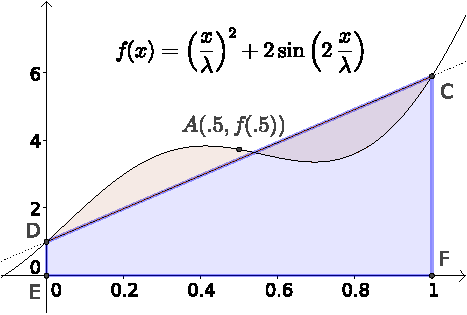
\includegraphics{figures/solutions01}
\par\end{center}

Luas trapesium $CDEF$ merepresentasikan hampiran dengan Aturan Trapesium
(yang menjadi asal namanya). Fungsi $f(x)$ dipilih sedemikian rupa
sehingga kedua daerah berwarna kecokelatan (hampir) sama luasnya,
satu di atas ruas garis $CD$ dan satu lagi di bawahnya. Ini berarti
hampiran Aturan Trapesium akan (hampir) eksak. Selain itu, karena
titik $A$ tidak terletak pada ruas garis $CD$, hampiran Aturan Simpson
tidak akan (hampir) eksak. Contoh lain dapat dibuat dengan cara serupa.
Ringkasnya, setiap contoh fungsi mulus yang memenuhi hal-hal berikut
dapat digunakan.
\begin{itemize}
\item Luas daerah di atas dan di bawah ruas garis dari $(0,f(0))$ hingga
$(1,f(1))$ sama.
\item $(.5,f(.5))$ tidak terletak pada ruas garis dari $(0,f(0))$ hingga
$(1,f(1))$.
\end{itemize}
\begin{description}
\item [{CATATAN:}] Fungsi tak mulus dengan kedua sifat di atas juga dapat
menjadi contoh. Kita memilih memberikan contoh mulus karena galat
untuk fungsi tak mulus sama sekali tidak dapat diperkirakan (karena
fungsi tersebut tidak memiliki banyaknya turunan yang diperlukan),
sehingga tidak terlalu mengejutkan jika dalam kasus itu kita dapat
menemukan contoh ketika Aturan Trapesium mengungguli Aturan Simpson.
Aturan Trapesium dan Aturan Simpson tidak dapat diterapkan secara
andal pada fungsi yang tidak memiliki turunan yang memadai.
\item [{CATATAN:}] Soal tidak meminta rumus, sehingga sebarang grafik sketsa
tangan yang digambar tangan dan memiliki kedua sifat di atas sudah
memadai. Namun, karena kita memiliki rumus, kita dapat menunjukkan
hasilnya secara numerik. Untuk fungsi $f$ yang digambarkan di atas,
\begin{eqnarray*}
\int_{0}^{1}f(x)dx & \approx & 3.443097449311693\\
\mbox{Aturan Trapesium}=\frac{f(0)+f(1)}{2} & \approx & 3.443097449311694\\
\mbox{Aturan Simpson}=\frac{f(0)+4f(.5)+f(1)}{6} & \approx & 3.632535470843161.
\end{eqnarray*}
\end{description}
\item [{\ref{exc:calculusErrors-16}:}] Rumus lima titik untuk turunan
orde $2$ memiliki suku galat $O(h^{3}f^{(5)}(\xi_{h}))$ atau $O(h^{4}f^{(6)}(\xi_{h}))$,
sehingga $E_{.1}=k(.1)^{3}f^{(5)}(\xi_{.1})$ atau $E_{.1}=k(.1)^{4}f^{(6)}(\xi_{.1})$
dan $E_{.02}=k(.02)^{3}f^{(5)}(\xi_{.02})$ atau $E_{.02}=k(.02)^{4}f^{(6)}(\xi_{.02})$.
Dengan mengasumsikan $f^{(5)}(\xi_{.1})\approx f^{(5)}(\xi_{.02})$
jika suku galatnya adalah $O(h^{3}f^{(5)}(\xi_{h}))$ atau bahwa $f^{(6)}(\xi_{.1})\approx f^{(6)}(\xi_{.02})$
jika suku galatnya adalah $O(h^{4}f^{(6)}(\xi_{h}))$, kita memperkirakan
\[
\frac{E_{.1}}{E_{.02}}=\frac{k(.1)^{3}f^{(5)}(\xi_{.1})}{k(.02)^{3}f^{(5)}(\xi_{.02})}\approx\left(\frac{.1}{.02}\right)^{3}=125
\]
atau 
\[
\frac{E_{.1}}{E_{.02}}=\frac{k(.1)^{4}f^{(6)}(\xi_{.1})}{k(.02)^{4}f^{(6)}(\xi_{.02})}\approx\left(\frac{.1}{.02}\right)^{4}=625.
\]
\end{description}

\section*{Bagian \ref{sec:Composite}}
\begin{description}
\item [{\ref{exc:calculus-composite}a:}] Bagi interval integrasi, $[1,3]$,
menjadi 3 subselang dengan panjang sama dan terapkan Aturan Titik
Tengah pada setiap subselang. Jumlah ketiga taksiran tersebut adalah
jawabannya.

\begin{center}
\begin{tabular}{cc}
interval & Aturan Titik Tengah\tabularnewline
\hline 
$[1,1+\frac{2}{3}]$ & $\frac{2}{3}\ln(\sin(1+\frac{1}{3}))\approx-0.0189755760325961$\tabularnewline
$[1+\frac{2}{3},2+\frac{1}{3}]$ & $\frac{2}{3}\ln(\sin(2))\approx-0.06338869073010707$\tabularnewline
$[2+\frac{1}{3},3]$ & $\frac{2}{3}\ln(\sin(2+\frac{2}{3}))\approx-0.5216503391783174$\tabularnewline
\end{tabular}
\par\end{center}

\begin{center}
\[
\int_{1}^{3}\ln(\sin(x))dx\approx-0.6040146059410205
\]
\par\end{center}
\item [{\ref{exc:calculus-composite-7}a:}] Bagi interval integrasi, $[1,3]$,
menjadi 3 subselang dengan panjang sama dan terapkan Aturan Trapesium
pada setiap subselang. Jumlah ketiga taksiran tersebut adalah jawabannya.

\begin{center}
\begin{tabular}{cc}
interval & Aturan Trapesium\tabularnewline
\hline 
$[1,1+\frac{2}{3}]$ & $\frac{1}{3}\left(\ln(\sin(1))+\ln(\sin(1+\frac{2}{3}))\right)\approx-0.05906878811071457$\tabularnewline
$[1+\frac{2}{3},2+\frac{1}{3}]$ & $\frac{1}{3}\left(\ln(\sin(1+\frac{2}{3}))+\ln(\sin(2+\frac{1}{3}))\right)\approx-0.1096099655624244$\tabularnewline
$[2+\frac{1}{3},3]$ & $\frac{1}{3}\left(\ln(\sin(2+\frac{1}{3}))+\ln(\sin(3))\right)\approx-0.7607906360781023$\tabularnewline
\end{tabular}
\par\end{center}

\begin{center}
\[
\int_{1}^{3}\ln(\sin(x))dx\approx-0.9294693897512412
\]
\par\end{center}
\item [{\ref{exc:calculus-composite-8}a:}] Bagi interval integrasi, $[1,3]$,
menjadi 3 subselang dengan panjang sama dan terapkan Aturan Simpson
pada setiap subselang. Jumlah ketiga taksiran tersebut adalah jawabannya.
Misalkan $f(x)=\ln(\sin(x))$.

\begin{center}
\begin{tabular}{cc}
interval & Aturan Simpson\tabularnewline
\hline 
$[1,1+\frac{2}{3}]$ & $\frac{1}{9}\left(f(1)+4f(1+\frac{1}{3})+f(1+\frac{2}{3})\right)\approx-0.03233998005863559$\tabularnewline
$[1+\frac{2}{3},2+\frac{1}{3}]$ & $\frac{1}{9}\left(f(1+\frac{2}{3})+4f(2)+f(2+\frac{1}{3})\right)\approx-0.0787957823408795$\tabularnewline
$[2+\frac{1}{3},3]$ & $\frac{1}{9}\left(f(2+\frac{1}{3})+4f(2+\frac{2}{3})+f(3)\right)\approx-0.6013637714782457$\tabularnewline
\end{tabular}
\par\end{center}

\begin{center}
\[
\int_{1}^{3}\ln(\sin(x))dx\approx-0.7124995338777608
\]
\par\end{center}
\item [{\ref{exc:calculus-composite-9}a:}] Bagi interval integrasi, $[1,3]$,
menjadi 3 subselang dengan panjang sama dan terapkan Aturan Simpson
$\frac{3}{8}$ pada setiap subselang. Jumlah ketiga taksiran tersebut
adalah jawabannya. Misalkan $f(x)=\ln(\sin(x))$.

\begin{center}
\begin{tabular}{cc}
interval & Aturan Simpson $\frac{3}{8}$\tabularnewline
\hline 
$[1,1+\frac{2}{3}]$ & $\frac{1}{12}\left(f(1)+3f(1+\frac{2}{9})+3f(1+\frac{4}{9})+f(1+\frac{2}{3})\right)\approx-0.03227403251196553$\tabularnewline
$[1+\frac{2}{3},2+\frac{1}{3}]$ & $\frac{1}{12}\left(f(1+\frac{2}{3})+3f(1+\frac{8}{9})+3f(2+\frac{1}{9})+f(2+\frac{1}{3})\right)\approx-0.07868946204953159$\tabularnewline
$[2+\frac{1}{3},3]$ & $\frac{1}{12}\left(f(2+\frac{1}{3})+3f(2+\frac{5}{9})+3f(2+\frac{7}{9})+f(3)\right)\approx-0.5965852934114506$\tabularnewline
\end{tabular}
\par\end{center}

\begin{center}
\[
\int_{1}^{3}\ln(\sin(x))dx\approx-0.7075487879729477
\]
\par\end{center}
\item [{\ref{exc:calculus-composite-10}a:}] Bagi interval integrasi, $[1,3]$,
menjadi 3 subselang dengan panjang sama dan terapkan aturan kuadratur
pada setiap subselang. Jumlah ketiga taksiran tersebut adalah jawabannya.
Misalkan $f(x)=\ln(\sin(x))$.

\begin{center}
\begin{tabular}{cc}
interval & Aturan Kuadratur\tabularnewline
\hline 
$[1,1+\frac{2}{3}]$ & $\frac{1}{3}\left(f(1+\frac{2}{9})+f(1+\frac{4}{9})\right)\approx-0.02334244731238252$\tabularnewline
$[1+\frac{2}{3},2+\frac{1}{3}]$ & $\frac{1}{3}\left(f(1+\frac{8}{9})+f(2+\frac{1}{9})\right)\approx-0.068382627545234$\tabularnewline
$[2+\frac{1}{3},3]$ & $\frac{1}{3}\left(f(2+\frac{5}{9})+f(2+\frac{7}{9})\right)\approx-0.5418501791892335$\tabularnewline
\end{tabular}
\par\end{center}

\begin{center}
\[
\int_{1}^{3}\ln(\sin(x))dx\approx-0.63357525404685
\]
\par\end{center}
\item [{\ref{exc:calculus-composite-11}:}] Aturan Trapesium yang diterapkan
pada $\int_{0}^{\pi}\sin^{4}x\,dx$ menghasilkan
\[
\frac{\pi}{2}\left(\sin^{4}(0)+\sin^{4}(\pi)\right)=0,
\]
yang memiliki galat absolut $\frac{3}{8}\pi$. Karena Aturan Trapesium
memiliki suku galat $O\left(\frac{1}{n^{2}}\right)$, membagi interval
integrasi menjadi $n$ subselang seharusnya mengurangi galat dengan
faktor sekitar $\frac{1}{n^{2}}$. Oleh karena itu, kita perlu menyelesaikan
persamaan ${\displaystyle \frac{\frac{3}{8}\pi}{n^{2}}=10^{-4}}$:
\begin{eqnarray*}
\frac{\frac{3}{8}\pi}{n^{2}} & = & 10^{-4}\\
\frac{\frac{3}{8}\pi}{10^{-4}} & = & n^{2}\\
\sqrt{\frac{\frac{3}{8}\pi}{10^{-4}}} & = & n\\
n & \approx & 108.5.
\end{eqnarray*}
Meningkatkan jumlah interval dengan faktor 109 seharusnya cukup. Karena
taksiran awal hanya menggunakan satu interval, kita perlu menggunakan
109 interval untuk mencapai akurasi $10^{-4}$ akurasi.
\item [{\ref{exc:calculus-composite-17}:}] Misalkan $S_{k}(a,b)$ berarti
menerapkan Aturan Simpson komposit pada interval $[a,b]$ dengan $k$
subselang dan $e_{k}$ menyatakan galat dalam $S_{k}(a,b)$. Kita
sekarang mengulangi analisis yang digunakan untuk menurunkan Aturan
Trapesium adaptif tetapi diterapkan pada Aturan Simpson: 
\[
e_{n}\approx M\left(\frac{1}{n}\right)^{4}\quad\mbox{dan}\quad e_{2n}\approx M\left(\frac{1}{2n}\right)^{4}
\]
sehingga
\begin{eqnarray*}
\frac{e_{n}}{e_{2n}} & \approx & \frac{M\left(\frac{1}{n}\right)^{4}}{M\left(\frac{1}{2n}\right)^{4}}=16,\quad\mbox{yang menyiratkan}\quad e_{n}\approx16e_{2n}.
\end{eqnarray*}
Karena $\int_{a}^{b}f(x)dx=S_{2}(a,b)+e_{2}=S_{1}(a,b)+e_{1}$,
\begin{eqnarray*}
S_{2}(a,b)-S_{1}(a,b) & = & e_{1}-e_{2}\\
 & \approx & 16e_{2}-e_{2}\\
 & = & 15e_{2}
\end{eqnarray*}
sehingga $e_{2}\approx\frac{1}{15}(S_{2}(a,b)-S_{1}(a,b)).$ Secara
eksplisit, 
\[
\int_{a}^{b}f(x)dx-S_{2}(a,b)\approx\frac{1}{15}(S_{2}(a,b)-S_{1}(a,b)).
\]
Sekarang kita tahu besaran yang digunakan untuk menaksir galat. Kita
menabelkan perhitungan yang diperlukan:

\begin{center}
\begin{tabular}{ccccccc}
$a$ & $b$ & $S_{1}(a,b)$ & $S_{2}(a,b)$ & $\frac{1}{15}\left|S_{2}(a,b)-S_{1}(a,b)\right|$ & $tol$ & \tabularnewline
\hline 
$1$ & $3$ & $-0.837026$ & $-0.730741$ & $0.00708$ & $.002$ & 
\includegraphics[scale=0.23]{figures/xMarkRed}\tabularnewline
$1$ & $2$ & $-0.046286$ & $-0.045560$ & $4.8(10)^{-5}$ & $.001$ & 
\includegraphics[scale=0.23]{figures/checkMarkGreen}\tabularnewline
2 & $3$ & $-0.684454$ & \textbf{$-0.661383$} & $0.00153$ & $.001$ & 
\includegraphics[scale=0.23]{figures/xMarkRed}\tabularnewline
$2$ & $2.5$ & $-0.134349$ & \textbf{$-0.134243$} & $7.0(10)^{-6}$ & $.0005$ & 
\includegraphics[scale=0.23]{figures/checkMarkGreen}\tabularnewline
$2.5$ & $3$ & $-0.527034$ & \textbf{$-0.523129$} & $0.00026$ & $.0005$ & 
\includegraphics[scale=0.23]{figures/checkMarkGreen}\tabularnewline
\hline 
\multicolumn{7}{c}{$\int_{1}^{3}\ln(\sin(x))dx\approx-0.045560-0.134243-0.523129=-0.702932$}\tabularnewline
\end{tabular}
\par\end{center}
\item [{\ref{exc:calculus-composite-12}:}] Pertama,
\begin{eqnarray*}
\int_{0}^{1}\ln(x+1)dx & = & \left[(x+1)\ln(x+1)-x-1\right]_{0}^{1}\\
 & = & 2\ln2-2-(-1)\\
 & = & 2\ln2-1\\
 & \approx & 0.3862943611198906.
\end{eqnarray*}
Sekarang kita perlu memperoleh taksiran menggunakan Aturan Trapesium
komposit dengan sejumlah kecil subselang, misalnya 10 atau 20. Bagian
perhitungan ini hanyalah perkiraan awal. Sebenarnya, berapa pun jumlah
subselang yang belum memberikan akurasi yang diinginkan sudah memadai:
\[
T_{10}(0,1)=0.385877936745754.
\]
Galat dengan 10 subselang adalah 
\[
|0.3862943611198906-0.385877936745754|\approx4.16424374136581(10)^{-4}.
\]
Karena suku galat untuk Aturan Trapesium komposit (dengan mengasumsikan
$f''(\xi_{h})$ konstan, sebagaimana dalam penurunan metode adaptif)
adalah $O\left(\frac{1}{n^{2}}\right)$, kita memperkirakan galat
berkurang dengan faktor $n^{2}$ ketika jumlah subselang diperbesar
dengan faktor $n$. Faktor penurunan yang diperlukan adalah
\[
\frac{10^{-6}}{4.16424374136581(10)^{-4}}\approx0.00240139641699267.
\]
Oleh karena itu, faktor peningkatan yang diperlukan adalah $\sqrt{\frac{1}{0.00240139641699267}}\approx20.406$.
Perhitungan ``uji'' kita menggunakan 10 subselang, sehingga kita
perlu menggunakan $10\cdot20.406=204.06$, atau jika dibulatkan ke
atas, $205$ subselang untuk mencapai akurasi $10^{-6}$.

\begin{description}
\item [{CATATAN:}] Cara lain untuk mencari faktor peningkatan yang diperlukan
adalah dengan menyelesaikan persamaan 
\[
\frac{4.16424374136581(10)^{-4}}{n^{2}}=10^{-6}.
\]
Hal ini berasal dari fakta bahwa memperbesar jumlah subselang dengan
faktor $n$ mengurangi galat dengan faktor $n^{2}$. Jadi, kita mengambil
galat yang diketahui (sebesar $T_{10}(0,1)$), membaginya dengan $n^{2}$
dan menyamakannya dengan akurasi yang diinginkan, $10^{-6}$. Solusinya
tentu saja adalah $n\approx20.406$, yaitu faktor peningkatannya.
\item [{CATATAN:}] Kita telah menggunakan kode Octave\index{Aturan Trapesium komposit!kode}\begin{verbatim}
####################################################
# Written by Dr. Len Brin           2 April 2012   #
# MAT 322 Numerical Analysis I                     #
# Purpose: Implementation of composite Trapezoidal #
# rule                                             #
# INPUT: function f, interval endpoints a and b,   #
#        number of subintervals n                  #
# OUTPUT: approximate integral of f(x) from a to b #
####################################################
function integral = compositeTrapezoidal(f,a,b,n)
  h = (b-a)/n;
  s = 0;
  for i = 1:n-1
    s = s + f(a+i*h);
  end#for
  integral = h*(f(a)+2*s+f(b))/2;
end#function
\end{verbatim}untuk menghitung $T_{10}(0,1)$:\begin{verbatim}
>> f=@(x) log(x+1);
>> compositeTrapezoidal(f,0,1,10)
ans =  0.385877936745754
\end{verbatim}\texttt{compositeTrapezoidal.m} dapat diunduh di \href{http://lqbrin.github.io/tea-time-numerical/ancillaries.html}{situs pendamping}.
\item [{CATATAN:}] Dengan menggunakan kode di atas untuk menghitung hampiran
dengan 205 subselang:\begin{verbatim}
>> compositeTrapezoidal(f,0,1,205)
ans =  0.386293369647938
\end{verbatim}dan galatnya adalah \begin{verbatim}
>> 0.3862943611198906-ans
ans =    9.91471952871414e-07
\end{verbatim}sedikit kurang dari $10^{-6}$.
\end{description}
\end{description}

\section*{Bagian \ref{sec:Extrapolation}}
\begin{description}
\item [{\ref{exc:calculus-extrapolation-5}:}] Kita perlu menggabungkan
$N(h)$, $N(\frac{h}{2})$, dan $N(\frac{h}{3})$ sehingga suku yang
memuat $h$ dan $h^{2}$ lenyap, menyisakan $h^{3}$ sebagai suku
berorde paling rendah.
\begin{eqnarray*}
N(h) & = & M-K_{1}h-K_{2}h^{2}-K_{3}h^{3}-\cdots\\
N\left(\frac{h}{2}\right) & = & M-\frac{1}{2}K_{1}h-\frac{1}{4}K_{2}h^{2}-\frac{1}{8}K_{3}h^{3}-\cdots\\
N\left(\frac{h}{3}\right) & = & M-\frac{1}{3}K_{1}h-\frac{1}{9}K_{2}h^{2}-\frac{1}{27}K_{3}h^{3}-\cdots
\end{eqnarray*}
sehingga $N(h)+aN(\frac{h}{2})+bN(\frac{h}{3})$ adalah
\[
(1+a+b)M-\left(1+\frac{a}{2}+\frac{b}{3}\right)K_{1}h-\left(1+\frac{a}{4}+\frac{b}{9}\right)K_{2}h^{2}-\left(1+\frac{a}{8}+\frac{b}{27}\right)K_{3}h^{3}-\cdots.
\]
Oleh karena itu, kita perlu mencari $a$ dan $b$ sedemikian sehingga
\begin{eqnarray*}
1+\frac{a}{2}+\frac{b}{3} & = & 0\\
1+\frac{a}{4}+\frac{b}{9} & = & 0.
\end{eqnarray*}
Solusi sistem tersebut adalah $a=-8$ dan $b=9$. Dengan menghitung,
\[
N(h)-8N\left(\frac{h}{2}\right)+9N\left(\frac{h}{3}\right)=2M+O(h^{3})
\]
sehingga taksiran $O(h^{3})$ kita untuk $M$ adalah
\[
\frac{N(h)-8N(\frac{h}{2})+9N(\frac{h}{3})}{2}.
\]

\begin{description}
\item [{CATATAN:}] Kita juga dapat bekerja langsung dengan ekstrapolasi
Richardson (setidaknya pada awalnya). Dengan menggunakan ekstrapolasi
Richardson dengan $\alpha=\frac{1}{2}$ dan $m_{1}=1$, kita dapat
menggabungkan $N(h)$ dan $N(\frac{h}{2})$ untuk memperoleh hampiran
$O(h^{2})$:
\[
N_{1}(h)=2N\left(\frac{h}{2}\right)-N(h).
\]
Dengan menggunakan ekstrapolasi Richardson dengan $\alpha=\frac{2}{3}$
dan $m_{1}=1$, kita dapat menggabungkan $N(\frac{h}{2})$ dan $N(\frac{h}{3})$
untuk memperoleh hampiran $O(h^{2})$ lainnya: 
\begin{eqnarray*}
\hat{N}_{1}\left(\frac{h}{2}\right) & = & \frac{\frac{3}{2}N(\frac{h}{3})-N(\frac{h}{2})}{\frac{1}{2}}\\
 & = & 3N\left(\frac{h}{3}\right)-2N\left(\frac{h}{2}\right).
\end{eqnarray*}
Baik $N_{1}$ maupun $\hat{N}_{1}$ merupakan hampiran $O(h^{2})$
sehingga keduanya dapat digabungkan untuk memperoleh hampiran $O(h^{3})$.
Sayangnya, rumus ekstrapolasi Richardson tidak berlaku. Rumus tersebut
mengasumsikan konstanta yang sama pada setiap hampiran. Namun, gagasan
umumnya tetap berlaku. Kita perlu menggabungkan hampiran-hampiran
ini
\begin{eqnarray*}
N_{1}(h) & = & M+\frac{1}{2}K_{2}h^{2}+\frac{3}{4}K_{3}h^{3}+\cdots\\
\hat{N}_{1}\left(\frac{h}{2}\right) & = & M+\frac{1}{6}K_{2}h^{2}+\frac{5}{36}K_{3}h^{3}+\cdots
\end{eqnarray*}
untuk menghilangkan suku $h^{2}$. Dengan mengamati bentuknya, kita
memerlukan $3\hat{N}_{1}(\frac{h}{2})-N_{1}(h)$: 
\[
3\hat{N}_{1}\left(\frac{h}{2}\right)-N_{1}(h)=2M-\frac{1}{3}K_{3}h^{3}-\cdots.
\]
 Oleh karena itu, hampiran $O(h^{3})$ untuk $M$ yang kita cari adalah
\begin{eqnarray*}
N_{2}(h) & = & \frac{3\hat{N}_{1}(\frac{h}{2})-N_{1}(h)}{2}\\
 & = & \frac{3\left[3N(\frac{h}{3})-2N(\frac{h}{2})\right]-\left[2N(\frac{h}{2})-N(h)\right]}{2}\\
 & = & \frac{N(h)-8N(\frac{h}{2})+9N(\frac{h}{3})}{2}.
\end{eqnarray*}
\end{description}
\item [{\ref{exc:calculus-extrapolation-6}:}] Untuk ekstrapolasi pertama,
kita menggunakan rumus \ref{eq:richardsonBasis} dengan $\alpha=\frac{1}{2}$
dan $m_{1}=2$:
\[
N_{1}(h)=\frac{4N(\frac{h}{2})-N(h)}{3},
\]
yang menyisakan $N_{1}(h)=M+l_{2}h^{4}+l_{3}h^{6}+\cdots$. Penyempurnaan
tahap kedua diperoleh dari rumus \ref{eq:richardsonBasis} dengan
$\alpha=\frac{1}{2}$ dan $m_{1}=4$:
\[
N_{2}(h)=\frac{16N_{1}(\frac{h}{2})-N_{1}(h)}{15},
\]
yang menyisakan $N_{2}(h)=M+c_{3}h^{6}+\cdots$. Penyempurnaan tahap
ketiga diperoleh dari rumus \ref{eq:richardsonBasis} dengan $\alpha=\frac{1}{2}$
dan $m_{1}=6$:
\[
N_{3}(h)=\frac{64N_{2}(\frac{h}{2})-N_{2}(h)}{63}.
\]
Jika perhitungan ditabulasikan, hasilnya kira-kira sebagai berikut:

\begin{center}
\begin{tabular}{cccc}
$N$ & $N_{1}$ & $N_{2}$ & $N_{3}$\tabularnewline
\hline 
$2.356194$ &  &  & \tabularnewline
$-0.4879837$ & $-1.436042$ &  & \tabularnewline
$-0.8815732$ & $-1.012769$ & $-0.9845514$ & \tabularnewline
$-0.9709157$ & $-1.000696$ & $-0.9998916$ & $-1.000135$\tabularnewline
\end{tabular}
\par\end{center}

Ekstrapolasi Richardson ketiga adalah $-1.000135$. Hasil ini cukup
baik mengingat nilai eksak integral tersebut adalah $-1$.
\item [{\ref{exc:calculus-extrapolation-11}a:}] Untuk merangkum metode
ini, misalkan $N_{0}(k)=T_{k}(1,3)$, yaitu Aturan Trapesium itu sendiri
yang diterapkan dengan $k$ subselang. Karena galat Aturan Trapesium
hanya memuat pangkat genap, 
\[
N_{j}(k)=\frac{4^{j}N_{j-1}(2k)-N_{j-1}(k)}{4^{j}-1}
\]
untuk $j=1,2,\ldots$. Hingga enam angka signifikan, tabel berikut
merangkum prosesnya.\\
\\
\begin{tabular}{c|ccccccc}
$k$ & $N_{0}(k)$ & $N_{1}(k)$ & $N_{2}(k)$ & $N_{3}(k)$ & $N_{4}(k)$ & $N_{5}(k)$ & $N_{6}(k)$\tabularnewline
\hline 
$1$ & $-2.13074$ & $-0.837026$ & $-0.723655$ & $-0.705067$ & $-0.702555$ & $-0.702340$ & $-0.702330$\tabularnewline
$2$ & $-1.16045$ & $-0.730741$ & $-0.705358$ & $-0.702564$ & $-0.702340$ & $-0.702330$ & \tabularnewline
$4$ & $-0.838170$ & $-0.706944$ & $-0.702608$ & $-0.702341$ & $-0.702330$ &  & \tabularnewline
$8$ & $-0.739751$ & $-0.702879$ & $-0.702345$ & $-0.702330$ &  &  & \tabularnewline
$16$ & $-0.712097$ & $-0.702378$ & $-0.702330$ &  &  &  & \tabularnewline
$32$ & $-0.704808$ & $-0.702333$ &  &  &  &  & \tabularnewline
$64$ & $-0.702952$ &  &  &  &  &  & \tabularnewline
\end{tabular}\\
\\
Hingga akurasi mesin (Octave),
\[
\int_{1}^{3}\ln(\sin(x))dx\approx-0.702330215031025
\]
\end{description}

\section*{Bagian \ref{sec:Splines}}
\begin{description}
\item [{\ref{exc:cubicSplines}:}] Karena diberikan tiga titik, splin tersebut
terdiri atas dua bagian kubik. Setiap bagian kubik memiliki 4 koefisien,
sehingga kita perlu menyusun sistem 8 persamaan dengan 8 peubah tak
diketahui. Splin $S$ berbentuk
\[
S(x)=\begin{cases}
S_{1}(x)=a_{1}+b_{1}(x-1)+c_{1}(x-1)^{2}+d_{1}(x-1)^{3}, & x\in[0,1]\\
S_{2}(x)=a_{2}+b_{2}(x-2)+c_{2}(x-2)^{2}+d_{2}(x-2)^{3}, & x\in[1,2]
\end{cases}.
\]
Kedelapan persamaan berasal dari tiga kelompok syarat bagi setiap
splin kubik bebas.\\
Interpolasi:

\begin{itemize}
\item $S_{1}(0)=-9\Rightarrow a_{1}-b_{1}+c_{1}-d_{1}=-9$
\item $S_{1}(1)=-13\Rightarrow a_{1}=-13$
\item $S_{2}(1)=-13\Rightarrow a_{2}-b_{2}+c_{2}-d_{2}=-13$
\item $S_{2}(2)=-29\Rightarrow a_{2}=-29$
\end{itemize}
Kecocokan turunan:
\begin{itemize}
\item $S_{1}'(1)=S_{2}'(1)\Rightarrow b_{1}=b_{2}-2c_{2}+3d_{2}$
\item $S_{1}''(1)=S_{2}''(1)\Rightarrow2c_{1}=2c_{2}-6d_{2}$
\end{itemize}
Syarat titik ujung:
\begin{itemize}
\item $S_{1}''(0)=0\Rightarrow2c_{1}-6d_{1}=0$
\item $S_{2}''(2)=0\Rightarrow2c_{2}=0$
\end{itemize}
\item [{\ref{exc:cubicSplines-4}:}] Karena diberikan tiga titik, splin
tersebut terdiri atas dua bagian kubik. Setiap bagian kubik memiliki
4 koefisien, sehingga kita perlu menyusun sistem 8 persamaan dengan
8 peubah tak diketahui. Splin $S$ berbentuk
\[
S(x)=\begin{cases}
S_{1}(x)=a_{1}+b_{1}(x-2)+c_{1}(x-2)^{2}+d_{1}(x-2)^{3}, & x\in[1,2]\\
S_{2}(x)=a_{2}+b_{2}(x-4)+c_{2}(x-4)^{2}+d_{2}(x-4)^{3}, & x\in[2,4]
\end{cases}.
\]
Kedelapan persamaan berasal dari tiga kelompok syarat bagi setiap
splin kubik terkekang.\\
Interpolasi:

\begin{itemize}
\item $S_{1}(1)=1\Rightarrow a_{1}-b_{1}+c_{1}-d_{1}=1$
\item $S_{1}(2)=3\Rightarrow a_{1}=3$
\item $S_{2}(2)=3\Rightarrow a_{2}-2b_{2}+4c_{2}-8d_{2}=3$
\item $S_{2}(4)=2\Rightarrow a_{2}=2$
\end{itemize}
Kecocokan turunan:
\begin{itemize}
\item $S_{1}'(2)=S_{2}'(2)\Rightarrow b_{1}=b_{2}-4c_{2}+12d_{2}$
\item $S_{1}''(2)=S_{2}''(2)\Rightarrow2c_{1}=2c_{2}-12d_{2}$
\end{itemize}
Syarat titik ujung:
\begin{itemize}
\item $S_{1}'(1)=0\Rightarrow b_{1}-2c_{1}+3d_{1}=0$
\item $S_{2}'(4)=0\Rightarrow b_{2}=0$
\end{itemize}
\item [{\ref{exc:cubicSplines-6}:}] Dengan mengikuti penyelesaian yang
diuraikan dalam teks, persamaan \ref{eq:firstNm2} memberikan $n-2=0$
persamaan dalam peubah $c_{i}$. Persamaan \ref{eq:finalEquation}
memberikan $-4c_{1}-2c_{2}=3\left(\frac{4}{-1}-\frac{16}{-1}\right)$,
yang disederhanakan menjadi 
\[
-4c_{1}-2c_{2}=36.
\]
Jika digabungkan dengan persamaan $c_{2}=0$, diperoleh $c_{1}=-9$.
Sekarang kita telah memperoleh nilai $a_{i}$ dan $c_{i}$. Bagian
penyelesaian selanjutnya hanyalah substitusi balik. Dari kondisi titik
ujung kiri, $d_{1}=\frac{1}{3}c_{1}=-3$. Dari kecocokan turunan kedua,
$d_{2}=\frac{c_{2}-c_{1}}{3}=\frac{0-(-9)}{3}=3$. Sekarang kita telah
memperoleh nilai $d_{i}$. Dari syarat interpolasi, $b_{1}=a_{1}+c_{1}-d_{1}+9$
dan $b_{2}=a_{2}+c_{2}-d_{2}+13$, sehingga 
\begin{eqnarray*}
b_{1} & = & -13-9+3+9=-10\\
b_{2} & = & -29+0-3+13=-19.
\end{eqnarray*}
Dengan demikian, splinnya adalah
\[
S(x)=\begin{cases}
-13-10(x-1)-9(x-1)^{2}-3(x-1)^{3}, & x\in[0,1]\\
-29-19(x-2)+3(x-2)^{3}, & x\in[1,2].
\end{cases}
\]

\begin{description}
\item [{CATATAN:}] Penyelesaian yang diuraikan dalam teks bukan satu-satunya
cara untuk memperoleh solusi. Metode apa pun untuk menyelesaikan enam
persamaan yang memuat $b_{i}$, $c_{i}$, dan $d_{i}$ dapat digunakan.
\end{description}
\item [{\ref{exc:cubicSplines-11}:}] Dengan mengikuti penyelesaian yang
diuraikan dalam teks, persamaan \ref{eq:firstNm2} memberikan $n-2=0$
persamaan dalam peubah $c_{i}$. Kita tidak dapat menggunakan persamaan
\ref{eq:finalEquation} karena persamaan tersebut diturunkan dari
syarat titik ujung bebas. Sebagai gantinya, kita perlu menggunakan
syarat titik ujung terkekang untuk memperoleh dua persamaan dalam
peubah $c_{i}$. Persamaan \ref{eq:b1} memberikan $b_{1}=\frac{1}{-2}+\frac{-4}{3}c_{1}+\frac{-2}{3}c_{2}$.
Dengan menyelesaikan persamaan kecocokan turunan kedua untuk $d_{2}$,
diperoleh $d_{2}=\frac{c_{2}-c_{1}}{6}$. Dengan menyubstitusikan
bentuk untuk $b_{1}$, $b_{2}$, dan $d_{2}$ ke persamaan kecocokan
turunan pertama, $\frac{1}{-2}=-\frac{2}{3}c_{1}-\frac{4}{3}c_{2}$,
yang disederhanakan menjadi $4c_{1}+8c_{2}=3$. Ini adalah persamaan
pertama kita dalam peubah $c_{i}$. Sekarang, dengan menyelesaikan
kondisi titik ujung kiri untuk $d_{1}$, diperoleh $d_{1}=\frac{2c_{1}-b_{1}}{3}$.
Dengan menyubstitusikan bentuk untuk $a_{1}$, $b_{1}$, dan $d_{1}$
ke persamaan interpolasi pertama, diperoleh $3-(\frac{1}{-2}+\frac{-4}{3}c_{1}+\frac{-2}{3}c_{2})+c_{1}-\frac{2c_{1}-(\frac{1}{-2}+\frac{-4}{3}c_{1}+\frac{-2}{3}c_{2})}{3}=1$,
yang disederhanakan menjadi $11c_{1}+4c_{2}=-21$. Kedua persamaan
dalam peubah $c_{i}$ kini dapat diselesaikan untuk mencari $c_{1}=-\frac{5}{2}$
dan $c_{2}=\frac{13}{8}$. Seperti pada splin bebas, bagian penyelesaian
selanjutnya hanyalah substitusi balik: 
\begin{eqnarray*}
b_{1} & = & \frac{1}{-2}+\frac{-4}{3}\left(-\frac{5}{2}\right)+\frac{-2}{3}\left(\frac{13}{8}\right)=\frac{7}{4}\\
d_{1} & = & \frac{2(-\frac{5}{2})-\frac{7}{4}}{3}=-\frac{9}{4}\\
d_{2} & = & \frac{\frac{13}{8}-\left(-\frac{5}{2}\right)}{6}=\frac{11}{16}.
\end{eqnarray*}
Dengan demikian, splinnya adalah
\[
S(x)=\begin{cases}
3+\frac{7}{4}(x-2)-\frac{5}{2}(x-2)^{2}-\frac{9}{4}(x-2)^{3}, & x\in[1,2]\\
2+\frac{13}{8}(x-4)^{2}+\frac{11}{16}(x-4)^{3}, & x\in[2,4].
\end{cases}
\]

\begin{description}
\item [{CATATAN:}] Penyelesaian yang diuraikan dalam teks bukan satu-satunya
cara untuk memperoleh solusi. Metode apa pun untuk menyelesaikan enam
persamaan yang memuat $b_{i}$, $c_{i}$, dan $d_{i}$ dapat digunakan.
\end{description}
\item [{\ref{exc:cubicSplines-14}:}] \begin{verbatim}
>> [a,b,c,d]=naturalCubicSpline([0,1,2],[-9,-13,-29])
a =
  -13  -29

b =
  -10  -19

c =
  -9   0

d =
  -3   3
\end{verbatim}
\item [{\ref{exc:cubicSplines-9}:}] Pertama, deklarasi fungsi harus diubah.
Turunan di titik ujung kiri dan kanan, $m_{0}$ dan $m_{n}$, akan
ditentukan, sehingga fungsi tersebut memerlukan argumen tambahan.
Selain itu, nama fungsi perlu diubah:\begin{verbatim}
function [a,b,c,d] = naturalCubicSpline(x,y)
\end{verbatim}harus menjadi\begin{verbatim}
function [a,b,c,d] = clampedCubicSpline(x,y,m0,mn)
\end{verbatim}Modifikasi selanjutnya melibatkan syarat titik ujung dan pengaruhnya
terhadap persamaan di dalam fungsi. Kita mulai dengan menyelesaikan
kondisi titik ujung kiri untuk $d_{1}$: $b_{1}+2c_{1}h_{1}+3d_{1}h_{1}^{2}=m_{0}\Rightarrow$
\begin{equation}
d_{1}=\frac{m_{0}-b_{1}-2c_{1}h_{1}}{3h_{1}^{2}}.\label{eq:d1}
\end{equation}
Dengan menyubstitusikan persamaan ini, $a_{i}=y_{i}$, serta persamaan
\ref{eq:b1} ke dalam \ref{eq:interpolationRequirement} dengan $i=1$
diperoleh 
\[
y_{1}+\left(\frac{y_{1}-y_{2}}{h_{2}}+\frac{2}{3}h_{2}c_{1}+\frac{1}{3}h_{2}c_{2}\right)h_{1}+c_{1}h_{1}^{2}+\frac{m_{0}-\left(\frac{y_{1}-y_{2}}{h_{2}}+\frac{2}{3}h_{2}c_{1}+\frac{1}{3}h_{2}c_{2}\right)-2c_{1}h_{1}}{3h_{1}^{2}}h_{1}^{3}=y_{0},
\]
yang disederhanakan sebagai berikut.
\begin{eqnarray*}
\left(\frac{y_{1}-y_{2}}{h_{2}}+\frac{2}{3}h_{2}c_{1}+\frac{1}{3}h_{2}c_{2}\right)h_{1}+c_{1}h_{1}^{2}+\frac{m_{0}-\left(\frac{y_{1}-y_{2}}{h_{2}}+\frac{2}{3}h_{2}c_{1}+\frac{1}{3}h_{2}c_{2}\right)-2c_{1}h_{1}}{3}h_{1} & = & y_{0}-y_{1}\\
\frac{y_{1}-y_{2}}{h_{2}}+\frac{2}{3}h_{2}c_{1}+\frac{1}{3}h_{2}c_{2}+c_{1}h_{1}+\frac{m_{0}-\left(\frac{y_{1}-y_{2}}{h_{2}}+\frac{2}{3}h_{2}c_{1}+\frac{1}{3}h_{2}c_{2}\right)-2c_{1}h_{1}}{3} & = & \frac{y_{0}-y_{1}}{h_{1}}\\
3\frac{y_{1}-y_{2}}{h_{2}}+2h_{2}c_{1}+h_{2}c_{2}+3c_{1}h_{1}+m_{0}-\left(\frac{y_{1}-y_{2}}{h_{2}}+\frac{2}{3}h_{2}c_{1}+\frac{1}{3}h_{2}c_{2}\right)+-2c_{1}h_{1} & = & 3\frac{y_{0}-y_{1}}{h_{1}}\\
2\frac{y_{1}-y_{2}}{h_{2}}+2h_{2}c_{1}+h_{2}c_{2}+c_{1}h_{1}+m_{0}-\left(\frac{2}{3}h_{2}c_{1}+\frac{1}{3}h_{2}c_{2}\right) & = & 3\frac{y_{0}-y_{1}}{h_{1}}\\
6\frac{y_{1}-y_{2}}{h_{2}}+6h_{2}c_{1}+3h_{2}c_{2}+3c_{1}h_{1}+3m_{0}-\left(2h_{2}c_{1}+h_{2}c_{2}\right) & = & 9\frac{y_{0}-y_{1}}{h_{1}}\\
6\frac{y_{1}-y_{2}}{h_{2}}+4h_{2}c_{1}+2h_{2}c_{2}+3c_{1}h_{1}+3m_{0} & = & 9\frac{y_{0}-y_{1}}{h_{1}},
\end{eqnarray*}
dan akhirnya 
\begin{equation}
\left(4h_{2}+3h_{1}\right)c_{1}+2h_{2}c_{2}=9\frac{y_{0}-y_{1}}{h_{1}}-6\frac{y_{1}-y_{2}}{h_{2}}-3m_{0}.\label{eq:firstC}
\end{equation}
Kondisi titik ujung kanan, $S_{n}'(x_{n})=m_{n}$ memberikan $b_{n}=m_{n}$.
Dengan menyubstitusikan informasi ini ke dalam \ref{eq:bi} dengan
$i=n$ diperoleh $m_{n}=\frac{y_{n-1}-y_{n}}{h_{n}}-\frac{(c_{n-1}+2c_{n})h_{n}}{3}$,
yang disederhanakan menjadi
\begin{equation}
h_{n}c_{n-1}+2h_{n}c_{n}=3\left(\frac{y_{n-1}-y_{n}}{h_{n}}-m_{n}\right).\label{eq:secondC}
\end{equation}
Persamaan \ref{eq:firstC} harus diterapkan dalam kode yang dimodifikasi
pada baris 21 dan 22: \begin{verbatim}
  m(1,1)=2*(h(1)+h(2)); m(1,2)=h(2);
  m(1,n+1)=3*((y(1)-y(2))/h(1)-(y(2)-y(3))/h(2)); 
\end{verbatim}menjadi\begin{verbatim}
  m(1,1)=3*h(1)+4*h(2); m(1,2)=2*h(2);
  m(1,n+1)=9*(y(1)-y(2))/h(1)-6*(y(2)-y(3))/h(2)-3*m0; 
\end{verbatim} Persamaan \ref{eq:secondC} harus diterapkan dalam kode yang dimodifikasi
pada baris 25:\begin{verbatim}
  m(n,n-1)=0; m(n,n)=1; m(n,n+1)=0;
\end{verbatim}menjadi\begin{verbatim}
  m(n,n-1)=h(n); m(n,n)=2*h(n); m(n,n+1)=3*((y(n)-y(n+1))/h(n)-mn);
\end{verbatim} Penyelesaian untuk nilai $c_{i}$ tetap tidak berubah. Kita hanya
perlu memodifikasi perhitungan $b_{1}$ dan $d_{1}$ pada baris 47
dan 48. $b_{1}$ kini berasal dari \ref{eq:b1}, sehingga \begin{verbatim}
  b(1)=(y(1)-y(2))/h(1)-2*c(1)*h(1)/3;
\end{verbatim}menjadi\begin{verbatim}
  b(1)=(y(2)-y(3))/h(2)+2*c(1)*h(2)/3+h(2)*c(2)/3;
\end{verbatim}$d_{1}$ kini berasal dari \ref{eq:d1}, sehingga\begin{verbatim}
  d(1)=-c(1)/(3*h(1));
\end{verbatim}menjadi\begin{verbatim}
  d(1)=(m0-b(1)-2*c(1)*h(1))/(3*h(1)^2);
\end{verbatim}Tentu saja, komentar pada awal fungsi juga harus diperbarui. Dengan
demikian, kode yang dimodifikasi akan tampak kira-kira seperti ini:\begin{verbatim}
%%%%%%%%%%%%%%%%%%%%%%%%%%%%%%%%%%%%%%%%%%%%%%%%%
% Written by Dr. Len Brin           3 June 2014 %
% Purpose: Calculation of a natural cubic       %
%        spline.                                %
% INPUT: points (x(1),y(1)), (x(2),y(2)), ...   %
%        spline must interpolate; first         %
%        derivative at left endpoint, m0; first %
%        derivative at right endpoint, mn.      %
% OUTPUT: coefficients of each piece of the     %
%        piecewise cubic spline:                %
%        S(i,x) = a(i)                          %
%          + b(i)*(x-x(i+1))                    %
%          + c(i)*(x-x(i+1))^2                  %
%          + d(i)*(x-x(i+1))^3                  %
%%%%%%%%%%%%%%%%%%%%%%%%%%%%%%%%%%%%%%%%%%%%%%%%%
function [a,b,c,d] = clampedCubicSpline(x,y,m0,mn)
  n=length(x)-1;
  for i=1:n
    h(i)=x(i)-x(i+1);
  end%for
  % Left endpoint condition:
  % m(1,1)*c(1) + m(1,2)*c(2) = m(1,n+1)
  m(1,1)=3*h(1)+4*h(2); m(1,2)=2*h(2);
  m(1,n+1)=9*(y(1)-y(2))/h(1)-6*(y(2)-y(3))/h(2)-3*m0;
  % Right endpoint condition:
  % m(n,n-1)*c(n-1) + m(n,n)*c(n) = m(n,n+1)
  m(n,n-1)=h(n); m(n,n)=2*h(n); m(n,n+1)=3*((y(n)-y(n+1))/h(n)-mn);
  % Conditions for all splines:
  for i=2:n-1
    m(i,i-1)=h(i);
    m(i,i)=2*(h(i)+h(i+1));
    m(i,i+1)=h(i+1);
    m(i,n+1)=3*((y(i)-y(i+1))/h(i)-(y(i+1)-y(i+2))/h(i+1));
  end%for
  % Solve for c(i)
  l(1)=m(1,1); u(1)=m(1,2)/l(1); z(1)=m(1,n+1)/l(1);
  for i=2:n-1
    l(i)=m(i,i)-m(i,i-1)*u(i-1);
    u(i)=m(i,i+1)/l(i);
    z(i)=(m(i,n+1)-m(i,i-1)*z(i-1))/l(i);
  end%for
  l(n)=m(n,n)-m(n,n-1)*u(n-1);
  c(n)=(m(n,n+1)-m(n,n-1)*z(n-1))/l(n);
  for i=n-1:-1:1
    c(i)=z(i)-u(i)*c(i+1);
  end%for
  % Compute a(i), b(i), d(i)
  % Endpoint conditions:
  b(1)=(y(2)-y(3))/h(2)+2*c(1)*h(2)/3+h(2)*c(2)/3;
  d(1)=(m0-b(1)-2*c(1)*h(1))/(3*h(1)^2);
  % Conditions for all splines:
  a(1)=y(2);
  for i=2:n
    d(i)=(c(i-1)-c(i))/(3*h(i));
    b(i)=(y(i)-y(i+1))/h(i)-(c(i-1)+2*c(i))*h(i)/3;
    a(i)=y(i+1);
  end%for
  b(n)=mn;
end%function
\end{verbatim}Perhatikan penambahan perhitungan terakhir, \texttt{b(n)=mn}. Nilai
\texttt{b(n)} dari perulangan dapat terkena galat titik-mengambang.
Dengan menetapkan $b_{n}$ sama dengan $m_{n}$ pada akhir program,
variasi yang mungkin timbul ini dapat dihilangkan. \texttt{clampedCubicSpline.m}
dapat diunduh di \href{http://lqbrin.github.io/tea-time-numerical/ancillaries.html}{situs pendamping}.
\item [{\ref{exc:cubicSplines-16}:}] \begin{verbatim}
>> [a,b,c,d]=clampedCubicSpline([1,2,4],[1,3,2],0,0)
a =
   3   2

b =
   1.75000   0.00000

c =
  -2.5000   1.6250

d =
  -2.25000   0.68750
\end{verbatim}
\end{description}

\section*{Bagian \ref{sec:OdePendulum}}
\begin{description}
\item [{\ref{exc:odePendulum-2}:}] Derajat persamaan diferensial sama
dengan derajat pangkat tertinggi turunan dalam persamaan tersebut.
Satu-satunya turunan yang muncul dalam persamaan adalah suku $f'$.
Dengan demikian, pangkat tertinggi turunannya adalah 1, sehingga derajat
persamaan diferensial tersebut adalah 1.
\item [{\ref{exc:odePendulum-6}:}] Dalam persamaan diferensial $f'+\frac{f}{x}=x^{2}$,
baik $f$ maupun $f'$ muncul. Untuk memverifikasi bahwa fungsi $f$
merupakan solusi, kita perlu menyubstitusikan $f$ dan $f'$ ke dalam
persamaan. $f'$ tidak diberikan, sehingga kita menghitungnya:
\[
f'(x)=\frac{3x^{2}}{4}-\frac{4}{x^{2}}.
\]
Setelah semua yang diperlukan tersedia, kita menyubstitusikan $f$
dan $f'$ ke dalam persamaan diferensial dan memverifikasi kebenaran
persamaan tersebut. Dengan menyubstitusikan:
\begin{eqnarray*}
\left(\frac{3x^{2}}{4}-\frac{4}{x^{2}}\right)+\frac{\left(\frac{x^{3}}{4}+\frac{4}{x}\right)}{x} & = & x^{2}.
\end{eqnarray*}
Kebenaran persamaan ini belum tampak jelas, sehingga masih diperlukan
sedikit pekerjaan. Untuk menyelesaikan verifikasi, kita harus menunjukkan
secara aljabar bahwa kedua ruasnya sama. Menambah, mengurangi, atau
melakukan operasi lain pada kedua ruas secara bersamaan mengandaikan
bahwa kedua ruas itu sama, sehingga hal tersebut tidak diperbolehkan!
Sebagai gantinya, kedua ruas harus dimanipulasi secara terpisah. Dengan
mengolah ruas kiri saja:
\begin{eqnarray*}
\left(\frac{3x^{4}}{4x^{2}}-\frac{16}{4x^{2}}\right)+\left(\frac{x^{3}}{4x}+\frac{4}{x^{2}}\right) & = & x^{2}\\
\frac{3x^{4}}{4x^{2}}-\frac{16}{4x^{2}}+\frac{x^{4}}{4x^{2}}+\frac{16}{4x^{2}} & = & x^{2}\\
\frac{4x^{4}}{4x^{2}} & = & x^{2}.
\end{eqnarray*}
Hampir selesai, tetapi secara teknis persamaan ini tidak selalu benar!
Persamaan ini salah ketika $x=0$ karena ruas kiri tidak terdefinisi
untuk $x=0$. Untungnya, kasus tersebut tidak perlu kita khawatirkan.
Diberikan bahwa $x>0$, sehingga kita mengetahui $x\neq0$ dan kita
dapat menyederhanakan $\frac{4x^{4}}{4x^{2}}$ menjadi $x^{2}$, yang
menyelesaikan verifikasi.
\item [{\ref{exc:odePendulum-10}:}] Untuk memverifikasi bahwa suatu fungsi
merupakan solusi masalah nilai awal, kita perlu memastikan bahwa fungsi
itu memenuhi persamaan diferensial dan syarat nilai awal. 

\begin{itemize}
\item Menunjukkan bahwa $f(x)=\frac{x^{3}}{4}+\frac{16}{x}$, $x>0$, merupakan
solusi dari $f'=-\frac{f}{x}+x^{2}$: Dalam persamaan diferensial
$f'+\frac{f}{x}=x^{2}$, baik $f$ maupun $f'$ muncul. Untuk memverifikasi
bahwa fungsi $f$ merupakan solusi, kita perlu menyubstitusikan $f$
dan $f'$ ke dalam persamaan. $f'$ tidak diberikan, sehingga kita
menghitungnya:
\[
f'(x)=\frac{3x^{2}}{4}-\frac{16}{x^{2}}.
\]
Setelah semua yang diperlukan tersedia, kita menyubstitusikan $f$
dan $f'$ ke dalam persamaan diferensial dan memverifikasi kebenaran
persamaan tersebut. Dengan menyubstitusikan:
\begin{eqnarray*}
\left(\frac{3x^{2}}{4}-\frac{16}{x^{2}}\right)+\frac{\left(\frac{x^{3}}{4}+\frac{16}{x}\right)}{x} & = & x^{2}.
\end{eqnarray*}
Kebenaran persamaan ini belum tampak jelas, sehingga masih diperlukan
sedikit pekerjaan. Untuk menyelesaikan verifikasi, kita harus menunjukkan
secara aljabar bahwa kedua ruasnya sama. Menambah, mengurangi, atau
melakukan operasi lain pada kedua ruas secara bersamaan mengandaikan
bahwa kedua ruas itu sama, sehingga hal tersebut tidak diperbolehkan!
Sebagai gantinya, kedua ruas harus dimanipulasi secara terpisah. Dengan
mengolah ruas kiri saja:
\begin{eqnarray*}
\left(\frac{3x^{4}}{4x^{2}}-\frac{64}{4x^{2}}\right)+\left(\frac{x^{3}}{4x}+\frac{16}{x^{2}}\right) & = & x^{2}\\
\frac{3x^{4}}{4x^{2}}-\frac{64}{4x^{2}}+\frac{x^{4}}{4x^{2}}+\frac{64}{4x^{2}} & = & x^{2}\\
\frac{4x^{4}}{4x^{2}} & = & x^{2}.
\end{eqnarray*}
Hampir selesai, tetapi secara teknis persamaan ini tidak selalu benar!
Persamaan ini salah ketika $x=0$ karena ruas kiri tidak terdefinisi
untuk $x=0$. Untungnya, kasus tersebut tidak perlu kita khawatirkan.
Diberikan bahwa $x>0$, sehingga kita mengetahui $x\neq0$ dan kita
dapat menyederhanakan $\frac{4x^{4}}{4x^{2}}$ menjadi $x^{2}$, yang
menyelesaikan verifikasi.
\item Menunjukkan bahwa $f(4)=20$: Untuk menunjukkan bahwa $f$ memenuhi
syarat nilai awal, kita cukup menghitung $f(4)$ dan menunjukkan bahwa
nilainya 20 sebagaimana disyaratkan. $f(4)=\frac{4^{3}}{4}+\frac{16}{4}=\frac{64}{4}+\frac{16}{4}=\frac{80}{4}=20$.
\end{itemize}
\item [{\ref{exc:odePendulum-13}:}] Bentuk $\dot{y}=t-\sin t$ yang diberikan
dapat ditulis ulang sebagai $y'(t)=t-\sin t$. Dengan kata lain, kita
diberi turunan $y$ sebagai fungsi dari $t$. Teorema dasar kalkulus
menyatakan bahwa $y$ harus merupakan integral (antiturunan) dari
fungsi yang diberikan. Artinya,
\begin{eqnarray*}
y(t) & = & \int(t-\sin t)dt\\
 & = & \frac{1}{2}t^{2}+\cos t+C.
\end{eqnarray*}
Jadi, solusi PDB tersebut (yang jumlahnya tak terhingga) adalah $y(t)=\frac{1}{2}t^{2}+\cos t+C$.
\item [{\ref{exc:odePendulum-18}:}] Meskipun dapat diberikan, soal ini
tidak meminta ukuran eksak galatnya. Soal ini hanya meminta komentar
tentang akurasi solusi aproksimasi. Cukup bandingkan grafik solusi
eksak dan solusi aproksimasi pada interval yang dicakup oleh solusi
aproksimasi, $[4,5]$, lalu lakukan satu atau dua perhitungan. Grafik
solusi eksak adalah grafik fungsi $f(x)=\frac{x^{3}}{4}+\frac{16}{x}$
dan grafik solusi aproksimasi adalah grafik himpunan $\{(4,20),(4.25,23),(4.5,26),(4.75,30),(5,34)\}$:

\begin{center}
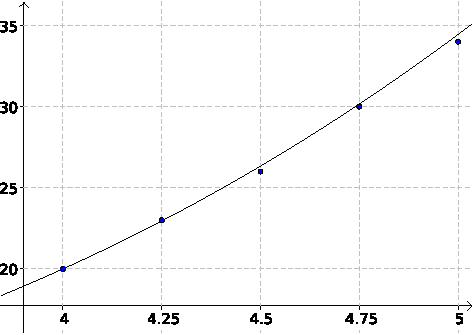
\includegraphics{figures/ode-pendulum14}
\par\end{center}

\noindent Dari grafik, satu-satunya titik pada hampiran yang tampak
terpisah dari grafik solusi eksak adalah titik $(5,34)$. Selisih
relatifnya pun hanya kecil. Lebih tepatnya, galat relatif di titik
tersebut adalah $\frac{|f(5)-34|}{|f(5)|}=\frac{9}{689}\approx0.013$.
Setiap komentar umum tentang akurasi suatu hampiran harus mempertimbangkan
kebutuhan dalam situasi tersebut. Dalam kasus ini, tidak ada konteks
yang menentukan apakah kita mengharapkan galat relatif $10$\%, $1$\%,
$.1\%$, atau yang lebih kecil, maupun apakah galat absolut lebih
penting. Tanpa konteks tersebut, kita cukup menggunakan representasi
visual, yang menunjukkan bahwa titik-titik hampiran sangat dekat dengan
grafik solusi eksak, lalu menyimpulkan bahwa hampiran tersebut merupakan
representasi yang baik dari solusi eksak.
\item [{\ref{exc:odePendulum-22}:}] Gaya yang bekerja pada balok diam
di bidang miring adalah gaya gravitasi, gesekan, dan gaya normal dari
permukaan tempat balok berada. Gaya gravitasi bekerja vertikal ke
bawah. Gesekan bekerja sejajar permukaan dan ke atas bidang miring
karena melawan gaya gravitasi yang menarik balok ke bawah bidang miring.
Gaya normal bekerja tegak lurus terhadap permukaan. Dengan merepresentasikan
balok sebagai persegi panjang dan setiap gaya sebagai vektor, diagram
benda bebas akan tampak kira-kira seperti ini:

\begin{center}
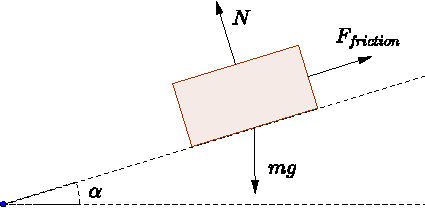
\includegraphics{figures/ode-pendulum07}
\par\end{center}

Perhatikan bahwa garis yang merepresentasikan permukaan BUKAN bagian
dari diagram benda bebas, sehingga digambar putus-putus. Garis tersebut
hanya menunjukkan arah gerak (yang mungkin terjadi).
\item [{\ref{exc:odePendulum-24}:}] Gaya yang bekerja pada sofa yang didorong
melintasi lantai datar adalah gaya gravitasi, gesekan, gaya normal
lantai, dan gaya terapan. Gaya gravitasi bekerja vertikal ke bawah.
Gesekan bekerja sejajar lantai dan melawan gaya terapan. Gaya normal
bekerja tegak lurus terhadap lantai. Gaya terapan bekerja dalam arah
yang tidak ditentukan dan tidak sejajar dengan lantai. Dengan merepresentasikan
sofa sebagai persegi panjang dan setiap gaya sebagai vektor, diagram
benda bebas akan tampak kira-kira seperti ini:

\begin{center}
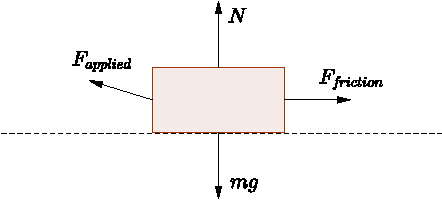
\includegraphics{figures/ode-pendulum15}
\par\end{center}

Perhatikan bahwa garis yang merepresentasikan lantai BUKAN bagian
dari diagram benda bebas, sehingga digambar putus-putus. Garis tersebut
hanya menunjukkan arah gerak.
\item [{\ref{exc:odePendulum-30}:}] Gaya yang bekerja pada penerjun payung---baik
parasutnya terbuka, tertutup, maupun sedang membuka---adalah gaya
gravitasi dan gaya hambat (hambatan udara). Gaya gravitasi bekerja
vertikal ke bawah dan gaya hambat bekerja vertikal ke atas. Dengan
merepresentasikan penerjun sebagai persegi panjang dan setiap gaya
sebagai vektor, diagram benda bebas akan tampak kira-kira seperti
ini:

\begin{center}
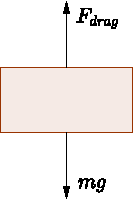
\includegraphics{figures/ode-pendulum11}
\par\end{center}
\item [{\ref{exc:odePendulum-34}c:}] (Lihat penyelesaian \ref{exc:odePendulum-22}
untuk diagram benda bebas) Karena balok tidak bergerak, gaya resultan
dalam setiap arah harus nol! Dengan demikian, persamaan geraknya adalah
$s(t)=0$. Selesai. Ini menjawab pertanyaan yang diajukan. 

Namun, ketika balok bergerak, perlu dipertimbangkan magnitudo gaya-gaya
yang bekerja dalam arah gerak, yaitu gesekan dan gravitasi. Sebagai
pembahasan, berikut cara menguraikan gaya-gaya tersebut. Gaya normal
bekerja tegak lurus terhadap gerak sehingga komponen tangensialnya
nol. Gesekan sebanding dengan gaya normal, dan secara konvensi kita
menggunakan $\mu$ sebagai konstanta proporsionalitas, sehingga magnitudo
gesekan adalah $\mu N$. Dengan menambahkan garis bantu yang tegak
lurus terhadap permukaan, terlihat bahwa komponen gravitasi dalam
arah tangensial adalah $mg\sin\alpha$.

\begin{center}
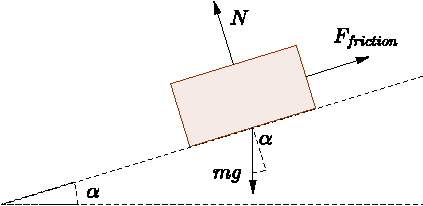
\includegraphics{figures/ode-pendulum16}
\par\end{center}

Dengan menetapkan arah positif ke bawah bidang miring, gaya yang bekerja
secara tangensial (sejajar) terhadap permukaan adalah $mg\sin\alpha-\mu N$.
Untuk melengkapi persamaan gerak, kita perlu menghitung $N$. Karena
balok tidak bergerak dalam arah normal, gaya resultan dalam arah tersebut
harus nol. Satu-satunya gaya yang bekerja dalam arah normal adalah
gaya normal itu sendiri dan salah satu komponen gravitasi. Oleh karena
itu, $N$ harus sama dengan magnitudo gaya gravitasi dalam arah normal.
Dengan kembali menggunakan garis bantu, komponen gravitasi dalam arah
normal adalah $mg\cos\alpha.$ Maka $N=mg\cos\alpha$. Dengan menyubstitusikan
bentuk ini ke gaya tangensial, diperoleh $mg\sin\alpha-\mu mg\cos\alpha$
yang bekerja secara tangensial terhadap permukaan. Menurut Hukum Kedua
Newton, gaya ini harus sama dengan $ma$, sehingga persamaan geraknya
adalah $m\ddot{s}=mg\sin\alpha-\mu mg\cos\alpha$, yang disederhanakan
menjadi 
\[
\ddot{s}=g(\sin\alpha-\mu\cos\alpha).
\]
Persamaan ini dapat digunakan untuk balok yang bergerak menuruni bidang
miring.
\item [{\ref{exc:odePendulum-34}f:}] (Lihat penyelesaian \ref{exc:odePendulum-24}
untuk diagram benda bebas) Gaya gravitasi dan gaya normal sama-sama
bekerja tegak lurus terhadap gerak, sehingga komponen tangensialnya
nol. Satu-satunya gaya yang bekerja (dengan komponen tak nol) dalam
arah gerak adalah gesekan dan gaya terapan. Gesekan sebanding dengan
gaya normal, dan secara konvensi kita menggunakan $\mu$ sebagai konstanta
proporsionalitas, sehingga magnitudo gesekan adalah $\mu N$. Dengan
menambahkan garis bantu yang sejajar permukaan, kita menandai sudut
gaya terapan dan melihat bahwa komponen gaya terapan dalam arah tangensial
adalah $F_{applied}\cos\beta$.

\begin{center}
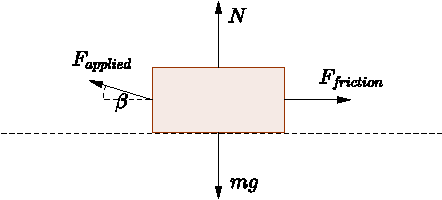
\includegraphics{figures/ode-pendulum17}
\par\end{center}

Dengan menetapkan arah positif ke kiri, gaya yang bekerja secara tangensial
(sejajar) terhadap permukaan adalah $F_{applied}\cos\beta-\mu N$.
Untuk melengkapi persamaan gerak, kita perlu menghitung $N$. Karena
balok tidak bergerak dalam arah normal, gaya resultan dalam arah normal
harus nol. Gaya yang bekerja dalam arah tersebut adalah $N$ itu sendiri,
gaya gravitasi, dan salah satu komponen gaya terapan. Oleh karena
itu, dalam arah normal harus berlaku $N+F_{applied}\sin\beta=mg$
atau $N=mg-F_{applied}\sin\beta$. Dengan menyubstitusikan bentuk
ini ke gaya tangensial, diperoleh $F_{applied}\cos\beta-\mu(mg-F_{applied}\sin\beta)$
yang bekerja secara tangensial terhadap permukaan. Menurut Hukum Kedua
Newton, gaya ini harus sama dengan $ma$, sehingga persamaan geraknya
adalah $m\ddot{s}=F_{applied}\cos\beta-\mu(mg-F_{applied}\sin\beta)$,
yang disederhanakan menjadi 
\[
\ddot{s}=\frac{F_{applied}}{m}(\cos\beta+\mu\sin\beta)-\mu g.
\]

\item [{\ref{exc:odePendulum-34}m:}] (Lihat penyelesaian \ref{exc:odePendulum-30}
untuk diagram benda bebas) Kedua gaya dalam diagram benda bebas bekerja
dalam arah vertikal, sehingga persamaan gerak dalam kasus ini sangat
sederhana. Trigonometri tidak diperlukan. $F=ma$ menjadi $F_{drag}-mg=m\ddot{s}$,
dengan menetapkan arah ke atas sebagai arah positif. Gaya hambat dianggap
sebanding dengan kelajuan tetapi berlawanan arah, sehingga $F_{drag}$
dapat diganti dengan $-c\dot{s}$ (untuk suatu konstanta positif $c$)
dan persamaan geraknya, secara lebih tepat, menjadi $-c\dot{s}-mg=m\ddot{s}$.
Dengan sedikit manipulasi aljabar, persamaan ini dapat ditulis ulang
sebagai
\[
\ddot{s}+\frac{c}{m}\dot{s}+g=0.
\]
\end{description}

\section*{Bagian \ref{sec:TaylorMethods}}
\begin{description}
\item [{\ref{exc:ode-taylor-6}:}] Dengan mengganti $t$ dalam metode Euler
(\ref{eq:EulersMethodConstantStepSize}) dengan $x$, metode Euler
yang diterapkan pada masalah ini berbentuk $y_{i+1}=y_{i}+h\cdot y'(x_{i},y_{i})$.
Karena kondisi awalnya adalah $y(1)=1$, kita mulai dengan $x_{0}=1$
dan $y_{0}=1$. Selanjutnya, 
\begin{eqnarray*}
y_{1} & = & y_{0}+0.5(3x_{0}-2y_{0})\\
 & = & 1+0.5(3(1)-2(1))\\
 & = & 1.5\\
x_{1} & = & x_{0}+h=1+0.5=1.5
\end{eqnarray*}
Sekarang $x_{0}$ dan $y_{0}$ tidak lagi diperlukan ketika kita menghitung
$x_{2}$ dan $y_{2}$:
\begin{eqnarray*}
y_{2} & = & y_{1}+0.5(3x_{1}-2y_{1})\\
 & = & 1.5+0.5(3(1.5)-2(1.5))\\
 & = & 2.25\\
x_{2} & = & x_{1}+h=1.5+0.5=2.0
\end{eqnarray*}
Oleh karena itu, diperoleh $y(2)\approx2.25$.
\item [{\ref{exc:ode-taylor-8}:}] Karena PDB tidak ditulis dalam bentuk
$y'=f(t,y)$, kita perlu menuliskannya kembali dalam bentuk tersebut
dengan menggunakan informasi yang diberikan dan menyelesaikannya untuk
$y'$:
\begin{eqnarray*}
\cos(x)y'+\sin(x)y & = & 2\cos^{3}(x)\sin(x)-1\\
\cos(x)y' & = & 2\cos^{3}(x)\sin(x)-1-\sin(x)y\\
y' & = & \frac{2\cos^{3}(x)\sin(x)-1-\sin(x)y}{\cos(x)}\\
 & = & 2\cos^{2}(x)\sin(x)-\sec(x)-y\tan(x)
\end{eqnarray*}
Jadi, diperoleh $f(x,y)=2\cos^{2}(x)\sin(x)-\sec(x)-y\tan(x)$. Sekarang,
dengan mengganti $t$ dalam metode Euler (\ref{eq:EulersMethodConstantStepSize})
dengan $x$, metode Euler yang diterapkan pada masalah ini berbentuk
$y_{i+1}=y_{i}+h\cdot y'(x_{i},y_{i})$. Karena kondisi awalnya adalah
$y(1)=0$, kita mulai dengan $x_{0}=1$ dan $y_{0}=0$. Selanjutnya,
\begin{eqnarray*}
y_{1} & = & y_{0}+0.5f(x_{0},y_{0})\\
 & = & 0+0.5f(1,0)\\
 & = & 0.5(2\cos^{2}(1)\sin(1)-\sec(1))\\
 & \approx & -0.67976011062352\\
x_{1} & = & x_{0}+h=1+0.5=1.5
\end{eqnarray*}
Sekarang $x_{0}$ dan $y_{0}$ tidak lagi diperlukan ketika kita menghitung
$x_{2}$ dan $y_{2}$:
\begin{eqnarray*}
y_{2} & = & y_{1}+0.5f(x_{1},y_{1})\\
 & \approx & -0.67976+0.5f(1.5,-0.67976)\\
 & \approx & -2.9503939532546\\
x_{2} & = & x_{1}+h=1.5+0.5=2.0
\end{eqnarray*}
Oleh karena itu, diperoleh $y(2)\approx-2.9503939532546$.
\item [{\ref{exc:ode-taylor-9}a:}] Untuk metode Taylor derajat 2, kita
memerlukan turunan kedua dari $y$. Satu-satunya informasi yang dapat
digunakan adalah PDB itu sendiri, $\frac{dy}{dx}=3x-2y$. Dengan diferensiasi
implisit,
\[
\frac{d^{2}y}{dx^{2}}=3-2\frac{dy}{dx}.
\]
Namun, bentuk ini belum memberikan $y''$ dalam $x$ dan $y$. Kita
harus menyubstitusikan $\frac{dy}{dx}$ dalam $x$ dan $y$. Namun,
itulah tepatnya yang diberikan oleh PDB! Dengan menyubstitusikan $\frac{dy}{dx}=3x-2y$
ke dalam bentuk untuk $\frac{d^{2}y}{dx^{2}}$ diperoleh
\begin{eqnarray*}
\frac{d^{2}y}{dx^{2}} & = & 3-2(3x-2y)\\
 & = & 3-6x+4y.
\end{eqnarray*}
Sekarang kita siap. Secara simbolis, metode Taylor derajat 2 adalah
\begin{eqnarray*}
y_{i+1} & = & y_{i}+h\cdot y'(x_{i},y_{i})+\frac{1}{2}h^{2}\cdot y''(x_{i},y_{i})\\
x_{i+1} & = & x_{i}+h
\end{eqnarray*}
Dimulai dari kondisi awal, $x_{0}=y_{0}=1$,
\begin{eqnarray*}
y_{1} & = & y_{0}+h\cdot y'(x_{0},y_{0})+\frac{1}{2}h^{2}\cdot y''(x_{0},y_{0})\\
 & = & 1+0.5(3\cdot1-2\cdot1)+\frac{1}{2}(0.5)^{2}\cdot(3-6\cdot1+4\cdot1)\\
 & = & 1.625\\
x_{1} & = & x_{0}+h=1+0.5=1.5
\end{eqnarray*}
Sekarang $x_{0}$ dan $y_{0}$ tidak lagi diperlukan ketika kita menghitung
$x_{2}$ dan $y_{2}$:
\begin{eqnarray*}
y_{2} & = & y_{1}+h\cdot y'(x_{1},y_{1})+\frac{1}{2}h^{2}\cdot y''(x_{1},y_{1})\\
 & = & 1.625+0.5(3\cdot1.5-2\cdot1.625)+\frac{1}{2}(0.5)^{2}\cdot(3-6\cdot1.5+4\cdot1.625)\\
 & = & 2.3125\\
x_{1} & = & x_{0}+h=1.5+0.5=2.0
\end{eqnarray*}
Oleh karena itu, diperoleh $y(2)=2.3125$.
\item [{\ref{exc:ode-taylor-9}d:}] Untuk metode Taylor derajat 2, kita
memerlukan turunan kedua dari $y$. Satu-satunya informasi yang dapat
digunakan adalah PDB itu sendiri (setelah diselesaikan untuk $\frac{dy}{dx}$:
$\frac{dy}{dx}=2\cos^{2}(x)\sin(x)-\sec(x)-y\tan(x)$. Dengan diferensiasi
implisit,
\[
\frac{d^{2}y}{dx^{2}}=-\tan(x)\cdot\frac{dy}{dx}-\sec(x)\tan(x)-4\cos(x)\sin^{2}(x)-y\sec^{2}(x)+2\cos^{3}(x).
\]
Namun, bentuk ini belum memberikan $y''$ dalam $x$ dan $y$. Kita
harus menyubstitusikan $\frac{dy}{dx}$ dalam $x$ dan $y$. Namun,
itulah tepatnya yang diberikan oleh PDB! Dengan menyubstitusikan $\frac{dy}{dx}=2\cos^{2}(x)\sin(x)-\sec(x)-y\tan(x)$
ke dalam bentuk untuk $\frac{d^{2}y}{dx^{2}}$ (dan menyederhanakannya
secara ekstensif!) diperoleh
\[
\frac{d^{2}y}{dx^{2}}=-y+8\cos^{3}(x)-6\cos(x)
\]
Sekarang kita siap. Secara simbolis, metode Taylor derajat 2 adalah
\begin{eqnarray*}
y_{i+1} & = & y_{i}+h\cdot y'(x_{i},y_{i})+\frac{1}{2}h^{2}\cdot y''(x_{i},y_{i})\\
x_{i+1} & = & x_{i}+h
\end{eqnarray*}
Dimulai dari kondisi awal, $x_{0}=1,\ y_{0}=0$,
\begin{eqnarray*}
y_{1} & = & y_{0}+h\cdot y'(x_{0},y_{0})+\frac{1}{2}h^{2}\cdot y''(x_{0},y_{0})\\
 & = & 0+0.5(2\cos^{2}(1)\sin(1)-\sec(1))\\
 &  & \quad+\frac{1}{2}(0.5)^{2}\cdot(8\cos^{3}(1)-6\cos(1))\\
 & \approx & -0.92725823477363\\
x_{1} & = & x_{0}+h=1+0.5=1.5
\end{eqnarray*}
Sekarang $x_{0}$ dan $y_{0}$ tidak lagi diperlukan ketika kita menghitung
$x_{2}$ dan $y_{2}$:
\begin{eqnarray*}
y_{2} & = & y_{1}+h\cdot y'(x_{1},y_{1})+\frac{1}{2}h^{2}\cdot y''(x_{1},y_{1})\\
 & \approx & -0.9272+0.5f(1.5,-0.9272)+\frac{1}{2}(0.5)^{2}\cdot y''(1.5,-0.9272)\\
 & \approx & -1.3896462555267\\
x_{1} & = & x_{0}+h=1.5+0.5=2.0
\end{eqnarray*}
Oleh karena itu, diperoleh $y(2)=-1.3896462555267$. Jika latihan
ini belum meyakinkan Anda bahwa metode Taylor dengan derajat lebih
tinggi dari 2 tidak terlalu praktis bagi pengguna, tunggulah sampai
Anda mencoba metode Taylor derajat 3 pada masalah ini.
\item [{\ref{exc:ode-taylor-10}a:}] Untuk metode Taylor derajat 3, kita
memerlukan turunan kedua serta turunan ketiga dari $y$. Satu-satunya
informasi yang dapat digunakan adalah PDB itu sendiri, $\frac{dy}{dx}=3x-2y$.
Dengan diferensiasi implisit,
\[
\frac{d^{2}y}{dx^{2}}=3-2\frac{dy}{dx}.
\]
Namun, bentuk ini belum memberikan $y''$ dalam $x$ dan $y$. Kita
harus menyubstitusikan $\frac{dy}{dx}$ dalam $x$ dan $y$. Namun,
itulah tepatnya yang diberikan oleh PDB! Dengan menyubstitusikan $\frac{dy}{dx}=3x-2y$
ke dalam bentuk untuk $\frac{d^{2}y}{dx^{2}}$ diperoleh
\begin{eqnarray*}
\frac{d^{2}y}{dx^{2}} & = & 3-2(3x-2y)\\
 & = & 3-6x+4y.
\end{eqnarray*}
Dengan mendiferensiasikan secara implisit persamaan untuk $\frac{d^{2}y}{dx^{2}}$
diperoleh
\begin{eqnarray*}
\frac{d^{3}y}{dx^{3}} & = & -6+4\cdot\frac{dy}{dx}\\
 & = & -6+4(3x-2y)\\
 & = & 12x-8y-6.
\end{eqnarray*}
Sekarang kita siap. Secara simbolis, metode Taylor derajat 3 adalah
\begin{eqnarray*}
y_{i+1} & = & y_{i}+h\cdot y'(x_{i},y_{i})+\frac{1}{2}h^{2}\cdot y''(x_{i},y_{i})+\frac{1}{6}h^{3}\cdot y'''(x_{i},y_{i})\\
x_{i+1} & = & x_{i}+h
\end{eqnarray*}
Dimulai dari kondisi awal, $x_{0}=y_{0}=1$,
\begin{eqnarray*}
y_{1} & = & y_{0}+h\cdot y'(x_{0},y_{0})+\frac{1}{2}h^{2}\cdot y''(x_{0},y_{0})+\frac{1}{6}h^{3}\cdot y'''(x_{0},y_{0})\\
 & = & 1+0.5(3\cdot1-2\cdot1)+\frac{1}{2}(0.5)^{2}\cdot(3-6\cdot1+4\cdot1)\\
 &  & \qquad+\frac{1}{6}(0.5)^{3}(12\cdot1-8\cdot1-6)\\
 & \approx & 1.5833333333333\\
x_{1} & = & x_{0}+h=1+0.5=1.5
\end{eqnarray*}
Sekarang $x_{0}$ dan $y_{0}$ tidak lagi diperlukan ketika kita menghitung
$x_{2}$ dan $y_{2}$:
\begin{eqnarray*}
y_{2} & = & y_{1}+h\cdot y'(x_{1},y_{1})+\frac{1}{2}h^{2}\cdot y''(x_{1},y_{1})+\frac{1}{6}h^{3}\cdot y'''(x_{1},y_{1})\\
 & \approx & 1.583+0.5(3\cdot1.5-2\cdot1.583)+\frac{1}{2}(0.5)^{2}\cdot(3-6\cdot1.5+4\cdot1.583)\\
 &  & \qquad+\frac{1}{6}(0.5)^{3}(12\cdot1.5-8\cdot1.583-6)\\
 & \approx & 2.2777777777777\\
x_{1} & = & x_{0}+h=1.5+0.5=2.0
\end{eqnarray*}
Oleh karena itu, diperoleh $y(2)=2.2777777777777$.
\item [{\ref{exc:ode-taylor-10}d:}] Untuk metode Taylor derajat 3, kita
memerlukan turunan kedua serta turunan ketiga dari $y$. Satu-satunya
informasi yang dapat digunakan adalah PDB itu sendiri (setelah diselesaikan
untuk $\frac{dy}{dx}$: $\frac{dy}{dx}=2\cos^{2}(x)\sin(x)-\sec(x)-y\tan(x)$.
Dengan diferensiasi implisit,
\[
\frac{d^{2}y}{dx^{2}}=-\tan(x)\cdot\frac{dy}{dx}-\sec(x)\tan(x)-4\cos(x)\sin^{2}(x)-y\sec^{2}(x)+2\cos^{3}(x).
\]
Namun, bentuk ini belum memberikan $y''$ dalam $x$ dan $y$. Kita
harus menyubstitusikan $\frac{dy}{dx}$ dalam $x$ dan $y$. Namun,
itulah tepatnya yang diberikan oleh PDB! Dengan menyubstitusikan $\frac{dy}{dx}=2\cos^{2}(x)\sin(x)-\sec(x)-y\tan(x)$
ke dalam bentuk untuk $\frac{d^{2}y}{dx^{2}}$ (dan menyederhanakannya
secara ekstensif!) diperoleh
\[
\frac{d^{2}y}{dx^{2}}=-y+8\cos^{3}(x)-6\cos(x)
\]
Dengan mendiferensiasikan secara implisit persamaan untuk $\frac{d^{2}y}{dx^{2}}$
diperoleh
\begin{eqnarray*}
\frac{d^{3}y}{dx^{3}} & = & -\frac{dy}{dx}-24\cos^{2}(x)\sin(x)+6\sin(x)\\
 & = & y\tan(x)+(6-26\cos^{2}(x))\sin(x)+\sec(x)
\end{eqnarray*}
Sekarang kita siap. Secara simbolis, metode Taylor derajat 3 adalah
\begin{eqnarray*}
y_{i+1} & = & y_{i}+h\cdot y'(x_{i},y_{i})+\frac{1}{2}h^{2}\cdot y''(x_{i},y_{i})+\frac{1}{6}h^{3}\cdot y'''(x_{i},y_{i})\\
x_{i+1} & = & x_{i}+h
\end{eqnarray*}
Dimulai dari kondisi awal, $x_{0}=1,\ y_{0}=0$,
\begin{eqnarray*}
y_{1} & = & y_{0}+h\cdot y'(x_{0},y_{0})+\frac{1}{2}h^{2}\cdot y''(x_{0},y_{0})+\frac{1}{6}h^{3}\cdot y'''(x_{0},y_{0})\\
 & = & 0+0.5(2\cos^{2}(1)\sin(1)-\sec(1))\\
 &  & \quad+\frac{1}{2}(0.5)^{2}\cdot(8\cos^{3}(1)-6\cos(1))\\
 &  & \quad+\frac{1}{6}(0.5)^{3}\cdot(\sec(1)+(6-26\cos^{2}(1))\sin(1))\\
 & \approx & -0.91657489783846\\
x_{1} & = & x_{0}+h=1+0.5=1.5
\end{eqnarray*}
Sekarang $x_{0}$ dan $y_{0}$ tidak lagi diperlukan ketika kita menghitung
$x_{2}$ dan $y_{2}$:
\begin{eqnarray*}
y_{2} & = & y_{1}+h\cdot y'(x_{1},y_{1})+\frac{1}{2}h^{2}\cdot y''(x_{1},y_{1})+\frac{1}{6}h^{3}\cdot y'''(x_{1},y_{1})\\
 & \approx & -0.9166+0.5f(1.5,-0.9166)+\frac{1}{2}(0.5)^{2}\cdot y''(1.5,-0.9166)\\
 &  & \qquad+\frac{1}{6}(0.5)^{3}\cdot y'''(1.5,-0.9166)\\
 & \approx & -1.3083937870918\\
x_{1} & = & x_{0}+h=1.5+0.5=2.0
\end{eqnarray*}
Oleh karena itu, diperoleh $y(2)=-1.3083937870918$. Jika latihan
ini belum meyakinkan Anda bahwa metode Taylor dengan derajat lebih
tinggi dari 2 tidak terlalu praktis bagi pengguna, tidak ada lagi
yang dapat meyakinkan Anda!
\item [{\ref{exc:ode-taylor-2}:}] Ingatlah untuk mendokumentasikan kode
Anda! Dokumentasi suatu fungsi hampir selalu sebaiknya ditulis sebelum
fungsi itu sendiri. Menuliskan dengan tepat masukan dan keluaran yang
dimaksudkan bagi fungsi tersebut akan membantu mengarahkan penulisannya.
Dari kode semu metode Euler, masukannya adalah persamaan diferensial
$\dot{y}=f(t,y)$; kondisi awal $y(t_{0})=y_{0}$; bilangan $t_{0}$
dan $t_{1}$; serta jumlah langkah $N$. Komentar yang wajar pada
awal fungsi akan mencantumkan semua masukan dan keluaran tersebut,
sekaligus mendokumentasikan siapa yang menulisnya, kapan, dan untuk
tujuan apa:

\begin{lyxcode}
\%\%\%\%\%\%\%\%\%\%\%\%\%\%\%\%\%\%\%\%\%\%\%\%\%\%\%\%\%\%\%\%\%\%\%\%\%\%\%\%\%\%\%\%\%\%\%\%\%\%\%\%\%\%\%\%\%\%\%\%\%\%\%\%\%\%

\%~Written~by~Leon~Brin~~~~~~~~~~~~~~~~~~~~~~~~~~~29~January~2012~\%

\%~Purpose:~This~function~implements~Euler's~method~where~the~~~~~\%

\%~~~~~~~~step~size~is~calculated~and~held~constant.~~~~~~~~~~~~~~\%

\%~INPUT:~function~f(x,y);~interval~{[}a,b{]};~y(a);~steps~n~~~~~~~~~~\%

\%~OUTPUT:~approximation~(x(i),y(i))~of~the~solution~of~y'=f(x,y)~\%

\%\%\%\%\%\%\%\%\%\%\%\%\%\%\%\%\%\%\%\%\%\%\%\%\%\%\%\%\%\%\%\%\%\%\%\%\%\%\%\%\%\%\%\%\%\%\%\%\%\%\%\%\%\%\%\%\%\%\%\%\%\%\%\%\%\%
\end{lyxcode}
Deklarasi fungsi harus memuat kelima masukan sebagai argumen dan keluarannya
sebagai nilai balik. Bentuk seperti \texttt{function {[}y,x{]} = eulerode(f,a,ya,b,n)}
dapat digunakan, dengan \texttt{ya} tentu saja merupakan masukan $y(a)$.
Bagian fungsi selanjutnya seharusnya mengikuti kode semu hampir secara
harfiah. Saya menggunakan $x$ sebagai pengganti $t$ untuk variabel
bebas.\index{metode Euler!kode} \texttt{eulerode.m} dapat diunduh
di \href{http://lqbrin.github.io/tea-time-numerical/ancillaries.html}{situs pendamping}.\label{code:euler}
\begin{lyxcode}
\%\%\%\%\%\%\%\%\%\%\%\%\%\%\%\%\%\%\%\%\%\%\%\%\%\%\%\%\%\%\%\%\%\%\%\%\%\%\%\%\%\%\%\%\%\%\%\%\%\%\%\%\%\%\%\%\%\%\%\%\%\%\%\%\%\%

\%~Written~by~Leon~Brin~~~~~~~~~~~~~~~~~~~~~~~~~~~29~January~2012~\%

\%~Purpose:~This~function~implements~Euler's~method~where~the~~~~~\%

\%~~~~~~~~step~size~is~calculated~and~held~constant.~~~~~~~~~~~~~~\%

\%~INPUT:~function~f(x,y);~interval~{[}a,b{]};~y(a);~steps~n~~~~~~~~~~\%

\%~OUTPUT:~approximation~(x(i),y(i))~of~the~solution~of~y'=f(x,y)~\%

\%\%\%\%\%\%\%\%\%\%\%\%\%\%\%\%\%\%\%\%\%\%\%\%\%\%\%\%\%\%\%\%\%\%\%\%\%\%\%\%\%\%\%\%\%\%\%\%\%\%\%\%\%\%\%\%\%\%\%\%\%\%\%\%\%\%

function~{[}y,x{]}~=~eulerode(f,a,ya,b,n)

~~i~=~1;

~~x(i)~=~a;

~~y(i)~=~ya;

~~h~=~(b-a)/n;

~~while~(i<=n)

~~~~y(i+1)~=~y(i)~+~h{*}f(x(i),y(i));

~~~~x(i+1)~=~a~+~(b-a){*}i/n;

~~~~i~=~i+1;

~~end\%while

end\%function~
\end{lyxcode}
\item [{\ref{exc:ode-taylor-13}c:}] Persamaan geraknya adalah $\ddot{s}=g(\sin\alpha-\mu\cos\alpha)$.
Persamaan ini merupakan PDB orde kedua dengan variabel terikat $s$
dan variabel bebas $t$. Besaran $g$, $\alpha$, dan $\mu$ yang
muncul dalam persamaan merupakan konstanta. Misalkan $u=\dot{s}$
sehingga $\dot{u}=\ddot{s}=g(\sin\alpha-\mu\cos\alpha)$, dan sistem
orde pertamanya menjadi
\begin{eqnarray*}
\dot{u} & = & g(\sin\alpha-\mu\cos\alpha)\\
\dot{s} & = & u
\end{eqnarray*}
\item [{\ref{exc:ode-taylor-13}f:}] Persamaan geraknya adalah $\ddot{s}=\frac{F_{applied}}{m}(\cos\beta+\mu\sin\beta)-\mu g$.
Persamaan ini merupakan PDB orde kedua dengan variabel terikat $s$
dan variabel bebas $t$. Besaran $\beta$, $m$, $F_{applied}$, dan
$\mu$ yang muncul dalam persamaan merupakan konstanta. Misalkan $u=\dot{s}$
sehingga $\dot{u}=\ddot{s}=\frac{F_{applied}}{m}(\cos\beta+\mu\sin\beta)-\mu g$,
dan sistem orde pertamanya menjadi
\begin{eqnarray*}
\dot{u} & = & \frac{F_{applied}}{m}(\cos\beta+\mu\sin\beta)-\mu g\\
\dot{s} & = & u
\end{eqnarray*}
\item [{\ref{exc:ode-taylor-13}m:}] Persamaan geraknya adalah $\ddot{s}+\frac{c}{m}\dot{s}+g=0$.
Persamaan ini merupakan PDB orde kedua dengan variabel terikat $s$
dan variabel bebas $t$. Besaran $c$, $m$, dan $g$ yang muncul
dalam persamaan merupakan konstanta. Misalkan $u=\dot{s}$ sehingga
$\dot{u}=\ddot{s}=-\frac{c}{m}\dot{s}-g$, dan sistem orde pertamanya
menjadi
\begin{eqnarray*}
\dot{u} & = & -\frac{c}{m}u-g\\
\dot{s} & = & u
\end{eqnarray*}
\item [{\ref{exc:ode-taylor-21}c:}] Sistem yang kita selesaikan adalah
\begin{eqnarray*}
\dot{u} & = & g(\sin\alpha-\mu\cos\alpha)\\
\dot{s} & = & u
\end{eqnarray*}
dengan kondisi awal $s(0)=0$, $\dot{s}(0)=0$ dan nilai parameter
$g=32.2$ ft/s$^{2}$, $\mu=.21$, $\alpha=.25$ rad. Konversi satuan
tidak diperlukan. Kita memasukkan nilai parameter ke dalam sistem
untuk memperoleh masalah nilai awal
\begin{eqnarray*}
\dot{u} & = & 1.41462169238826\\
\dot{s} & = & u\\
u_{0} & = & \dot{s}(0)=0\\
s_{0} & = & s(0)=0
\end{eqnarray*}
Menerapkan metode Euler pada sistem ini berarti mengiterasikan
\begin{eqnarray*}
u_{n+1} & = & u_{n}+h\dot{u}(u_{n},s_{n})=u_{n}+0.25(1.41462169238826)\\
s_{n+1} & = & s_{n}+h\dot{s}(u_{n},s_{n})=s_{n}+0.25u_{n}\\
t_{n+1} & = & t_{n}+h
\end{eqnarray*}
Khususnya,
\begin{eqnarray*}
u_{1} & = & u_{0}+0.25\dot{u}(u_{0},s_{0})\\
 & = & 0+0.25(1.41462169238826)\approx0.353655423097065\\
s_{1} & = & s_{0}+0.25u_{0}\\
 & = & 0+0.25(0)=0\\
t_{1} & = & t_{0}+0.25=.25
\end{eqnarray*}
dan
\begin{eqnarray*}
u_{2} & = & u_{1}+0.25\dot{u}(u_{1},s_{1})\\
 & \approx & 0.3536+0.25(1.414)\approx0.7073108461941298\\
s_{2} & = & s_{1}+0.25u_{1}\\
 & \approx & 0+0.25(0.3536)\approx0.08841385577426622\\
t_{1} & = & t_{0}+0.25=.5
\end{eqnarray*}
Oleh karena itu, $s(0.5)\approx0.08841385577426622$.
\item [{\ref{exc:ode-taylor-21}f:}] Sistem yang kita selesaikan adalah
\begin{eqnarray*}
\dot{u} & = & \frac{F_{applied}}{m}(\cos\beta+\mu\sin\beta)-\mu g\\
\dot{s} & = & u
\end{eqnarray*}
dengan kondisi awal $s(0)=0$, $\dot{s}(0)=.03$ dan nilai parameter
$g=9.81$ m/s$^{2}$, $\mu=.15$, $\beta=\frac{\pi}{10}$ rad, $m=35$
kg, dan $F_{applied}=75$ N. Konversi satuan tidak diperlukan. Kita
memasukkan nilai parameter ke dalam sistem untuk memperoleh masalah
nilai awal
\begin{eqnarray*}
\dot{u} & = & \frac{75}{35}\left(\cos\left(\frac{\pi}{10}\right)+.15\sin\left(\frac{\pi}{10}\right)\right)-.15(9.81)\approx0.6658051402529905\\
\dot{s} & = & u\\
u_{0} & = & \dot{s}(0)=.03\\
s_{0} & = & s(0)=0
\end{eqnarray*}
Menerapkan metode Euler pada sistem ini berarti mengiterasikan
\begin{eqnarray*}
u_{n+1} & = & u_{n}+h\dot{u}(u_{n},s_{n})=u_{n}+0.25(0.6658051402529905)\\
s_{n+1} & = & s_{n}+h\dot{s}(u_{n},s_{n})=s_{n}+0.25u_{n}\\
t_{n+1} & = & t_{n}+h
\end{eqnarray*}
Khususnya,
\begin{eqnarray*}
u_{1} & = & u_{0}+0.25\dot{u}(u_{0},s_{0})\\
 & = & .03+0.25(0.6658051402529905)\approx0.1964512850632476\\
s_{1} & = & s_{0}+0.25u_{0}\\
 & = & 0+0.25(.03)=0.0075\\
t_{1} & = & t_{0}+0.25=.25
\end{eqnarray*}
dan
\begin{eqnarray*}
u_{2} & = & u_{1}+0.25\dot{u}(u_{1},s_{1})\\
 & \approx & 0.1964+0.25(0.6658)\approx0.3629025701264953\\
s_{2} & = & s_{1}+0.25u_{1}\\
 & \approx & 0.0075+0.25(0.1964)\approx0.05661282126581191\\
t_{1} & = & t_{0}+0.25=.5
\end{eqnarray*}
Oleh karena itu, $s(0.5)\approx0.05661282126581191$.
\item [{\ref{exc:ode-taylor-21}m:}] Sistem yang kita selesaikan adalah
\begin{eqnarray*}
\dot{u} & = & -\frac{c}{m}u-g\\
\dot{s} & = & u
\end{eqnarray*}
dengan kondisi awal $s(0)=2000$, $\dot{s}(0)=-55$ dan nilai parameter
$g=9.81$ m/s$^{2}$, $c=26$, dan $m=70$ kg. Konversi satuan tidak
diperlukan. Kita memasukkan nilai parameter ke dalam sistem untuk
memperoleh masalah nilai awal
\begin{eqnarray*}
\dot{u} & = & \frac{26}{70}u-9.81=-\frac{13}{35}u-9.81\\
\dot{s} & = & u\\
u_{0} & = & \dot{s}(0)=-55\\
s_{0} & = & s(0)=2000
\end{eqnarray*}
Menerapkan metode Euler pada sistem ini berarti mengiterasikan
\begin{eqnarray*}
u_{n+1} & = & u_{n}+h\dot{u}(u_{n},s_{n})=u_{n}+0.25\left(-\frac{13}{35}u_{n}-9.81\right)\\
s_{n+1} & = & s_{n}+h\dot{s}(u_{n},s_{n})=s_{n}+0.25u_{n}\\
t_{n+1} & = & t_{n}+h
\end{eqnarray*}
Khususnya,
\begin{eqnarray*}
u_{1} & = & u_{0}+0.25\dot{u}(u_{0},s_{0})\\
 & = & -55+0.25\left(-\frac{13}{35}(-55)-9.81\right)\approx-52.34535714285715\\
s_{1} & = & s_{0}+0.25u_{0}\\
 & = & 2000+0.25(-55)=1986.25\\
t_{1} & = & t_{0}+0.25=.25
\end{eqnarray*}
dan
\begin{eqnarray*}
u_{2} & = & u_{1}+0.25\dot{u}(u_{1},s_{1})\\
 & \approx & -52.34+0.25\left(-\frac{13}{35}(-52.34)-9.81\right)\approx-49.9372168367347\\
s_{2} & = & s_{1}+0.25u_{1}\\
 & \approx & 1986.25+0.25(-52.34)\approx1973.163660714286\\
t_{1} & = & t_{0}+0.25=.5
\end{eqnarray*}
Oleh karena itu, $s(0.5)\approx1973.163660714286$.
\item [{\ref{exc:ode-taylor-14}:}] Sejumlah teknik penyelesaian persamaan
diferensial mengharuskan kita memiliki gambaran tentang bentuk solusi
sebelum mengetahui solusi tersebut secara tepat. Selanjutnya, kita
mengambil ``tebakan kasar'' dan menyempurnakannya dengan memaksanya
memenuhi persamaan diferensial yang diberikan. Metode koefisien tak
tentu merupakan contoh teknik semacam ini. Kita mengetahui bahwa solusi
merupakan kombinasi linear fungsi-fungsi tertentu, tetapi belum mengetahui
koefisien yang tepat. Untuk mencari koefisien tersebut, kita menyubstitusikan
solusi dengan koefisien yang belum diketahui (tak tentu) ke dalam
persamaan diferensial dan mencocokkan koefisien suku-suku sejenis.
Proses ini menghasilkan sistem persamaan linear yang harus diselesaikan
untuk mencari peubah-peubah tak diketahui. Dalam contoh ini, diberikan
bahwa $y(x)=Ax^{2}+Bx+C$ merupakan solusi dari $y''+5y'-8y=3x^{2}$,
dan kita perlu menentukan nilai $A$, $B$, dan $C$. Kita akan mencari
$y'$ dan $y''$ lalu menyubstitusikannya ke dalam PDB:
\begin{eqnarray*}
y'(x) & = & 2Ax+B\\
y''(x) & = & 2A
\end{eqnarray*}
Oleh karena itu,
\[
y''+5y'-8y=2A+5(2Ax+B)-8(Ax^{2}+Bx+C).
\]
Jadi, agar diperoleh solusi PDB, harus berlaku 
\[
2A+5(2Ax+B)-8(Ax^{2}+Bx+C)=3x^{2}
\]
Jika disederhanakan, bentuknya adalah
\[
-8Ax^{2}+(10A-8B)x+(2A+5B-8C)=3x^{2}.
\]
Dengan mencocokkan koefisien suku sejenis pada ruas kiri dan kanan,
diperoleh
\begin{eqnarray*}
-8A & = & 3\\
10A-8B & = & 0\\
2A+5B-8C & = & 0.
\end{eqnarray*}
Solusi sistem ini adalah $A=-\frac{3}{8}$, $B=-\frac{15}{32}$, $C=-\frac{99}{256}$.
Dengan demikian, solusi PDB adalah $y(x)=-\frac{3}{8}x^{2}-\frac{15}{32}x-\frac{99}{256}$.
\item [{\ref{exc:ode-taylor-18}:}] Sejumlah teknik penyelesaian persamaan
diferensial mengharuskan kita memiliki gambaran tentang bentuk solusi
sebelum mengetahui solusi tersebut secara tepat. Selanjutnya, kita
mengambil ``tebakan kasar'' dan menyempurnakannya dengan memaksanya
memenuhi persamaan diferensial yang diberikan. Metode koefisien tak
tentu merupakan contoh teknik semacam ini. Kita mengetahui bahwa solusi
merupakan kombinasi linear fungsi-fungsi tertentu, tetapi belum mengetahui
koefisien yang tepat. Untuk mencari koefisien tersebut, kita menyubstitusikan
solusi dengan koefisien yang belum diketahui (tak tentu) ke dalam
persamaan diferensial dan mencocokkan koefisien suku-suku sejenis.
Proses ini menghasilkan sistem persamaan linear yang harus diselesaikan
untuk mencari peubah-peubah tak diketahui. Dalam contoh ini, diberikan
bahwa $\theta(t)=At\cos t+Bt\sin t+C\cos t+D\sin t$ merupakan solusi
dari $\ddot{\theta}+\frac{1}{10}\dot{\theta}+\theta=t\cos t$, dan
kita perlu menentukan nilai $A$, $B$, $C$, dan $D$. Kita akan
mencari $\dot{\theta}$ dan $\ddot{\theta}$ lalu menyubstitusikannya
ke dalam PDB:
\begin{eqnarray*}
\dot{\theta(t)} & = & (D+A)\cos(t)+(B-C)\sin(t)+Bt\cos(t)-At\sin(t)\\
\ddot{\theta}(t) & = & (2B-C)\cos(t)+(-D-2A)\sin(t)-At\cos(t)-Bt\sin(t)
\end{eqnarray*}
Oleh karena itu,
\begin{eqnarray*}
\ddot{\theta}+\frac{1}{10}\dot{\theta}+\theta & = & (2B-C)\cos(t)+(-D-2A)\sin(t)-At\cos(t)-Bt\sin(t)\\
 &  & \quad+\frac{1}{10}\left((D+A)\cos(t)+(B-C)\sin(t)+Bt\cos(t)-At\sin(t)\right)\\
 &  & \quad+At\cos t+Bt\sin t+C\cos t+D\sin t
\end{eqnarray*}
Jika disederhanakan, bentuknya adalah
\begin{eqnarray*}
\ddot{\theta}+\frac{1}{10}\dot{\theta}+\theta & = & \left(\frac{1}{10}D+2B+\frac{1}{10}A\right)\cos(t)\\
 &  & +\left(B-C-2A\right)\sin(t)\\
 &  & +\frac{1}{10}Bt\cos(t)\\
 &  & -\frac{1}{10}At\sin(t)
\end{eqnarray*}
Jadi, agar diperoleh solusi PDB, harus berlaku 
\begin{eqnarray*}
\left(\frac{1}{10}D+2B+\frac{1}{10}A\right)\cos(t)\\
+\left(B-C-2A\right)\sin(t)\\
+\frac{1}{10}Bt\cos(t)\\
-\frac{1}{10}At\sin(t) & = & t\cos t
\end{eqnarray*}
Dengan mencocokkan koefisien suku sejenis pada ruas kiri dan kanan,
diperoleh
\begin{eqnarray*}
\frac{1}{10}D+2B+\frac{1}{10}A & = & 0\\
B-C-2A & = & 0\\
\frac{1}{10}B & = & 1\\
-\frac{1}{10}A & = & 0
\end{eqnarray*}
Solusi sistem ini adalah $A=0$, $B=10$, $C=10$, $D=-200$. Dengan
demikian, solusi PDB adalah $\theta(t)=10t\sin t-200\sin t+10\cos t$.
\end{description}

\section*{Bagian \ref{sec:Runge-Kutta-Methods}}
\begin{description}
\item [{\ref{exc:ode-rungeKutta-1}:}] Setiap pemecah PDB memiliki bentuk
\[
y_{i+1}=y_{i}+h(\mbox{rata-rata berbobot dari evaluasi }f).
\]
Rumus integrasilah yang memberi kita rata-rata berbobot. Dalam kasus
ini, rumus 
\[
\frac{h}{4}\left(f(x_{0})+3f\left(x_{0}+\frac{2}{3}h\right)\right)
\]
 meminta kita merata-ratakan $f(x_{0})$, nilai $f$ pada simpul pertama,
dengan $f(x_{0}+\frac{2}{3}h)$ dalam rasio $1:3$. Artinya, kita
menjumlahkan satu $f(x_{0})$ dengan tiga $f(x_{0}+\frac{2}{3}h)$
lalu membaginya dengan 4. Sayangnya, kita menggunakan $f$ di sini
dalam dua konteks yang berbeda. Variabel $f$ dalam pemecah PDB tidak
sama dengan $f$ yang digunakan dalam menurunkan rumus integrasi.
Variabel $f$ dari rumus integrasi merupakan fungsi satu variabel,
$x$. Variabel $f$ yang kita perlukan dalam pemecah PDB merupakan
fungsi dua variabel, $t$ dan $y$. Meskipun demikian, keduanya berperan
sama. Keduanya menyimpan nilai fungsi yang kita integralkan. Jika
kita perlu menjumlahkan satu $f(x_{0})$ dengan tiga $f(x_{0}+\frac{2}{3}h)$
dalam rumus integrasi, kita perlu menjumlahkan satu $f(t_{i},y_{i})$
dengan tiga $f(t_{i+2/3},y_{i+2/3})$ dalam pemecah PDB. Secara umum,
$f(x_{0}+\alpha h)$ dalam rumus integrasi berpadanan dengan $f(t_{i+\alpha},y_{i+\alpha})$
dalam pemecah PDB selama rumus integrasi ditulis untuk selang dengan
panjang $h$.

Setiap pemecah PDB dimulai dengan $k_{1}=f(t_{i},y_{i})$ dengan $(t_{i},y_{i})$
sebagai titik terakhir yang dihampiri. Setiap nilai berikutnya dalam
pemecah PDB diperoleh dengan menggunakan metode Euler dengan kondisi
awal (titik awal) $(t_{i},y_{i})$. Untuk rumus integrasi khusus ini,
hanya ada satu simpul selain $x_{0}$, sehingga kita hanya memerlukan
satu tahap lagi. Kita menghampiri $y_{i+2/3}$ dengan $y_{i}+\frac{2h}{3}k_{1}$
(metode Euler menggunakan titik awal $(t_{i},y_{i})$ dan gradien
hampiran $k_{1}$). Dengan demikian, $k_{2}=f(t_{i}+\frac{2h}{3},y_{i}+\frac{2h}{3}k_{1})$.
Langkah terakhir ialah menghitung rata-rata berbobot. Seperti dibahas,
kita perlu menjumlahkan satu $k_{1}$ dengan tiga $k_{2}$ lalu membaginya
dengan 4. Singkatnya, pemecah PDB yang disarankan oleh rumus integrasi
ini adalah
\begin{eqnarray*}
k_{1} & = & f(t_{i},y_{i})\\
k_{2} & = & f\left(t_{i}+\frac{2h}{3},y_{i}+\frac{2h}{3}k_{1}\right)\\
y_{i+1} & = & y_{i}+\frac{h}{4}\left[k_{1}+3k_{2}\right].
\end{eqnarray*}

\item [{\ref{exc:ode-rungeKutta-5}:}] Setiap pemecah PDB memiliki bentuk
\[
y_{i+1}=y_{i}+h(\mbox{rata-rata berbobot dari evaluasi }f).
\]
Rumus integrasilah yang memberi kita rata-rata berbobot. Dalam kasus
ini, rumus 
\[
\frac{h}{4}\left(3f\left(x_{0}+\frac{1}{3}h\right)+f(x_{0}+h)\right)
\]
 meminta kita merata-ratakan $f(x_{0}+\frac{1}{3}h)$, nilai $f$
pada simpul pertama, dengan $f(x_{0}+h)$ dalam rasio $3:1$. Artinya,
kita menjumlahkan tiga $f(x_{0}+\frac{1}{3}h)$ dengan satu $f(x_{0}+h)$
lalu membaginya dengan 4. Sayangnya, kita menggunakan $f$ di sini
dalam dua konteks yang berbeda. Variabel $f$ dalam pemecah PDB tidak
sama dengan $f$ yang digunakan dalam menurunkan rumus integrasi.
Variabel $f$ dari rumus integrasi merupakan fungsi satu variabel,
$x$. Variabel $f$ yang kita perlukan dalam pemecah PDB merupakan
fungsi dua variabel, $t$ dan $y$. Meskipun demikian, keduanya berperan
sama. Keduanya menyimpan nilai fungsi yang kita integralkan. Jika
kita perlu menjumlahkan tiga $f(x_{0}+\frac{1}{3}h)$ dengan satu
$f(x_{0}+h)$ dalam rumus integrasi, kita perlu menjumlahkan tiga
$f(t_{i+1/3},y_{i+1/3})$ dengan satu $f(t_{i+1},y_{i+1})$ dalam
pemecah PDB. Secara umum, $f(x_{0}+\alpha h)$ dalam rumus integrasi
berpadanan dengan $f(t_{i+\alpha},y_{i+\alpha})$ dalam pemecah PDB
selama rumus integrasi ditulis untuk selang dengan panjang $h$. 

Setiap pemecah PDB dimulai dengan $k_{1}=f(t_{i},y_{i})$ dengan $(t_{i},y_{i})$
sebagai titik terakhir yang dihampiri. Setiap nilai berikutnya dalam
pemecah PDB diperoleh dengan menggunakan metode Euler dengan kondisi
awal (titik awal) $(t_{i},y_{i})$. Untuk rumus integrasi khusus ini,
terdapat dua simpul selain $x_{0}$, sehingga kita memerlukan dua
tahap lagi. Kita menghampiri $y_{i+1/3}$ dengan $y_{i}+\frac{h}{3}k_{1}$
(metode Euler menggunakan titik awal $(t_{i},y_{i})$ dan gradien
hampiran $k_{1}$). Dengan demikian, $k_{2}=f(t_{i}+\frac{h}{3},y_{i}+\frac{h}{3}k_{1})$.
Selanjutnya, kita menghampiri $y_{i+1}$ dengan $y_{i}+hk_{2}$ (metode
Euler menggunakan titik awal $(t_{i},y_{i})$ dan gradien hampiran
$k_{2}$). Langkah terakhir ialah menghitung rata-rata berbobot. Seperti
dibahas, kita perlu menjumlahkan tiga $k_{2}$ dengan satu $k_{3}$
lalu membaginya dengan 4. Singkatnya, pemecah PDB yang disarankan
oleh rumus integrasi ini adalah
\begin{eqnarray*}
k_{1} & = & f(t_{i},y_{i})\\
k_{2} & = & f\left(t_{i}+\frac{h}{3},y_{i}+\frac{h}{3}k_{1}\right)\\
k_{3} & = & f\left(t_{i}+h,y_{i}+hk_{2}\right)\\
y_{i+1} & = & y_{i}+\frac{h}{4}\left[3k_{2}+k_{3}\right].
\end{eqnarray*}

\item [{\ref{exc:ode-rungeKutta-16}a:}] Kita akan memodifikasi kode uji
dari teks dengan dua cara pokok.

\begin{enumerate}
\item Kode ini akan disesuaikan untuk pemecah PDB berikut
\begin{eqnarray*}
k_{1} & = & f(t_{i},y_{i})\\
k_{2} & = & f\left(t_{i}+\frac{2h}{3},y_{i}+\frac{2h}{3}k_{1}\right)\\
y_{i+1} & = & y_{i}+\frac{h}{4}\left[k_{1}+3k_{2}\right]
\end{eqnarray*}
\item Sebuah perulangan tambahan akan ditambahkan agar kode menghampiri
$y(2)$ untuk sejumlah ukuran langkah.
\end{enumerate}
Modifikasi ini memudahkan kita menentukan laju kekonvergenan.
\begin{lyxcode}
t0=4;

h=-1/4;

n=8;

f=@(t,y)~-y/t+t\textasciicircum 2;

exact=@(t)~t\textasciicircum 3/4+16/t;

y0=20;

disp('~~~~~~~~~~~~~~~~~h~~~~~~~~~~~y~~~~~~~Error')

disp('~~~~~~-{}-{}-{}-{}-{}-{}-{}-{}-{}-{}-{}-{}-{}-{}-{}-{}-{}-{}-{}-{}-{}-{}-{}-{}-{}-{}-{}-{}-{}-{}-{}-{}-{}-{}-{}-')

for~j=1:6

~~t=t0;

~~y=y0;

~~for~i=1:n

~~~~k1=f(t,y);

~~~~k2=f(t+2{*}h/3,y+2{*}h/3{*}k1);

~~~~y=y+h/4{*}(k1+3{*}k2);

~~~~t=t+h;

~~end\%for

~~x=exact(t);

~~sprintf('\%12.5g\%12.5g\%12.5g',h,y,abs(y-x))

~~n=n{*}2;

~~h=h/2;

end\%for
\end{lyxcode}
Keluaran dari kode ini adalah
\begin{lyxcode}
~~~~~~~~~~~~~~~~~h~~~~~~~~~~~y~~~~~~~Error

~~~~~~-{}-{}-{}-{}-{}-{}-{}-{}-{}-{}-{}-{}-{}-{}-{}-{}-{}-{}-{}-{}-{}-{}-{}-{}-{}-{}-{}-{}-{}-{}-{}-{}-{}-{}-{}-

ans~=~~~~~~~~-0.25~~~~~~9.9391~~~~0.060922

ans~=~~~~~~~-0.125~~~~~~9.9846~~~~0.015433

ans~=~~~~~~-0.0625~~~~~~9.9961~~~0.0038827

ans~=~~~~~-0.03125~~~~~~~9.999~~0.00097364

ans~=~~~~-0.015625~~~~~~9.9998~~0.00024378

ans~=~~~-0.0078125~~~~~~9.9999~~~6.099e-05
\end{lyxcode}
Rasio ukuran langkah pada satu baris terhadap baris berikutnya adalah
$\frac{1}{2}$, dan rasio galat berturutan kira-kira $\frac{1}{4}=\left(\frac{1}{2}\right)^{2}$,
sehingga tampaknya pemecah PDB memiliki laju kekonvergenan $O(h^{2})$.
Metode integrasi memiliki laju kekonvergenan $O(h^{4})$ sehingga
kita mengharapkan pemecah PDB berorde $O(h^{3})$. Eksperimen kita
tidak menunjukkan laju kekonvergenan yang diharapkan.
\item [{\ref{exc:ode-rungeKutta-16}e:}] Sebuah perulangan tambahan akan
ditambahkan agar kode menghampiri $y(2)$ untuk sejumlah ukuran langkah.

Modifikasi ini memudahkan kita menentukan laju kekonvergenan.
\begin{lyxcode}
t0=4;

h=-1/4;

n=8;

f=@(t,y)~-y/t+t\textasciicircum 2;

exact=@(t)~t\textasciicircum 3/4+16/t;

y0=20;

disp('~~~~~~~~~~~~~~~~~h~~~~~~~~~~~y~~~~~~~Error')

disp('~~~~~~-{}-{}-{}-{}-{}-{}-{}-{}-{}-{}-{}-{}-{}-{}-{}-{}-{}-{}-{}-{}-{}-{}-{}-{}-{}-{}-{}-{}-{}-{}-{}-{}-{}-{}-{}-')

for~j=1:6

~~t=t0;

~~y=y0;

~~for~i=1:n

~~~~k1=f(t,y);

~~~~k2=f(t+h/3,y+h/3{*}k1);

~~~~k3=f(t+h,y+h{*}k2);

~~~~y=y+h/4{*}(3{*}k2+k3);

~~~~t=t+h;

~~end\%for

~~x=exact(t);

~~sprintf('\%12.5g\%12.5g\%12.5g',h,y,abs(y-x))

~~n=n{*}2;

~~h=h/2;

end\%for
\end{lyxcode}
Keluaran dari kode ini adalah
\begin{lyxcode}
~~~~~~~~~~~~~~~~~h~~~~~~~~~~~y~~~~~~~Error

~~~~~~-{}-{}-{}-{}-{}-{}-{}-{}-{}-{}-{}-{}-{}-{}-{}-{}-{}-{}-{}-{}-{}-{}-{}-{}-{}-{}-{}-{}-{}-{}-{}-{}-{}-{}-{}-

ans~=~~~~~~~~-0.25~~~~~~9.9697~~~~~0.03027

ans~=~~~~~~~-0.125~~~~~~9.9923~~~0.0076889

ans~=~~~~~~-0.0625~~~~~~9.9981~~~0.0019376

ans~=~~~~~-0.03125~~~~~~9.9995~~0.00048634

ans~=~~~~-0.015625~~~~~~9.9999~~0.00012183

ans~=~~~-0.0078125~~~~~~~~~~10~~3.0487e-05
\end{lyxcode}
Rasio ukuran langkah pada satu baris terhadap baris berikutnya adalah
$\frac{1}{2}$, dan rasio galat berturutan kira-kira $\frac{1}{4}=\left(\frac{1}{2}\right)^{2}$,
sehingga tampaknya pemecah PDB memiliki laju kekonvergenan $O(h^{2})$.
Metode integrasi memiliki laju kekonvergenan $O(h^{4})$ sehingga
kita mengharapkan pemecah PDB berorde $O(h^{3})$. Eksperimen kita
tidak menunjukkan laju kekonvergenan yang diharapkan.
\item [{\ref{exc:ode-rungeKutta-17}a:}] Fungsi Octave yang kita tulis
untuk menerapkan metode Euler menerima 5 argumen. Seperti dijelaskan
dalam komentar sebelum deklarasi fungsi,

\begin{lyxcode}
\%~INPUT:~function~f(x,y);~interval~{[}a,b{]};~y(a);~steps~n~~~~~~~~~~\%

\%~OUTPUT:~approximation~(x(i),y(i))~of~the~solution~of~y'=f(x,y)~\%

\%\%\%\%\%\%\%\%\%\%\%\%\%\%\%\%\%\%\%\%\%\%\%\%\%\%\%\%\%\%\%\%\%\%\%\%\%\%\%\%\%\%\%\%\%\%\%\%\%\%\%\%\%\%\%\%\%\%\%\%\%\%\%\%\%\%

function~{[}y,x{]}~=~eulerode(f,a,ya,b,n)~
\end{lyxcode}
argumen-argumen tersebut, secara berurutan, adalah (\texttt{f}) fungsi
$f(x,y)$ di ruas kanan PDB, (\texttt{a}) koordinat $x$ dari kondisi
awal, (\texttt{ya}) koordinat $y$ dari kondisi awal, (\texttt{b})
koordinat $x$ dari solusi yang diinginkan, dan (\texttt{n}) jumlah
langkah yang harus dilakukan. Dari baris perintah Octave, solusi dapat
ditemukan dengan cara berikut:
\begin{lyxcode}
>\textcompwordmark >~format('long')

>\textcompwordmark >~f=@(x,y)~3{*}x-2{*}y

f~=

@(x,~y)~3~{*}~x~-~2~{*}~y

>\textcompwordmark >~eulerode(f,1,1,2,20)

ans~=

~Columns~1~through~4:

~~~1.00000000000000~~~1.05000000000000~~~1.10250000000000~~~1.15725000000000

~Columns~5~through~8:

~~~1.21402500000000~~~1.27262250000000~~~1.33286025000000~~~1.39457422500000

~Columns~9~through~12:

~~~1.45761680250000~~~1.52185512225000~~~1.58716961002500~~~1.65345264902250

~Columns~13~through~16:

~~~1.72060738412025~~~1.78854664570823~~~1.85719198113740~~~1.92647278302366

~Columns~17~through~20:

~~~1.99632550472130~~~2.06669295424917~~~2.13752365882425~~~2.20877129294183

~Column~21:

~~~2.28039416364764
\end{lyxcode}
\end{description}
Nilai pada Kolom 21 adalah hasil yang diinginkan, sehingga $y(2)\approx2.28039416364764$.
Bagian keluaran lainnya memberikan hampiran solusi di titik-titik
lain. Sebagai contoh, $y(1.95)\approx2.20877129294183$. Gunakan \texttt{{[}y,x{]}=eulerode(f,1,1,2,20)}
untuk melihat semua koordinat $x$ yang bersesuaian.
\begin{description}
\item [{\ref{exc:ode-rungeKutta-17}d:}] Fungsi Octave yang kita tulis
untuk menerapkan metode Euler menerima 5 argumen. Seperti dijelaskan
dalam komentar sebelum deklarasi fungsi,

\begin{lyxcode}
\%~INPUT:~function~f(x,y);~interval~{[}a,b{]};~y(a);~steps~n~~~~~~~~~~\%

\%~OUTPUT:~approximation~(x(i),y(i))~of~the~solution~of~y'=f(x,y)~\%

\%\%\%\%\%\%\%\%\%\%\%\%\%\%\%\%\%\%\%\%\%\%\%\%\%\%\%\%\%\%\%\%\%\%\%\%\%\%\%\%\%\%\%\%\%\%\%\%\%\%\%\%\%\%\%\%\%\%\%\%\%\%\%\%\%\%

function~{[}y,x{]}~=~eulerode(f,a,ya,b,n)~
\end{lyxcode}
argumen-argumen tersebut, secara berurutan, adalah (\texttt{f}) fungsi
$f(x,y)$ di ruas kanan PDB, (\texttt{a}) koordinat $x$ dari kondisi
awal, (\texttt{ya}) koordinat $y$ dari kondisi awal, (\texttt{b})
koordinat $x$ dari solusi yang diinginkan, dan (\texttt{n}) jumlah
langkah yang harus dilakukan. Dari baris perintah Octave, solusi dapat
ditemukan dengan cara berikut:
\begin{lyxcode}
>\textcompwordmark >~format('long')

>\textcompwordmark >~f=@(x,y)~(2{*}cos(x)\textasciicircum 3-1-y{*}sin(x))/cos(x)

f~=

@(x,~y)~(2~{*}~cos~(x)~\textasciicircum ~3~-~1~-~y~{*}~sin~(x))~/~cos~(x)

>\textcompwordmark >~eulerode(f,1,0,2,20)

ans~=

~Columns~1~through~3:

~~~0.000000000000000~~-0.063348127711403~~-0.133556806761731

~Columns~4~through~6:

~~-0.210091730766547~~-0.292335849279218~~-0.379594108676440

~Columns~7~through~9:

~~-0.471098428249811~~-0.566012332190405~~-0.663433947473280

~Columns~10~through~12:

~~-0.762393924730387~~-0.861836463006993~~-0.960521838453174

~Columns~13~through~15:

~~-1.055901027787366~~-1.150767311038156~~-1.243138035592362

~Columns~16~through~18:

~~-1.331810188637979~~-1.415726818259857~~-1.493905125626401

~Columns~19~through~21:

~~-1.565422860316011~~-1.629418404020635~~-1.685095172485204
\end{lyxcode}
\end{description}
Nilai pada Kolom 21 adalah hasil yang diinginkan, sehingga $y(2)\approx-1.685095172485$.
Bagian keluaran lainnya memberikan hampiran solusi di titik-titik
lain. Sebagai contoh, $y(1.95)\approx-1.629418404020$. Gunakan \texttt{{[}y,x{]}=eulerode(f,1,0,2,20)}
untuk melihat semua koordinat $x$ yang bersesuaian.
\begin{description}
\item [{\ref{exc:ode-rungeKutta-18}a:}] Fungsi-fungsi Octave yang kita
tulis untuk menerapkan metode lain menerima 5 argumen. Di sini, kita
membayangkan bahwa fungsi serupa untuk PDB-trapesium telah ditulis
dan berbentuk

\begin{lyxcode}
\%~INPUT:~function~f(x,y);~interval~{[}a,b{]};~y(a);~steps~n~~~~~~~~~~\%

\%~OUTPUT:~approximation~(x(i),y(i))~of~the~solution~of~y'=f(x,y)~\%

\%\%\%\%\%\%\%\%\%\%\%\%\%\%\%\%\%\%\%\%\%\%\%\%\%\%\%\%\%\%\%\%\%\%\%\%\%\%\%\%\%\%\%\%\%\%\%\%\%\%\%\%\%\%\%\%\%\%\%\%\%\%\%\%\%\%

function~{[}y,x{]}~=~trapode(f,a,ya,b,n)~
\end{lyxcode}
Argumen-argumen tersebut, secara berurutan, adalah (\texttt{f}) fungsi
$f(x,y)$ di ruas kanan PDB, (\texttt{a}) koordinat $x$ dari kondisi
awal, (\texttt{ya}) koordinat $y$ dari kondisi awal, (\texttt{b})
koordinat $x$ dari solusi yang diinginkan, dan (\texttt{n}) jumlah
langkah yang harus dilakukan. Dari baris perintah Octave, solusi dapat
ditemukan dengan cara berikut:
\begin{lyxcode}
>\textcompwordmark >~format('long')

>\textcompwordmark >~f=@(x,y)~3{*}x-2{*}y

f~=

@(x,~y)~3~{*}~x~-~2~{*}~y

>\textcompwordmark >~trapode(f,1,1,2,20)

ans~=

~Columns~1~through~4:

~~~1.00000000000000~~~1.05125000000000~~~1.10475625000000~~~1.16030440625000

~Columns~5~through~8:

~~~1.21770048765625~~~1.27676894132891~~~1.33735089190266~~~1.39930255717191

~Columns~9~through~12:

~~~1.46249381424058~~~1.52680690188772~~~1.59213524620839~~~1.65838239781859

~Columns~13~through~16:

~~~1.72546107002583~~~1.79329226837337~~~1.86180450287790~~~1.93093307510450

~Columns~17~through~20:

~~~2.00061943296957~~~2.07081058683746~~~2.14145858108790~~~2.21252001588455

~Column~21:

~~~2.28395561437552
\end{lyxcode}
\end{description}
Nilai pada Kolom 21 adalah hasil yang diinginkan, sehingga $y(2)\approx2.28395561437552$.
Bagian keluaran lainnya memberikan hampiran solusi di titik-titik
lain. Sebagai contoh, $y(1.95)\approx2.21252001588455$. Gunakan \texttt{{[}y,x{]}=trapode(f,1,1,2,20)}
untuk melihat semua koordinat $x$ yang bersesuaian.
\begin{description}
\item [{\ref{exc:ode-rungeKutta-18}d:}] Fungsi-fungsi Octave yang kita
tulis untuk menerapkan metode lain menerima 5 argumen. Di sini, kita
membayangkan bahwa fungsi serupa untuk PDB-trapesium telah ditulis
dan berbentuk

\begin{lyxcode}
\%~INPUT:~function~f(x,y);~interval~{[}a,b{]};~y(a);~steps~n~~~~~~~~~~\%

\%~OUTPUT:~approximation~(x(i),y(i))~of~the~solution~of~y'=f(x,y)~\%

\%\%\%\%\%\%\%\%\%\%\%\%\%\%\%\%\%\%\%\%\%\%\%\%\%\%\%\%\%\%\%\%\%\%\%\%\%\%\%\%\%\%\%\%\%\%\%\%\%\%\%\%\%\%\%\%\%\%\%\%\%\%\%\%\%\%

function~{[}y,x{]}~=~trapode(f,a,ya,b,n)~
\end{lyxcode}
Argumen-argumen tersebut, secara berurutan, adalah (\texttt{f}) fungsi
$f(x,y)$ di ruas kanan PDB, (\texttt{a}) koordinat $x$ dari kondisi
awal, (\texttt{ya}) koordinat $y$ dari kondisi awal, (\texttt{b})
koordinat $x$ dari solusi yang diinginkan, dan (\texttt{n}) jumlah
langkah yang harus dilakukan. Dari baris perintah Octave, solusi dapat
ditemukan dengan cara berikut:
\begin{lyxcode}
>\textcompwordmark >~format('long')

>\textcompwordmark >~f=@(x,y)~(2{*}cos(x)\textasciicircum 3-1-y{*}sin(x))/cos(x)

f~=

@(x,~y)~(2~{*}~cos~(x)~\textasciicircum ~3~-~1~-~y~{*}~sin~(x))~/~cos~(x)

>\textcompwordmark >~trapode(f,1,0,2,20)

ans~=

~Columns~1~through~3:

~~~0.000000000000000~~-0.066778403380866~~-0.139846898631295

~Columns~4~through~6:

~~-0.218610595984683~~-0.302399307505556~~-0.390473688925680

~Columns~7~through~9:

~~-0.482031924143591~~-0.576216643912361~~-0.672121275727591

~Columns~10~through~12:

~~-0.768792826665983~~-0.865212265743696~~-0.959857757799220

~Columns~13~through~15:

~~-1.056576584732967~~-1.151350240932434~~-1.242238115924874

~Columns~16~through~18:

~~-1.328187356783625~~-1.408239476567505~~-1.481492346014993

~Columns~19~through~21:

~~-1.547099820528092~~-1.604277373646634~~-1.652308958787397
\end{lyxcode}
\end{description}
Nilai pada Kolom 21 adalah hasil yang diinginkan, sehingga $y(2)\approx-1.652308958787$.
Bagian keluaran lainnya memberikan hampiran solusi di titik-titik
lain. Sebagai contoh, $y(1.95)\approx-1.604277373646$. Gunakan \texttt{{[}y,x{]}=trapode(f,1,0,2,20)}
untuk melihat semua koordinat $x$ yang bersesuaian.
\begin{description}
\item [{\ref{exc:ode-rungeKutta-19}a:}] Fungsi-fungsi Octave yang kita
tulis untuk menerapkan metode lain menerima 5 argumen. Di sini, kita
membayangkan bahwa fungsi serupa untuk PDB-tertutup-terbuka telah
ditulis dan berbentuk

\begin{lyxcode}
\%~INPUT:~function~f(x,y);~interval~{[}a,b{]};~y(a);~steps~n~~~~~~~~~~\%

\%~OUTPUT:~approximation~(x(i),y(i))~of~the~solution~of~y'=f(x,y)~\%

\%\%\%\%\%\%\%\%\%\%\%\%\%\%\%\%\%\%\%\%\%\%\%\%\%\%\%\%\%\%\%\%\%\%\%\%\%\%\%\%\%\%\%\%\%\%\%\%\%\%\%\%\%\%\%\%\%\%\%\%\%\%\%\%\%\%

function~{[}y,x{]}~=~clopen(f,a,ya,b,n)~
\end{lyxcode}
Argumen-argumen tersebut, secara berurutan, adalah (\texttt{f}) fungsi
$f(x,y)$ di ruas kanan PDB, (\texttt{a}) koordinat $x$ dari kondisi
awal, (\texttt{ya}) koordinat $y$ dari kondisi awal, (\texttt{b})
koordinat $x$ dari solusi yang diinginkan, dan (\texttt{n}) jumlah
langkah yang harus dilakukan. Dari baris perintah Octave, solusi dapat
ditemukan dengan cara berikut:
\begin{lyxcode}
>\textcompwordmark >~format('long')

>\textcompwordmark >~f=@(x,y)~3{*}x-2{*}y

f~=

@(x,~y)~3~{*}~x~-~2~{*}~y

>\textcompwordmark >~clopen(f,1,1,2,20)

ans~=

~Columns~1~through~4:

~~~1.00000000000000~~~1.05120833333333~~~1.10468084027778~~~1.16020204697801

~Columns~5~through~8:

~~~1.21757698550727~~~1.27662924238649~~~1.33719919281938~~~1.39914240296940

~Columns~9~through~12:

~~~1.46232818428681~~~1.52663828541552~~~1.59196570858681~~~1.65821363865296

~Columns~13~through~16:

~~~1.72529447404116~~~1.79312894992824~~~1.86164534486007~~~1.93077876287422

~Columns~17~through~20:

~~~2.00047048394069~~~2.07066737621900~~~2.14132136424883~~~2.21238894775115

~Column~21:

~~~2.28383076622349
\end{lyxcode}
\end{description}
Nilai pada Kolom 21 adalah hasil yang diinginkan, sehingga $y(2)\approx2.28383076622349$.
Bagian keluaran lainnya memberikan hampiran solusi di titik-titik
lain. Sebagai contoh, $y(1.95)\approx2.21238894775115$. Gunakan \texttt{{[}y,x{]}=clopen(f,1,1,2,20)}
untuk melihat semua koordinat $x$ yang bersesuaian.
\begin{description}
\item [{\ref{exc:ode-rungeKutta-19}d:}] Fungsi-fungsi Octave yang kita
tulis untuk menerapkan metode lain menerima 5 argumen. Di sini, kita
membayangkan bahwa fungsi serupa untuk PDB-tertutup-terbuka telah
ditulis dan berbentuk

\begin{lyxcode}
\%~INPUT:~function~f(x,y);~interval~{[}a,b{]};~y(a);~steps~n~~~~~~~~~~\%

\%~OUTPUT:~approximation~(x(i),y(i))~of~the~solution~of~y'=f(x,y)~\%

\%\%\%\%\%\%\%\%\%\%\%\%\%\%\%\%\%\%\%\%\%\%\%\%\%\%\%\%\%\%\%\%\%\%\%\%\%\%\%\%\%\%\%\%\%\%\%\%\%\%\%\%\%\%\%\%\%\%\%\%\%\%\%\%\%\%

function~{[}y,x{]}~=~clopen(f,a,ya,b,n)~
\end{lyxcode}
Argumen-argumen tersebut, secara berurutan, adalah (\texttt{f}) fungsi
$f(x,y)$ di ruas kanan PDB, (\texttt{a}) koordinat $x$ dari kondisi
awal, (\texttt{ya}) koordinat $y$ dari kondisi awal, (\texttt{b})
koordinat $x$ dari solusi yang diinginkan, dan (\texttt{n}) jumlah
langkah yang harus dilakukan. Dari baris perintah Octave, solusi dapat
ditemukan dengan cara berikut:
\begin{lyxcode}
>\textcompwordmark >~format('long')

>\textcompwordmark >~f=@(x)~(2{*}cos(x)\textasciicircum 3-1-y{*}sin(x))/cos(x)

f~=

@(x)~(2~{*}~cos~(x)~\textasciicircum ~3~-~1~-~y~{*}~sin~(x))~/~cos~(x)

>\textcompwordmark >~clopen(f,1,0,2,20)

ans~=

~Columns~1~through~3:

~~~0.000000000000000~~-0.066674788135152~~-0.139650010793905

~Columns~4~through~6:

~~-0.218333343735571~~-0.302057681694326~~-0.390087513340042

~Columns~7~through~9:

~~-0.481626032825074~~-0.575822930559361~~-0.671782830658695

~Columns~10~through~12:

~~-0.768574489070735~~-0.865241984556076~~-0.960839121780159

~Columns~13~through~15:

~~-1.051332254162207~~-1.136768664871208~~-1.218181121459446

~Columns~16~through~18:

~~-1.294632701999881~~-1.365219285669536~~-1.429077386836689

~Columns~19~through~21:

~~-1.485393339498179~~-1.533411938658838~~-1.572444496803329
\end{lyxcode}
\end{description}
Nilai pada Kolom 21 adalah hasil yang diinginkan, sehingga $y(2)\approx-1.572444496803329$.
Bagian keluaran lainnya memberikan hampiran solusi di titik-titik
lain. Sebagai contoh, $y(1.95)\approx-1.533411938658838$. Gunakan
\texttt{{[}y,x{]}=clopen(f,1,0,2,20)} untuk melihat semua koordinat
$x$ yang bersesuaian.
\begin{description}
\item [{\ref{exc:ode-rungeKutta-20}a:}] Fungsi Octave yang kita tulis
untuk menerapkan metode titik tengah menerima 5 argumen. Seperti dijelaskan
dalam komentar sebelum deklarasi fungsi,

\begin{lyxcode}
\%~INPUT:~function~f(x,y);~interval~{[}a,b{]};~y(a);~steps~n~~~~~~~~~~\%

\%~OUTPUT:~approximation~(x(i),y(i))~of~the~solution~of~y'=f(x,y)~\%

\%\%\%\%\%\%\%\%\%\%\%\%\%\%\%\%\%\%\%\%\%\%\%\%\%\%\%\%\%\%\%\%\%\%\%\%\%\%\%\%\%\%\%\%\%\%\%\%\%\%\%\%\%\%\%\%\%\%\%\%\%\%\%\%\%\%

function~{[}y,x{]}~=~midpoint(f,a,ya,b,n)~
\end{lyxcode}
Argumen-argumen tersebut, secara berurutan, adalah (\texttt{f}) fungsi
$f(x,y)$ di ruas kanan PDB, (\texttt{a}) koordinat $x$ dari kondisi
awal, (\texttt{ya}) koordinat $y$ dari kondisi awal, (\texttt{b})
koordinat $x$ dari solusi yang diinginkan, dan (\texttt{n}) jumlah
langkah yang harus dilakukan. Dari baris perintah Octave, solusi dapat
ditemukan dengan cara berikut:
\begin{lyxcode}
>\textcompwordmark >~format('long')

>\textcompwordmark >~f=@(x,y)~3{*}x-2{*}y

f~=

@(x,~y)~3~{*}~x~-~2~{*}~y

>\textcompwordmark >~midpoint(f,1,1,2,20)

ans~=

~Columns~1~through~4:

~~~1.00000000000000~~~1.05125000000000~~~1.10475625000000~~~1.16030440625000

~Columns~5~through~8:

~~~1.21770048765625~~~1.27676894132891~~~1.33735089190266~~~1.39930255717191

~Columns~9~through~12:

~~~1.46249381424058~~~1.52680690188772~~~1.59213524620839~~~1.65838239781859

~Columns~13~through~16:

~~~1.72546107002582~~~1.79329226837337~~~1.86180450287790~~~1.93093307510450

~Columns~17~through~20:

~~~2.00061943296957~~~2.07081058683746~~~2.14145858108790~~~2.21252001588455

~Column~21:

~~~2.28395561437552
\end{lyxcode}
\end{description}
Nilai pada Kolom 21 adalah hasil yang diinginkan, sehingga $y(2)\approx2.28395561437552$.
Bagian keluaran lainnya memberikan hampiran solusi di titik-titik
lain. Sebagai contoh, $y(1.95)\approx2.21252001588455$. Gunakan \texttt{{[}y,x{]}=midpoint(f,1,1,2,20)}
untuk melihat semua koordinat $x$ yang bersesuaian.
\begin{description}
\item [{\ref{exc:ode-rungeKutta-20}d:}] Fungsi Octave yang kita tulis
untuk menerapkan metode titik tengah menerima 5 argumen. Seperti dijelaskan
dalam komentar sebelum deklarasi fungsi,

\begin{lyxcode}
\%~INPUT:~function~f(x,y);~interval~{[}a,b{]};~y(a);~steps~n~~~~~~~~~~\%

\%~OUTPUT:~approximation~(x(i),y(i))~of~the~solution~of~y'=f(x,y)~\%

\%\%\%\%\%\%\%\%\%\%\%\%\%\%\%\%\%\%\%\%\%\%\%\%\%\%\%\%\%\%\%\%\%\%\%\%\%\%\%\%\%\%\%\%\%\%\%\%\%\%\%\%\%\%\%\%\%\%\%\%\%\%\%\%\%\%

function~{[}y,x{]}~=~midpoint(f,a,ya,b,n)~
\end{lyxcode}
Argumen-argumen tersebut, secara berurutan, adalah (\texttt{f}) fungsi
$f(x,y)$ di ruas kanan PDB, (\texttt{a}) koordinat $x$ dari kondisi
awal, (\texttt{ya}) koordinat $y$ dari kondisi awal, (\texttt{b})
koordinat $x$ dari solusi yang diinginkan, dan (\texttt{n}) jumlah
langkah yang harus dilakukan. Dari baris perintah Octave, solusi dapat
ditemukan dengan cara berikut:
\begin{lyxcode}
>\textcompwordmark >~format('long')

>\textcompwordmark >~f=@(x,y)~(2{*}cos(x)\textasciicircum 3-1-y{*}sin(x))/cos(x)

f~=

@(x,~y)~(2~{*}~cos~(x)~\textasciicircum ~3~-~1~-~y~{*}~sin~(x))~/~cos~(x)

>\textcompwordmark >~midpoint(f,1,0,2,20)

ans~=

~Columns~1~through~3:

~~~0.000000000000000~~-0.066766774094073~~-0.139831999606821

~Columns~4~through~6:

~~-0.218600428030388~~-0.302401486830318~~-0.390495486389841

~Columns~7~through~9:

~~-0.482080439082276~~-0.576299298636036~~-0.672247230148908

~Columns~10~through~12:

~~-0.768977840728485~~-0.865503930033315~~-0.960754716787988

~Columns~13~through~15:

~~-1.057757600117324~~-1.154510687305015~~-1.247336119828964

~Columns~16~through~18:

~~-1.335197000042218~~-1.417135309027307~~-1.492245593754752

~Columns~19~through~21:

~~-1.559677244661507~~-1.618640905170988~~-1.668415622421331
\end{lyxcode}
\end{description}
Nilai pada Kolom 21 adalah hasil yang diinginkan, sehingga $y(2)\approx-1.668415622421$.
Bagian keluaran lainnya memberikan hampiran solusi di titik-titik
lain. Sebagai contoh, $y(1.95)\approx-1.618640905170$. Gunakan \texttt{{[}y,x{]}=midpoint(f,1,0,2,20)}
untuk melihat semua koordinat $x$ yang bersesuaian.
\begin{description}
\item [{\ref{exc:ode-rungeKutta-21}a:}] Fungsi Octave yang kita tulis
untuk menerapkan metode Ralston menerima 5 argumen. Seperti dijelaskan
dalam komentar sebelum deklarasi fungsi,

\begin{lyxcode}
\%~INPUT:~function~f(x,y);~interval~{[}a,b{]};~y(a);~steps~n~~~~~~~~~~\%

\%~OUTPUT:~approximation~(x(i),y(i))~of~the~solution~of~y'=f(x,y)~\%

\%\%\%\%\%\%\%\%\%\%\%\%\%\%\%\%\%\%\%\%\%\%\%\%\%\%\%\%\%\%\%\%\%\%\%\%\%\%\%\%\%\%\%\%\%\%\%\%\%\%\%\%\%\%\%\%\%\%\%\%\%\%\%\%\%\%

function~{[}y,x{]}~=~ralston(f,a,ya,b,n)~
\end{lyxcode}
Argumen-argumen tersebut, secara berurutan, adalah (\texttt{f}) fungsi
$f(x,y)$ di ruas kanan PDB, (\texttt{a}) koordinat $x$ dari kondisi
awal, (\texttt{ya}) koordinat $y$ dari kondisi awal, (\texttt{b})
koordinat $x$ dari solusi yang diinginkan, dan (\texttt{n}) jumlah
langkah yang harus dilakukan. Dari baris perintah Octave, solusi dapat
ditemukan dengan cara berikut:
\begin{lyxcode}
>\textcompwordmark >~format('long')

>\textcompwordmark >~f=@(x,y)~3{*}x-2{*}y

f~=

@(x,~y)~3~{*}~x~-~2~{*}~y

>\textcompwordmark >~ralston(f,1,1,2,20)

ans~=

~Columns~1~through~4:

~~~1.00000000000000~~~1.05125000000000~~~1.10475625000000~~~1.16030440625000

~Columns~5~through~8:

~~~1.21770048765625~~~1.27676894132891~~~1.33735089190266~~~1.39930255717191

~Columns~9~through~12:

~~~1.46249381424058~~~1.52680690188772~~~1.59213524620839~~~1.65838239781859

~Columns~13~through~16:

~~~1.72546107002583~~~1.79329226837337~~~1.86180450287790~~~1.93093307510450

~Columns~17~through~20:

~~~2.00061943296957~~~2.07081058683746~~~2.14145858108790~~~2.21252001588455

~Column~21:

~~~2.28395561437552
\end{lyxcode}
\end{description}
Nilai pada Kolom 21 adalah hasil yang diinginkan, sehingga $y(2)\approx2.28395561437552$.
Bagian keluaran lainnya memberikan hampiran solusi di titik-titik
lain. Sebagai contoh, $y(1.95)\approx2.21252001588455$. Gunakan \texttt{{[}y,x{]}=ralston(f,1,1,2,20)}
untuk melihat semua koordinat $x$ yang bersesuaian.
\begin{description}
\item [{\ref{exc:ode-rungeKutta-21}d:}] Fungsi Octave yang kita tulis
untuk menerapkan metode Ralston menerima 5 argumen. Seperti dijelaskan
dalam komentar sebelum deklarasi fungsi,

\begin{lyxcode}
\%~INPUT:~function~f(x,y);~interval~{[}a,b{]};~y(a);~steps~n~~~~~~~~~~\%

\%~OUTPUT:~approximation~(x(i),y(i))~of~the~solution~of~y'=f(x,y)~\%

\%\%\%\%\%\%\%\%\%\%\%\%\%\%\%\%\%\%\%\%\%\%\%\%\%\%\%\%\%\%\%\%\%\%\%\%\%\%\%\%\%\%\%\%\%\%\%\%\%\%\%\%\%\%\%\%\%\%\%\%\%\%\%\%\%\%

function~{[}y,x{]}~=~ralston(f,a,ya,b,n)~
\end{lyxcode}
Argumen-argumen tersebut, secara berurutan, adalah (\texttt{f}) fungsi
$f(x,y)$ di ruas kanan PDB, (\texttt{a}) koordinat $x$ dari kondisi
awal, (\texttt{ya}) koordinat $y$ dari kondisi awal, (\texttt{b})
koordinat $x$ dari solusi yang diinginkan, dan (\texttt{n}) jumlah
langkah yang harus dilakukan. Dari baris perintah Octave, solusi dapat
ditemukan dengan cara berikut:
\begin{lyxcode}
>\textcompwordmark >~format('long')

>\textcompwordmark >~f=@(x,y)~(2{*}cos(x)\textasciicircum 3-1-y{*}sin(x))/cos(x)

f~=

@(x,~y)~(2~{*}~cos~(x)~\textasciicircum ~3~-~1~-~y~{*}~sin~(x))~/~cos~(x)

>\textcompwordmark >~ralston(f,1,0,2,20)

ans~=

~Columns~1~through~3:

~~~0.000000000000000~~-0.066770300283373~~-0.139836235303672

~Columns~4~through~6:

~~-0.218602682516778~~-0.302399209595394~~-0.390486264578185

~Columns~7~through~9:

~~-0.482061961403970~~-0.576269242338981~~-0.672202937226713

~Columns~10~through~12:

~~-0.768915255605024~~-0.865412688887274~~-0.960565629810385

~Columns~13~through~15:

~~-1.056164950925061~~-1.150218643526626~~-1.240368616917767

~Columns~16~through~18:

~~-1.325575733886901~~-1.404886704290576~~-1.477402196316258

~Columns~19~through~21:

~~-1.542278061151791~~-1.598731451393269~~-1.646047861531770
\end{lyxcode}
\end{description}
Nilai pada Kolom 21 adalah hasil yang diinginkan, sehingga $y(2)\approx-1.6460478615317$.
Bagian keluaran lainnya memberikan hampiran solusi di titik-titik
lain. Sebagai contoh, $y(1.95)\approx-1.598731451393$. Gunakan \texttt{{[}y,x{]}=ralston(f,1,0,2,20)}
untuk melihat semua koordinat $x$ yang bersesuaian.

\section*{Bagian \ref{sec:Runge-Kutta-Error-Analysis}}
\begin{description}
\item [{\ref{exc:ode-errorAnalysis}a:}] Pemecah PDB yang sebelumnya diturunkan
adalah 

\begin{eqnarray*}
k_{1} & = & f(t_{i},y_{i})\\
k_{2} & = & f\left(t_{i}+\frac{2h}{3},y_{i}+\frac{2h}{3}k_{1}\right)\\
y_{i+1} & = & y_{i}+\frac{h}{4}\left[k_{1}+3k_{2}\right],
\end{eqnarray*}
sehingga $\beta_{2}=\frac{2}{3}$, $\alpha_{1}=\frac{1}{4}$, dan
$\alpha_{2}=\frac{3}{4}$. Dengan memasukkan nilai-nilai ini (beserta
$\beta_{3}=\alpha_{3}=0$) ke dalam persamaan \ref{eq:rk3conditions},
\begin{eqnarray*}
\frac{1}{4}+\frac{3}{4}+0 & = & 1\\
\frac{3}{4}\cdot\frac{2}{3}+0\cdot0 & = & \frac{1}{2}\\
\frac{3}{4}\cdot\left(\frac{2}{3}\right)^{2}+0\cdot0^{2} & = & \frac{1}{3}\\
0\cdot\frac{2}{3}\cdot0 & \neq & \frac{1}{6}.
\end{eqnarray*}
Karena satu-satunya persamaan yang tidak terpenuhi diturunkan dari
suku $h^{3}$, kita menyimpulkan bahwa metode ini memiliki galat pemenggalan
lokal $O(h^{3})$. Rumus integrasi yang menjadi asal penurunannya
memiliki galat pemenggalan lokal $O(h^{4})$, sehingga akurasinya
sebagai pemecah PDB sedikit lebih rendah. Namun, galat pemenggalan
lokal $O(h^{3})$ selaras dengan laju kekonvergenan $O(h^{2})$ yang
ditentukan secara eksperimental. Bahkan, galat pemenggalan lokal inilah
yang menghasilkan laju$O(h^{2})$ kekonvergenan tersebut.
\item [{\ref{exc:ode-errorAnalysis}e:}] Pemecah PDB yang sebelumnya diturunkan
adalah 

\begin{eqnarray*}
k_{1} & = & f(t_{i},y_{i})\\
k_{2} & = & f\left(t_{i}+\frac{h}{3},y_{i}+\frac{h}{3}k_{1}\right)\\
k_{3} & = & f\left(t_{i}+h,y_{i}+hk_{2}\right)\\
y_{i+1} & = & y_{i}+\frac{h}{4}\left[3k_{2}+k_{3}\right].
\end{eqnarray*}
sehingga $\beta_{2}=\frac{1}{3}$, $\beta_{3}=1$, $\alpha_{1}=0$,
$\alpha_{2}=\frac{3}{4}$, dan $\alpha_{3}=\frac{1}{4}$. Dengan memasukkan
nilai-nilai ini ke dalam persamaan \ref{eq:rk3conditions},
\begin{eqnarray*}
0+\frac{3}{4}+\frac{1}{4} & = & 1\\
\frac{3}{4}\cdot\frac{1}{3}+\frac{1}{4}\cdot1 & = & \frac{1}{2}\\
\frac{3}{4}\cdot\left(\frac{1}{3}\right)^{2}+\frac{1}{4}\cdot1^{2} & = & \frac{1}{3}\\
\frac{1}{4}\cdot\frac{1}{3}\cdot1 & \neq & \frac{1}{6}.
\end{eqnarray*}

Karena satu-satunya persamaan yang tidak terpenuhi diturunkan dari
suku $h^{3}$, kita menyimpulkan bahwa metode ini memiliki galat pemenggalan
lokal $O(h^{3})$. Rumus integrasi yang menjadi asal penurunannya
memiliki galat pemenggalan lokal $O(h^{4})$, sehingga akurasinya
sebagai pemecah PDB sedikit lebih rendah. Namun, galat pemenggalan
lokal $O(h^{3})$ selaras dengan laju kekonvergenan $O(h^{2})$ yang
ditentukan secara eksperimental. Bahkan, galat pemenggalan lokal inilah
yang menghasilkan laju$O(h^{2})$ kekonvergenan tersebut.
\item [{\ref{exc:ode-errorAnalysis-1}:}] Dari masalah nilai awal, $f(t,y)=ty$
dan $y(1)=\frac{1}{2}$. Untuk pemecah PDB, ini berarti $t_{0}=1$
dan $y_{0}=\frac{1}{2}$. Untuk menghitung $y(2)$ dalam satu langkah,
$h=1$ dan 
\begin{eqnarray*}
k_{1} & = & f(t_{i},y_{i})=1\cdot\frac{1}{2}=\frac{1}{2}\\
k_{2} & = & f(t_{i}+\frac{1}{2}h,\,y_{i}+\frac{1}{2}hk_{1})=\left(1+\frac{1}{2}\cdot1\right)\left(\frac{1}{2}+\frac{1}{2}\cdot1\cdot\frac{1}{2}\right)=\frac{9}{8}\\
k_{3} & = & f(t_{i}+\frac{1}{2}h,\,y_{i}+\frac{1}{2}hk_{2})=\left(1+\frac{1}{2}\cdot1\right)\left(\frac{1}{2}+\frac{1}{2}\cdot1\cdot\frac{9}{8}\right)=\frac{51}{32}\\
k_{4} & = & f(t_{i}+h,\ y_{i}+hk_{3})=(1+1)\left(\frac{1}{2}+1\cdot\frac{51}{32}\right)=\frac{67}{16}\\
y_{1} & = & y_{0}+\frac{1}{6}h(k_{1}+2k_{2}+2k_{3}+k_{4})\\
 & = & \frac{1}{2}+\frac{1}{6}\cdot1\left(\frac{1}{2}+2\cdot\frac{9}{8}+2\cdot\frac{51}{32}+\frac{67}{16}\right)\\
 & = & \frac{35}{16}=2.1875\\
t_{1} & = & t_{0}+h=1+1=2
\end{eqnarray*}
Dengan demikian, $y(2)\approx2.1875$. Metode Euler dengan dua langkah
menghasilkan $y(2)\approx1.3125$. Karena solusi eksaknya adalah $y(2)=\frac{e^{3/2}}{2}\approx2.240844535169032$,
metode RK4 memberikan hasil yang jauh lebih baik dalam satu langkah
daripada metode Euler dalam dua langkah. Sebagai catatan, bahkan empat
langkah metode Euler (yang berarti 4 evaluasi fungsi---sama banyaknya
dengan satu langkah metode RK4) menghasilkan $y(2)\approx1.621398925781250$.
\end{description}

\section*{Bagian \ref{sec:Adaptive-Runge-Kutta-Methods}}
\begin{description}
\item [{\ref{exc:ode-adaptive-4}:}] Isian kosong dalam tabel dibaca sebagai
nol, sehingga $\beta_{11}=\beta_{12}=0$, sebagai contoh. Satu-satunya
nilai tak nol untuk $\beta_{ij}$ adalah $\beta_{21}=1$. Nilai-nilai
pada kolom kiri adalah $\delta_{i}$, sehingga $\delta_{2}=1$. Nilai-nilai
pada baris bawah adalah $\alpha_{i}$, sehingga $\alpha_{1}=\alpha_{2}=\frac{1}{2}$.
Singkatnya,
\[
\delta_{2}=1,\ \beta_{21}=1,\ \alpha_{1}=\alpha_{2}=\frac{1}{2}.
\]
Karena tableau memiliki dua baris di atas baris $\alpha_{i}$, ini
merupakan metode dua tahap. Oleh karena itu, metode tersebut berbentuk
\begin{eqnarray*}
k_{1} & = & f(t_{i},y_{i})\\
k_{2} & = & f(t_{i}+\delta_{2}h,\,y_{i}+\beta_{21}hk_{1})\\
y_{i+1} & = & y_{i}+h[\alpha_{1}k_{1}+\alpha_{2}k_{2}].
\end{eqnarray*}
Lihat persamaan \ref{eq:Runge-Kutta-explicit}. Dengan memasukkan
nilai parameter, tableau ini merepresentasikan metode
\begin{eqnarray*}
k_{1} & = & f(t_{i},y_{i})\\
k_{2} & = & f(t_{i}+h,\,y_{i}+hk_{1})\\
y_{i+1} & = & y_{i}+h\left[\frac{1}{2}k_{1}+\frac{1}{2}k_{2}\right].
\end{eqnarray*}
Persamaan terakhir ini menyederhana menjadi $y_{i+1}=y_{i}+\frac{h}{2}[k_{1}+k_{2}]$.
Persamaan-persamaan ini persis sama dengan yang ada dalam persamaan
\ref{eq:trapezoidal-ode}, PDB-trapesium, atau metode Euler yang diperbaiki.
\item [{\ref{exc:ode-adaptive-9}:}] Pertama, dengan menguraikan tabel
ke dalam bentuk \ref{eq:Runge-Kutta-explicit}, kita melihat bahwa
ini merupakan metode 4 tahap dengan rumus
\begin{eqnarray*}
k_{1} & = & f(t_{i},y_{i})\\
k_{2} & = & f\left(t_{i}+\frac{2}{7}h,\,y_{i}+\frac{2}{7}hk_{1}\right)\\
k_{3} & = & f\left(t_{i}+\frac{4}{7}h,\,y_{i}-\frac{8}{35}hk_{1}+\frac{4}{5}hk_{2}\right)\\
k_{4} & = & f\left(t_{i}+\frac{6}{7}h,\,y_{i}+\frac{29}{42}hk_{1}-\frac{2}{3}hk_{2}+\frac{5}{6}hk_{3}\right)\\
y_{i+1} & = & y_{i}+h\left[\frac{1}{6}k_{1}+\frac{1}{6}k_{2}+\frac{5}{12}k_{3}+\frac{1}{4}k_{4}\right].
\end{eqnarray*}
Kode yang serupa dengan contoh dalam Bagian \ref{sec:Runge-Kutta-Methods}
dan \ref{sec:Runge-Kutta-Error-Analysis} dapat berbentuk \texttt{thirdOrder.m,
yang} dapat diunduh dari \href{http://lqbrin.github.io/tea-time-numerical/ancillaries.html}{situs pendamping}.

\begin{lyxcode}
\%\%\%\%\%\%\%\%\%\%\%\%\%\%\%\%\%\%\%\%\%\%\%\%\%\%\%\%\%\%\%\%\%\%\%\%\%\%\%\%\%\%\%\%\%\%\%\%\%\%\%\%\%\%\%\%\%\%\%\%\%\%\%\%\%\%

\%~Written~by~Leon~Brin~~~~~~~~~~~~~~~~~~~~~~~~~~~~~~~9~June~2016~\%

\%~Purpose:~This~function~implements~a~3rd~order~Runge-Kutta~~~~~~\%

\%~~~~~~~~method~where~the~step~size~is~calculated~and~held~~~~~~~\%

\%~~~~~~~~constant.~~~~~~~~~~~~~~~~~~~~~~~~~~~~~~~~~~~~~~~~~~~~~~~\%

\%~INPUT:~function~f(x,y);~interval~{[}a,b{]};~y(a);~steps~n~~~~~~~~~~\%

\%~OUTPUT:~approximation~(x(i),y(i))~of~the~solution~of~y'=f(x,y)~\%

\%\%\%\%\%\%\%\%\%\%\%\%\%\%\%\%\%\%\%\%\%\%\%\%\%\%\%\%\%\%\%\%\%\%\%\%\%\%\%\%\%\%\%\%\%\%\%\%\%\%\%\%\%\%\%\%\%\%\%\%\%\%\%\%\%\%

function~{[}y,x{]}~=~thirdOrder(f,a,ya,b,n)

~~i~=~1;

~~x(i)~=~a;

~~y(i)~=~ya;

~~h~=~(b-a)/n;

~~while~(i<=n)

~~~~k1~=~f(x(i),~y(i));

~~~~k2~=~f(x(i)+2{*}h/7,~y(i)+2{*}h/7{*}k1);

~~~~k3~=~f(x(i)+4{*}h/7,~y(i)+h/35{*}(-8{*}k1+28{*}k2));

~~~~k4~=~f(x(i)+6{*}h/7,~y(i)+h/42{*}(29{*}k1-28{*}k2+35{*}k3));

~~~~y(i+1)~=~y(i)~+~h/12{*}(2{*}k1+2{*}k2+5{*}k3+3{*}k4);

~~~~x(i+1)~=~a~+~(b-a){*}i/n;

~~~~i~=~i+1;

~~end\%while

end\%function~
\end{lyxcode}
Dengan menerapkan kode ini pada PDB uji yang digunakan dalam Bagian
\ref{sec:Runge-Kutta-Methods},
\begin{eqnarray*}
\dot{y} & = & -\frac{y}{t}+t^{2}\\
y(4) & = & 20,
\end{eqnarray*}
untuk menghampiri $y(2)$, yang kita ketahui memiliki nilai eksak
$10$, dengan berbagai ukuran langkah, diperoleh
\begin{lyxcode}
>\textcompwordmark >~format('long')

>\textcompwordmark >~f=@(t,y)~-y/t+t\textasciicircum 2

f~=

@(t,~y)~-y~/~t~+~t~\textasciicircum ~2

>\textcompwordmark >~{[}y,x{]}=thirdOrder(f,4,20,2,5);

>\textcompwordmark >~abs(10-y(length(y)))

ans~=~~~~4.14600417808941e-04

>\textcompwordmark >~{[}y,x{]}=thirdOrder(f,4,20,2,10);

>\textcompwordmark >~abs(10-y(length(y)))

ans~=~~~~5.20403883292886e-05

>\textcompwordmark >~{[}y,x{]}=thirdOrder(f,4,20,2,20);

>\textcompwordmark >~abs(10-y(length(y)))

ans~=~~~~6.48395888624975e-06

>\textcompwordmark >~{[}y,x{]}=thirdOrder(f,4,20,2,40);

>\textcompwordmark >~abs(10-y(length(y)))

ans~=~~~~8.08029787080500e-07
\end{lyxcode}
Karena jumlah langkah digandakan dari satu pemanggilan \texttt{thirdOrder}
ke pemanggilan berikutnya, ukuran langkah dibagi dua. Ketika ukuran
langkah dibagi dua, galat berkurang dengan faktor 8, atau sebesar
$(\frac{1}{2})^{3}$, yang memberi bukti numerik bahwa laju kekonvergenannya
adalah $O(h^{3})$.
\item [{\ref{exc:ode-adaptive-12}:}] Pertama, dengan menguraikan tabel
ke dalam bentuk \ref{eq:Runge-Kutta-explicit}, kita melihat bahwa
metode tertanam memiliki 5 dan 4 tahap dengan rumus
\begin{eqnarray*}
k_{1} & = & f(t_{i},y_{i})\\
k_{2} & = & f\left(t_{i}+\frac{1}{4}h,\,y_{i}+\frac{1}{4}hk_{1}\right)\\
k_{3} & = & f\left(t_{i}+\frac{3}{4}h,\,y_{i}-\frac{9}{4}hk_{1}+3hk_{2}\right)\\
k_{4} & = & f\left(t_{i}+\frac{1}{2}h,\,y_{i}+\frac{1}{18}hk_{1}+\frac{5}{12}hk_{2}+\frac{1}{36}hk_{3}\right)\\
k_{5} & = & f\left(t_{i}+h,\,y_{i}+\frac{7}{9}hk_{1}-\frac{5}{3}hk_{2}-\frac{1}{9}hk_{3}+2hk_{4}\right)\\
\{\mbox{metode pertama}\}\quad y_{i+1} & = & y_{i}+h\left[\frac{1}{6}k_{1}+\frac{2}{3}k_{4}+\frac{1}{6}k_{5}\right]\\
\{\mbox{metode kedua}\}\quad y_{i+1} & = & y_{i}+h\left[\frac{7}{9}k_{1}-\frac{5}{3}k_{2}-\frac{1}{9}k_{3}+2k_{4}\right].
\end{eqnarray*}
Selisih kedua metode akan digunakan sebagai taksiran galat:
\begin{eqnarray*}
\mbox{galat} & \approx & h\left[\frac{1}{6}k_{1}+\frac{2}{3}k_{4}+\frac{1}{6}k_{5}\right]-h\left[\frac{7}{9}k_{1}-\frac{5}{3}k_{2}-\frac{1}{9}k_{3}+2k_{4}\right]\\
 & = & \frac{h}{18}\left[-11k_{1}+30k_{2}+2k_{3}-24k_{4}+3k_{5}\right].
\end{eqnarray*}
Karena disebutkan bahwa ini merupakan metode RK3(4), laju kekonvergenan
(ordennya) adalah 3 dan karena itu galat pemenggalan lokalnya $O(h^{4})$.
Ini berarti galat akan berskala dengan pangkat empat dari $h$. Hal
ini penting ketika menyesuaikan ukuran langkah. Kita perlu menggunakan
akar pangkat empat, bukan akar pangkat tiga seperti pada RK2(3). Selain
perubahan ini dan perubahan rumus, kode RK2(3) dapat digunakan kembali.
\texttt{rk34butcher.m} dapat diunduh dari \href{http://lqbrin.github.io/tea-time-numerical/ancillaries.html}{situs pendamping}.
\index{metode RK3(4)!kode}

\begin{lyxcode}
\%\%\%\%\%\%\%\%\%\%\%\%\%\%\%\%\%\%\%\%\%\%\%\%\%\%\%\%\%\%\%\%\%\%\%\%\%\%\%\%\%\%\%\%\%\%\%\%\%\%\%\%\%\%\%\%\%\%\%\%\%\%\%\%\%\%\%\%

\%~Written~by~Leon~Brin~~~~~~~~~~~~~~~~~~~~~~~~~~~~~~~~~9~June~2016~\%

\%~Purpose:~This~function~implements~an~adaptive~rk3(4)~method~of~~~\%

\%~~~~~~~~Butcher~where~the~step~size~is~controlled~by~the~routine.~\%

\%~INPUT:~function~f(x,y);~interval~{[}a,b{]};~y(a);~initial~step~~~~~~~\%

\%~~~~~~~~size~h;~tolerance~eps;~maximum~steps~N;~~~~~~~~~~~~~~~~~~~\%

\%~OUTPUT:~approximation~(x(i),y(i))~of~the~solution~of~y'=f(x,y)~~~\%

\%\%\%\%\%\%\%\%\%\%\%\%\%\%\%\%\%\%\%\%\%\%\%\%\%\%\%\%\%\%\%\%\%\%\%\%\%\%\%\%\%\%\%\%\%\%\%\%\%\%\%\%\%\%\%\%\%\%\%\%\%\%\%\%\%\%\%\%

function~{[}y,t{]}~=~rk34butcher(f,a,ya,b,h,eps,N)

~~i~=~1;

~~t(i)~=~a;

~~y(i)~=~ya;

~~done~=~0;

~~while~(!done~\&\&~i<=N)

~~~~if~((b-t(i)-h){*}(b-a)<=0)

~~~~~~h=b-t(i);

~~~~~~done~=~1;

~~~~endif

~~~~k1~=~f(t(i),~y(i));

~~~~k2~=~f(t(i)+h/4,~y(i)+h/4{*}k1);

~~~~k3~=~f(t(i)+3{*}h/4,~y(i)+h/4{*}(-9{*}k1+12{*}k2));

~~~~k4~=~f(t(i)+h/2,~y(i)+h/36{*}(2{*}k1+15{*}k2+k3));

~~~~k5~=~f(t(i)+h,~y(i)+h/9{*}(7{*}k1-15{*}k2-k3+18{*}k4));

~~~~err~=~abs(h/18{*}(-11{*}k1+30{*}k2+2{*}k3-24{*}k4+3{*}k5));

~~~~if~(done~||~err<=eps)

~~~~~~y(i+1)~=~y(i)~+~h/6{*}(k1+4{*}k4+k5);

~~~~~~t(i+1)~=~t(i)~+~h;

~~~~~~if~(t(i+1)~==~t(i))

~~~~~~~~disp(\textquotedbl Procedure~failed.~Step~size~reached~zero.\textquotedbl )

~~~~~~~~return

~~~~~~endif

~~~~~~i~=~i+1;

~~~~endif

~~~~q~=~0.9{*}realpow(eps/err,1/4);

~~~~q~=~max(q,0.1);

~~~~q~=~min(5.0,q);

~~~~h~=~q{*}h;

~~end\%while

~~if~(!done)

~~~~disp(\textquotedbl Procedure~failed.~Maximum~number~of~iterations~reached.\textquotedbl )

~~endif

end\%function
\end{lyxcode}
\item [{\ref{exc:ode-adaptive-20}:}] Metode pada Latihan \ref{exc:ode-adaptive-10}
memiliki tiga tahap pertama yang sama dengan metode ini. Kita hanya
perlu menambahkan baris nilai $\alpha_{i}$ dari tabel tersebut ke
tabel ini, dengan memperhatikan bahwa kita perlu menambahkan nol di
ujungnya:

\begin{center}
\begin{tabular}{c|cccc}
$0$ &  &  &  & \tabularnewline
$\frac{1}{2}$ & $\frac{1}{2}$ &  &  & \tabularnewline
$\frac{3}{4}$ & $0$ & $\frac{3}{4}$ &  & \tabularnewline
$1$ & $\frac{2}{9}$ & $\frac{1}{3}$ & $\frac{4}{9}$ & \tabularnewline
\hline 
 & $\frac{7}{24}$ & $\frac{1}{4}$ & $\frac{1}{3}$ & $\frac{1}{8}$\tabularnewline
\hline 
 & $\frac{2}{9}$ & $\frac{1}{3}$ & $\frac{4}{9}$ & \tabularnewline
\end{tabular}
\par\end{center}
\item [{\ref{exc:ode-adaptive-25}:}] Ada dua kesulitan dalam masalah ini.
Kesulitan yang lebih sederhana ialah mengetahui besarnya galat hampiran
yang sebenarnya. PDB ini tidak dapat diselesaikan secara eksak, sehingga
kita tidak dapat menghitung solusi eksaknya. Kita tentu dapat menjalankan
metode dengan toleransi $10^{-4}$, tetapi ini hanyalah galat pemenggalan
\textit{lokal}. Galat ini tidak serta-merta menghasilkan taksiran
apa pun untuk galat \textit{global} (total galat yang terakumulasi
pada langkah terakhir). Sering kali, keduanya akan memiliki magnitudo
yang serupa, tetapi hal itu sama sekali tidak terjamin. Bagaimanapun,
berikut adalah hasil menjalankan metode dengan ukuran langkah awal
$\frac{1}{10}$ dan toleransi $10^{-4}$:

\begin{lyxcode}
>\textcompwordmark >~f=@(x,y)~(x+2{*}exp(y){*}cos(exp(x)))/(1+exp(y))

f~=

@(x,~y)~(x~+~2~{*}~exp~(y)~{*}~cos~(exp~(x)))~/~(1~+~exp~(y))

>\textcompwordmark >~{[}y,x{]}=rk23(f,0,2,4,1/10,1e-4,100000);

>\textcompwordmark >~y(length(y))

ans~=~~2.37564101044550

>\textcompwordmark >~length(y)

ans~=~~152
\end{lyxcode}
yang menunjukkan bahwa $y(4)\approx2.37564$. Meskipun kita cukup
yakin bahwa ini merupakan taksiran yang wajar (misalnya dengan galat
tidak lebih dari $10^{-2}$), kita tentu tidak boleh mengklaim bahwa
galatnya kurang dari, atau bahkan benar-benar mendekati $10^{-4}$.
Algoritma tersebut memerlukan 152 langkah untuk mencapai hasil, sehingga
galat sempat terakumulasi. Jika sangat penting untuk mengetahui bahwa
taksiran tersebut akurat sampai ke $10^{-4}$ atau lebih baik, hasilnya
dapat dibandingkan dengan hasil kedua yang menggunakan toleransi lebih
kecil:
\begin{lyxcode}
>\textcompwordmark >~{[}y,x{]}=rk23(f,0,2,4,1/10,1e-5,100000);

>\textcompwordmark >~y(length(y))

ans~=~~2.37616344347848
\end{lyxcode}
Selisih antara kedua taksiran kira-kira $5.22(10)^{-4}$. Hal ini
menunjukkan bahwa galat pada taksiran pertama kemungkinan sedikit
lebih besar daripada $10^{-4}$. Namun, bukti ini pun sama sekali
belum meyakinkan. Kesulitan kedua adalah bahwa penyesuaian kecil pada
toleransi dapat menyebabkan perubahan besar pada galat global. Galat
global sebagai fungsi toleransi sangat kasar dan tak kontinu (lihat
Gambar \ref{fig:rk23-global-error}). Sifat osilatori solusi memperburuk
masalah ini pada metode Runge-Kutta adaptif. Jika galat global berskala
sempurna dengan galat pemenggalan, Gambar 
\begin{figure}
\caption{\label{fig:rk23-global-error}grafik log-log toleransi terhadap galat
global}

\centering{}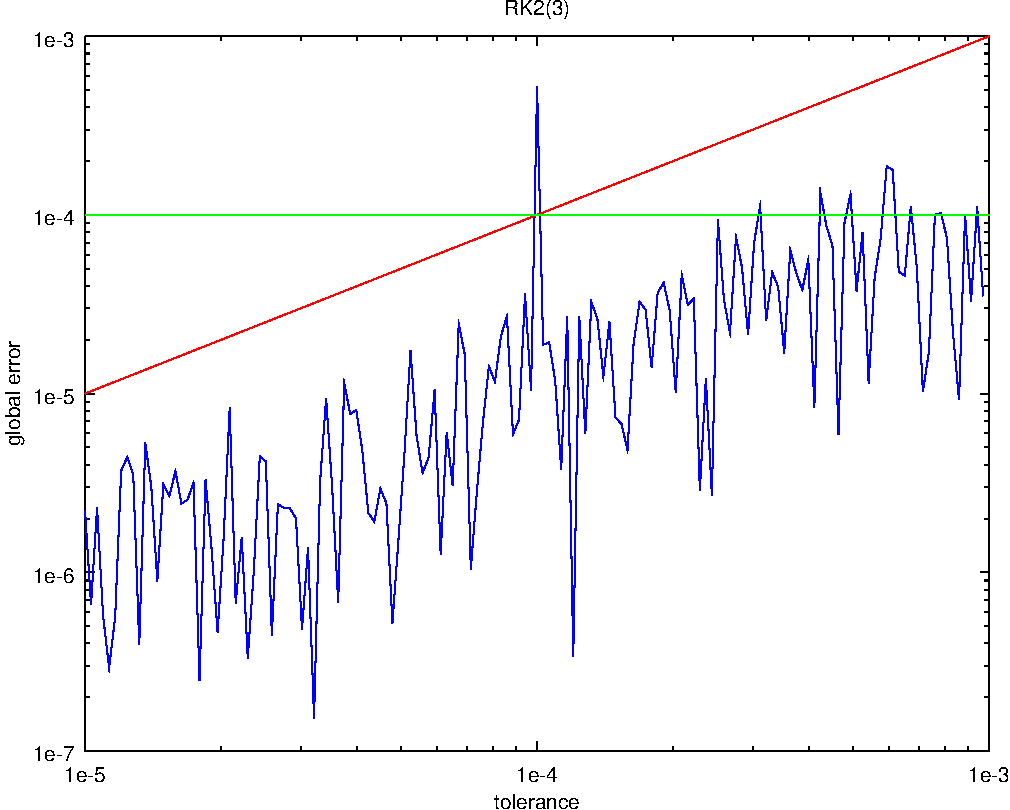
\includegraphics[scale=0.75]{figures/rk23globalError}
\end{figure}
 \ref{fig:rk23-global-error} akan menunjukkan garis lurus sempurna
yang sejajar dengan garis $y=x$, yang ditampilkan berwarna merah.
Gambar ini menunjukkan bahwa sebagian besar toleransi antara $10^{-5}$
dan $10^{-3}$ cukup untuk memberikan galat global sebesar $10^{-4}$
atau kurang, meskipun terdapat beberapa pengecualian, terutama satu
di sekitar $10^{-4}$. Gambar 
\begin{figure}
\caption{\label{fig:oscillatory}Solusi persamaan \ref{eq:oscillatory}}

\begin{centering}
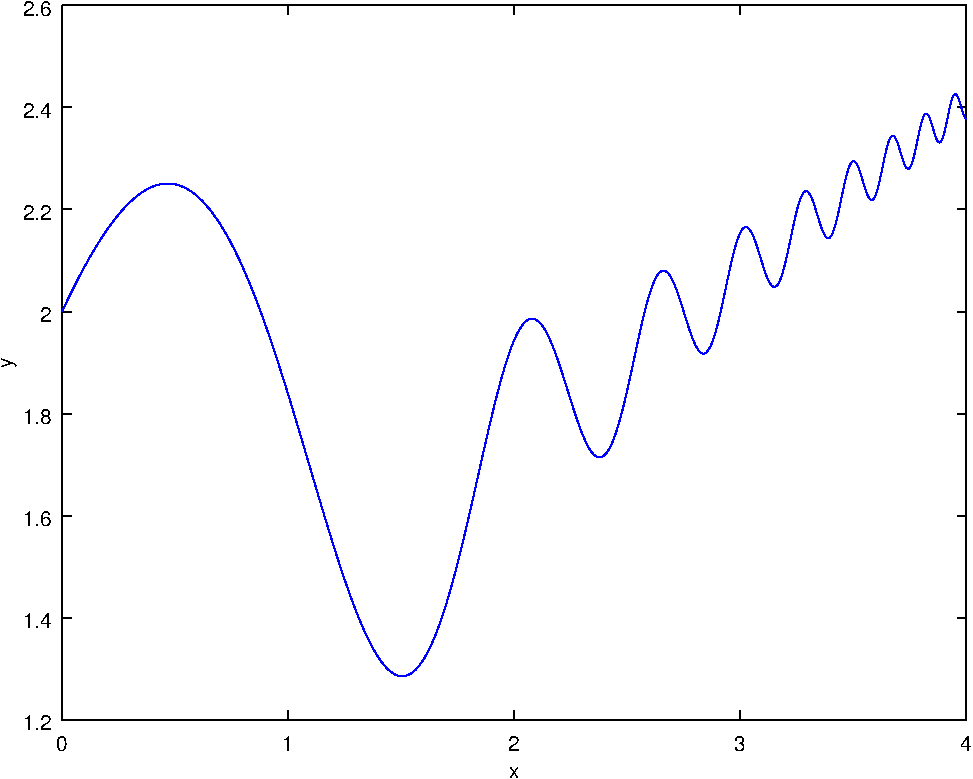
\includegraphics[scale=0.75]{figures/oscillatorySolution}
\par\end{centering}
\end{figure}
 \ref{fig:oscillatory} menunjukkan solusi pada selang $[0,4]$, yang
memperlihatkan osilasinya. Secara umum, membandingkan beberapa hampiran
yang menggunakan toleransi berbeda bukanlah cara mengendalikan galat
global. Galat global dapat dikendalikan dengan cukup baik dengan menskalakan
toleransi relatif terhadap ukuran langkah seiring berlangsungnya solusi
atau menggunakan galat relatif alih-alih galat absolut. Apa pun caranya,
persoalan ini menambahkan lapisan kompleksitas lain pada metode.
\item [{\ref{exc:ode-adaptive-28}:}] Ada dua kesulitan dalam masalah ini.
Kesulitan yang lebih sederhana ialah mengetahui besarnya galat hampiran
yang sebenarnya. PDB ini tidak dapat diselesaikan secara eksak, sehingga
kita tidak dapat menghitung solusi eksaknya. Kita tentu dapat menjalankan
metode dengan toleransi $10^{-4}$, tetapi ini hanyalah galat pemenggalan
\textit{lokal}. Galat ini tidak serta-merta menghasilkan taksiran
apa pun untuk galat \textit{global} (total galat yang terakumulasi
pada langkah terakhir). Sering kali, keduanya akan memiliki magnitudo
yang serupa, tetapi hal itu sama sekali tidak terjamin. Bagaimanapun,
berikut adalah hasil menjalankan metode dengan ukuran langkah awal
$\frac{1}{10}$ dan toleransi $10^{-4}$:

\begin{lyxcode}
>\textcompwordmark >~f=@(x,y)~(x\textasciicircum 2+y)/(x-y\textasciicircum 2)

f~=

@(x,~y)~(x~\textasciicircum ~2~+~y)~/~(x~-~y~\textasciicircum ~2)

>\textcompwordmark >~{[}y,x{]}=rk23(f,0,5,3,1/10,1e-4,100000);

>\textcompwordmark >~y(length(y))

ans~=~~3.66765768487404

>\textcompwordmark >~length(y)

ans~=~~17
\end{lyxcode}
yang menunjukkan bahwa $y(4)\approx3.66765$. Meskipun kita cukup
yakin bahwa ini merupakan taksiran yang wajar (misalnya dengan galat
tidak lebih dari $10^{-2}$), kita tentu tidak boleh mengklaim bahwa
galatnya kurang dari, atau bahkan benar-benar mendekati $10^{-4}$.
Algoritma tersebut memerlukan 17 langkah untuk mencapai hasil, sehingga
galat hanya sempat sedikit terakumulasi. Jika sangat penting untuk
mengetahui bahwa taksiran tersebut akurat sampai ke $10^{-4}$ atau
lebih baik, hasilnya dapat dibandingkan dengan hasil kedua yang menggunakan
toleransi lebih kecil:
\begin{lyxcode}
>\textcompwordmark >~{[}y,x{]}=rk23(f,0,5,3,1/10,1e-5,100000);

>\textcompwordmark >~y(length(y))

ans~=~~3.66757804370410
\end{lyxcode}
Selisih antara kedua taksiran kira-kira $7.96(10)^{-5}$. Hal ini
menunjukkan bahwa galat pada taksiran pertama kemungkinan tepat sekitar
$10^{-4}$. Namun, bukti ini pun sama sekali belum meyakinkan. Kesulitan
kedua adalah bahwa penyesuaian kecil pada toleransi dapat menyebabkan
perubahan besar pada galat global. Galat global sebagai fungsi toleransi
bersifat kasar dan tak kontinu (lihat Gambar \ref{fig:rk23-global-error-2}).
Jika galat global berskala sempurna dengan galat pemenggalan, Gambar
\begin{figure}
\caption{\label{fig:rk23-global-error-2}grafik log-log toleransi terhadap
galat global}

\centering{}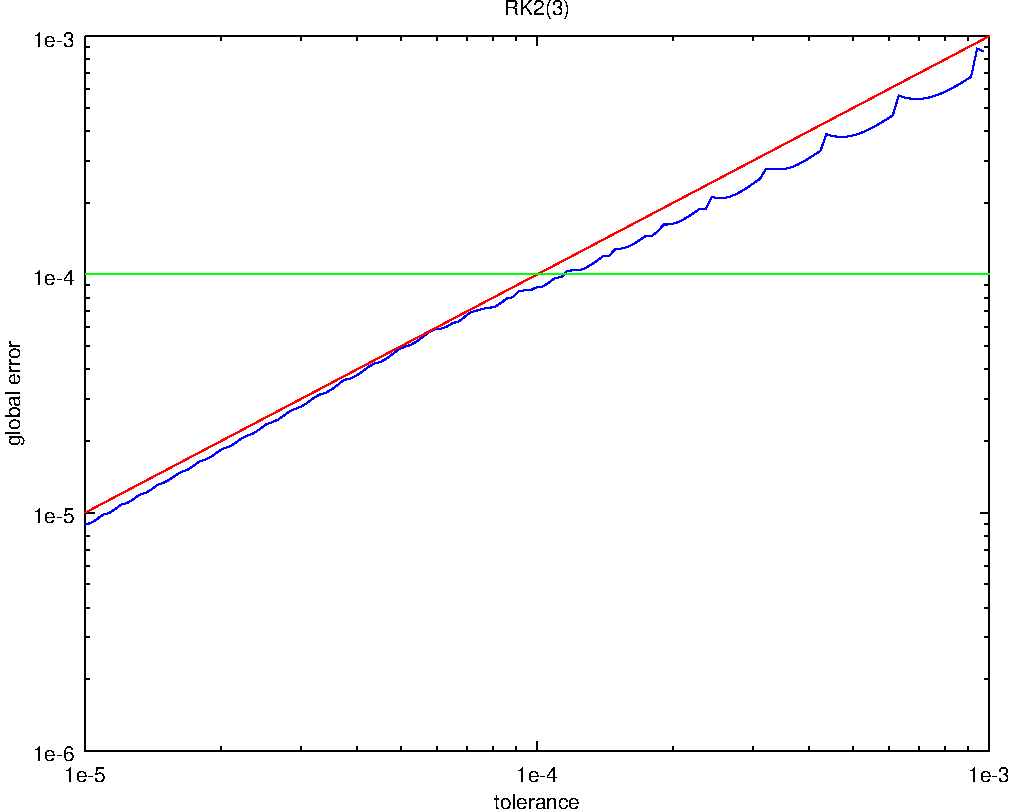
\includegraphics[scale=0.75]{figures/rk23globalError2}
\end{figure}
 \ref{fig:rk23-global-error-2} akan menunjukkan garis lurus sempurna
yang sejajar dengan garis $y=x$, yang ditampilkan berwarna merah.
Gambar ini menunjukkan bahwa sebagian besar toleransi antara $10^{-5}$
dan $10^{-3}$ cukup untuk memberikan galat global sebesar $10^{-4}$
atau kurang, meskipun mungkin ada beberapa pengecualian yang tidak
diplot. Gambar 
\begin{figure}
\caption{\label{fig:non-oscillatory}Solusi persamaan \ref{eq:non-oscillatory}}

\centering{}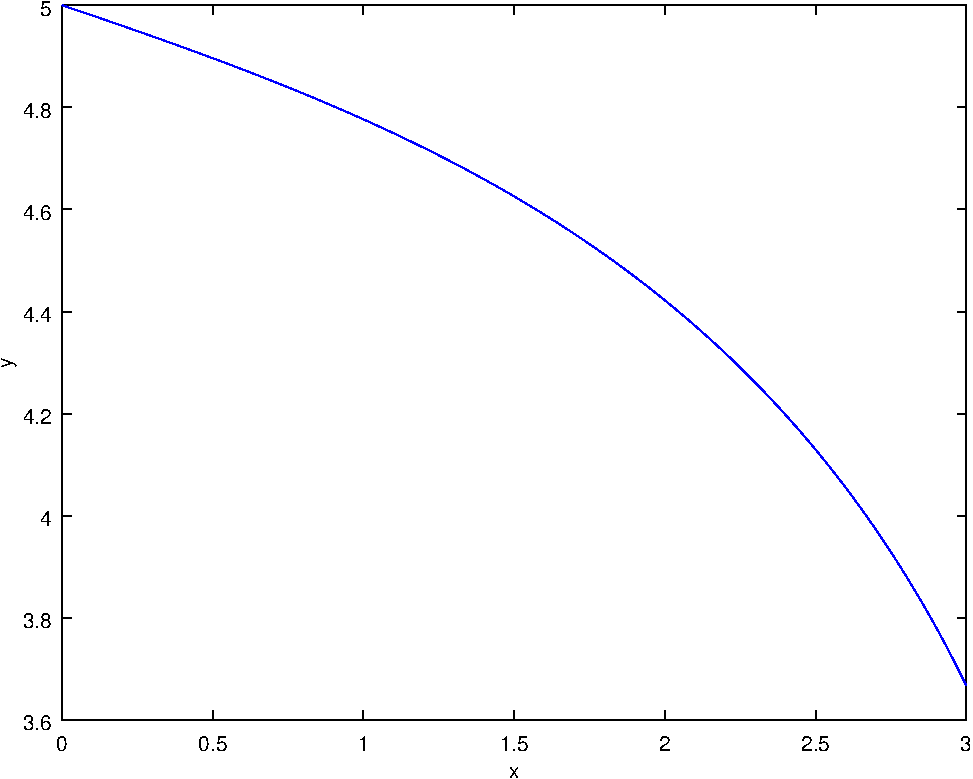
\includegraphics[scale=0.75]{figures/non-oscillatory}
\end{figure}
 \ref{fig:non-oscillatory} menunjukkan solusi pada selang $[0,3]$.
Secara umum, membandingkan beberapa hampiran yang menggunakan toleransi
berbeda bukanlah cara mengendalikan galat global. Galat global dapat
dikendalikan dengan cukup baik dengan menskalakan toleransi relatif
terhadap ukuran langkah seiring berlangsungnya solusi atau menggunakan
galat relatif alih-alih galat absolut. Apa pun caranya, persoalan
ini menambahkan lapisan kompleksitas lain pada metode.
\end{description}

